% To compile:
%   pdflatex blue.tex
%   makeindex blue.idx
%   pdflatex blue.tex
\documentclass[11pt]{memoir}
\usepackage[usenames,dvipsnames]{color}
\usepackage{bbding}  % for checkmark and X
\usepackage{dingbat}  % for leftthumbsup
\usepackage{array}           % For double-column exercises.
\usepackage{longtable}       % For double-column exercises.
\usepackage[normalem]{ulem}  % For strikethrough.
\usepackage{paralist}
\usepackage{enumitem}        % To "resume" enumerated lists.
\usepackage{epsfig}
\usepackage[nokeyprefix]{refstyle}
\usepackage{afterpage}
\usepackage{aurical}
\usepackage[T1]{fontenc}
\usepackage{varwidth}
\usepackage{multicol}
\usepackage{fancybox}
\usepackage[makeidx]{hvindex}
\usepackage{textcomp}
\usepackage{fancyvrb}
\usepackage{footnote}
\usepackage{makecell}
\usepackage{amsmath,amsthm,amsfonts,amssymb,latexsym}
\usepackage{MnSymbol}
\usepackage{wasysym}
\usepackage{float}
\usepackage{wrapfig}
\usepackage[hidelinks]{hyperref}
\usepackage[width=.9\textwidth,singlelinecheck=true,skip=1pt,font=small,labelfont=bf]{caption}
\usepackage{tabularx}


% Lulu.com
%\setstocksize{23.389cm}{15.593cm}
%\settrimmedsize{\stockheight}{\stockwidth}{*}
%\settrims{0pt}{0pt}

% Blurb.com
%\setstocksize{9.25in}{6.125in}
%\settrimmedsize{9in}{6in}{*}
%\settrims{.125in}{.125in}

% Amazon.com
\setstocksize{9in}{6in}
\settrimmedsize{9in}{6in}{*}
\settrims{0pt}{0pt}

\setlxvchars
\settypeblocksize{*}{\lxvchars}{1.618}

%\setlrmargins{*}{*}{.618}
\setlrmargins{*}{1.2cm}{.618}

% Lulu.com
%\setulmargins{110pt}{*}{*}

% Blurb.com
\setulmargins{80pt}{*}{*}
\setheaderspaces{50pt}{*}{1.618}

\checkandfixthelayout

\newcommand{\freakingtilde}{\raisebox{0.5ex}{\texttildelow}}

\makesavenoteenv{tabular}  % to allow footnotes in tables
\makesavenoteenv{figure}  % to allow footnotes in tables

\definecolor{darkgreen}{rgb}{0,.55,0}
\definecolor{darkred}{rgb}{.75,0,0}


%\captionsetup{width=.9\textwidth}

%\usepackage{enumerate}

% Crazy macro from:
% https://tex.stackexchange.com/questions/36401/drawing-boxes-around-words
% Used in "discovering" chapter.
\def\bluebox#1{\leavevmode \setbox0=\hbox{#1}%
   \dimen0=\wd0 \edef\posxA{\expandafter\ignorept\the\dimen0 \space}%
   \hbox{\kern3pt\pdfliteral{q .8 .8 1 rg .8 .8 1 RG .9963 0 0 .9963 0 0 cm 1
j 1 J 6 w
                             0 0 m 0 5 l \posxA 5 l \posxA 0 l 0 0 l B Q}%
         \box0 \kern3pt}%
}
{\lccode`\?=`\p \lccode`\!=`\t  \lowercase{\gdef\ignorept#1?!{#1}}}

\makeindex

\newenvironment{custommargins}[2]%
  {\addtolength{\leftskip}{#1}\addtolength{\rightskip}{#2}}{\par}

%% Set left margin - The default is 1 inch, so the following
%% command sets a 2-inch left margin.
%\setlength{\oddsidemargin}{1in}
%\setlength{\evensidemargin}{0in}
%% Set width of the text - What is left will be the right margin.
%% In this case, right margin is 8.5in - 1.25in - 6in = 1.25in.
%\setlength{\textwidth}{5.5in}
%
%% Set top margin - The default is 1 inch, so the following
%% command sets a 0.75-inch top margin.
%\setlength{\topmargin}{.75in}
%
%% Set height of the text - What is left will be the bottom margin.
%% In this case, bottom margin is 11in - 0.75in - 9.5in = 0.75in
%\setlength{\textheight}{7.25in}

\setlength{\parindent}{0pt}
\setlength{\baselineskip}{1.5pt}
\setlength{\parskip}{6pt}

\begin{document}

\title{{\Huge Blueprints:}\\
{\Large Creating, Describing, and Implementing Designs}\\
{\Large for Larger-scale Software Projects}\\{\small version 2.1.1}}
\author{Stephen Davies, Ph.D.\\Computer Science Department\\University of Mary Washington}
\date{}
\maketitle


\thispagestyle{empty}

Copyright \textcopyright \ 2021 Stephen Davies.

\bigskip

University of Mary Washington\\
Department of Computer Science\\
James Farmer Hall\\
1301 College Avenue\\
Fredericksburg, VA  22401

\vspace{.4in}

Permission is granted to copy, distribute, transmit and adapt this work under a
Creative Commons Attribution-ShareAlike 4.0 International License:

\begin{center}

\includegraphics{cc_license.png}\\
\smallskip
\url{http://creativecommons.org/licenses/by-sa/4.0/}
\end{center}

\vspace{.2in}
If you are interested in distributing a commercial version of this work, please
contact the author at \texttt{stephen@umw.edu}.

\vspace{.4in}
The \LaTeX source for this book is available from:
\url{https://github.com/rockladyeagles/blueprints}.

\vspace{1.8in}
Cover art copyright \textcopyright \ 2020 Stephen Davies.
Images courtesy of \url{photoeverywhere.co.uk} and \url{PNGio.com}.

\frontmatter

\renewcommand{\contentsname}{Contents}

% Add empty page to get to a multiple of 12 (312 total pages).
\begingroup
  \null
  \newpage
\endgroup

\setcounter{tocdepth}{0}
\tableofcontents

% 
\chapter{Preface}
Coming soon.


\setcounter{chapter}{0}

\mainmatter

\chapter{Getting off the ground}
\label{ch:gettingOff}

\index{command line}
\index{Linux}
\index{Unix}
Before we begin our study of object-oriented systems proper, we'll introduce
the command-line toolset we'll be using to construct our programs. We'll take
each of the most important tools out of our toolbox, lay them out before us on
a little mat, and learn what they're for.

\section{Why the command line?}

\index{CLI (command-line interface)}
\index{GUI (graphical user interface)}
Developing software in a command-line environment (sometimes abbreviated
``CLI'' for \textbf{command-line interface}, as opposed to a
``GUI\footnote{Commonly pronounced ``gooey.''}'' or \textbf{graphical user
interface}) involves typing white text in little black boxes. It requires
memorizing and regurgitating a variety of obscure commands. It demands exact
adherence to an inconsistent syntax, and exacts heavy penalties for mistakes,
all while providing only a very crude and clunky-looking interface.

It's natural to wonder why we would want to do this. After all, aren't
computer systems immeasurably more sophisticated now? If even end users run
fancy, graphical, forgiving apps, shouldn't computer scientists expect even
easier-to-use and sexier-looking stuff?

It may seem so, and in terms of the \textit{power} the tools provide, we'll
discover that indeed software developers are aptly equipped. But in some ways
it's a false expectation to assume that our toolset would be as \textit{easy}
to operate as that of an everyday user. After all, which is easier: to drive a
car, or to be a mechanic? Even though I enjoy cruise control and
auto-adjusting seats, I don't find it strange at all to learn that mechanics
still use socket wrenches to adjust piston assemblies.

Much of what makes a CLI so powerful is its expressiveness. A driver can press
any of the three or four cruise control functions the manufacturer provided.
But a mechanic can take any of hundreds of tools, tweak dozens of different
parts, and combine these adjustments in uncountable ways. That's the kind of 
flexibility the command line provides.

The difference between a CLI and a GUI is that with the latter, the user can
essentially do \textit{only what the tool designer anticipated she would want
to do.} There's no way she can express something that isn't one of the
tailor-made menu options.

When you use the command line, think of it as composing sentences, word by
word. A GUI comes with a repertoire of standard sentences you can choose from.
That makes it easy to do standard things, and hard to make silly mistakes. But
a CLI, being inherently language-based, is immeasurably more flexible. You can
write any (legal, grammatically correct) sentence you choose, even one the
designers of the CLI never thought of, and even one that you didn't know you'd
want to type until a moment ago. The bits and pieces can be combined in a
myriad of ways, just as nouns and verbs can.

\index{Finlayson, Ian}
There are other reasons as well that many developers live on the command line.
Among them are\footnote{Thanks to Ian Finlayson for capturing much of this
list.}:

\begin{itemize}
\itemsep.1em

\item \textbf{Speed.} It turns out to be way, way faster to type commands --
in combination with the various shortcuts and recall/edit operations -- than
it is to sift through menu options and such with a mouse. Trust me.

\index{remote access}
\index{shell}
\item \textbf{Remote access.} When you're running programs on your own device,
it's possible to do it with a GUI. But computer scientists very often have to
connect over the network to distant machines in order to tell them what to do.
Every time you need to configure a web server, for instance, or update a
publicly-accessible database, or run a time-consuming job on a parallel
cluster, or correct the data on your mobile device, you need a way to issue
commands to another machine through a very low-bandwidth channel. Opening a
command line ``shell'' to that remote device is by far the most common and
effective way to do this.

\index{scriptability}
\item \textbf{Scriptability.} There's just no good way to automate a sequence
of GUI operations. To explain to someone else how to accomplish something, you
have to painfully walk them through each operation (``go to the Start menu and
find Accessories, then in the Math menu choose Calculator...when it comes up,
right-click in the background and enable Advanced Options...'') which is
tedious and error-prone. It'd be nice if you could just send them a custom
command which would do all that. As a matter of fact, it would be nice if
\textit{you} could make a custom command which would do all that, so that you
could execute it many times without rehashing the same rigmarole. You'll find
that CLIs are eminently automatable in this way. You can create custom
commands called ``scripts'' that are combinations of other interacting
commands, and in this way you become master of your whole world.

\index{Cygwin}
\index{Mac OS X}
\index{Microsoft Windows}
\index{Raspberry Pi}
\index{Kindle}
\index{Terminal application}
\item \textbf{Consistency.} Graphical user interfaces are more different from
each other than CLIs are. Partly this is because nearly any CLI you're likely
to use is Unix/Linux-based\footnote{For our purposes, you can consider the
terms ``Unix'' and ``Linux'' exact synonyms. The Mac OS X command line
(available through the ``Terminal'' app) is Unix-based, too. Windows machines
aren't, but programs like ``Cygwin'' can be downloaded for free and provide a
Linux-like command-line veneer over the operating system.}, and hence they all
``speak the same language.'' It's great to be able to log on to different
laptops, web servers, your phone, your Kindle, or a Raspberry Pi and get the
same prompt that understands the same stuff.

\index{Linux}
\index{Unix}
\index{CLI (command-line interface)}
\item \textbf{Stability.} CLIs rarely change. When they do, it's very very
rarely in a non-backwards-compatible way. Every time a new graphical user
interface is released, you have to go through a period of hunting around and
finding out where everything is. With Unix/Linux, you can literally run
commands that were written last century and they will likely still work as is.

\end{itemize}

There's always a few students who despite the above benefits, resist learning
this material at first. I get it. It's like learning a new language, and the
immense effort to understand an alien world sure doesn't feel like it's going
to pay off any time soon. All I can say is that if you're not convinced it's
worth it, for now just think of it as something you have to master ``just
because your professor and the industry says so.'' My hope is that by the end
of this course, you're pleasantly surprised by seeing some payoff for your
hard work.


\section{The filesystem}
\index{filesystem}
\index{file}
\index{tree}
\index{directory}
\index{folder}

Okay. The backdrop for all our use of the Linux command-line interface is the
\textbf{filesystem}.\footnote{Often, not always, written as a single word as I
have it here.} Any general-purpose computer, no matter its architecture or OS,
has an area of permanent storage for user data. Interestingly, and
conveniently, they're all organized in pretty much the same way: as a
\textbf{tree} of \textbf{files} and \textbf{directories}. (Windows/Mac users
will be familiar with the term ``\textbf{folder},'' which \textit{means exactly
the same thing as ``directory.''}) In what follows, we'll be using a different
syntax (text instead of visual icons) to work with what is conceptually the
same organizational structure you're used to on your own computer.

\subsection{Files and directories}

\index{filesystem extension}
A file is simply any named chunk of stuff on your disk. Images, .mp3 tunes,
Word docs, and (importantly) plain text files are all in this category. On
Windows, you're used to each of these files having a filesystem ``extension''
designating its type: ``.doc'' means a Word doc, and ``.jpg'' means an image
file, for example. This is sort of true with Linux, although the rules are
a bit looser. Not all files have extensions at all, and when they do, it's
more a signal that they're intended to be treated a certain way than a
hard-and-fast requirement.

\index{java file@\texttt{.java} file}
The most important files you'll work with in this class will have a
\texttt{.java} extension. These are your Java source files. You'll also work
with other various supporting files to make all the tools work correctly.
It's important to realize that \textit{a file is fundamentally just some data,
which can theoretically be opened and dealt with by any program}. When we say
that HamletPaper.doc ``\textit{is}'' a Word doc, what we really mean is that
its data is formatted in a certain way that the Microsoft Word application
expects to see, so it can render it on the screen for editing. But it is
possible to open that same HamletPaper.doc file with other programs and
manipulate its contents. This may seem sketchy, but it is actually a force for
good.

In particular, you'll be tempted this semester to think of a \texttt{.java}
file as ``a \texttt{vim} file,'' in the same way that you may think of an
\texttt{.xls} file as ``an Excel file.'' I hope to eventually break you of this
habit, as you learn to see files as text or data that is actually independent
of what kind of program might be used to open and manipulate it.

\index{directory}
A directory is a container for files \textit{and also other directories}. That
last italicized phrase is what gives rise to the overall tree structure of the
filesystem, as discussed in the following section.

\index{Foreman, George}
By the way, every file and directory \textit{in a particular directory} must
have a unique name. You can't have a file called ``DireStraits.mp3'' and
another one also called ``DireStraits.mp3'' sitting there in the same folder:
it's a name collision. However, it's perfectly permissible to have two files
with the same name in different directories. This is kind of like how there
isn't more than one ``Stephen'' in my immediate family (that would be
confusing\footnote{With apologies to boxing legend George Foreman, who named
all four of his children ``George.'' That practice is not
filesystem-compatible.}), but there are of course many ``Stephens'' in the
world.

\subsection{The filesystem tree}

\index{tree}
\index{filesystem}
\index{directory!parent}
\index{parent directory}
The files and directories in a filesystem form a nested, hierarchical
structure called a \textbf{tree} (see Fig.~\ref{fig:tree}). I have drawn two
kinds of nodes in this tree: directories (yellow ovals) and files (blue
boxes). As expected, some of the directories have arrows coming out of them,
but none of the files do. The elements that a directory is pointing to are the
contents it contains: \textit{e.g.}, the left-most ``\texttt{america}''
directory contains another directory (``\texttt{nation}'') and also the file
\texttt{A.txt}. We use the term \textbf{parent directory} to mean the
directory immediately above an entry in the filesystem; the left-most
\texttt{A.txt} file's parent directory is the \texttt{america} directory we
just spoke of.

\begin{figure}[ht]
\centering
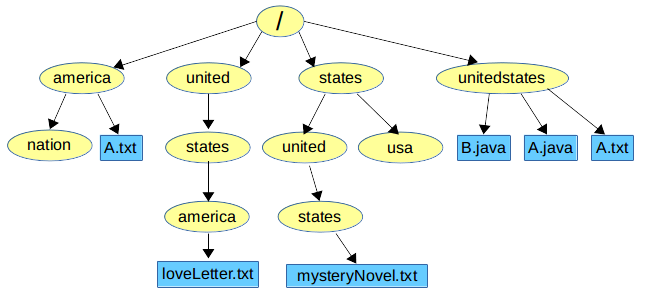
\includegraphics[width=0.9\textwidth]{tree.png}  %650x300
\caption{The Linux filesystem, in pictorial form.}
\label{fig:tree}
\end{figure}

Note that in order to keep you on your toes, I've given several entries in
this example filesystem the same name: in addition to a couple different
\texttt{america}s, we've got several \texttt{states}, multiple different
\texttt{A.txt}s, etc. In no case, however, are the duplicately-named entries
in the same directory. (Convince yourself of that fact.)

\subsubsection{Only one surprise}

\index{Microsoft Windows}
So far this is pretty easy. And it won't get much harder. But here's the one
thing you have to get used to: with a CLI, \textit{we won't ever actually see
that filesystem picture visually.} It's there, but we don't explicitly view it
in graphical form. Instead, there will be a textual way of referring to every
file and directory. It's straightforward, but can be a bit of a shock to those
coming from point-and-click systems like Windows.

\subsection{The ``current'' (or ``working'') directory}

\index{directory!current}
\index{directory!working}
\index{current directory}
\index{working directory}
One vital concept to grasp is that every time we issue a command or run a
program in Linux, we are doing so \textit{within the context of a particular
directory}. Conceptually, we think of being ``in'' a certain directory at any
point in time. We call this directory ``the \textbf{current directory}'' or
``the \textbf{working directory}'', and we'll learn commands to find out what
it is and to change it to something else.

Which one we're ``in'' has a crucial impact on what happens when we execute a
command. For instance, if our current directory is the far-left
\texttt{america} directory, and we issue a command that does something to
``\texttt{A.txt}'', it would act on the left-most \texttt{A.txt} file, since
it's the one within the current directory. But if our current directory were
\texttt{unitedstates}, ``\texttt{A.txt}'' would instead mean the far-right blue
node.

I've found that failure to understand the current directory is one of the most
common trouble spots for beginning Linux programmers.

\subsubsection{The root directory}

\index{directory!root}
\index{root directory}
\index{tree}
Okay, back to the filesystem as a whole. At the top of the tree is the
\textbf{root directory}, which has no parents. (This is often disorienting to
non-computer-scientists, since in the real world trees actually grow
\textit{up}, not down. But in computer science, we always draw trees growing
down from the root.)

\index{backslash}
\index{forward slash}
\index{slash}
\index{Microsoft Windows}
The root directory is the anchor point of the entire filesystem: it ultimately
contains everything under it. It also has a very strange name: ``\texttt{/}'',
pronounced ``slash.'' (This is a ``forward slash,'' by the way, to the left of
your right-most Shift key, not a ``backslash.'' Oddly, most Windows systems
use a backslash ``\texttt{\textbackslash}'' for this instead.) Stay awake,
because this ``\texttt{/}'' character will shortly mean something very
different as well.

\subsubsection{Paths}

\index{path}
\index{directory}
\index{file}
It should be apparent to you that as a consequence of this nested tree
structure, you can ``reach'' every element from the root directory by
traversing from arrow to arrow. Furthermore, you can do so in only one way.
For instance, the \texttt{B.java} file can be reached from the root by going
from ``\texttt{/}'' to \texttt{unitedstates} to \texttt{B.java}. And that's the
\textit{only} way to get there. You can reach \texttt{loveLetter.txt} by going
from ``\texttt{/}'' through \texttt{united}, \texttt{states}, and
\texttt{america}, in that order. This is true for every file and directory.

What this means is that every entry has a unique \textbf{path}, and we can
express it in text as well as in a diagram. Take the \texttt{B.java} file for
example. Its path is:

\quad\quad \texttt{/unitedstates/B.java}

\index{slash}
Look very carefully at that string as we dissect it. The most important thing
to grasp is that the two slash (``\texttt{/}'') characters \textit{each mean
something different}. The first one means ``the root directory, which is
called slash.'' But the second one is merely a separator, delimiting the
\texttt{unitedstates} from the \texttt{B.java}. So this path means
``\textit{start at the root directory}, go down to its \texttt{unitedstates}
entry (which is a directory), and there you have the \texttt{B.java} file.''

Similarly, the path to \texttt{loveLetter.txt} is:

\quad\quad \texttt{/united/states/america/loveLetter.txt}

\index{slash}
(Note that the slash between \texttt{united} and \texttt{states} makes all the
difference in the world: if it weren't there, we'd be starting our descent
through the right-most \texttt{unitedstates} directory as before.)

\index{path!absolute}
\index{absolute path}
\index{planet}
\index{path!relative}
\index{relative path}
These paths are called \textbf{absolute paths} because they \textit{start with
a slash}. This means that they give the complete, start-from-the-top position
of a particular file or directory. It's kind of like referring to a building
by its complete address, including city, state, zip code, country, and planet.
Often we want a short-hand way of referring to an entry without specifying its
entire absolute path. To do so, we use a \textbf{relative path}.

\index{directory!current}
\index{current directory}
A relative path is relative \textit{to the current directory}. And it does
\textit{\textbf{not}} begin with a slash. Instead, it gives directory names,
separated by slashes, indicating where to start descending \textit{from the
current directory}.

For example, let's say the current directory was ``\texttt{/states}''. And
suppose I used this relative path:

\quad\quad \texttt{united/states/mysteryNovel.txt}

(Note \textit{carefully} that it has \textit{no} initial slash!) This relative
path would instruct us to \textit{start at the current directory}
(\texttt{/states}) and from there traverse down to \texttt{united},
\texttt{states}, and then finally \texttt{mysteryNovel.txt}. Obviously, where
you end up is critically dependent on where you start -- on what the current
directory is.

\index{directory!current}
\index{current directory}
To test your understanding, realize that in this case where the current
directory is \texttt{/states}, there is no such file called
\texttt{united/states/america/loveLetter.txt}. In fact, even 
\texttt{united/states/america} doesn't exist. However, if we changed the
current directory to be the root (``\texttt{/}''), suddenly the relative path
\texttt{united/states/ america/loveLetter.txt} would be legit.

\section{Linux A-B-C's}

\index{Unix}
\index{Linux}
\index{filesystem}
\index{file}
\index{directory}
With the filesystem always hovering in the background, let's introduce the
first basic Linux commands to work with the files and directories. These
commands are so basic that they're like the alphabet of speaking any Linux
sentence. Using them should eventually be as familiar and effortless as
clicking the mouse.

\index{prompt}
\index{dollar sign (\texttt{\$})}
In all that follows, I will precede anything you are to type on the Linux
command line with a dollar sign \textbf{prompt}:

\begin{Verbatim}[fontsize=\small]
$
\end{Verbatim}

To execute a command, you do \textit{not} type the prompt itself: it's just
there to indicate ``now is an appropriate time and place to enter a Linux
command.'' Just type the stuff after it.

\index{directory!current}
\index{current directory}
Also, depending on your system and configuration, your prompt may look
different or have other information in it. One common setting, for instance,
is for the current directory to always appear as the prompt. (I personally
hate that, since it makes some commands start at different horizontal
locations as I work, plus it consumes a lot of space.) No matter what, though,
just mentally substitute ``the dollar sign'' for ``whatever your Linux prompt
is.''

\newcommand{\bigline}{\begin{center} \line(1,0){300} \end{center}}


\begin{enumerate}
\itemsep.1em
\item \textbf{\texttt{pwd}}

\index{pwd@\texttt{pwd}}
Your first command stands for ``\textbf{p}rint \textbf{w}orking
\textbf{d}irectory,'' and simply tells you what the current directory is at any
point in time. For example:

\begin{Verbatim}[fontsize=\small]
$ pwd
/united/states
\end{Verbatim}

tells you that you're currently ``in'' the \texttt{states} directory, which is
contained within the \texttt{united} directory, which is contained within the
root directory.

\textbf{Tip:} get in the habit of typing \texttt{pwd} a \textit{lot},
especially at first. Get ingrained in your brain the concept of ``where am I
in the filesystem right now?'' because it matters, yet is not in your face
except when you type this command.

\bigline
\item \textbf{\texttt{cd}}

\index{cd@\texttt{cd}}
\texttt{cd} stands for ``\textbf{c}hange \textbf{d}irectory'' and is how you
move to another place. You give it an \textbf{argument} (kind of like passing
a parameter to a function call in a programming language, although we don't
use parentheses or commas here) which is where you want to go:

\begin{Verbatim}[fontsize=\small]
$ cd  /america/nation
\end{Verbatim}

Here, I've specified an absolute path. If I now execute \texttt{pwd}, I see
that it worked:
\begin{Verbatim}[fontsize=\small]
$ pwd
/america/nation
\end{Verbatim}

\index{relative path}
\index{path!relative}
\index{absolute path}
\index{path!absolute}
More common is to specify a relative path. If we go back to our original
location:

\begin{Verbatim}[fontsize=\small]
$ cd  /united/states
$ pwd
/united/states
\end{Verbatim}

we can then say ``go \textit{from here} into the \texttt{america} directory'':

\begin{Verbatim}[fontsize=\small]
$ cd  america
$ pwd
/united/states/america
\end{Verbatim}

\index{cd@\texttt{cd}}
\index{pwd@\texttt{pwd}}
I can't overestimate how important it is to notice that in the previous
\texttt{cd} command, I did \textit{not} include a slash before
\texttt{america}. If I had, it would have been an absolute path, and I would
have gone to a completely different part of the filesystem:

\begin{Verbatim}[fontsize=\small]
$ cd  /america
$ pwd
/america
\end{Verbatim}

\subsubsection{``Special'' directory shortcuts}

\index{directory!shortcuts}
\index{special directory shortcuts}
This is a good time to mention that when you are specifying paths, there are
three very common shortcuts that you'll want to know about.


\begin{itemize}
\itemsep1em

\index{directory!current}
\index{current directory}
\item The current directory: \texttt{\textbf{.}}

A plain-ol' dot (period) is used to mean ``the current directory.'' There's no
obvious uses for this yet, but believe me, it comes up \textit{all} the time,
so just memorize it. A useless example for now:

\begin{Verbatim}[fontsize=\small]
$ pwd
/united/states
$ cd  ./america
$ pwd
/united/states/america
\end{Verbatim}

So ``\texttt{./america}'' is another way of saying ``\texttt{america}''. (Told
you this example was useless.)

\item The parent directory: \texttt{\textbf{..}}

\index{directory!parent}
\index{parent directory}
More immediately useful is the double-dot, which means ``the parent of the
current directory.'' If we're in \texttt{/united/states} and want to go to
\texttt{/united}, one way to do it is:

\begin{Verbatim}[fontsize=\small]
$ cd  ..
$ pwd
/united
\end{Verbatim}

We can also join this with additional relative path stuff to move around the
hierarchy in various ways:

\begin{Verbatim}[fontsize=\small]
$ pwd
/states/united
$ cd  ../usa
$ pwd
/states/usa
\end{Verbatim}

\index{directory!sibling}
\index{sibling directory}
\index{directory!child}
\index{child directory}
Here we went to a ``sibling'' directory by ``going up one, and then down to a
different child.''

\item The home directory: \texttt{\textbf{\freakingtilde}}

\index{directory!home}
\index{home directory}
A shortcut for ``the home directory'' (which means ``the current directory when
you first log in'') is a tilde. It's commonly used in conjunction with other
relative path stuff, like the last double-dot example, above.

Your home directory (which you can verify by just typing \texttt{pwd} when
you first log in) will probably be something like \texttt{/home/joeschmo}.
Suppose it is. Then, if you type:

\begin{Verbatim}[fontsize=\small]
$ pwd
/somewhere/else/in/the/filesystem
$ cd  ~/shortStories/scifi
$ pwd
/home/joeschmo/shortStories/scifi
\end{Verbatim}

you can go to any of your subdirectories.

\end{itemize}

\bigline
\item \textbf{\texttt{ls}}

\index{ls@\texttt{ls}}
While \texttt{pwd} tells you what the current directory is, \texttt{ls}
command (``\textbf{l}i\textbf{s}t'') gives you its contents. If I type it while
in the \texttt{/america} directory, for instance, it tells me:

\begin{Verbatim}[fontsize=\small]
$ ls
nation   A.txt
\end{Verbatim}

there are the two entries from Figure~\ref{fig:tree}.

\index{ls@\texttt{ls}}
A few gotchas to be aware of here. First, there's no way from that listing to
tell that \texttt{nation} is a directory whereas \texttt{A.txt} is a file. If
you want to see that, you need to add the ``\texttt{-l}'' (a minus sign
followed by the lower-case letter ``ell'') option:

\begin{Verbatim}[fontsize=\small]
$ ls  -l
-rw-r--r-- 1 kyloren   sithlords   17 Sep  5 16:21 A.txt
drwxr-xr-x 2 kyloren   sithlords 4096 Sep  5 16:21 nation
\end{Verbatim}

Lots of clutter here. The key points:

\begin{compactitem}[-]
\item The far-left character on each line is either a ``\texttt{-}'' or a
``\texttt{d}'', indicating file or directory.
\index{file!owner}
\item Files in Linux have ``owners,'' meaning specific users who created them
and have permissions to manage them. Both of these entries are evidently owned
by user \texttt{kyloren}.
\item The \texttt{17} and \texttt{4096} are file sizes (in bytes).
\item You can see the date and time each entry was last modified.
\end{compactitem}

\index{long file listing}
\index{option}
The ``\texttt{-l}'' stands for ``\textbf{l}ong file listing.'' Most Linux
commands have a bevy of different options you can specify when you execute
them, most often beginning with a minus sign.

Another important one for the \texttt{ls} command is ``\texttt{-a}'' which
stands for ``\textbf{a}ll files, please.'' If that sounds like a strange
option, that's because it is. It turns out that \texttt{ls} by default doesn't
show you all the files; in particular, \textit{it omits those whose names
start with a dot (.).} Why? There are reasons. The only time this will be
relevant to you soon is when you want to work with the \texttt{.bashrc} file,
as described later in this chapter. You'd have to type ``\texttt{ls -a}'' in
your home directory to actually see it in the listing.


\bigline
\vspace{.1in}
\index{cd@\texttt{cd}}
\index{pwd@\texttt{pwd}}
\index{ls@\texttt{ls}}
*The above three commands -- \texttt{pwd}, \texttt{cd}, and \texttt{ls}, go
together like Rey, Finn, and Poe. Get in the habit of using them literally
every minute you're working on the Linux command line.
\vspace{.1in}
\bigline

\item \textbf{\texttt{mkdir}}

\index{mkdir@\texttt{mkdir}}
To create a directory in the first place, use the \texttt{mkdir} command and
give it the name:

\begin{Verbatim}[fontsize=\small]
$ mkdir  evilplans
\end{Verbatim}

This new \texttt{evilplans} directory will be created inside the current
directory.

Note carefully that \textit{making a directory does not automatically put you
in it!} Lots of beginners mistakenly think this will happen, but you can see
that it does not:

\begin{Verbatim}[fontsize=\small]
$ pwd
/home/kyloren
$ mkdir  evilplans
$ pwd
/home/kyloren
\end{Verbatim}

\index{cd@\texttt{cd}}
You have to \texttt{cd} as a separate step if you want to now be in
\texttt{evilplans}:

\begin{Verbatim}[fontsize=\small]
$ cd  evilplans
$ pwd
/home/kyloren/evilplans
\end{Verbatim}

\index{directory!parent}
A useful option to \texttt{mkdir} is the ``\texttt{-p}'' option which means
``make all \textbf{p}arent directories as necessary.'' This lets us create a
deeply-nested structure all in one fell swoop:

\begin{Verbatim}[fontsize=\small]
$ mkdir  -p  find/luke/skywalker/now
$ cd  find/luke/skywalker/now
$ pwd
/home/kyloren/find/luke/skywalker/now
\end{Verbatim}

\bigline

\item \textbf{\texttt{cp}}
\index{cp@\texttt{cp}}
\index{file!copying}

To make a copy of a file, use \texttt{cp} and give it \textit{two} arguments,
a source and a destination. If I type:

\begin{Verbatim}[fontsize=\small]
$ cp  A.txt  Q.txt
\end{Verbatim}

I will now have two exact copies of the file which can be independently
modified:

\begin{Verbatim}[fontsize=\small]
$ ls
nation   A.txt   Q.txt
\end{Verbatim}

I can also use this to make a (same-named) copy of a file to a different
location, by providing a directory as the second argument:

\begin{Verbatim}[fontsize=\small]
$ cp  A.txt  /states/usa
$ cd  /states/usa
$ ls
A.txt
\end{Verbatim}

\bigline

\item \textbf{\texttt{mv}}
\index{mv@\texttt{mv}}
\index{file!renaming}

\texttt{mv} has pretty much the same effect as \texttt{cp}, except that it
does not retain the original copy. This command can be used to rename a file
(``\texttt{\$ mv oldfilename newfilename}'') as well as to change a file's
location.

\bigline

\item \textbf{\texttt{vim}} (and \texttt{vimtutor})
\index{vim@\texttt{vim}}

It's really ludicrous to include this command in amongst all the others, when
its ins-and-outs could (and do) occupy entire textbooks in their own right.
\texttt{vim} is a text editor program with a zillion amazing features which
you will use this semester to write your programs. The normal way of creating
a file, in fact, will be this:

\begin{Verbatim}[fontsize=\small]
$ vim  notesOnTheResistance.txt
\end{Verbatim}

or this:

\begin{Verbatim}[fontsize=\small]
$ vim  DestroyGalacticRepublic.java
\end{Verbatim}

after which you will do loooooooooooots of other stuff way beyond the scope of
this book. That stuff will be cryptic and agonizing at first, but will
eventually become second-nature and give you the tremendous text editing power
you need to be a truly efficient software developer. It's kind of like
learning to use the Force for the first time.

\index{vimtutor@\texttt{vimtutor}}
For now, I'll make this (strong) suggestion: when you're first learning vim,
type this command (all one word) at the command line,

\begin{Verbatim}[fontsize=\small]
$ vimtutor
\end{Verbatim}

\index{Coke}
grab a Coke, and spend 30-40 minutes patiently reading and following the
instructions. This tutorial is quite good, and will teach you the very basics
of getting a file created and edited with this incredible tool.

\bigline

\item \textbf{\texttt{git}}
\label{introduceGit}
\index{git@\texttt{git}}
\index{version control system}

\texttt{git} is another one that doesn't really fit in this list, since it's
much more than just ``a command.'' For now, though, all you need to understand
is that it's a \textbf{version control system} that allows you to track and
manage the changes you make to your software over time. Up until now, you've
been dealing with the paradigm of ``the IDE always has the most recent copy of
my code, and that's the only version of it that exists.'' It turns out that
you'll need much more flexibility than that when you work on large systems.

Here's all you need to know at present:

\begin{compactitem}
\index{git@\texttt{git}!\texttt{git init}}
\index{repository@``repo'' (repository)}
\item The command ``\texttt{\$ git init .}'' (don't forget the dot at the end,
after a space) creates a git \textbf{repository}
(or ``\textbf{repo}'') in the current directory. That just means that your
current directory, and everything under it, are now ``under git's
management.'')
\index{git@\texttt{git}!\texttt{git add}}
\item You use ``\texttt{git add}'' to make git aware of
one or more files that you want it to track from that point forward. You'll
type ``\texttt{\$ git add }file1 file2 file3'' or however many files you want
to add at that point. Ordinarily you'll want to \texttt{git add} all of your
\texttt{.java} files.
\index{git@\texttt{git}!\texttt{git commit}}
\index{commit}
\index{snapshot}
\item When you've made a
significant change to one or more of your files that you want git to be aware
of, you'll enter this command:
\begin{Verbatim}[fontsize=\small]
$ git  commit  -a  -m  "A message describing the change."
\end{Verbatim}
Each such change is called a \textbf{commit}. Think of it as taking a
snapshot of your code that you can return to later.
\index{git@\texttt{git}!\texttt{git status}}
\index{git@\texttt{git}!\texttt{git log}}
\item ``\texttt{\$ git status}'' and ``\texttt{\$ git log}'' are two useful
commands that show the current state of your files as git sees them, and a
history of all the different commits you've made. Type them occasionally just
to get a feel for what kind of information they show.
\end{compactitem}

We'll talk much more about \texttt{git} later. For now, just know that it
exists, and type the commands verbatim when prompted.

\bigline
\item \textbf{\texttt{javac}} and \textbf{\texttt{java}}

\index{javac@\texttt{javac}}
\index{java@\texttt{java}}
\index{compiler}
\index{virtual machine}
\index{JVM (Java Virtual Machine)}
\index{JDK (Java Development Kit)}
\index{J2SE (``Java 2 Standard Edition'')}
\index{JRE (Java Runtime Environment)}

Now, finally to some programming stuff. On your Linux system, the Java
\textbf{compiler} (\textit{i.e.}, the program that converts your source code
into the form the computer needs to run it) is called \texttt{javac}, and the
\textbf{virtual machine} (the interpreter that runs your compiled code) is
called \texttt{java}. Both of these are part of the \textbf{JDK}, or ``Java
Development Kit,'' that you install in order to program in Java.\footnote{Just
to confuse you, the JDK has sometimes been called the ``Java SDK'' (``Java
Software Development Kit'') and the ``J2SE'' (``Java 2 Standard Edition'') in
the past, and you'll likely run across those acronyms as well. To confuse you
even more, the software you need to simply \textit{run} a Java program (as
opposed to writing your own) is called the ``JRE'' -- Java Runtime
Environment. Finally, to confuse you yet further, Java version numbers were
originally all ``one-dot-something'' (like ``Java 1.3'') but in 2004 they
ditched the ``one-dot'' and started naming the versions after the second
number alone. (So, the successor to ``Java 1.4'' was ``Java 5.'') This book
assumes you're on Java 8.}


\index{compiler}
To compile, you give \texttt{javac} all the Java files that are part of your
program:

\begin{Verbatim}[fontsize=\small]
$ javac  DestroyGalacticRepublic.java  Bombs.java  SinisterPlans.java
\end{Verbatim}

\index{java file@\texttt{.java} file}
\index{class file@\texttt{.class} file}
\index{main method@\texttt{main()} method}
which will produce either a \texttt{.class} file for each \texttt{.java} file,
or compiler errors for you to read. Finally, to run it, you give \texttt{java}
the name of \textit{the class that contains your \texttt{main()} method}:

\begin{Verbatim}[fontsize=\small]
$ java  DestroyGalacticRepublic
\end{Verbatim}

(Notice we don't include ``\texttt{.java}'' or ``\texttt{.class}'' here, and
notice we don't mention every Java class, only the one that has the
\texttt{main()}.)

\end{enumerate}

\section{The quickest path through the woods}

Whew. That was a lot. It's kind of like moving to another country: every
little thing, all at once, seems different.

All I can do is promise you it will get easier as you get used to that new
country. And there will be parts of it you will like -- maybe you'll even like
it better than the point-and-click country you grew up in.

\index{Hello World@``Hello, World"!'' program}
In the meantime, let's pull together all the steps to get a ``Hello World''
Java program running on the Linux command line.

\begin{enumerate}
\itemsep.1em
\item Log on to your Linux system, however you do that.
\item Create a directory to hold your project:
\begin{Verbatim}[fontsize=\small]
$ mkdir  myFirstProgram
\end{Verbatim}

\item And make sure to actually go there:
\begin{Verbatim}[fontsize=\small]
$ cd  myFirstProgram
\end{Verbatim}

\item Create a git repo to manage this project:
\begin{Verbatim}[fontsize=\small]
$ git  init  .
\end{Verbatim}

(and of course don't forget that pesky dot at the end.)

\item Now create a Java file:
\begin{Verbatim}[fontsize=\small]
$ vim  HelloWorld.java
\end{Verbatim}

\textbf{(You are now in \texttt{vim}. Everything you learned during your
\texttt{vimtutor} session, and everything you can get from a zillion different
``vim cheat sheets'' on the Internet, is relevant now. Good luck.)}

\item Give it these contents:
\begin{Verbatim}[fontsize=\small,frame=single]
class HelloWorld {
    public static void main(String args[]) {
        System.out.println("Yo 'sup dawg!");
    }
}
\end{Verbatim}

\item Save your file and exit \texttt{vim}.

\item Now compile it:
\begin{Verbatim}[fontsize=\small]
$ javac  HelloWorld.java
\end{Verbatim}

\item And, since it gave you no errors, run it:
\begin{Verbatim}[fontsize=\small]
$ java  HelloWorld
\end{Verbatim}

\end{enumerate}

It's a big bright world ahead of us. Go take a break and I'll see you next
chapter.


\chapter{The ``software crisis'' and encapsulation}

This book is going to dive deeply into a huge pile of nuts and bolts. But
before we take the leap into particulars, it's important to stand briefly at
the precipice and understand why we're jumping. What does ``object-oriented''
mean? What problem was it intended to solve? When was it invented and why?

\section{Ancient history}

A long time ago, in our own galaxy, a situation emerged which has been labeled
\textbf{the software crisis}. This crisis didn't happen at an instant in time;
it was a set of disagreeable circumstances which gradually evolved until it
became unbearable. The crisis is usually dated somewhere in the 1970's. This
was just as the high-tech computing industry was really starting to heat up,
on its way to permanently changing the lives of almost everyone on the planet.

Now ``crisis'' is an alarming word, designed to get your attention. It's worth
asking what all the hubbub was about. The immediate symptom may not strike you
as a three-alarm fire: it was simply that software projects were tending to
overrun their schedules.

The '70's were not a very plug-and-play era, since standards had not yet
evolved to facilitate intercompatibilities between devices or programs. So the
focus was often on building complete systems from the ground up. Engineering
teams would plan releases of key product lines that involved numerous
components, such as system architecture, hardware design and integration, data
collection and organization, system and network configuration, and software
development at both the operating system and the end user levels.

What managers discovered was that consistently, the \textit{software}
components of projects were coming in late and over-budget. Sometimes, they
didn't get finished at all. When they did, they were buggy and brittle. And
they were especially vulnerable to requirements changes: if circumstances were
discovered during the project that required a change in the way the software
needed to work, the software team was often strikingly unable to adapt to
this. They could be set back weeks or months to implement even a modest
change.

This astonished everyone at the time. After all, ``\textit{soft}ware'' -- a
pun on ``hardware'' -- was a term intended to convey the flexible, malleable
nature of computer programs as contrasted with physical devices. Software was
supposed to be easy to write and easy to change. That was the point. You
didn't need complex manufacturing processes: you needed a desktop computer and
a text editor. And you (seemingly) didn't face challenges of scale the way you
did with hardware: you could run out of room to put logic circuits on a chip
or a motherboard, but there was no limit to the size of a text file. 

So building complex stuff quickly, and turning on a dime when necessary, ought
to be easy to do in software. Right?

\subsection{Quantifying the crisis}

\begin{figure}[ht]
\centering
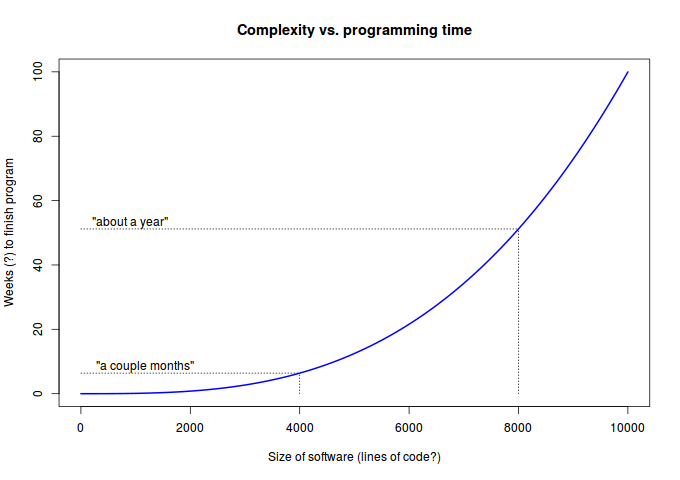
\includegraphics[width=0.7\textwidth]{complexityCurve.png}
\caption{The software crisis quantified: how long it took to complete a
program of various sizes. (Conceptual.)}
\label{fig:complexityCurve}
\end{figure}

\section{Software and complexity}

% The software crisis

% "soft"ware
% time vs. complexity curve

% Programming language diagram

\section{Dependencies}

\section{Encapsulation}

\section{Features of OO}

\section{Exercises}

Use an index card or a piece of paper folded lengthwise, and cover up the
right-hand column of the exercises below. Read each exercise in the
left-hand column, answer it in your mind, then slide the index card down to
reveal the answer and see if you're right! For every exercise you missed,
figure out why you missed it before moving on.

\begin{small}
\begin{enumerate}
\newcolumntype{Q}{>{\arraybackslash}m{.3\textwidth}}
\newcolumntype{A}{>{\arraybackslash}m{.6\textwidth}}
%\begin{longtable}{m{0.3\textwidth} || m{0.6\textwidth}}
\begin{longtable}{Q || A}
\hline
\item 
What key software problem was the OO paradigm invented to address?
&
Too many dependencies.
\\
\hline

\end{longtable}
\end{enumerate}
\end{small}


\chapter{Classes and objects}
\label{ch:classesObjects}

\index{object-oriented}
\index{class-oriented@``class-oriented''}
Java is called an ``object-oriented'' programming language. Now if \textit{I}
were King of the World, I would have called it a ``\textit{class}-oriented''
language instead. That's because in Java, you don't write code for objects,
but for \textit{classes}, and the code then defines the behavior of the
objects that are based on them.\footnote{There are other languages, for
instance JavaScript (no relation to Java), which do IMO deserve the term
``\textit{object}-oriented,'' since you can create code for individual objects
rather than classes, and not every object has to have a class at all.} You'll
sometimes hear people mistakenly say stuff like, ``I wrote some code for the
DatabaseConnection object today.'' It makes me wince. They weren't writing
``code for the object,'' but the code for a class.

\section{Terms}

\index{object}
\index{class@\texttt{class}}
\index{Venkman, Peter}
So here's a crucial pair of definitions. A \textbf{class} is a
\textit{category} of things. An \textbf{object} is a concrete \textit{example}
of a class. If ``University'' is a class, then ``UMW'' is an object; if
``Course'' is a class, then ``CPSC 240'' is an object. The difference is real,
and it is vitally important to keep at the forefront of your mind as you begin
your OO quest. Getting them mixed up is like Peter Venkman crossing the
streams.

\index{template}
\index{modeling}
You'll sometimes hear alternate definitions of these terms, like ``a class is
a template, and objects are copies of that template.'' This is better than
out-and-out confusion, but it still misses something important. It's an
operational definition, instead of a conceptual definition. It thinks of a
class and an object in terms of the mechanical way the virtual machine carries
out their duties, rather than in terms of \textit{modeling}, which is what
OOA\&D is all about.

\index{category}
In our world, every single software object will be a member of a category,
and that category will define everything about its inner structure and rules
of behavior.

\index{type}
\index{instance}
By the way, an important near-synonym for class is \textbf{type}. (It's only a
\textit{near}-synonym because primitive, non-classes like \texttt{int}s and
\texttt{boolean}s are also types.) An important exact synonym for object is
\textbf{instance}.

\index{instantiate}
\index{new@\texttt{new}}
In addition to those nouns, a big verb in our vocabulary will be the term
\textbf{instantiate}. It means ``to actually create an object of a particular
class.'' Some people use words like \textbf{construct} or \textbf{create} for
this, or even ``\texttt{new}'' (or ``\texttt{new} up'') as a verb, but for the
most part we'll stick with instantiate.


\section{A different kind of language}
\label{sec:UMLclasses}

\index{UML (Unified Modeling Language)}
\index{design}
Classes and objects are among the basic building blocks of any OO program, and
they will play a prominent role on various \textbf{UML diagrams}. UML
(``Unified Modeling Language'') is a \textit{design} language, not a
programming language. It is expressed in visual diagrams, not streams of text.
Even though it's not text-based, though, and even though there's no
``compiler'' forcing us to adhere to the syntax, it still has rules that must
be followed, and precise meanings that can be inferred.

Figure~\ref{fig:classObject} shows what a class, and an object, look like in
UML. (I'm putting classes in yellow and objects in blue, but those colors
aren't part of UML itself, just the black-and-white stuff.) Both are boxes,
but notice the class box has three compartments in it while the object box has
two.

\begin{figure}[ht]
\centering
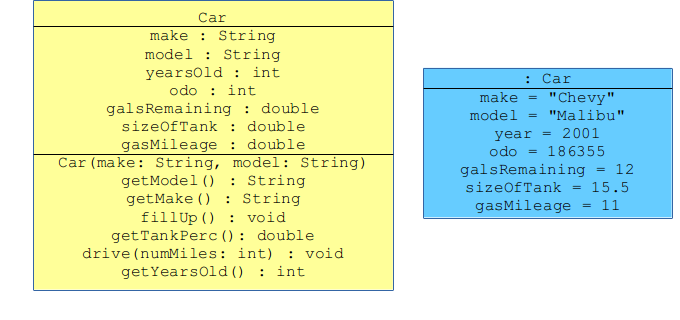
\includegraphics[width=1.0\textwidth]{classObject.pdf}   % 650x350
\caption{A class (left) and an object in UML.}
\label{fig:classObject}
\end{figure}

\subsection{Classes in UML: the first two compartments}

\index{capitalization}
Let's look at the class in detail. In the top box is its name; so far so good.
One thing to point out, though, is that in Java, \textit{the names of all
classes are \underline{capitalized}.} Don't ever violate this rule, for
convention's and confusion's sake!

\index{instance variables (inst vars)}
The second compartment has the class's \textbf{instance variables}. You'll
hear people use other terms for these like like ``member variables'' and even
``class variables,'' but I strongly prefer instance variables (or ``inst
vars'' for short) and here's why: \textit{every instance of a class has its
own copy of its instance variables.} This truth is absolutely fundamental to
OOP, and it's worth re-reading that sentence again and again until it's part
of your core being. Declaring a plain-ol' variable like ``\texttt{int x;}''
creates a single storage location in which a value can be stored. But
declaring an \textit{instance} variable is a far-reaching choice that destines
every \texttt{Car} (or whatever) that will come about in the future to have
its own copy of that variable. It's our way of defining the very structure of
Cars in perpetuity.

One slight headache is that the UML syntax differs from Java's a bit: instead
of listing the variable's type and then its name, we reverse them, we use
a colon instead of a space, and we omit the semicolon. Otherwise, it's pretty
straightforward to interpret that second compartment.

\index{class variable}
\index{underlined}
\index{car@\texttt{Car}}
\index{static@\texttt{static}}
By the way, one important piece of syntax in that second compartment is an
\underline{underline}. If an inst var is underlined, then it actually isn't an
``instance variable'' after all: it's a \textbf{class variable}. This means
that \textit{there's only one shared variable for the entire class, rather
than a different variable for each object.} In Figure~\ref{fig:classObject},
the integer \texttt{num} variable is the only underlined one. So even though
every \texttt{Car} has its own \texttt{make}, \texttt{model},
\texttt{odo}meter reading, \textit{etc.}, they all share one \texttt{num}
(which presumably represents the total number of \texttt{Car} objects
instantiated so far.) This makes sense, since after all such a variable is not
specific to a certain \texttt{Car}. We'll see that in Java, class variables
are created by using the ``\texttt{static}'' keyword where the variable is
declared.

\subsection{Classes in UML: the third compartment}

\index{method}
\index{member function}
The third compartment isn't much harder: it contains the \textbf{methods} for
the class. Like everything it seems, programmers have multiple terms for these
two: they're called \textbf{member functions} or \textbf{class functions} on
occasion. We'll stick with \textbf{method}.

\subsubsection{Functions vs. methods}

\index{function}
The crucial distinction between a method and a regular ol' Joe function is
this: while you can simply call a function to trigger it, you must call a
method \textit{on an object}. In the example, we have a \texttt{fillUp()}
method defined on the \texttt{Car} class. Since it's not an ordinary function,
but rather an OO method, we must call it on a particular instance of a
\texttt{Car}. In Java code, this does \textit{not} work:

\begin{verbatim}
    fillUp();        // NOPE
\end{verbatim}

nor does this:

\begin{verbatim}
    Car.fillUp();    // NOPE
\end{verbatim}

Instead, one must call \texttt{fillUp()} like this:

\begin{verbatim}
    johnsMercedes.fillUp();     // Correct!
\end{verbatim}

where \texttt{johnsMercedes} is the name of a valid \texttt{Car} object,
previously instantiated.

Beginners sometimes view this as a syntactic nuisance. It is not. It is
fundamental to what your code \textit{means}. Conceptually, it makes sense to
have a particular car, and to fill it up. It does \textit{not} make sense to
say ``hey universe, fill up cars'' (which is what ``\texttt{fillUp()}'' seems to
say) nor to say ``hey Cars-in-general, fill yourself up'' (which is what
``\texttt{Car.fillUp()}'' seems to say).

\index{capitalized}
By the way, notice in the example I just gave, \texttt{johnsMercedes} is
\textit{not} capitalized. (The capital ``\texttt{M}'' in the middle doesn't
count; that's just an artifact of CamelCase, which is a way of making multiple
words easier to read.) This is \textit{always} true: in Java, object names
should always begin with a lower-case letter.

Back to the third compartment. You can probably tell that the stuff inside the
parentheses is arguments to the respective methods, with the same
name-first-then-type colon-syntax, and you can probably tell that after the
closing parenthesis, you have the return type of the function. All of this
looks vaguely Java-like, and that's because even though a UML diagram is
technically programming-language-independent, language-specific things like
\texttt{int} and \texttt{String} can't help but creep in in practice. Our
thoughts betray us.

\subsubsection{Various ``special'' methods}
\label{page:instantiateConstructor}

\index{constructor}
\index{void@\texttt{void}}
A few of those methods are worthy of special note. The first one listed,
called simply ``\texttt{Car}'', is a very special kind of method called a
\textbf{constructor} which we'll be talking about a lot. Here's an iron-clad
rule which is fundamental to much that follows: \textit{whenever an object is
instantiated, one of its class's constructors is called.} This happens
automatically; it's not something we have to do ourselves. (Java's syntax for
this, as we'll see, makes it kind of look like we're calling the constructor
ourselves, which is a mixed blessing.) In Java, there are two things that
``make'' a method a constructor: (1) it must have exactly the same name as the
class, and (2) it must have \textit{no} return type. (Note that ``no'' return
type is not the same as a \texttt{void} return type! I mean \textit{no return
type at all.}\footnote{If you mistakenly include a \texttt{void} before your
constructor when you write the code, it is officially no longer a constructor!
It's now just an ordinary method -- weirdly named the same as the name of the
class it's in -- which will not be automatically invoked at instantiation time
as a constructor should. I once had a nasty bug at the eleventh hour of a
software release because of this exact issue.})

By the way, just as a class can have multiple methods with the same name as
long as those methods have different argument lists, so it can have multiple
constructors subject to the same conditions. This is a very common practice,
although in this first example we have only one \texttt{Car} constructor.

\index{underlined}
\index{numCars@\texttt{numCars()}}
Also, just as in the second compartment, an \underline{underline} indicates
that the method ``goes with the whole class, not with each object.'' And just
as before, this implies the use of the \texttt{static} keyword. A
\texttt{static} method is essentially a function: \textit{i.e.}, you
\textit{don't} call it on an object. Instead, you just call it \textit{on the
class itself.} In the example above, \texttt{numCars()} method is
\texttt{static}, which means that you could write ``\texttt{Cars.numCars()}''
to retrieve the number of \texttt{Car} objects that have been instantiated to
that point. Static methods are quite rare, but they do arise occasionally, and
are always indicated with an underline.

\index{getter}
\index{setter}
\index{mutator}
\index{accessor}
The other methods I'll draw your attention to are the ones that begin with
``\texttt{get}''. People call these methods ``\textbf{getters},'' and all they
normally do is return the value of the instance variable in question. Often
one also has ``\texttt{set}'' methods to set the values of inst vars, although
our example doesn't have any of those. Btw, some people also call getters and
setters \textbf{accessors}, and sometimes specifically call setters
``\textbf{mutators},'' a term which always made me chuckle.

\subsection{Objects in UML}

\index{object}
\index{state}
Now let's examine the blue box in Figure~\ref{fig:classObject}, which
represents an object rather than a class. It has only two compartments, not
three. That's because there's no need (in most OO languages) to say anything
about an object's methods when focusing on the object: after all, the methods
are simply defined by the class, and are common to all instances of that
class. It is important, however, to specify the current \textbf{state} of the
object, which means the current values of all its instance variables. In the
picture, you can see that there is a \texttt{Car} object in memory
representing an old Chevy Malibu with a zillion miles on it and other
suboptimal features.

\index{names}
Perhaps the strangest thing about a UML object is the top compartment. Notice
that it says ``\texttt{:~Car}'' (``colon-Car''), which is not a typo. Here's
the sitch. The top compartment of a \textit{class} has the class's name, since
that's all there is to say about it. The top compartment of an \textit{object},
meanwhile, has the \textit{object's} name, followed by a colon and then its
class. Just like we said ``\texttt{make :~String}'' earlier, so here we can
say ``\texttt{johnsMercedes :~Car}''. Why, then, is
Figure~\ref{fig:classObject} missing the name before the colon? Because we've
chosen \textit{not to name this object in the diagram.} It's just ``a Car''
with certain properties, not a named Car. This may seem odd, but in fact 99\%
of the time we will do exactly this. And that's because bizarrely,
\textit{objects don't have names in Java}, even though it may seem at first
that they do.

More on that later. For now, just accept the fact that UML diagrams can depict
objects, and normally we don't choose to specify the object's name -- only its
type and its instance variable values.


\subsection{The value of ``design''}

\index{design}
\index{class diagram}
\index{blueprint}
Before we move on to implementation, take a step back for a moment and
consider the \textit{information} contained in that
Figure~\ref{fig:classObject}.

Suppose you were given the job to write a car maintenance tracking program,
and you were getting started figuring out how to accomplish that. I think
you'll agree that if someone handed you that diagram, it would be valuable
indeed. There's no code in it \textit{per se}, but a great deal of the work
has already been done for you! You already know what to name your class, the
names and types of all its constituent variables, and what methods its objects
should support. With that diagram alone, I'd say 70\% of the work has been
done. All it takes now is to convert that diagram into Java (or whatever
language you're working with), and flesh out the methods to do the right
thing. But the overall blueprint communicates a ton of information about
decisions that have already been made. Your structure is defined, and now you
just need to bust out a hammer and some nails.


\section{Classes in Java}

\index{class@\texttt{class}}
\index{java file@\texttt{.java} file}
\index{vim@\texttt{vim}}
In Java, every class is in its own file\footnote{Technically there can be
some exceptions to this, but don't worry about them now.} named the same as
the name of the class (including the capital letter) with a \texttt{.java}
extension. Operationally, we can use \texttt{vim} to create it and edit it:

\begin{verbatim}
$ vim  Car.java
\end{verbatim}

\index{package@\texttt{package} statement}
\index{import@\texttt{import} statement}
% TODO: *Do* we actually talk about "package statements" later?
The skeleton of any class file -- after the \texttt{package} and
\texttt{import} statements we'll talk about later -- is the class definition,
with curly braces:

\begin{Verbatim}[samepage=true,fontsize=\footnotesize,frame=single]
class Car {
    
}
\end{Verbatim}

\index{public@\texttt{public}}
You may be used to putting the word ``\texttt{public}'' before the word
\texttt{class} here. For now, we won't do this, and I'll encourage you to
ditch the habit of making classes \texttt{public} by knee-jerk reaction. As
we'll learn, you want to lean towards making things ``as private as possible''
until you have reason to do otherwise.

\subsection{Instance variables in Java}

\index{instance variables (inst vars)}
Instance variables go directly inside the class definition, and outside of any
method:

\begin{Verbatim}[samepage=true,fontsize=\footnotesize,frame=single]
class Car {
    String make, model;
    int yearsOld;
    int odo;
    double galsRemaining;
    double sizeOfTank;
    double gasMileage;    
}
\end{Verbatim}

\index{private@\texttt{private}}
You may be used to seeing the word ``\texttt{private}'' before each instance
variable, and I do applaud that practice. More on that later. For now, we'll
leave it off just because it's not necessary to compile. Realize that it's not
the word \texttt{private} that makes something an instance variable; rather,
it's the fact that it's defined directly inside the class, rather than within
a method.

\subsection{Constructors in Java}

\index{constructor}
Next on the diagram is our constructor. We put in the boilerplate to get us
started:

\begin{Verbatim}[samepage=true,fontsize=\footnotesize,frame=single]
class Car {
    ...

    Car(String make, String model) {

    }
}
\end{Verbatim}

and now for the first time we have to actually think.

A constructor, as I said, is automatically called whenever an object comes
into existence. This is our ``hook'' to set up the object for success when
methods are called on it later. Think of it this way: your constructor is
called whenever a new object is about to come off the assembly line and enter
the real world. Your job in the constructor is to do everything necessary to
make sure it's ready for prime time.

Often this will involve initializing the instance variables to reasonable
values. Sometimes it will include other things, like registering its existence
in some global repository of objects, or initializing a connection to a
network, or writing itself to a database. The key question to ask yourself is,
``what do I need to do to ensure this object is `legit' and doesn't break
anything when it's being used?''

\subsection{Analyze \texttt{this}}

\index{this@\texttt{this}}
In our case, initializing the instance variables are all we need to do in the
constructor. First, let's set the object's \texttt{make} and \texttt{model} to
what was passed:

\begin{Verbatim}[samepage=true,fontsize=\footnotesize,frame=single]
class Car {
    ...

    Car(String make, String model) {
        this.make = make;
        this.model = model;
    }
}
\end{Verbatim}
\normalsize

\index{Gosling, James}
If this is the first time you've seen the odd word ``\texttt{this}'' in a
program, have a good chuckle. What a weird word choice! But Gosling \&
Co.~chose this word to denote a central OO programming concept. The word
``\texttt{this}'' means one of two different things, and they both need to be
memorized:

\begin{enumerate}
\large
\itemsep.1em
\item Inside a \textit{constructor}, ``\texttt{this}'' means ``the object that is
currently being instantiated.''
\item Inside a \textit{method}, ``\texttt{this}'' means ``the object the
method was called on.''
\item[-.] (Anywhere else, ``\texttt{this}'' is illegal.)
\normalsize
\end{enumerate}

It's weird and meta and self-referential, but it's also necessary. There are
times when we need to have a name for ``the very object I'm `in' right now,''
and ``\texttt{this}'' is our (awkward) name to refer to that.

So in our constructor, when we say ``\texttt{this.make}'' we mean ``the
\texttt{make} instance variable of this very object that is in the process of
being birthed.'' We set that to the \texttt{make} argument that was passed to
the constructor. Ditto with \texttt{model}. Oftentimes, using \texttt{this} is
optional, but in the present case it's required because we named our argument
the same as the instance variable, and there has to be a way to distinguish
between the two.

\index{initialization}
Now for our other inst vars. Some of them make sense to be set to zero:

\begin{Verbatim}[samepage=true,fontsize=\footnotesize,frame=single]
class Car {
    ...
    Car(String make, String model) {
        this.make = make;
        this.model = model;
        this.yearsOld = 0;
        this.odo = 0;
        this.galsRemaining = 0.0;
    }
}
\end{Verbatim}

since brand new cars are in fact zero years old, have a 000000 odometer, and
have no gas in their tank (maybe). Zero values for the other two don't make
sense, however; brand new cars still have a gas tank of a certain size, and
they certainly get more than 0 mpg. For this example, I'm going to go with a
very limited notion of automotive properties:

\begin{Verbatim}[samepage=true,fontsize=\footnotesize,frame=single]
class Car {
    ...
    Car(String make, String model) {
        this.make = make;
        this.model = model;
        this.yearsOld = 0;
        this.odo = 0;
        this.galsRemaining = 0.0;
        
        if (make.equals("Chevy") || make.equals("GM")) {
            sizeOfTank = 21;
        } else {
            sizeOfTank = 13;
        }
        if (make.equals("Chevy") && model.equals("Malibu")) {
            gasMileage = 3;
        } else {
            gasMileage = 24;
        }
    }
}
\end{Verbatim}

I'm totally not bitter about my car's gas mileage, by the way.

\subsection{Methods in Java}

The other methods follow a similar syntactic pattern. But it's super important
to keep this truth in the front of your mind: \textit{because they are methods
(not functions), they are called \underline{on an object.}} That means that
you can refer to instance variables inside of them -- and when you do, you're
talking about \textit{the instance variables of the object the method was
called on.} Put another way, you're talking about the instance variables of
\texttt{this}.

\subsubsection{``Client code'' and thinking reactively}

When you write methods in an OO program, you have to think reactively, not
proactively. What I mean is this. When you write a procedural, old school
program, you're the one in control. You set the agenda. In your
\texttt{main()} you say, ``first do this, then do that; create these three
variables, perform a computation, and then print the result.''

We all learned how to program this way. But in OO, you kind of have to think
backwards from that. Writing a method isn't like calling it; instead of giving
orders, you're providing a service to whoever called you. So when you write a
method, you have to think, ``okay, some other part of the code is now calling
me, for reasons of its own. What do I do in response to that?''

\index{client code}
Our term for ``that other part of the code that is now calling me'' is
\textbf{client code} (or sometimes just ``a \textbf{client}.'') The word
``client'' is used in a lot of different ways in high-tech, but here we just
mean ``the code that wants to use a particular object.'' The word connotes a
respected customer, whom we want to treat well. Very well, some client code
calls one of our methods. How should we react?

\index{state}
Often we'll react by updating the object's \textbf{state} to reflect what
should happen to it as a result of the method being called. Sometimes we'll
produce (return) a value that is stored by the object in question or
computed on the fly. Other times we'll trigger some side effect, like printing
to the screen, writing to a database, or calling some \textit{other} method(s)
on the same or a different object.

\index{implement}
\index{fillUp@\texttt{.fillUp()}}
This is best seen through examples. Let's implement\footnote{The verb
\textbf{to implement} means ``to take a design and actually build it out.'' It
is a synonym for the verb \textbf{to code}.} the \texttt{.fillUp()} method
first. Don't think about Java; think about cars. If I fill up a car, what
happens?

Does the make or model or mileage change? Of course not: the amount of gas in
the tank does. And ``fill 'er up'' means to raise it to its maximum. The
correct implementation of \texttt{.fillUp()}, then, is simply:

\begin{Verbatim}[samepage=true,fontsize=\scriptsize,frame=single]
class Car {
    ...
    void fillUp() {
        galsRemaining = sizeOfTank;
    }
}
\end{Verbatim}

We could equally well have written this as:

\begin{Verbatim}[samepage=true,fontsize=\scriptsize,frame=single]
class Car {
    ...
    void fillUp() {
        this.galsRemaining = this.sizeOfTank;
    }
}
\end{Verbatim}

to make it explicit that we're talking about two instance variables here, and
assigning the value of one to the other. It's a matter of style.

In the same vein, we ask ourselves, ``suppose some client code asks me what
percentage full my tank is. What answer do I give them?'' The proper response
involves these same two inst vars and a little math:

\begin{Verbatim}[samepage=true,fontsize=\scriptsize,frame=single]
class Car {
    ...
    double getTankPerc() {
        return galsRemaining / sizeOfTank * 100;
    }
}
\end{Verbatim}

I chose to omit \texttt{this}, but again it's a personal choice.

Some methods are no-brainers:

\begin{Verbatim}[samepage=true,fontsize=\scriptsize,frame=single]
class Car {
    ...
    String getModel() {
        return model;
    }
}
\end{Verbatim}

If a client asks me what my model is, I tell them my model, duh. The same is
true for the other accessor methods.

\index{drive@\texttt{.drive()}}
Finally, what if a client instructs me to drive $n$ miles? How should my
internal state be adjusted to reflect that?

This is the most difficult one, and again it requires you to think about cars
rather than about Java. Mentally run through the variables we've chosen to
represent a car, and ask yourself which ones need to change, and how? You'll
realize that the odometer and the gas tank level are the two we need to
modify. When someone drives a car $n$ miles, the odometer needs to increase by
$n$ miles (else it ain't legal); also, the gas tank needs to be reduced by
$\frac{n}{m}$ gallons, where $m$ is the car's gas mileage in mpg. So here we
go:

\begin{Verbatim}[samepage=true,fontsize=\footnotesize,frame=single]
class Car {
    ...
    void drive(int numMiles) {
        double galsBurned = numMiles / this.gasMileage;
        this.galsRemaining = this.galsRemaining - galsBurned;
        this.odo += numMiles;
    }
}
\end{Verbatim}

This time, I did include the \texttt{this}'s where appropriate, since we also
have a couple of local variables involved and I wanted to be explicit. Our
math is a mix of function parameters, temporary variables, and permanent
attributes of the \texttt{Car}.


\section{Objects in Java}

\index{object}
We've now coded a class from the ground up (the complete code listing is in
Figure~\ref{fig:carClassCodePreExceptions}.) We did this so clients can
instantiate objects of that type and do something with them. Let's make a
simple \texttt{main()} method to do just that.

You'd be surprised how many beginning programmers try to drive 23 miles like
this:

\begin{Verbatim}[samepage=true,fontsize=\scriptsize,frame=single]
    public static void main(String args[]) {
        drive(23);    // WRONG!
    }
\end{Verbatim}

or this:

\begin{Verbatim}[samepage=true,fontsize=\scriptsize,frame=single]
    public static void main(String args[]) {
        Car.drive(23);    // equally WRONG!
    }
\end{Verbatim}

Yes you'll get compiler errors, but those errors reflect a deeper and more
fundamental misunderstanding. In OOP, you have to call a method \textit{on an
object}. Conceptually, nothing else makes sense. In real life you don't
``drive in general,'' and you don't ask ``automobiles in general'' to drive
you places. Instead, you have to drive \textit{a particular car} somewhere.
Here's how:

\begin{Verbatim}[samepage=true,fontsize=\scriptsize,frame=single]
    public static void main(String args[]) {
        Car minivan = new Car("Toyota","Sienna");
        minivan.drive(23);    // correct!
    }
\end{Verbatim}

\index{new@\texttt{new}}
\index{instantiate}
The keyword ``\texttt{new}'' is utterly crucial here. In Java, \textit{the only
way to instantiate an object is to use \texttt{new}}. It causes a fresh object
of the appropriate type to spring into existence, complete with memory to hold
its instance variables. And the appropriate constructor is called, of course,
to set that object up for prime time.

We got errors before because we didn't even \textit{have} a car to do anything
with. There was no memory set aside, no constructor called to set up the
object, nothing. We tried a shortcut, and that was madness. But now that we
know how to instantiate objects, we can do so to several and create a whole
new world, as in Figure~\ref{fig:wholeNewWorld} on
p.~\pageref{fig:wholeNewWorld}. All the code in that figure is legit, and
shows that our \texttt{Car} class has uses.

\begin{figure}[h]
\centering
\begin{Verbatim}[samepage=true,fontsize=\footnotesize,frame=single]
    public static void main(String args[]) {

        // The archaic Davies family vehicles
        Car minivan = new Car("Toyota","Sienna");
        minivan.setYear(2002);
        Car stephensLemon = new Car("Chevy","Malibu");
        minivan.setYear(2001);

        // Grammy lives in Colorado
        Car grammysCar = new Car("Lexus","ES");
        grammysCar.setYear(2018);

        // Caravan to Disneyworld -- whoo-hoo!  (Grammy's meeting us there.)
        minivan.fillUp();
        minivan.drive(500);
        stephensLemon.fillUp();
        stephensLemon.drive(500);
        System.out.println("The van is " + minivan.getTankPerc() + 
            "% full, while the chevy is " + stephensLemon.getTankPerc() +
            "% full.");
        grammysCar.drive(1899);  // a long way from Colorado
    }
\end{Verbatim}
\caption{A client \texttt{main()} program that uses the \texttt{Car} class.}
\label{fig:wholeNewWorld}
\end{figure}


\subsection{Printing an object}

One last thing before we bring this chapter to a close. Suppose we're
debugging our program, and we want to print out the values of various
variables to help us hunt down an error. Printing an \texttt{int} or other
standard type is straightforward:

\begin{Verbatim}[samepage=true,fontsize=\scriptsize,frame=single]
    int numEnchiladas = 3;
    System.out.println("The number of enchiladas is: " + numEnchiladas + ".");
\end{Verbatim}

and will produce a message like ``\texttt{The number of enchiladas is 3.}''
What happens, though, if we print out an \textit{object}, like a \texttt{Car}?
How can such a complex entity be reduced to a string of text?

Heck, let's try it:

\begin{Verbatim}[samepage=true,fontsize=\scriptsize,frame=single]
    Car porsche = new Car("Porsche","Carrera");
    porsche.setYearsOld(2);
    System.out.println("My car is: " + porsche + ".");
\end{Verbatim}

The output we get is:

\begin{verbatim}
   My car is: Car@4aa298b7.
\end{verbatim}

Whoa. The word ``\texttt{Car}'' is perhaps not surprising, but what's the rest
of that gunk?

\index{memory address}
It turns out that Java's default way of rendering an object as a
\texttt{String} is to concatenate the name of the class, an ``at'' sign,
followed by \textit{the memory address} in which it is stored. We'll talk much
more about memory in the next chapter. For now, just think of the memory
address as a unique number\footnote{Yes, it is indeed a number, despite the
fact that it has letters in it like '\texttt{a}' and '\texttt{b}'. It's
printed here in \textbf{hexadecimal}, which is a base-16 number system instead
of the base-10 system non-computer-science humans use.} that identifies the
object, like an SSN.

\begin{samepage}
\label{pg:toString}
\index{override}
\index{toString@\texttt{.toString()}}
The cool thing is, we can \textbf{override} this functionality at will, and
change the way \texttt{Car}s will be printed. Check it out. Create a method in
the \texttt{Car} class called \texttt{.toString()}. It must:

\begin{compactenum}
\itemsep.1em
\item be called exactly ``\texttt{.toString()}''.
\item take no argument.
\item return a \texttt{String}.
\index{public@\texttt{public}}
\item have the word \texttt{public} immediately before the return type. (We'll
talk a lot about what \texttt{public} means in future chapters. For now, it just has to
be there.)
\end{compactenum}
\end{samepage}

Here's one:

\begin{Verbatim}[samepage=true,fontsize=\scriptsize,frame=single]
    public String toString() {
        return "a " + yearsOld + "-year-old " + make + " " + model;
    }
\end{Verbatim}

We're assembling various aspects of the vehicle into a sensible, readable
string. Now, when we run \textit{the same code} as above, our output is this:

\begin{verbatim}
   My car is: a 2-year-old Porsche Carrera.
\end{verbatim}

Notice that we didn't explicitly ever call \texttt{.toString()}! Instead, we
just used a \texttt{Car} object in a context in which a \texttt{String} was
required, and Java faithfully called our method instead of the one that
generated the memory address. Pretty cool.

\texttt{inheritance}
This is actually our first foray into a really deep and powerful technique
called ``inheritance,'' about which much more will come in later chapters. For
now, just grasp the idea that Java lets us override its general behavior for
specific kinds of objects, which gives us tremendous power and flexibility.

\begin{figure}
\begin{Verbatim}[fontsize=\scriptsize,frame=single]
class Car {
    String make, model;
    int yearsOld, odo;
    double galsRemaining, sizeOfTank, gasMileage;

    Car(String make, String model) {
        this.make = make;
        this.model = model;
        yearsOld = 0;
        odo = 0;
        galsRemaining = 0;
        if (make.equals("Chevy") || make.equals("GM")) {
            sizeOfTank = 21;
        } else {
            sizeOfTank = 13;
        }
        if (make.equals("Chevy") && model.equals("Malibu")) {
            gasMileage = 3;
        } else {
            gasMileage = 24;
        }
    }

    public String toString() {
        return "a " + yearsOld + "-year-old " + make + " " + model;
    }

    String getMake() { return make; }

    String getModel() { return model; }

    int getYearsOld() { return yearsOld; }

    void setYearsOld(int x) { yearsOld = x; }

    void fillUp() {
        this.galsRemaining = this.sizeOfTank;
    }

    double getTankPerc() {
        double perc = galsRemaining / sizeOfTank * 100;
        return perc;
    }

    void drive(int numMiles) {
        double galsBurned = numMiles / gasMileage;
        galsRemaining = galsRemaining - galsBurned;
        odo += numMiles;
    }
}
\end{Verbatim}
\caption{A complete Java implementation of the \texttt{Car} class.}
\label{fig:carClassCodePreExceptions}
\end{figure}


\chapter{Memory matters}
\label{ch:memoryMatters}

This chapter is near and dear to my heart. The concepts here are vastly
undertaught by computer science educators today, and yet they are at the
epicenter of most intermediate students' understanding (or misunderstanding).
A failure to master this material slaps a hard ceiling on what you can
accomplish as a programmer. Successfully mastering it is the key to the next
level.

The key idea is that there are two ways of looking at a computer program. One
is to look at the static lines of code as they are written on a screen or on
paper. This is how novices think about programs: they look at the lines of
code, and ask themselves whether lines need to be added, removed, changed, or
moved.

\index{memory}
The other way is to think about what happens to the computer's \textbf{memory}
as the program runs, and how its variables and structure change as the program
unfolds. Whether they realize it or not, this is how all proficient
programmers think. It turns out that \textbf{the ``purpose'' of almost any line
of code is to change the contents of memory in a particular way.} The name of
the game is recognizing what impact on memory each line of code has -- and
conversely, what line of code is required to make a particular change to
memory.

\section{Memory diagrams}

\index{memory diagram}
\index{snapshot}
The focal point of this chapter will be the \textbf{memory diagram}, which
incorporates the UML object representations we discussed in
section~\ref{sec:UMLclasses}. A memory diagram depicts the contents of the
computer's memory at a \textit{snapshot in time.} At any given moment, as a
program is running, you could say ``Freeze!''\ and look at the memory diagram.
You'd see the exact state of the system at that moment.

\subsection{The stack and the heap}

\index{stack@the stack}
\index{heap@the heap}
\index{memory!statically-allocated}
\index{memory!dynamically-allocated}

A program's memory, it turns out, is divided into two realms with funny names:
``\textbf{the stack}'' and ``\textbf{the heap}.'' It is vital to understand the
difference between the two, and which one is used for what. The stack contains
\textbf{statically-allocated}, and the heap \textbf{dynamically-allocated},
memory. We'll unpack what all this means, but first let me show you a full list
of differences:

\small
\vspace{.2in}
\begin{tabular}{c|c}
\textbf{stack} & \textbf{heap} \\
\hline
statically-allocated & dynamically-allocated \\
\index{names}
holds named things & holds unnamed things \\
holds primitive types and references & holds objects\footnote{This is
true in Java, but C++ permits programmers to store objects on the
\textit{stack} as well as the heap. I will argue that's universally dumb, and
it's a large part of what makes programming in C++ difficult: you have to
account for that occurrence with a ton of tedious and error-prone
bookkeeping.} \\
\index{lifespan}
items have limited lifespan & items have unlimited lifespan\footnote{Not
completely unlimited, but things on the heap stick around as long as they're
needed, rather than evaporating at the end of their current function.} \\
\end{tabular}
\vspace{.2in}
\normalsize

This is best understood by example, and in fact can be illustrated with just a
small function:

\begin{Verbatim}[fontsize=\small,samepage=true,frame=single]
void illustration() {
    int year = 2018;
    Car minivan = new Car("Toyota","Sienna");
}
\end{Verbatim}

This teensy function, when it runs, produces memory contents as depicted in
Figure~\ref{fig:stackHeap1}. Let's go through it carefully.

\begin{figure}[ht]   % 590x220
\centering
\includegraphics[width=1\textwidth]{stackHeap1.pdf}
\caption{The stack and the heap.}
\label{fig:stackHeap1}
\end{figure}

\index{primitive type}
The first line of \texttt{illustration()} creates a simple integer variable
and sets it equal to 2018. Since an \texttt{int} is a \textbf{primitive
type}\footnote{If you've never heard this lingo, a ``primitive type'' is one of
the very basic lower-case Java variable types, like \texttt{int},
\texttt{double}, or \texttt{boolean}. Importantly, a primitive type is
\textit{not} an object.}, it is stored on the stack. ``On'' the stack should
make you think of layering items vertically on a surface. Before this line of
code executed, nothing existed in the program's memory at all, so the stack
was nothing but a bare floor (think of it as a horizontal line). Our first
variable goes right on top of that floor.

\index{reference variable}
\index{variable, reference}
There's a ton packed into that second line of code, so hold on to your seats.
The first thing to realize is that \textit{it encompasses both stack and
heap.} We have a named \textbf{reference variable} called \texttt{minivan},
which, as with all named things, goes on the stack (right on top of
\texttt{year}). A ``reference variable'' means a variable that has the ability
to reference (or ``refer to,'' or ``point to'') an object. However, the object
itself is created in the heap, because in Java that's where all objects live.
The word \texttt{new} is a ``heap word'': using it is the only way to make an
object at all, and therefore, the only way to make something on the heap.
Finally, to carry out the equals sign (``\texttt{=}'') in that line of code, we
draw an arrow from \texttt{minivan} to the object to indicate that's what it's
currently referring to.

%\subsubsection{(...a brief commercial...)}
%
%Now before we go any further, I want to \textit{\textbf{implore}} you that
%\textit{this stuff does actually matter.} It's tempting at this point to think
%that all this gibberish about stack and heap and whether something's on the
%left or right side of a diagram is irrelevant.  Nothing could be further from
%the truth. As soon as our example gets even moderately complicated, you will
%absolutely get the wrong answer if you conflate or confuse the two memory
%realms, or fail to keep their contents utterly in sync. Trust me on this.
%
%\subsubsection{(...okay, back to work...)}

\index{names}
Okay, now a head-scratcher. Look at Figure~\ref{fig:stackHeap1} again. What
would you answer if I asked you, ``what's the \textit{name} of that blue
object?''

If you're like 99\% of novice programmers (including myself, long ago), you
would confidently answer, ``\texttt{minivan}. Its name is \texttt{minivan}.''
That seems to make perfect sense. But unfortunately it is \textit{wrong}. The
truth is that \textit{the object has no name.}

Again, you may think I'm being pedantic. Let me demonstrate why I'm not.
Suppose we expanded our previous code with four more lines, as depicted in
Figure~\ref{fig:additionalCode}. Study it carefully.

\begin{figure}
\begin{Verbatim}[fontsize=\small,samepage=true,frame=single]
void illustration() {
    ...
    Car other = new Car("Ferrari","F355");
    Car t = minivan;
    minivan = other;
    other = t;
}
\end{Verbatim}
\caption{(Continuing the previous example.)}
\label{fig:additionalCode}
\end{figure}

\index{car@\texttt{Car}}
Let's deal with the first two of these lines. The first one creates a new
reference variable called \texttt{other} on the stack, and points it to a
brand new \texttt{Car} object (unrelated to our Toyota Sienna) in the heap.
Notice that unlike with the stack, I didn't carefully put the new \texttt{Car}
exactly on top of the first one. Instead, I just threw it in there helter
skelter. This is how the heap works, and in fact why it's called a ``heap'':
it's a disorganized mess of stuff that comes and goes in response to the
program's unpredictable needs. The stack is as tidy as the Library of
Congress; the heap is a teenage boy's room. Seems weird, but it turns out
things have to be that way.

The second line creates a new stack variable called \texttt{t} but
emphatically does \textit{not} create a new \texttt{Car} object. Let that sink
in deeply. Many programmers, upon seeing a line begin with ``\texttt{Car t =
...} would naturally assume that line is making a new \texttt{Car}. But it's
actually only creating another variable that has the \textit{potential} to
refer to a \texttt{Car}. And in fact, after the equals sign, we do point it to
a \texttt{Car}...but one of the ones we've already instantiated (namely, the
Sienna).

The result of executing these two lines is shown in
Figure~\ref{fig:stackHeap2}. Stare very carefully at that figure and mull over
each box and line. We have four named variables, three of which are of type
\texttt{Car}, and yet there are only \textit{two} \texttt{Car} objects because
we only executed two \texttt{new}'s. And two of our named variables --
\texttt{t} and \texttt{minivan} -- are pointing to \textit{the same object}.
This turns out to be okay. We'll have multiple references to the same object
all the time, and it's entirely healthy. What's critical not to miss is that
\texttt{t} and \texttt{minivan} are not referring to identical copies of the
\texttt{Car}, but literally \textit{the same \texttt{Car}}. If we were to
change the state of \texttt{t}'s \texttt{Car} by, say, increasing its odometer
instance variable, \texttt{minivan} would instantly experience the same
change. And that's because they \textit{are} the same. 

\begin{figure}
\centering
\includegraphics[width=1\textwidth]{stackHeap2.pdf}   % 620x230
\caption{After executing the first two lines of code
Figure~\ref{fig:additionalCode}.}
\label{fig:stackHeap2}
\end{figure}


Okay, now the punchline of this whole example. I'm going to complete the
bait-and-switch, just to prove I was correct back when I said ``the name of
that first blue box is \textit{not} \texttt{minivan}.'' Let's do the
\textit{second} two lines of code in Figure~\ref{fig:additionalCode}:

\begin{Verbatim}[fontsize=\small,samepage=true,frame=single]
    ...
    minivan = other;
    other = t;
\end{Verbatim}

The result of those two operations is to change what the \texttt{other} and
\texttt{minivan} variables are pointing to. Memory now looks like
Figure~\ref{fig:stackHeap3}. And so I ask you again: ``what's the
\textit{name} of that Toyota Sienna object?'' I think you'll agree that
\texttt{minivan} is most certainly \textit{not} its name. Two valid ways to
refer to it are \texttt{t} and \texttt{other}, both of which point to it. But
neither one is its name. Objects simply have no name.

Names are ephemeral, momentary: they're only used temporarily so we can get at
the stuff in the heap, which is ultimately what matters.

\begin{figure}
\centering
\includegraphics[width=1\textwidth]{stackHeap3.pdf}   % 620x230
\caption{Finally, after executing the rest of code
Figure~\ref{fig:additionalCode}.}
\label{fig:stackHeap3}
\end{figure}

\index{lifespan}
Let me conclude this example by explaining what I meant earlier about
``limited lifespans.'' After executing the ``\texttt{other = t;}'' line, we are
done with the function. It's time to return control to whoever called
\texttt{illustration()} in the first place. And at this point, all of our
named variables -- \texttt{t}, \texttt{other}, \texttt{minivan}, and even
\texttt{year} -- cease to exist. Their destiny was only to provide service
during the time that \texttt{illustration()} was being executed. 

But the stuff on the heap lives on after. Long after a function is completed,
the objects it may have created or changed have a presence that will affect
the behavior of other, future functions. In this case, since we weren't passed
any arguments and didn't return anything, our Toyota and Ferrari \textit{will}
actually peacefully go away. But in general there are meaningful, long-term
effects, and in the next section we'll see an example in action.

Most methods are just like this. They create a few named variables so they can
change the contents of the heap in some way, and then clean up their toys
and return with the heap thus changed. That is their \textit{raison d'etre}.
It's a short but happy life.


\section{Calling functions}

\index{function}
One thing our previous example didn't include was calling a function or
method. In this section, we'll see what happens to memory when we do this.
There will probably be a few eye-openers for you.

First, take a look at our code listing (Figure~\ref{fig:functionCode}). We'll
switch from an automotive domain to part of a baseball simulator.

\index{ballplayer@\texttt{Ballplayer}}
\begin{figure}
\centering
\begin{Verbatim}[fontsize=\footnotesize,samepage=true,frame=single]
class Simulator {
    public static void main(String args[]) {
        int year = 2018;
        String greeting = "Play ball!";
        Ballplayer oldGeezer;

        ArrayList yankees = buildDaTeam();
        int rosterSize = yankees.size();
    }

    static ArrayList buildDaTeam() {
        String name = "Yankees";
        int year = 1927;
        ArrayList team = new ArrayList();

        Ballplayer ruth = new Ballplayer("Babe Ruth");
        ruth.setUni(3);
        ruth.setPos("OF");
        Ballplayer gehrig = new Ballplayer("Lou Gehrig");
        ruth.setUni(4);
        ruth.setPos("1B");
        Ballplayer babe = ruth;
        babe.setUni(3);       // (Pointless, as it turns out.)
        babe.setPos("OF");    // (Pointless, as it turns out.)
        team.add(babe);
        team.add(gehrig);
        team.add(ruth);
        
        return team;
    }
}
\end{Verbatim}
\caption{Some code that calls a function.}
\label{fig:functionCode}
\end{figure}

Let's see how the memory diagram emerges line-by-line in response to the code
executing.

First, let's execute the first three lines of \texttt{main()} and
``Freeze!''\ the picture. The result of these lines is shown in
Figure~\ref{fig:bpStackHeap1}. There are three new things here worth
mentioning. First, notice that our \texttt{greeting} variable, although it is
a \texttt{String}-with-a-capital-S and therefore an object, is shown on the
\textit{stack}, just like the \texttt{int year} is. The reason for this is
that Strings are a kind of in-between case (between primitive types and
objects) -- they're neither fish nor fowl. Technically they're objects, but
Java actually treats them somewhat specially, and even has an inline syntax to
create what are actually instances, so it ends up making more sense to treat
them as primitive types on the stack. That's what we'll always do with
\texttt{String}s.

\begin{figure}   % 650x240
\centering
\includegraphics[width=.9\textwidth]{bpStackHeap1.pdf}
\caption{Memory contents after executing the first three lines of
\texttt{main()}.}
\label{fig:bpStackHeap1}
\end{figure}

\subsubsection{Null references and NPEs}

\index{null pointer (or reference)}
\index{null@\texttt{null}}
The next new thing is that bizarre symbol next to \texttt{oldGeezer}.
\textit{Whazzat?} If you look at the code listing, you'll see that we
declare a variable of type \texttt{Ballplayer} named \texttt{oldGeezer}, but
we never set it equal to a \texttt{new} instance, nor to anything else for
that matter. This means that \texttt{oldGeezer}, which as you'll recall is a
``reference variable'' (capable of referring to a \texttt{Ballplayer})
currently refers to \textit{nothing}. In Java, this is called a \textbf{null
reference} (or \textbf{null pointer}) and is indicated with the keyword
\texttt{null}. In fact, this line of code has exactly the same effect as the
one above:

\begin{Verbatim}[fontsize=\small,samepage=true]
    Ballplayer oldGeezer = null;
\end{Verbatim}

Some people prefer to be explicit like this. I don't care either way; just
realize that at this point, if you attempted to call \textit{any} method on
\texttt{oldGeezer}, like:


\begin{Verbatim}[fontsize=\small,samepage=true]
    Ballplayer oldGeezer = null;
    oldGeezer.strikeout();
\end{Verbatim}

\index{NPE (null pointer exception)}
you will then be hit with the most ubiquitous of all Java
run-time errors, the \textbf{null-pointer exception} (or ``\textbf{NPE}''):

\begin{Verbatim}[fontsize=\small,samepage=true]
Exception in thread "main" java.lang.NullPointerException
    at Simulator.main(Simulator.java:5)
\end{Verbatim}

This is quite reasonable behavior, if you think about it. What can Java do if
you try to ``call a method on an object'' but there \textit{is} no such object?
It can only throw up its hands, which it does here.

Remember: an NPE means \textit{you tried to call a method on an object, but
the variable name you called it on wasn't actually an object; it was}
\texttt{null}. The way to diagnose an NPE is to look at the line number it
gives you, and find the dot (``\texttt{.}'') (or dots) on that line. The
variable or expression to the \textit{left} of one of those dots is an
uninitialized, null reference. Guaranteed.

\subsubsection{Stack frames}

\index{stack frame}
\index{recursion}
The last new thing in Figure~\ref{fig:bpStackHeap1} is easy to miss: it's the
word \texttt{main()} off on the left-hand side of the diagram. What this means
is that \textit{all the variables to the right of it ``belong'' to the
\texttt{main()} function.} This group of variables, which goes with a
particular call to a function\footnote{Note carefully that a stack frame is
associated with each \textbf{\textit{call}} to a function, not each function.
This may seem pedantic, and it is...until we consider \textbf{recursion}. A
recursive function will call itself, which will call itself, which will call
itself...many times. \textit{Each call} to the function generates its own
stack frame, which is separate from all the others. This is how recursive
functions are able to work without clobbering the values of the variables
contained in previous, still-active calls.}, is called a \textbf{stack frame}.
The way a program works is this: every time a function is called, a new stack
frame is ``pushed'' on top of the stack (above a horizontal line that we'll
draw.) While we're in the function, \textit{Java can only see the variables in
that current stack frame.} The ones in \texttt{main()}'s stack frame, or any
other stack frame for currently-in-progress functions, are safely nestled away
to be resumed later, but they are not immediately available to the program.

This is exactly how it should be. If we call a function \texttt{foo()} from
within a function \texttt{bar()}, control transfers to \texttt{foo()}. Now how
could \texttt{foo()} possibly refer to \texttt{bar()}'s variables? Heck,
whoever wrote the code for \texttt{foo()} didn't even know it would be
\textit{called} from \texttt{bar()}! Any other function could have called it
just as well, in which case \texttt{bar()}'s variables wouldn't even exist.
All we know for sure is that \texttt{foo()} was called from ``somewhere,'' and
thus must work no matter what the context. If Java allowed us to talk about
variables in another stack frame, our function would instantly become
non-reusable; it would only make sense if called from some specific other
function. And that defeats most of the purpose of even having a function.

Okay, now the big moment. We run this line:

\index{buildDaTeam@\texttt{buildDaTeam()}}
\begin{Verbatim}[fontsize=\small,samepage=true]
        ArrayList yankees = buildDaTeam();
\end{Verbatim}

which calls the \texttt{buildDaTeam()} function and transfers control to it.

Hang on to your hats. A lot happens here. First, a \textit{new stack frame} is
created, labeled \texttt{buildDaTeam()} in the diagram to carefully
distinguish it from the other. Then, \texttt{buildDaTeam()} starts executing.
Let's do the first three lines. We create two new variables on the stack
(a \texttt{String} and an \texttt{int}). One of these (\texttt{year}) has
\textit{the same name} as a variable that was declared down in
\texttt{main()}. This is perfectly okay, and the two \texttt{year}s in fact
have nothing whatsoever to do with each other. As long as
\texttt{buildDaTeam()} has control, ``\texttt{year}'' means \textit{the top
year}, in \texttt{buildDaTeam()}'s stack frame.

\index{null@\texttt{null}}
\index{instantiation}
In the third line, we create our first heap object of the entire program. It
is created (as all objects are created) with the \texttt{new} keyword. This
newly instantiated thing is an \texttt{ArrayList}, and we'll draw it as
indicated in Figure~\ref{fig:bpStackHeap2}. It has some \texttt{contents},
which is a zero-based, array-ish list of references, each of which has the
potential to point to an object.\footnote{You may be more used to seeing
\texttt{ArrayList<Ballplayer>} instead of just plain \texttt{ArrayList}, which
actually is a better choice. When we declare something as type
``\texttt{ArrayList<Ballplayer>}'' we're saying ``Java, please prevent me from
storing anything in this \texttt{ArrayList} \textit{except}
\texttt{Ballplayer}s.'' See section~\ref{sec:generics} for more details.}
Currently none of them do so, and therefore the diagram shows the
\texttt{null} symbol for each.

\index{snapshot}
Freeze! The program's memory now looks like Figure~\ref{fig:bpStackHeap2}.
Run your eyeballs over it and make sure you understand every box and line.

\begin{figure}   % 650x400
\centering
\includegraphics[width=.9\textwidth]{bpStackHeap2.pdf}
\caption{Memory contents after calling the function and executing the first
three lines of \texttt{buildDaTeam()}.}
\label{fig:bpStackHeap2}
\end{figure}

\subsubsection{Object craziness}

Now for the next part of code listing~\ref{fig:functionCode}. These three
lines:

\begin{Verbatim}[fontsize=\scriptsize,samepage=true,frame=single]
        ...
        Ballplayer ruth = new Ballplayer("Babe Ruth");
        ruth.setUni(3);
        ruth.setPos("OF");
        ...
\end{Verbatim}

\index{instantiation}
instantiate a new \texttt{Ballplayer} object (on the heap, of course) and set
it to some initial values. You need a little imagination to envision what the
\texttt{Ballplayer} class does in response to these method calls, but only a
little: obviously it has a constructor that takes a \texttt{String} (the
player's full name) and a couple of accessor/mutator methods to set the
player's uniform number and position. 

We then do the same sort of thing again, for another player:

\begin{Verbatim}[fontsize=\scriptsize,samepage=true,frame=single]
        ...
        Ballplayer gehrig = new Ballplayer("Lou Gehrig");
        gehrig.setUni(4);
        gehrig.setPos("1B");
        ...
\end{Verbatim}

to get another one. Then, we do this:

\begin{Verbatim}[fontsize=\scriptsize,samepage=true,frame=single]
        ...
        Ballplayer babe = ruth;
        babe.setUni(3);       // (Pointless, as it turns out.)
        babe.setPos("OF");    // (Pointless, as it turns out.)
        ...
\end{Verbatim}

\index{new@\texttt{new}}
which you know by now does \textit{not} instantiate a new object. (After all,
there's no \texttt{new}.) Instead, the first line \textit{points the new
variable \texttt{babe} at the same object \texttt{ruth} is currently pointing
to.} Get very, very comfortable with the idea that except for primitive types,
``\texttt{=}'' in Java does not do anything resembling a ``copy'' operation. It
simply makes a reference variable refer to something else. So we now have
three variables of type \texttt{Ballplayer}, but only \textit{two}
\texttt{Ballplayer} objects.

Finally, we add these players to our \texttt{ArrayList}:

\begin{Verbatim}[fontsize=\scriptsize,samepage=true,frame=single]
        ...
        team.add(babe);
        team.add(gehrig);
        team.add(ruth);
        ...
\end{Verbatim}

Stare closely at all those crazy arrows in Figure~\ref{fig:bpStackHeap3} and
make sure you understand where they're all going and why. Our
\texttt{ArrayList} object, instead of showing \texttt{null} pointers, now has
each of its slots pointing to a particular \texttt{Ballplayer} object.
Elements 0 and 2 point to the \textit{same} object, of course, because we
added ``\texttt{babe}'' and later ``\texttt{ruth}'' and those two variables are
pointing to the \textit{same} object. (So we're cheating here, baseball-wise:
you can't actually have the same player twice in the lineup! This is just an
example.)

\begin{figure}   % 800x460
\centering
\includegraphics[width=1\textwidth]{bpStackHeap3.pdf}
\caption{Memory after all the object creation done in \texttt{buildDaTeam()}.}
\label{fig:bpStackHeap3}
\end{figure}

\subsubsection{``I shall return''}

And now, we're ready to polish off this bad boy.

\begin{Verbatim}[fontsize=\scriptsize,samepage=true,frame=single]
        ...
        return team;
    }
\end{Verbatim}

\index{return@\texttt{return}}
That ``\texttt{return}'' statement packs a wallop. When the function is
completed, two huge things happen. First, the function's stack frame
\textit{is entirely wiped out.} Like, off the face of the planet. Every single
variable in there is irrevocably deleted and never mentioned again.

\index{stack@the stack}
\index{heap@the heap}
When students first hear this, they're sometimes dismayed -- ``what's the
point of calling a function then, if every single thing it creates is erased?''
Ahhhh...but they're only thinking of the \textit{stack}, not the heap. The
heap-ish things that a function accomplishes \textit{do} live on, and as I
said earlier, they are the reason the function existed in the first place.
Almost all functions' sole job is to inspect or manipulate the heap in some
way.

\index{stack frame}
When I say the stack frame is wiped out, here's what's wiped out: (1) all the
named variables in the stack frame, (2) all the primitive type values in the
stack frame (green boxes), (3) all the arrows emanating from the stack frame's
reference variables, (4) the word on the side of the diagram that names the
function, and even (5) the horizontal line that separates it from the stack
frame below.

\index{lifespan}
The result is that the top stack frame gets vaporized, leaving
\texttt{main()}'s stack frame open to the outside air. And that is exactly
what we want, because it's \texttt{main()}'s turn to take over now. Note that
all the heap stuff is still there: objects on the heap have an unlimited
lifespan, you'll remember.

\begin{figure}   % 750x460
\centering
\includegraphics[width=1\textwidth]{bpStackHeapFinal.pdf}
\caption{What memory looks like when we reach the end of \texttt{main()}.}
\label{fig:bpStackHeapFinal}
\end{figure}

\index{return@\texttt{return}}
The other thing the \texttt{return} statement does, of course, is put the
function's return value in the proper place, just before it's nuked. In this
case, since our original line of code was:

\begin{Verbatim}[fontsize=\scriptsize,samepage=true,frame=single]
        ArrayList yankees = buildDaTeam();
\end{Verbatim}

it makes \texttt{yankees} refer to the object that was ``returned,'' namely the
\texttt{ArrayList} that the shortly-to-die \texttt{team} variable is pointing
to.

We run one more line of code just to show we can do something with the
returned object (``\texttt{int rosterSize = yankees.size();}'') and the final
result is as in Figure~\ref{fig:bpStackHeapFinal}. There's no record of us
having called a function at all -- \texttt{buildDaTeam()} simply did its job
dutifully and quietly, and \texttt{main()} gets to reap the result.

\subsection{Calling a function from a function}

\index{function}
\index{stack frame}
By the way, this point is probably obvious by now, but let me clarify anyway:
if you call a function, and that function \textit{itself} calls
\textit{another} function, the same thing happens. The second function gets
its own stack frame with its own variables, while both the first function and
\texttt{main()} both get put on pause. There are at that moment \textit{three}
stack frames. When the second function returns, its stack frame disappears and
the first function becomes active; and when the first function returns,
\textit{its} stack frame disappears and \texttt{main()} becomes active.

\index{stack@the stack!pushing on}
\index{stack@the stack!popping off}
The terminology we use to describe this is somewhat obscure: when we create a
new stack frame for a newly-called function we call it \textbf{pushing} a new
frame on the stack. When we return, and get rid of it, we call it
\textbf{popping} the frame off the stack. Push and pop are lingo you'll see in
Data Structures class, when a data structure called a ``stack'' is introduced.
That stack data structure is a more general category of memory management
technique, of which ``the stack'' of our present chapter is an example.

Anyway, this whole push-a-frame-every-time-you-call-a-method thing (and
pop-the-top-frame-every-time-you-return thing) is central to how any computer
program operates. It's how your program breathes.


\section{Calling methods}

\index{method}
\index{this@\texttt{this}}
The mechanics of calling a function are just the same as when calling a
method, except for one thing: \texttt{this}. It turns out that when you call a
method on an object, you're adding one more thing to the stack: a reference to
the object the method was called on. And that, of course, is precisely what
``\texttt{this}'' means.

\index{ballplayer@\texttt{Ballplayer}}
\index{batting average}
Let's pan over to a different part of our fictitious baseball simulator: the
\texttt{Ballplayer} class itself. Part of the code for it is in
Figure~\ref{fig:BallplayerCode}.\footnote{Apologies to non-baseball fans. All
you really need to understand this example is that in baseball, every batter
accumulates a number of ``at bats'' (chances to come to the plate and hit
against a pitcher) and a number of ``hits'' (times he/she actually hit the ball
and made it at least to first base). A player's ``batting average'' is the hits
over the at bats; it ostensibly tells you how likely (on a scale of 0 to 1)
that player is to get a hit if he/she bats.}

\begin{figure}
\begin{Verbatim}[fontsize=\scriptsize,samepage=true,frame=single]
class Ballplayer {
    String name, position;
    int uni, numHits, numAtBats;

    Ballplayer(String name) {
        this.name = name;
        numHits = 0;
        numAtBats = 0;
    }

    void strikeout() {
        numAtBats++;
    }

    void getAHit() {
        numHits++;
        numAtBats++;
    }

    double getBattingAverage() {
        return ((double) numHits)/numAtBats;
    }
    ...
}
\end{Verbatim}
\caption{Part of the \texttt{Ballplayer} class.}
\label{fig:BallplayerCode}
\end{figure}

\index{pitcher@\texttt{Pitcher}}
\index{face@\texttt{.face()}}
\index{KO (strikeout)}
We're going to have a different class for pitchers, since they have different
stats (see Figure~\ref{fig:PitcherCode}).\footnote{Here, we're going to model
each pitcher as having a ``\texttt{koDominance}'' (``KO'' is baseball lingo for
``strikeout,'' btw). This is a number between 0 and 1 indicating the
probability of overwhelming the batter with a strikeout without that batter
being able to do anything about it.} The only method we'll show on the
\texttt{Pitcher} class is \texttt{.face()}, which is where a pitcher ``faces''
(pitches to) a batter in our simulation. The result will either be strikeout
or a hit in our extremely simplified view of the baseball world.

\begin{figure}
\begin{Verbatim}[fontsize=\scriptsize,samepage=true,frame=single]
class Pitcher {
    String name, handedness;   // L or R
    int uni, numKos;
    double koDominance;        // between 0 and 1
    static java.util.Random rng = new java.util.Random();

    ...
    void face(Ballplayer batter) {
        double koRandNum = rng.nextDouble();
        double batterRandNum = rng.nextDouble();
        if (koRandNum < koDominance) {
            batter.strikeout();
            this.numKos++;
        } else {
            if (batterRandNum < batter.getBattingAverage()) {
                batter.hit();
            } else {
                batter.strikeout();
                numKos++;
            }
        }
    }
}
\end{Verbatim}
\caption{Part of the \texttt{Pitcher} class.}
\label{fig:PitcherCode}
\end{figure}

\index{static@\texttt{static}}
\index{random number generation}
\index{Random.nextDouble@\texttt{Random.nextDouble()}}
\label{Random}
One item of note is the \texttt{static} variable \texttt{rng}, which stands
for \textbf{r}andom \textbf{n}umber \textbf{g}enerator. It's an instance of
the \texttt{java.util.Random} class, which the Java API provides to roll
random numbers. Every time you call \texttt{.nextDouble()} on a
\texttt{Random}, it generates a new random number between 0 and 1. It makes
sense for this to be a \texttt{static} variable, since the random number
generator itself is an object that all objects will share and use.

\index{face@\texttt{.face()}}
The specifics of the \texttt{.face()} algorithm aren't important to
understand. What is important is what happens in memory as this method is
called. Let's say our \texttt{main()} has the code in
Figure~\ref{fig:showdownCode}. After executing all lines but the last one, we
have the picture in Figure~\ref{fig:pitcherStackHeap1}. Take a moment and
convince yourself it's correct in all details.

\begin{figure}
\begin{Verbatim}[fontsize=\footnotesize,samepage=true,frame=single]
    public static void main(String args[]) {

        Ballplayer joltinJoe = new Ballplayer("Joe Dimaggio");
        joltinJoe.setUni(5);
        joltinJoe.setPosition("OF");

        Ballplayer theSayHeyKid = new Ballplayer("Willie Mays");
        theSayHeyKid.setUni(24);
        theSayHeyKid.setPosition("OF");

        Pitcher bestOfAllTime = new Pitcher("Sandy Koufax");
        bestOfAllTime.setUni(32);
        bestOfAllTime.setHandedness("L");
        bestOfAllTime.setKoDominance(.5);

        bestOfAllTime.face(theSayHeyKid);
    }
\end{Verbatim}
\caption{A mighty showdown on the diamond.}
\label{fig:showdownCode}
\end{figure}

\begin{figure}
\centering
\includegraphics[width=1\textwidth]{pitcherStackHeap1.pdf}  % 750x350
\caption{The baseball simulator's memory immediately before executing the
\textit{last} line of \texttt{main()} (``\texttt{bestOfAllTime.face(theSayHeyKid)}'').}
\label{fig:pitcherStackHeap1}
\end{figure}


And now for the moment we've all been waiting for: the first pitch of a new
(fantasy) baseball season, in which Sandy Koufax, the greatest pitcher of all
time, will face down Willie Mays, quite possibly the greatest hitter of all
time. I can't stand the suspense!!

\begin{figure}
\centering
\includegraphics[width=1\textwidth]{pitcherStackHeap2.pdf}  % 750x450
\caption{Memory while on the last line of \texttt{.face()}.}
\label{fig:pitcherStackHeap2}
\end{figure}

Figure~\ref{fig:pitcherStackHeap2} shows how memory looks during this
thrilling matchup. We're inside the \texttt{Pitcher}'s \texttt{.face()}
method, and so it has its own stack frame as expected. But I want to draw your
attention to two crucial aspects of this diagram:

\begin{enumerate}
\itemsep.1em
\index{this@\texttt{this}}
\item First, notice we have a visitor. On the stack frame, in addition to the
other expected variables, is none other than ``\texttt{this}''. Realize that
\texttt{this} is really just a reference variable like any other. What does it
refer to? \textit{The object the method was called on}, of course. In this
case, it's Sandy Koufax. How do we know? Because we didn't
just say ``\texttt{face(theSayHeyKid)}'' but
``\texttt{\textit{bestOfAllTime.}face(theSayHeyKid)}''. So the object that
\texttt{bestOfAllTime} refers to will be pointed to by \texttt{this} while
we're inside the method. Ponder this deeply.

\item Second, recognize that the \texttt{batter} argument -- which is a
reference variable of type \texttt{Ballplayer} -- is referring to the
\textit{same} object that \texttt{theSayHeyKid} is pointing to back in
\texttt{main()}. It is emphatically \textbf{\textit{not}} a copy of the
object. That's critical, because otherwise our \texttt{.face()} method would
have no way of updating Willie Mays' stats as a result of this
confrontation.\footnote{If you learned these terms in 220, this point can be
equivalently stated as follows: ``Java uses \textbf{pass-by-reference} for
objects, not \textbf{pass-by-value}.'' (Java \textit{does} use pass-by-value
for \textit{primitive types}, as we've seen: \texttt{int}s and such have their
own presence on the stack, and so are \textit{copied} from stack frame to
stack frame.)}

\end{enumerate}

Drum roll, please, before we hear the announcer: \textit{``...and it's a
scorching four-seam fastball from Koufax: swing and a miss, strike three!''}
The way the random numbers turned out in this example, Koufax was so
overpowering that he struck out Mays without the latter having a fighting
chance. (See how \texttt{koRandNum} was less than Koufax's
\texttt{koDominance}, so he blew him away without the \texttt{else} statement
coming into play -- \textit{i.e.}, without Mays' batting prowess even having a
chance to shine).

Don't worry, Willie: maybe you'll get one of your 660 lifetime home runs next
time you're up to bat. Console yourself with this: a different ``Willie'' Hall
of Famer (Willie Stargell) once quipped, ``trying to hit against Sandy Koufax
is like trying to drink coffee with a fork.''


\begin{figure}
\centering
\includegraphics[width=1.05\textwidth]{pitcherStackHeapFinal.pdf}  % 780x350
\caption{The final memory picture. Note the changed inst vars!}
\label{fig:pitcherStackHeapFinal}
\end{figure}

\index{pass-by-value}
\index{pass-by-reference}
The last diagram of the chapter, Figure~\ref{fig:pitcherStackHeapFinal}, shows
the situation when we return to \texttt{main()}. It's important not to miss
the main point here: both objects (\texttt{Pitcher} and \texttt{Ballplayer})
have their stats updated as a result of this showdown. If you're coming from a
language like C++, which passes objects by value, you might be raising your
eyebrows right about now. Get used to it. In Java, passing an object to a
function/method makes \textit{that exact object} available to the
function/method, not a copy. And certainly \texttt{this} is a reference to the
very object the method was called on, not a copy of it. This turns out to be
almost always what we want.



\chapter{Exceptions}
\label{ch:exceptions}

\index{exception}
\index{drive@\texttt{.drive()}}
\index{car@\texttt{Car}}
%\section{Recognizing error conditions}

Let's go back and revisit our \texttt{.drive()} method from the \texttt{Car}
example on p.~\pageref{fig:carClassCodePreExceptions}. It looked like this:

\begin{Verbatim}[fontsize=\small,samepage=true,frame=single]
class Car {
    ...
    void drive(int numMiles) {
        double galsBurned = numMiles / gasMileage;
        galsRemaining = galsRemaining - galsBurned;
        odo += numMiles;
    }
}
\end{Verbatim}

The shrewd reader (and driver!)~will realize that this method is a bit
optimistic: when told to drive \texttt{numMiles}, it blindly does so, even if
there's not enough gas to get that far. We ought to guard against this kind of
wishful thinking by \textit{not permitting} a drive that's outside our range.
If told to drive 1000 miles when we only have enough gas to go 200, we'll just
say ``no.'' That's way better than ending up with a negative gas tank and
wreaking unknown havoc later in the program!

The first step in implementing this kind of defensive coding is to figure out
\textit{when} to refuse to carry out orders. That's not too hard in this case:
our local \texttt{galsBurned} variable is exactly what we need: if it turns
out to be higher than the gas remaining in the tank, we are officially in
Nonsense Land. A simple \texttt{if} statement can take care of that.

\section{Suboptimal ways of handling error conditions}

The second step is figuring out \textit{what to do} when this occurs. Most
people's first instinct is to blare out a siren:

\begin{Verbatim}[samepage=true,fontsize=\footnotesize,frame=single]
// Inadequate approach #1
class Car {
    ...
    void drive(int numMiles) {
        double galsBurned = numMiles / this.gasMileage;
        if (galsBurned > this.galsRemaining) {
            System.out.println("Not enough gas!!");
        }
        this.galsRemaining = this.galsRemaining - galsBurned;
        this.odo += numMiles;
    }
}
\end{Verbatim}

\index{console}
\index{state!illegal}
This is done in the hopes that someone will hear us and be alarmed. The
problem is, this error will go to the console, where it may or may not ever be
seen; and even if someone notices it, we've still already done the dirty deed.
We have a \texttt{Car} object with an \textbf{illegal state}: a negative gas
level.

Slightly better, but still not good enough, is to print the error and also
refuse to carry out orders:

\begin{Verbatim}[samepage=true,fontsize=\footnotesize,frame=single]
// Inadequate approach #2
class Car {
    ...
    void drive(int numMiles) {
        double galsBurned = numMiles / this.gasMileage;
        if (galsBurned > this.galsRemaining) {
            System.out.println("Not enough gas!!");
            return;                                     //  <---  NOTICE THIS!
        }
        this.galsRemaining = this.galsRemaining - galsBurned;
        this.odo += numMiles;
    }
}
\end{Verbatim}

\index{return@\texttt{return}}
Now, in addition to printing the error, we also \texttt{return} from the
method prematurely, instead of carrying out the nonsensical operation.

\index{client code}
The problem with this approach is that \textit{the client code is not alerted
that anything went wrong.} We'll see some actual client code in action in the
next section, but for now just realize that whoever called
\texttt{.drive(1000)} is none the wiser. The client merrily chugs along
thinking that the thousand-mile drive was plain sailing, oblivious to the fact
that no such drive actually occurred.

\section{The right way: \texttt{throw}ing and \texttt{catch}ing}

\index{throw@\texttt{throw}}
\index{catch@\texttt{catch}}
The right way to handle this is with Java's \texttt{Exception} mechanism. We
don't return prematurely, as above; instead, \textit{we don't return at all.}
Exceptions are Java's way of allowing a method \textit{not} to return, but
rather to raise a big red flag to indicate that carrying out the method just
flat didn't work. It's the only responsible thing to do.

Our first step is to ``throw an exception'' instead of returning. Here's how:

\begin{Verbatim}[samepage=true,fontsize=\small,frame=single]
// Correct approach (not finished yet)
class Car {
    ...
    void drive(int numMiles) {
        double galsBurned = numMiles / this.gasMileage;
        if (galsBurned > this.galsRemaining) {
            throw new Exception("Not enough gas!!");    //  <---  NOTICE!
        }
        this.galsRemaining = this.galsRemaining - galsBurned;
        this.odo += numMiles;
    }
}
\end{Verbatim}

Operationally, throwing an exception has the same immediate effect as
returning: the method instantly terminates and returns control back to the
client code. The differences, as we'll see in the next section, are that the
client code is aware that something unusual happened, does not get a return
value, and can take evasive action.

If you try to compile the above code, though, you get an error, which says:

\begin{Verbatim}[samepage=true,fontsize=\footnotesize]
  error: unreported exception Exception; must be caught or declared to be thrown
\end{Verbatim}

It's actually nice of Java to give this error, and here's why. Inside our
method, we've created a possibility that we won't return at \textit{all}, and
will instead barf because of an insoluble problem. Java requires that if we do
that, we 'fess up and declare that this is a possibility. That prevents
unwitting programmers from blithely calling our method and not accounting for
the fact that it might not even run to completion.

Fixing it is simple; we just change the first line of the function to:

\begin{Verbatim}[samepage=true,fontsize=\footnotesize,frame=single]
    void drive(int numMiles) throws Exception {
        ...
\end{Verbatim}

That first line now says: ``you can call me on a \texttt{Car}, pass me an
integer argument, and get no return value. \textit{But} there's a possibility
that it won't work, and you should be aware of that.'' It's only honest, and
as we'll see, it allows the code that uses \texttt{Car}s to properly deal with
the problem.


\section{Calling a method that \texttt{throws} an \texttt{Exception}}

\index{drive@\texttt{.drive()}}
The only remaining fly in our ointment (don't worry; he's easily swatted) is
that when client code \textit{calls} \texttt{.drive()}, it might not
necessarily run to completion. In fact, if we compile the above main program,
we'll get the same kind of compile error that we did when we were midway
through implementing the Exception-throwing stuff. It'll say we're being
unconscionably remiss by refusing to deal with the error that might occur
any time we tell one of our cars to drive.

\index{try/catch@\texttt{try}/\texttt{catch}}
The Java way to handle this is with a \textbf{try/catch block}. Essentially,
this just builds a little scaffolding around our call to suspicious methods
like \texttt{.drive()} so that if and exception is indeed ``thrown'' when we
call it, we can ``catch'' is and do something sensible. Here's what the code
looks like:

\begin{Verbatim}[samepage=true,fontsize=\footnotesize,frame=single]
    public static void main(String args[]) {
        ...
        // Caravan to Disneyworld -- whoo-hoo!  (Grammy's meeting us there.)
        minivan.fillUp();
        try {
            minivan.drive(500);
        } catch (Exception e) {
            System.out.println(e);
            System.exit(1);
        }
        ...
    }
\end{Verbatim}

Instead of simply calling \texttt{minivan.drive()} and throwing caution to the
wind, we put that code in a \textbf{try block}. The code in a \texttt{try}
block is executed normally, step-by-step, just like anywhere else in a Java
program. But the \texttt{try} block has one or more (here just one)
contingency plans connected to the bottom of it, which can handle any special
(or ``exceptional'') conditions. In this case, that call to drive the minivan
500 miles through traffic will either work in its entirety and have the
desired effect, or it will abort in the middle of it and control will be
immediately transferred to the relevant catch block below it. The flow
continues in that \textbf{catch block}, in this case printing the message of
the \texttt{Exception} and then terminating the program.

What to do in each exceptional situation depends on the situation itself.
Sometimes, there are meaningful things one can do in response to an error:
like if a network connection fails, the code can retry connecting; or if a
checking account withdrawal fails, the system can cut over to the savings
account and cover the amount from those funds instead. In our case, if our
program tracked things like routes and desired destinations, a caught
exception would indicate that we need to find a new, temporary destination
other than the one we're currently seeking: one that has gas so we can fill
up.

\index{throws@\texttt{throws}}
Once all the method calls that are defined as ``\texttt{throws Exception}''
have been enclosed in try/catch blocks that at least nominally handle the
errors, the code compiles again and it can hopefully run error-free.

\section{Stack traces}

\index{stack trace}
\index{printStackTrace@\texttt{.printStackTrace()}}
One more thing before we leave this chapter on exceptions. It often proves
useful to look at an \texttt{Exception}'s \textbf{stack trace}, which is
accomplished by simply calling \texttt{.printStackTrace()} on the
\texttt{Exception}, often in the \texttt{catch} block. For instance, suppose
we change the previous try/catch block to this:

\begin{Verbatim}[samepage=true,fontsize=\footnotesize,frame=single]
        try {
            minivan.drive(500);
        } catch (Exception e) {
            e.printStackTrace();                <--- NOTICE THIS LINE
            System.exit(1);
        }
\end{Verbatim}

Now, what happens if there isn't enough gas in the old minivan to drive 500
miles? Here's what:

\begin{Verbatim}[fontsize=\small,samepage=true,frame=none]
java.lang.Exception: Not enough gas!!
    at Car.drive(Car.java:37)
    at Car.main(Car.java:57)
\end{Verbatim}

At first, this output is an eyeful, and causes some students to look away in
horror. But I'm going to encourage you to be brave and look again, and realize
how much useful information is here. This output is called the exception's
\textbf{stack trace}, by which we mean a readout of \textit{what the stack
looked like at the moment the exception was thrown.}

Just as we saw in Chapter~\ref{ch:memoryMatters}, Java maintains a stack of
frames, one for each method that's in progress. Whenever a method returns, the
top stack frame gets popped off the top; whenever a method is called, a new
stack frame gets pushed on the top. At any point in time, the state of the
running program is nicely captured by its stack. 

One of the most helpful debugging tools you could imagine would be a precise
readout of the exact line of every function the program is currently ``in'' at
the instant the error occurred. And this is exactly what the stack trace is.
The above output tells us:

\begin{compactenum}
\item The exception was thrown on line 37 of \texttt{Car.java}. This was in
the \texttt{.drive()} method, which was called from...
\item ...line 57 of \texttt{Car.java}. This was in the \texttt{main()} method.
\end{compactenum}

In this case, there were only two active methods when the exception was
encountered. Other cases are of course more complicated. Suppose your stack
trace looked like this:

\begin{Verbatim}[fontsize=\small,samepage=true,frame=none]
BattleException: Power not charged.
    at Hyperbeam.useAgainst(Hyperbeam.java:24)
    at Snorlax.attack(Snorlax.java:43)
    at Pokemon.takeTurn(Pokemon.java:181)
    at Simulator.battle(Simulator.java:215)
    at Simulator.main(Simulator.java:33)
\end{Verbatim}

Without even knowing anything about how this program works, you can tell a
\textit{ton} about the circumstances in which it crashed. Specifically:

\begin{compactenum}

\item An exception was thrown on line 24 of \texttt{Hyperbeam.java}. This was
in the \texttt{.useAgainst()} method, which was called from...

\item ...line 43 of \texttt{Snorlax.java}. This was in the \texttt{.attack()}
method, which was called from...

\item ...line 181 of \texttt{Pokemon.java}. This was in the
\texttt{.takeTurn()} method, which was called from...

\item ...line 215 of \texttt{Simulator.java}. This was in the
\texttt{.battle()} method, which was called from...

\item ...line 33 of \texttt{Simulator.java}. This was in the \texttt{main()}
method.

\end{compactenum}

This is usually your first line of defense when debugging: read the stack
trace of the \texttt{Exception}, reconstruct exactly what was going on when
the error occurred, and then set about figuring out why it was caused.

\index{stack trace}
\index{printStackTrace@\texttt{.printStackTrace()}}
By the way, you can also print a stack trace from any place in your code, even
if no error condition has arisen or exception is thrown. If you just type:

\begin{Verbatim}[fontsize=\small,samepage=true,frame=single]
            ...
            new Exception().printStackTrace();
            ...
\end{Verbatim}

anywhere you please, then whenever that line of code is encountered, a stack
trace like those above will be spewed to your screen. It's often quite helpful
when you're scratching your head saying, ``okay, I know something's going wrong
in this method... ...but how did I even \textit{get} here?'' The stack trace
tells you exactly how.

\bigskip
\index{C++}
\index{segmentation fault (``seg fault'')}
Oh, I should also mention that these stack trace outputs are a Java thing.
C++'s equivalent output for many of these kinds of error cases is simply this:

\begin{Verbatim}[fontsize=\small,samepage=true,frame=none]
Segmentation fault (core dumped)
\end{Verbatim}

I think you'll agree, that's not nearly as helpful. $\smiley$


\chapter{UML class diagrams}
\label{ch:classDiags}

\index{dynamic (view of memory)}
\index{static (view of memory)}
We spent last chapter discussing the \textbf{dynamic} view of a program: what
happens to memory, step by step, as it unfolds. In this chapter, we'll switch
to a \textbf{static} view: long-term, what are the program's classes, methods,
and relationships between them?\footnote{The words ``dynamic'' and ``static''
are ubiquitous in computer science, and mean a zillion different unrelated
things. For example, we've already seen the Java ``\texttt{static}'' keyword,
and how it indicates class-level rather than an object-level ownership. We've
also hinted at the stack having ``statically-allocated memory'' and the heap
being ``dynamically-allocated.'' These terms are \textbf{\textit{unrelated}} to
our use of the words in this chapter. At present, by ``dynamic'' we mean ``the
contents of memory changing as the program runs''; and by ``static'' we mean
``the consistent, permanent characteristics of a program, quite apart from how
it might be behaving at any moment, which include its classes, methods, and
associations.''}

\index{class diagram}
\index{blueprint}
If there's a type of UML diagram that deserves the name ``blueprint,'' it's the
\textbf{class diagram}. Class diagrams depict a high-level, stable perspective
of a software system. When you want to figure out how a large OO program
works, or when you're tasked with implementing a system that someone else has
designed, the first thing you look at are its class diagram(s).

UML class diagrams contain a number of elements, each of which has a very
specific meaning. We'll cover each in turn.

\section{Classes}

\index{class@\texttt{class}}
Unlike memory diagrams, which depict objects, class diagrams contain classes
(duh). We've already seen what a single class looks like in
section~\ref{sec:UMLclasses} (\textit{e.g.}, the left side of
Figure~\ref{fig:classObject}.) Most class diagrams contain many such classes.
Recall that each class has three compartments, containing the class's name,
its inst vars, and its methods, in that order.

\index{car@\texttt{Car}}
By the way, one flexible (yet slightly annoying IMO) aspect of UML is that it
allows \textbf{varying levels of detail}. In other words, on a particular
diagram, you may or may not want to show all the instance variables and
methods, because it may or may not be relevant to the purpose of that
particular diagram. Similarly, you may or may not want to show all the aspects
of each inst var or method; perhaps it's too early in the design process to
completely specify all the parameters and return types, for example. To
illustrate, all three pictures in Figure~\ref{fig:graceful} are legit
ways of representing the \texttt{Car} class. We can include as much or as
little detail as we please.

\begin{figure}[ht]
\centering
\includegraphics[width=1\textwidth]{graceful.pdf}   % 670x320
\caption{Three equally valid ways to draw the \texttt{Car} class on a class
diagram, depending on how much detail it makes sense to include.}
\label{fig:graceful}
\end{figure}

The reason I find this annoying, by the way, is that it's ambiguous. If you
see no inst vars in the second box, does that mean (a) that class \textit{has}
no inst vars, or (b) the designer didn't think it was relevant to include them
on this particular diagram? No way to really know.

\section{Associations}

\index{association}
Perhaps the most important bits of information on a class diagram are the
\textbf{association}s between classes. An association means that two classes
collaborate together in some way to achieve some larger purpose. It is
indicated on a class diagram by a line connecting the two classes. Different
types of lines represent different kinds of relationships between the classes.
It's important not to mix them up, because if you do, you're dictating
something incorrect to the programming team about how the classes are intended
to work.

\begin{figure}[ht]
\centering
\includegraphics[width=0.7\textwidth]{assocArrows.pdf}   % 350x200
\vspace{.2in}
\caption{Diagrammatic elements for different association types.}
\label{fig:assocArrows}
\end{figure}

\subsection{Dependency associations}

\index{dependency!dependency association}
\index{line!dashed (-\ -\ -)}
\index{arrowhead (\textbf{>})}
Figure~\ref{fig:assocArrows} shows some of the UML association arrows and
their meaning. (There are others we'll get to in future chapters.) The dashed
line with a crow's foot arrowhead is called a \textbf{dependency}, and is the
``weakest'' of the association types. When I say weak, I mean that the
relationship between the two classes isn't as important, nor as permanent, as
with the other association types we'll discuss later.

A dependency between classes \texttt{A} and \texttt{B} can be thought of in a
couple of ways:

\begin{compactitem}
\item One or more methods of the \texttt{A} class will \textit{call methods
on} a \texttt{B} object.
\item The \texttt{A} class \textit{is dependent on the interface of} the
\texttt{B} class.
\end{compactitem}

\index{public interface}

The word \textbf{interface} -- like stack, heap, dynamic, static, and many
other computer science words -- has multiple meanings. We've seen one usage
already, in Figure~\ref{fig:mostImportant} (p.~\pageref{fig:mostImportant}).
We'll talk about the Java \texttt{interface} keyword later in the book. For
now, when I say interface I mean \textit{those aspects of a class that a user
of that type of object can see.} This boils down to: the methods you can call
on it, together with their argument lists and return types. Specifically, the
interface does \textit{not} include the method implementations (the bodies of
the methods), nor the instance variables.

\index{scissorKick@\texttt{.scissorKick()}}
If you think about it, you'll realize why the above two bullet points are
actually equivalent. Suppose some class \texttt{A} method has this line of
code in it: ``\texttt{String s = B.scissorKick(15)}''. Then clearly the code in
the \texttt{A.java} file is \textit{dependent} on the fact that class
\texttt{B} has a \texttt{.scissorKick()} method, and that it takes an integer,
and returns a \texttt{String}. If any of that ever changed in the
\texttt{B.java} file, then class \texttt{A} would be impacted.

\begin{figure}[ht]
\centering
\includegraphics[width=0.8\textwidth]{dependencyAssoc.pdf}   % 
\caption{Examples of dependency associations.}
\label{fig:dependencyExamples}
\end{figure}

\index{stereotype}
\label{stereotype}
The strange-looking words adjacent to the dependency arrows in
Figure~\ref{fig:assocArrows} go by the even stranger-sounding term
\textbf{stereotypes}. A stereotype in UML is an extra bit of information that
enhances part of a diagram (an association arrow, as here, or sometimes a
class, method, or other element) by making its meaning more precise.
Stereotypes are usually displayed enclosed by double-wakkas
(``$\ll$...$\gg$'').

\index{uses@$\ll$uses$\gg$ stereotype}
\index{instantiates@$\ll$instantiates$\gg$ stereotype}
In the case of dependency associations, the stereotype ``$\ll$uses$\gg$'' means
pretty much what a dependency always means: that the designer intends class
\texttt{A} to ``use'' (\textit{i.e.}, get its hands on, and call method(s) on)
object(s) of class \texttt{B}. The ``$\ll$instantiates$\gg$'' stereotype goes a
bit further, and implies that some method of \texttt{A} will
\textit{instantiate} \texttt{B} objects in addition to merely calling methods
on them.

\index{Dungeons \& Dragons}
\index{battle@\texttt{Battle}}
\index{die@\texttt{Die}}
The examples in Figure~\ref{fig:dependencyExamples} are from a Dungeons \&
Dragons type combat simulator. A \texttt{Battle} object represents a fight
between adventurers and monsters. While simulating this fight, a
\texttt{Battle} will make use of one or more \texttt{Die} (singular of ``dice'')
objects to roll random numbers that determine the outcome. This is a
``$\ll$uses$\gg$'' association, since \texttt{Battle}'s code now depends on
\texttt{Die}'s interface not changing.

\index{wizard@\texttt{Wizard}}
\index{ranged spell@\texttt{RangedSpell}}
Elsewhere in the program, wizards sometimes cast ranged spells, like fireballs
or lightning bolts, to damage distant enemies. In the simulator, a
\texttt{Wizard} object might therefore instantiate a \texttt{RangedSpell}
object to carry out this attack. Since somewhere in the \texttt{Wizard} class's
code there will be a ``\texttt{new RangedSpell()}'' line, we say that
\texttt{Wizard} $\ll$instantiates$\gg$ \texttt{RangedSpell}.

\subsubsection{Dependencies in code}

\index{dependency!dependency association}
\index{uses@$\ll$uses$\gg$ stereotype}
Now what would we expect to see in the code that would reflect this kind of
association? In the ``$\ll$uses$\gg$'' case, we expect to see one or more
methods of the \texttt{A} class making method calls on \texttt{B} objects.
Perhaps something like this:

\begin{Verbatim}[fontsize=\scriptsize,samepage=true,frame=single]
class Battle {
    ...
    void resolveAttack(Adventurer a, Monster m, Die d) {
        ...
        if (d.roll() < a.currentWeapon().attackStat()) {
            ...
        }
    }
    ...
}
\end{Verbatim}

The design diagram doesn't specify exactly what \texttt{A} method will be
called where, just that method calls are expected. This communicates something
important to the programmer.

\index{instantiates@$\ll$instantiates$\gg$ stereotype}
For ``$\ll$instantiates$\gg$'', we'd expect to see the word \texttt{new}
somewhere in \texttt{A}:

\begin{Verbatim}[fontsize=\scriptsize,samepage=true,frame=single]
class Wizard {
    ...
    void takeAction(ArrayList<Monster> enemies) {
        ...
        if (enemies.size() > 3) {
            RangedSpell fireball = new RangedSpell("Fireball", 60, 12);
            fireball.cast();
            ...
        }
    }
    ...
}
\end{Verbatim}

\subsection{``Has-a'' associations}

\index{hasa association@``has-a'' association}
\index{association!has-a@``has-a''}
\index{line!solid (---)}
\index{arrowhead (\textbf{>})}
The next strongest type of association has a bizarre name: it's called
``\textbf{has-a}.'' We denote it with a solid arrow between classes, with a
crow's foot on one side or both.

\index{instance variable (inst var)}
\index{collection}
When class \texttt{A} has-a class \texttt{B}, that is nearly always a signal
to the programmer that \texttt{A} should have an \textit{instance variable} of
type \texttt{B}.\footnote{Or perhaps a \textbf{collection} of \texttt{B}
objects rather than a single \texttt{B} object, as we'll see later in the
chapter.} In other words, not only does an \texttt{A} object call
methods on a \texttt{B} (as in the dependency association), but an \texttt{A}
object actually holds on to one (or more) \texttt{B} objects for the
long-haul.

\index{pizza@\texttt{Pizza}}
Now in some cases, the ``has-a'' verbiage makes perfect sense. If our Domino's
Pizza delivery manager application had a \texttt{Pizza} class and a
\texttt{Topping} class, it would be no-brainer to say that every
\texttt{Pizza} has-a \texttt{Topping}. It conjures up in our minds a picture
of containment, or ownership. Perfect. However, we also use this type of
association in cases where containment doesn't make sense at all.

For example, in the same application it would be quite sensible to say that
``every \texttt{Pizza} has-a \texttt{DeliveryCar}.'' But obviously the delivery
car isn't ``inside'' the pizza in the same physical way that the toppings are
inside it. So what does it mean then?

\begin{figure}[ht]
\centering
\includegraphics[width=1\textwidth]{wrongRightHasA.pdf}   % 
\caption{The wrong, and right, way to visualize a ``has-a'' association in
Java.}
\label{fig:wrongRightHasA}
\end{figure}

\index{containment}
The key is making sure you have the right mental model.
Figure~\ref{fig:wrongRightHasA} shows both the wrong, and the right, way to
envision a has-a relationship (at least, in Java). In memory, there is
\textit{no} ``containment'' as in the left-hand (wrong) image. The
\texttt{Topping} object isn't enclosed inside the \texttt{Pizza}, or even
exclusively owned by it. It's simply pointed to by one of the \texttt{Pizza}
object's inst vars. The right-hand side of the figure is the correct one --
and I daresay it's not problematic at all to think of a \texttt{Pizza}
``having'' a \texttt{DeliveryCar} in this way. All it really means is that a
\texttt{Pizza} object ``knows about'' a \texttt{DeliveryCar}, which is the
particular car that's delivering it.

\index{navigability}
\index{association!bidirectional}
Another reason that the correct mental model of ``has-a'' is important is that
it is possible, and even common, for the association to go \textit{both ways}.
We use the term \textbf{navigability} for the question ``which direction does
the arrow go -- from \texttt{A} to \texttt{B}, from \texttt{B} to \texttt{A},
or both?'' When it goes both ways, we call it a \textbf{bidirectional}
association.

\begin{figure}[ht]
\centering
\includegraphics[width=1\textwidth]{bidirectional.pdf}   % 750x235
\caption{A bidirectional ``has-a,'' depicted on a class diagram (left) and a
memory diagram.}
\label{fig:bidirectional}
\end{figure}

An example is the left-hand side of Figure~\ref{fig:bidirectional}. Here, our
\texttt{Driver} class and our \texttt{DeliveryCar} class each know about the
other, and in fact each hold on to an instance variable of the other type. If
we viewed this \texttt{A}-having-an-instance-variable-of-type-\texttt{B} thing
as the \texttt{A} object \textit{enclosing} the \texttt{B}, we'd blow a fuse.
\texttt{A} would contain \texttt{B}, which would contain \texttt{A}, which
would contain \texttt{B}, which... That way madness lies. But notice that
nothing paradoxical happens at all in the corresponding memory diagram on the
right-hand side of the figure. Each object points to the other, so that a
\texttt{Driver} object knows which \texttt{DeliveryCar} he/she is driving, and
a \texttt{DeliveryCar} also knows which \texttt{Driver} is driving it. No
biggie.

\begin{figure}[ht]
\centering
\includegraphics[width=1\textwidth]{wrongHasA.pdf}   % 640x180
\caption{One incorrect way to model an instance variable. The ``has-a'' arrow
\textit{already} indicates that every \texttt{Pizza} has-a \texttt{Topping}: the
extraneous \texttt{topping} entry in the \texttt{Pizza} class's second box is
redundant and incorrect.}
\label{fig:wrongHasA}
\end{figure}

Note, by the way, that the has-a arrow implies the existence of the inst var
\textit{all by itself}. The class diagram should \textit{not} contain a
duplicate copy of the inst var in its second compartment. That would be
redundant, and is considered an error (see Figure~\ref{fig:wrongHasA}).

\pagebreak
\subsubsection{``Has-a'' associations in code}

\index{hasa association@``has-a'' association}
Obviously instance variables are how ``has-a'' associations are manifested in a
Java program. For \texttt{Pizza} and \texttt{Topping}, we'd see:

\begin{Verbatim}[fontsize=\scriptsize,samepage=true,frame=single]
class Pizza {
    ...
    Topping topping;
    ...
}
\end{Verbatim}

\index{association!bidirectional}
and for our bidirectional \texttt{Driver}/\texttt{DeliveryCar}, we'd see both
\begin{Verbatim}[fontsize=\scriptsize,samepage=true,frame=single]
class Driver {
    ...
    DeliveryCar car;
    ...
}
\end{Verbatim}

and

\begin{Verbatim}[fontsize=\scriptsize,samepage=true,frame=single]
class DeliveryCar {
    ...
    Driver currentDriver;
    ...
}
\end{Verbatim}

These examples both assume that a \texttt{Pizza} has only \textit{one}
\texttt{Topping}, \textit{etc.} If this isn't so, we'd use some kind of
container class instead:

\begin{Verbatim}[fontsize=\scriptsize,samepage=true,frame=single]
class Pizza {
    ...
    ArrayList toppings;
    ...
}
\end{Verbatim}

More on that later.

\subsection{Aggregation associations}

\index{association!aggregation}
\index{aggregation association}
Continuing on towards the ``stronger'' end of the association continuum, an
\textbf{aggregation} implies exclusive ownership of the object(s) in question.
In other words, if \texttt{A} aggregates \texttt{B}, not only does it mean
that \texttt{A} has an instance variable of type \texttt{B}, but that
\textit{no other \texttt{A} object also has that \texttt{B}.}

\index{object}
This is frequently misinterpreted, so let me expand on that. The
``exclusivity'' thing is a statement about \textit{objects}, not classes. If
\texttt{A} aggregates \texttt{B}, that does \textit{not} mean that no other
class can have an instance variable of type \texttt{B}. Rather, it means that
if a particular \texttt{B} object is pointed to by an \texttt{A} object, no
\textit{other} \texttt{A} object also points to that \texttt{B}.

\begin{figure}[ht]
\centering
\includegraphics[width=1\textwidth]{aggregationAssoc.pdf}   % 620x220
\caption{Examples of aggregation associations.}
\label{fig:aggregationAssoc}
\end{figure}

\index{diamond!white ($\lozenge$)}
\index{line!solid (---)}

Examples appear in Figure~\ref{fig:aggregationAssoc}. Note carefully: the
diamond appears \textit{on the ``aggregator'' side} of the arrow;
\textit{i.e.}, adjacent to the class that will have the instance variable. (I
remember getting this backwards at first.)

\index{professor@\texttt{Professor}}
\index{student@\texttt{Student}}
In the first example, for a Banner-like college enrollment management system,
each \texttt{Professor} will teach some number of \texttt{Section}s in a given
semester. If Professor Jones is assigned to teach section 03 of BIOL 121, then
no \textit{other} professor is also assigned to that section. That's what the
white diamond communicates.

\index{photo@\texttt{Photo}}
\index{album@\texttt{Album}}
In the second example, from a Facebook-like social networking site, users can
arrange their \texttt{Photo}s into \texttt{Album}s. As indicated on this
diagram, a given \texttt{Photo} is \textit{not} intended to simultaneously
belong to more than one \texttt{Album}. (If we wanted to relax that
constraint, and permit photos to belong to multiple albums at once, we would
get rid of our white diamond and use a plain-old ``has-a'' arrow instead.)

\subsubsection{Aggregations in code}

\index{hasa association@``has-a'' association}
Aggregation is intended to imply some sort of collection or ownership
relationship between the two classes. However, in terms of the Java code that
you initially write, \textit{there is no immediate difference between an
aggregation and a regular ``has-a.''} In both cases, you'll make an inst var of
the appropriate type in the appropriate place. The code difference between
aggregation and has-a won't come out until later, when the class methods are
being implemented. That white diamond is more of a long-term signal to the
programmer about how two classes are generally intended to operate together,
rather than being a cue to write the first bit of code differently than you
otherwise would.

\subsection{Composition associations}

\index{association!composition}
\index{composition}
\index{lifespan}
\index{dependency!lifespan}
\index{diamond!black ($\blacklozenge$)}
\index{line!solid (---)}
The last association type we'll cover, and the most tightly-binding between
classes, is called \textbf{composition}. It's a lot like aggregation (even the
diamond syntax is the same, except it's black) but with one difference. With
composition, not only does an \texttt{A} object have exclusive ownership over
its \texttt{B} object(s), but there's a \textbf{lifespan dependency} as well:
if the \texttt{A} ever disappears, its constituent \texttt{B}'s should also
cease to exist.

\begin{figure}[ht]
\centering
\includegraphics[width=1\textwidth]{compositionAssoc.pdf}   % 700x230
\caption{Examples of composition associations.}
\label{fig:compositionAssoc}
\end{figure}


\index{profile@\texttt{Profile}}
\index{user@\texttt{User}}
Consider the examples in Figure~\ref{fig:compositionAssoc}. In this social
networking site, every \texttt{User} has a \texttt{Profile}. That
\texttt{User} is the \textit{only} one with that particular profile (hence
this is at least aggregation) and what's more, \textit{the \texttt{Profile}
has no meaningful existence without its \texttt{User}.} If the user ever
deletes their account, it wouldn't make sense to have a disembodied
\texttt{Profile} object lying around, so it should automatically disappear as
well. This lifespan connection is really the only difference between the white
diamond and the black.

\index{email@\texttt{Email}}
\index{attachment@\texttt{Attachment}}
On the right-hand side is an example from some kind of email reader
application (like Outlook, gmail, or Thunderbird). A user can compose an
\texttt{Email} with some text and a list of recipients, and then add
\texttt{Attachment}s to it to send images, documents, code, \textit{etc.} But
what if the user decides to abandon the message before sending it? The
\texttt{Email} object should go away, but its \texttt{Attachment}s should too.
Hence this is another example of composition.

\subsubsection{Compositions in code}

Just as with aggregations, there's no simple Java keyword that magically maps
to the idea of ``composition.'' Instead, the presence of the black diamond
suggests to the programmer the intended function of the classes involved, and
she will write the code with this in mind.


\subsection{Association annotations}

\index{annotation}
As if all this weren't enough, there are also a couple more syntactic things
to learn about UML associations. An \textbf{annotation} is another mark on
part of a diagram that gives more detail about how it is to be understood or
implemented. We've already seen two examples of this: the stereotypes we
included next to dependency lines are a type of annotation, as are the
arrowheads to indicate navigability. We'll learn two more in this section.

\subsubsection{Multiplicity}

\index{multiplicity}
The \textbf{multiplicity} of an association indicates \textit{how many}
objects are involved in each concrete relationship. It's important to realize
that even though multiplicity is shown on a class diagram, it's really a
statement about \textit{objects}.

\index{license@\texttt{License}}
\index{association!one-to-one}
\index{one-to-one association}
Let's start with the left-most example in Figure~\ref{fig:multiplicity}. There
we have two classes from a DMV software system, connected with a ``has-a''
association between \texttt{Driver} and \texttt{License}, navigable both ways.
Note the numeral ``\textbf{1}'' annotation both sides of the arrow. This
indicates that \textit{every \texttt{Driver} ``goes with'' just one
\texttt{License} object}, and \textit{every \texttt{License} also goes with
just one \texttt{Driver}.} This is called a \textbf{one-to-one association},
sensibly enough.

\begin{figure}[ht]
\centering
\includegraphics[width=1\textwidth]{multiplicity.pdf}   % 790x270
\caption{Association annotations indicating multiplicity.}
\label{fig:multiplicity}
\end{figure}

\index{star ($\star$)}
\index{association!one-to-many}
\index{one-to-many association}
\index{adventurer@\texttt{Adventurer}}
\index{weapon@\texttt{Weapon}}
In the center example, on the other hand, we have a ``$\star$'' on the side of
the arrow that connects to \texttt{Weapon}. In UML, the symbol ``$\star$''
means \textbf{zero or more}. So here's how we interpret this
\textbf{one-to-many association}: every \texttt{Adventurer} has zero or more
weapons, while every \texttt{Weapon} is possessed by just one
\texttt{Adventurer}. Note that since the direction is only navigable in one
direction, this indicates that although an \texttt{Adventurer} is aware of
which \texttt{Weapon}s she owns, the \texttt{Weapon} objects are \textit{not}
aware of which \texttt{Adventurer} owns them. This knowledge (or lack thereof)
is perfectly okay, and does not invalidate the meaning of the \textbf{1} or
the $\star$ in the slightest.

\index{association!many-to-many}
\index{many-to-many association}
\index{course@\texttt{Course}}
\index{transcript@\texttt{Transcript}}
Finally, on the right side, we have a \textbf{many-to-many association}
between \texttt{Tran\-script} and \texttt{Course}. This says that every
\texttt{Transcript} object is associated with potentially multiple
\texttt{Course} objects, while each \texttt{Course} object appears on more
than one \texttt{Transcript}. Navigability-wise, in this example
\texttt{Transcript}s maintain a record of which \texttt{Course}s they contain,
whereas \texttt{Course} objects don't know which \texttt{Transcript}s they
appear on (if any).

\index{zero or more (0..$\star$)}
\index{one or more (1..$\star$)}
You'll occasionally see more elaborate multiplicity notations on class
diagrams. The notation ``\textbf{0..$\star$}'' means ``zero or more''...which is
of course exactly what plain old ``$\star$'' means. The only reason for a
designer to write ``\textbf{0..$\star$}'' is for emphasis: she is stressing to
the coding team that an object of the first type may well have \textit{zero}
objects of the second type at any given time; this is a real possibility. In
contrast, if she writes ``\textbf{1..$\star$}'' that means ``one or more,''
which signals the coder ``by the way, every object of the first type should
\textit{always} be assigned to at least one object of the second type; you
should keep that in mind as you code.'' Even more rarely, you'll see
multiplicities like ``\textbf{5}'' (``each object of type A is associated with
exactly five objects of type B''), or ``\textbf{3..8}'' (``each object of type A
is associated with anywhere from three to eight objects of type B''),
\textit{etc.} These are uncommon, especially since as we'll see in the next
section, there really isn't any way to code those constraints explicitly in a
language like Java.



\subsubsection{Multiplicity in code}

\index{instance variable (inst var)}
\index{driver@\texttt{Driver}}
\index{license@\texttt{License}}
\index{adventurer@\texttt{Adventurer}}
\index{weapon@\texttt{Weapon}}
\index{collection}

So what does all this look like in code? Well, first remember that inst vars
are only used in the direction(s) along which the association is navigable. For
Figure~\ref{fig:multiplicity}, this means that only \texttt{Driver},
\texttt{License}, \texttt{Adventurer}, and \texttt{Transcript} will have inst
vars related to these associations; \texttt{Weapon} and \texttt{Course} will
not. Furthermore, if the multiplicity is a \textbf{1}, the inst var will be of
the type the arrow is pointing to; if it's a $\star$, it will be \textit{some
collection} of that type. Which sort of collection is used -- an array, an
\texttt{ArrayList}, a \texttt{Hashtable}\footnote{See
section~\ref{sec:hashtable} (p.~\pageref{sec:hashtable}) if you're unfamiliar
with the \texttt{Hashtable} data type.}, a \texttt{Set},
\textit{etc.}~-- is normally up to the programmer, and is decided based on the
run-time performance features of that collection type.

So here's some code we might reasonably expect to see from our three examples:

\begin{Verbatim}[fontsize=\small,samepage=true,frame=single]
    class Driver {                        class Adventurer {
        String name;                          String name;
        License license;                      int hitPoints;
        ...                                   ArrayList<Weapon> weapons;
    }                                         ...
                                          }
    class License {
        String number;                    class Transcript {
        Driver owner;                         Course[] courses;
        ...                                   ...
    }                                     }
\end{Verbatim}

Here the programmer of the \texttt{Adventurer} class has chosen to use an
\texttt{ArrayList} to hold each adventurer's weapons, while the
\texttt{Transcript} author decided on a simple array. In terms of being
faithful to the design, neither choice is right or wrong.

\subsubsection{Roles}

\index{role}
Our last type of association annotation has to do with \textbf{roles}.
Sometimes, a design will be specific not only about the \textit{existence} of
the association between two classes, and about which-knows-about-which, and
about how-many-are-involved, but also the intended \textit{meaning} of the
relationship. In other words, it may specify what role each of the object
types is expected to play with respect to the other. This may sound a bit
abstract, but some examples will make it clearer.

\begin{figure}[ht]
\centering
\includegraphics[width=1\textwidth]{roles.pdf}   % 670x400
\caption{Association annotations indicating roles.}
\label{fig:roles}
\end{figure}

\index{hero@\texttt{Hero}}
\index{villain@\texttt{Villain}}
The upper-left example in Figure~\ref{fig:roles} shows a piece of a Marvel
comic book database application. We have \texttt{Hero} and \texttt{Villain}
classes, and a one-to-one association between them...but what does the
association \textit{mean}? If \texttt{Hero X} ``goes with'' \texttt{Villain Y},
does that mean that \texttt{X} has recently beaten up \texttt{Y}? That
\texttt{X} admires \texttt{Y}? That \texttt{X} secretly \textit{is}
\texttt{Y}, unbeknownst to the public?

\index{archnemesis}
The word ``archnemesis'' next to the \texttt{Villain}-side of the arrow spells
it out. It's called a \textbf{role name}. It tells us that in this
relationship, the role that the \texttt{Villain} plays with respect to the
\texttt{Hero} is that the former is the archenemy of the latter.

\index{twitteruser@\texttt{TwitterUser}}
Moving to the right side of the diagram, we have an interesting situation
involving only one class: \texttt{TwitterUser}. This class apparently has an
association to itself! This turns out not to be as weird as it might seem. In
fact, if you think about a social network like Twitter, the most meaningful
relationships \textit{are} between objects of the same class. And that's the
key to de-weirding it in your mind: remember that an association is a
statement about \textit{objects}, not classes. We're not saying
``\texttt{TwitterUser} has a relationship with itself'' but rather ``each
\texttt{TwitterUser} is related to zero or more other \texttt{TwitterUser}s.''

And what do those relations mean, you ask? The role name tells us: one of the
users ``follows'' the other in the Twitter sense. In this diagram, we have role
names on both sides of the arrow, although that's probably not strictly
necessary. What is interesting here is the navigability of the association:
according to the design, a \texttt{TwitterUser} object is aware of what other
\texttt{TwitterUser}s follow him/her, but not which \texttt{TwitterUser}s
he/she follows. If the design team decided they needed to track that
separately, they'd need another arrowhead on the top side of the line.

\index{student@\texttt{Student}}
\index{professor@\texttt{Professor}}
Finally, the bottom example illustrates two \textit{different} associations
between the same two classes. This can happen as well. In this case, there are
two distinct roles that \texttt{Professor}s play with respect to
\texttt{Student}s: as their instructors (each student has several) and as
their advisor (each student has one). The role names are imperative here,
since otherwise the programming team would be lost as to why there are two
relationships and what each one is supposed to mean.

\subsubsection{Roles in code}

Often, the role name on the diagram is simply used as the instance variable
name in the code. For instance, I'd expect to see something like this:

\begin{Verbatim}[fontsize=\small,samepage=true,frame=single]
class Student {
    String major;    
    Professor advisor;
    ArrayList<Professor> instructors;
}
\end{Verbatim}

since those names were handed to us on a silver platter in the design diagram.

\section{Visibility}

\index{visibility}
The other parts of UML class diagrams that we'll annotate with extra
information will indicate the level of \textbf{visibility} that the designer
intends the various inst vars, methods, and even classes to possess.
Visibility has to do with promoting \textbf{encapsulation}, the most important
of all OO principles as we learned in Chapter~\ref{ch:encapsulation}.

This is one area where our UML diagrams, ostensibly
programming-language-neutral, will betray a very Java-ish flavor. That's
because in Java, there are four specific visibility levels for methods and
inst vars (two for classes), each with a precise meaning, and we'll have UML
syntax to indicate each. The complete list can be found in the tables in
Figures~\ref{fig:visibilityLevels} and \ref{fig:visibilityLevelsClasses}. In
both tables, the visibility levels are listed in order from most restrictive
to least restrictive.

\subsection{Java packages}
\label{sec:packages}
\index{package}

Now's as good a time as any to mention the notion of Java ``packages.'' This
was a language innovation intended to provide an organizational mechanism:
related classes can be grouped together into a construct called a
\textbf{package}. This really isn't much more than being able to store
\texttt{.java} files in different directories to keep them organized, except
for one thing: the language itself is aware of which Java classes are members
of which packages, and can enforce visibility based on that notion, as we'll
see below. For now, here's the basics about packages:

\begin{compactenum}
\item Package names can be a single word (like ``combat'') or a dot-separated
sequence of words (like ``com.gearbox.halo.simulator.combat'').
\item The dot-separated-sequence variety is kinda sorta meant to convey a
hierarchy, from general to specific. In the previous example -- from the
\textit{Halo} videogame created by Gearbox Software -- ``combat'' is a subset
of ``simulator,'' which is part of the ``halo'' program designed at
``gearbox.com''. (Since ``com'' is more general than ``gearbox'' -- just like
``edu'' is more general than ``umw'' -- many package names begin with a domain
name written in reverse order like this.)
\item However, even though it looks like a hierarchy, \textit{Java has no
notion of subpackages.} In other words, although the
``com.gearbox.halo.simulator'' package looks like it would be a
``subpackage'' of ``com.gearbox.halo,'' in actual fact it is not. It's just a
naming convention, and there's no way (for example) to ``import everything from
com.gearbox.halo on down.''
\item Every class is in one (and only one) package. This must be specified in
\textit{both} of two ways: (1) the first (non-comment) line of the file must be
a \textbf{package declaration} like ``\texttt{package
com.gearbox.halo.simulator.combat}'', and (2) the \texttt{.java} file itself
must be physically in a directory called
``\texttt{com/gearbox/halo/ simulator/combat}.''\footnote{If you forget either one of
these two things, or make them incompatible with each other, your code will
be officially unreachable by any Java program. (Yes, that was a dumb design
decision on Java's part.)}
\item If a class has no \texttt{package} statement, then it is considered to be
in ``the default package,'' which just means ``the package with no name.''
\end{compactenum}

\subsection{Visibility levels}

Okay, back to visibility. Let's look at the syntax and the operational
implications of the different visibility levels in
Figures~\ref{fig:visibilityLevels} (for methods and inst vars) and
\ref{fig:visibilityLevelsClasses} (for classes themselves).

\index{private@\texttt{private}}
\index{protected@\texttt{protected}}
\index{public@\texttt{public}}
\index{package visibility}
\begin{figure}[ht]
\centering
\begin{tabular}{c|c|c|l}
\thead{visibility level} & \thead{Java keyword} & \thead{UML syntax} &
\thead{visible to...} \\
\hline
private & \texttt{private} & \textbf{--} & the class itself \\
package & (none) & \textbf{\freakingtilde} & any class from the same package\\
protected & \texttt{protected} & \textbf{\#} & from the same
package, or a subclass\footnote{A ``subclass'' has to
do with the topic of \textbf{inheritance} in OO, which we will cover in gory
detail in Chapters~\ref{ch:inheritance} and \ref{ch:inheritance2}.
For now, I just want to make the table complete.} \\
public & \texttt{public} & \textbf{$\plus$} & any method anywhere \\
\end{tabular}
\vspace{.1in}
\caption{The four Java visibility levels for \textit{methods and inst vars}.}
\label{fig:visibilityLevels}
\end{figure}

\index{plus (+)}
\index{minus (-)}
\begin{figure}[hb]
\centering
\begin{tabular}{c|c|c|l}
\thead{visibility level} & \thead{Java keyword} & \thead{UML syntax} &
\thead{visible to...} \\
\hline
non-public & (none) & (none) & only classes in the same package \\
public & \texttt{public} & \textbf{$\plus$} & any class anywhere \\
\end{tabular}
\vspace{.1in}
\caption{The two Java visibility levels for \textit{classes}.}
\label{fig:visibilityLevelsClasses}
\end{figure}

Now it's important to understand that unlike multiplicity, visibility
modifiers make a statement about \textit{classes}, not \textit{objects}. Also,
crucially, visibility is about the very \textit{existence} of the method, inst
var, or class, not its \textit{value.} This is very commonly misconstrued, so
let me clarify with an example.

\index{ballplayer@\texttt{Ballplayer}}
Suppose a class diagram included the class in
Figure~\ref{fig:visAboutClasses}. Here, for the first time, we see visibility
modifiers in action. In particular, the \texttt{numHits} and
\texttt{numAtBats} inst vars are both marked as private, while the
\texttt{isBetterThan()} method is public.

\begin{figure}[ht]
\centering
\includegraphics[width=0.5\textwidth]{visAboutClasses.pdf}
\caption{A class whose components bear visibility annotations.}
\label{fig:visAboutClasses}
\end{figure}

\index{client code}
Here's the kind of client code we want to make possible with this method:

\begin{Verbatim}[fontsize=\small,samepage=true,frame=single]
    ...
    Ballplayer jeter = new Ballplayer("Jeter");
    Ballplayer arod = new Ballplayer("Rodriguez");
    if (jeter.isBetterThan(arod)) {
        System.out.println("Sign Jeter to a zillion dollars!");
    }
    ...
\end{Verbatim}

Let's inspect the \textit{inside} of the \texttt{.isBetterThan()} method
(\textit{i.e.}, its implementation). Suppose it reads like
this\footnote{Apologies to baseball fans for the gross simplification of
reducing an entire player's ``goodness'' down to his or her batting average. Of
course in real life there are all kinds of other stats that come into play
here -- slugging percentage, base running stats, defensive ability,
\textit{etc.} -- as well as impossible-to-quantify aspects like teamwork,
inspiration, and clubhouse chemistry.}:

\begin{Verbatim}[fontsize=\footnotesize,samepage=true,frame=single]
class Ballplayer {
    private int numHits;
    private int numAtBats;
    ...
    public boolean isBetterThan(Ballplayer other) {
        double myBattingAvg = ((double) numHits) / numAtBats;
        double otherBattingAvg = ((double) other.numHits) / other.numAtBats;
        if (myBattingAvg > otherBattingAvg) {
            return true;
        } else {
            return false;
        }
    }
    ...
}
\end{Verbatim}

Now the key line I want to draw your attention to is the \textit{second} line
of the method. It reads:

\begin{verbatim}
double otherBattingAvg = ((double) other.numHits) / other.numAtBats;
\end{verbatim}

My question to you, dear reader, is this: do you think this line ought to
compile without errors, or no? Take a moment to consider your answer.

Many, many students assume this line will \textit{not} compile cleanly. Here's
their reasoning: ``We're calling \texttt{.isBetterThan()} on a particular
\texttt{Ballplayer} object (say, \texttt{jeter}). And we're passing another
\texttt{Ballplayer} object as a parameter (say, \texttt{arod}). Now both
\texttt{numHits} and \texttt{numAtBats} are marked \textbf{\texttt{private}}
in the class. Therefore, \texttt{arod}'s values for these should be protected
from, and unavailable to, the \texttt{jeter} object. It stands to reason that
this will not be allowed. Otherwise, we'd be allowing one object to access
another object's private data.''

This sounds so eminently reasonable, and yet it is dead wrong. Here's why:

\index{private@\texttt{private}}
\begin{itemize}
\itemsep.1em
\item[{\color{darkred} \XSolidBold}] A ``private'' inst var does \underline{not} mean that one object's
\textit{value} is hidden from another \textit{object}.
\item[{\color{darkgreen} \CheckmarkBold}] A ``private'' inst var \underline{does} mean that the very
\textit{existence} of one class's inst var is hidden from other
\textit{classes}.
\end{itemize}

\index{encapsulation}
In other words, it's not a ``data privacy'' thing like keeping your information
inaccessible to creepy people online. Instead, it's a \textit{code
encapsulation thing} that prevents one class from making (and thereafter
depending upon) assumptions about another class's design decisions. In terms
of the online creep example, here's how I'd explain it:

\begin{itemize}
\itemsep.1em
\item[{\color{darkred} \XSolidBold}] Making \texttt{SSN} (Social Security Number) a private inst var of the
\texttt{Person} class does \underline{not} mean that one \texttt{Person} object
cannot find out another \texttt{Person} object's SSN.
\item[{\color{darkgreen} \CheckmarkBold}] Making \texttt{SSN} a private inst var of the \texttt{Person} class
\underline{does} mean that \texttt{Dog}s, \texttt{Website}s,
\texttt{CreditCard}s, \textit{etc.}~don't even know that people \textit{have}
Social Security Numbers.
\end{itemize}

In yet other words, visibility is about \textit{variables} and
\textit{classes}, not \textit{values} and \textit{objects}.

The code above does compile cleanly for one simple reason: it's a method of the
\texttt{Ballplayer} class. Any method of the \texttt{Ballplayer} class can talk
about any inst var or method of the \texttt{Ballplayer} class, regardless of
which particular object is in view.

To complete the example, here's some code which indeed does \textit{not}
compile because of those private \texttt{numHits} and \texttt{numAtBats}:

\begin{Verbatim}[fontsize=\footnotesize,samepage=true,frame=single]
class Team {
    private ArrayList<Ballplayer> roster;
    ...    
    public void printRoster() {
        System.out.println("Name          Hits    ABs");
        for (Ballplayer b : roster) {
            System.out.println(b.name + "     " + b.numHits + "  " + b.numAtBats);
        }
    }
    ...
}
\end{Verbatim}

\index{team@\texttt{Team}}
\begin{samepage}
When we try to compile it, the \texttt{println()} statement inside the
\texttt{for} loop barfs with:
\footnotesize
\begin{verbatim}
Team.java:25: error: numHits has private access in Ballplayer
    System.out.println(b.name + "     " + b.numHits + "  " + b.numAtBats);
                                           ^
Team.java:25: error: numABs has private access in Ballplayer
    System.out.println(b.name + b.numHits + b.numABs);
                                             ^
\end{verbatim}
\normalsize
\vspace{-.2in}
as we would expect. It's because the offending code is a \texttt{Team} method,
not a \texttt{Ballplayer} method, and therefore cannot refer to any of
\texttt{Ballplayer}'s private components (inst vars or methods).
\end{samepage}

The same mechanic is at play with methods as it is with inst vars: no code in
a class can \textit{call} a method unless it has visibility to that method,
as specified in the rightmost column of Figure~\ref{fig:visibilityLevels}.

If you're wondering why it would ever make sense to have a private method, the
answer is: as a helper method, for other (perhaps public) methods of that
class to call internally. Having lots of short methods to perform basic tasks,
but not exposing those methods outside the class, is one sign of a good
designer.

\subsection{Which visibility level to choose}

\index{visibility}
Both inst vars and methods can technically have any of the four visibility
levels assigned to them from the table in Figure~\ref{fig:visibilityLevels}.
Here are the rules (and strong suggestions) to keep in mind:

\begin{enumerate}
\itemsep.1em
\item Always make all instance variables \texttt{private}\footnote{Or
possibly \texttt{protected}, if you intend to inherit from the class. See
Chapter~\ref{ch:inheritance2}.}. That's the easiest
design decision you'll ever make. \textbf{Public instance variables
unacceptably sacrifice encapsulation.}
\item Always make methods ``as private as possible.'' This promotes
encapsulation and reduces dependencies. When in doubt, err on the side of the
\textit{higher} entry in Figure~\ref{fig:visibilityLevels}, not the lower. If
it turns out you must make it more accessible later on, you can always move
its visibility lower on the chart without breaking anything. The reverse is
not true.
\end{enumerate}

\index{package visibility}
\index{Gosling, James}
Lastly, a word about package-level visibility. There may be design decisions
you make (namely, certain methods you create on a class) that you don't
necessarily want to make publicly accessible to all users of the class, yet
which it does make sense to make available to the other classes that are
collaborating with that class. Package-level visibility was designed for this
purpose. Note that there is no Java keyword for it: it's the default. This is
because Gosling \& Co.~(the designers of Java) were proud of the package
concept and wanted to promote its use among Java developers as much as
possible. So you have to explicitly type if you want any other choice. I think
package-level visibility is a neat feature, but is underutilized.

\subsection{Class visibility}

As shown in Figure~\ref{fig:visibilityLevelsClasses}, the notion of visibility
also extends to entire classes in Java. But it's simpler: either a class is
public, or it's not. If it's public, any class anywhere can refer to it, and
if it's ``non-public'' (yep, that's actually the term) it effectively has
package-level visibility (\textit{i.e.}, only other classes in its package can
use it.)

\index{non-public classes}
Non-public classes thus play the same sort of role as private helper methods
do: the public classes use them to help get their job done, but the non-public
ones aren't designed to be directly instantiated (or even seen) by the outside
world. Their use in practice is somewhat rarer than private methods, but I
encourage their use.


\pagebreak
\section{Putting it all together}

All right, let's close this chapter with a small but still full-blown class
diagram that illustrates most of the above features. See if you can interpret
all of Figure~\ref{fig:fullClassDiag} correctly.

\begin{figure}[ht]
\centering
\includegraphics[width=1\textwidth]{fullClassDiag.pdf}   % 790x440
\caption{A full-blown class diagram. (The color is not part of UML; I only
colored certain elements so I could refer to them in the text.)}
\label{fig:fullClassDiag}
\end{figure}

Here's an incomplete list of things we know from the diagram. Each item's
color corresponds to an item in Figure~\ref{fig:fullClassDiag}:

\begin{enumerate}
\itemsep.1em

\definecolor{darkgreen}{rgb}{0,.65,0}
\definecolor{darkblue}{rgb}{0,0,.95}
\item \textcolor{darkgreen}{The \texttt{Ballplayer} class is public, and thus
can be used by any class in any other package. The \texttt{Simulator} class
isn't, though, and can only be referenced by classes in the same package.}

\item \textcolor{BurntOrange}{Although anyone can use a \texttt{Team} object,
only classes in this package can instantiate one. (And to do so, you must
specify a city and a mascot.)} 

\item \textcolor{Turquoise}{Any method that gets its hands on a
\texttt{Ballplayer} can find out his/her age. But only methods of the
\texttt{Ballplayer} class itself can change his/her age.}

\pagebreak
\item \textcolor{Red}{Every \texttt{Team} object will have a private instance
variable\footnote{Notice that the ``\textbf{--}'' immediately before the word
``roster'' is a visibility modifier, indicating that the inst var that results
from this association will be private.} called \texttt{roster} which holds a collection (perhaps an
\texttt{ArrayList}) of \texttt{Ballplayer} objects. Each of those
\texttt{Ballplayer}s belongs to only a single \texttt{Team} object, but is not
aware of which \texttt{Team} object that is (\textit{i.e.},
\texttt{Ballplayer} objects don't have an inst var of type \texttt{Team})}.

\item \textcolor{darkblue}{There is a single integer variable \texttt{numTeams}
which is shared among all objects of type \texttt{Team}. It is not visible to
any other class.}

\item \textcolor{Purple}{Somewhere in the static \texttt{main()} method of the
\texttt{Simulator} class we would expect to find code like this: ``\texttt{new
Ballplayer(someName, someAge)}''.}

\item \textcolor{Brown}{A \texttt{Simulator} holds on to some number of
\texttt{Team} objects, probably in an instance variable, and each of those
\texttt{Team}s belong only to it.}

\end{enumerate}

Did you pick all those things out? If so, you can read a blueprint, and I
foresee many beautiful buildings in your future!


\chapter{The Singleton pattern}

``Singleton'' always sounded to me like the name of some small American town,
maybe one where nobody ever gets married. But it's actually the name of our
first (and easiest) \textit{design pattern}, and the subject of this chapter.

\section{Design pattern}

You know how when you sit down to write some code, there are times when you
think, ``wait, I've written this before''? Programmer's d\'{e}j\`{a} vu is
commonplace, especially because certain tips and tricks end up working in
a lot of different settings. For instance, we've all seen this sort of thing:

\vspace{-.1in}
\begin{Verbatim}[fontsize=\small]
    int multiplyAllTogether(int arr[]) {
        product = 1;
        for (int i=0; i<arr.length; i++) {
            product = product * arr[i];
        }
        return product;
    }
\end{Verbatim}

and this:

\pagebreak
\begin{Verbatim}[fontsize=\small]
    boolean hasAtLeastOneFive(int arr[]) {
        for (int i=0; i<arr.length; i++) {
            if (arr[i] == 5) {
                return true;
            }
        }
        return false;
    }
\end{Verbatim}

and this:

\begin{samepage}
\begin{Verbatim}[fontsize=\small]
    int getIndexOfHighest(int arr[]) {
        highestSoFar = arr[0];
        index = 0;
        for (int i=1; i<arr.length; i++) {
            if (arr[i] > highestSoFar) {
                index = i;
                highestSoFar = arr[i];
            }
        }
        return index;
    }
\end{Verbatim}
\end{samepage}

\index{programming pattern@``programming pattern''}
I could go on and on. You might think of these as ``programming patterns.''
They're bite-sized, go-to solutions that can handle a myriad of common little
programming scenarios.

It turns out that the same is true of design. Certain motifs in how classes
collaborate with each other crop up again and again in different settings.
They're important enough that they've been identified, described, and named.

\index{design pattern}
\index{Gamma, Erich}
\index{Vlissides, John}
\index{Johnson, Ralph}
\index{Helm, Richard}
\index{gang of four@the ``Gang of Four''}
The people who first promoted the idea of \textbf{design patterns} were Erich
Gamma, John Vlissides, Ralph Johnson, and Richard Helm, who were thereafter
nicknamed ``The Gang of Four.'' (You'll hear many references in the software
development industry to a ``Gang of Four design pattern,'' sometimes
abbreviated ``GoF design pattern.'' This means one of the 21 named patterns
that appeared in their hugely influential 1994 book \textit{Design Patterns:
Elements of Reusable Object-Oriented Software}. It's a book highly worth
obtaining and reading.)

One thing that's great about this is that just by mentioning one of these
agreed-upon pattern names -- like ``Observer,'' ``Iterator,'' or ``Strategy'' --
every developer worth their salt will instantly conjure up in their mind the
mechanics of that particular pattern, and know immediately what kind of
problem it's intended to solve. It saves a lot of words trying to describe an
idea you know your fellow developer has seen before, if only you could get
them to realize what you're talking about.

In this brief chapter, we'll cover the simplest GoF pattern of all:
the \textbf{Singleton} pattern.

\section{The Singleton pattern}

\index{Singleton pattern}
\index{design pattern!Singleton}
The Singleton pattern is so simple it almost doesn't even deserve to be called
a pattern. But it is. And it's easy to figure out when it applies to your
situation: \textbf{a Singleton is used when you have a class for which you
only ever want to instantiate one object.}

If you think about it, this kind of situation is pretty rare. Clearly any
relevant program is going to need to instantiate lots of different
\texttt{Car} objects, or \texttt{Ballplayer}s, or \texttt{Professor}s. There
are occasions, though, when your class isn't so much a category as it is a
special, one-of-a-kind object. Here are some examples:

\begin{itemize}
\itemsep.1em

\index{printerManager@\texttt{PrinterManager}}
\item Part of your operating system may have a \texttt{PrinterManager} class
that controls sending documents to various printers. The code will create many 
\texttt{Printer} objects, and many \texttt{Document}s, but only one
\texttt{PrinterManager} which runs traffic control and routes print jobs to
available printers.

\index{database@\texttt{Database}}
\item Your website that collects information about classic rock 'n' roll
albums may have a \texttt{Database} class that represents the underlying data
storage. You might get multiple \texttt{Connection}s to it and instantiate
multiple \texttt{Query} objects to search it, but there's just one
\texttt{Database} as a point of contact.

\index{configuration@\texttt{Configuration}}
\item Most programs have some way of configuring them, usually by tweaking the
values of various configuration variables. Your program could have a
\texttt{Config\-uration} class from which the other software components can
fetch the values of the settings as needed. There needs to be only
\textit{one} \texttt{Configuration} object, since they will all share access
to a common set of settings.

\end{itemize}

\index{instantiation}
\index{global point of access}
The Singleton pattern does two things: (1) it ensures that only one
instantiation is possible, and (2) it provides a global point of access to
that one object, so that the rest of the code can get to it.

\section{Implementation}

Here's what a properly-coded Singleton pattern looks like. We'll use the
\texttt{Configuration} example from above:

\begin{Verbatim}[fontsize=\small,samepage=true,frame=single]
class Configuration {
    private static Configuration theInstance;
    
    public static synchronized Configuration instance() {
        if (theInstance == null) {
            theInstance = new Configuration(...);
        }
        return theInstance;
    }

    private Configuration(...) {
        ...
    }

    // The actual methods of the object. For Configuration, this
    //   might include something like:
    public String getParamSetting(String param) {
        ...
    }
}
\end{Verbatim}

\index{static@\texttt{static}}
\index{theInstance@\texttt{theInstance}}
Let's go through each part carefully. First, we have a
\textit{\texttt{static}} variable called ``\texttt{theInstance}''. Recall that
\texttt{static} here means ``goes with the class as a whole, rather than with
each individual object.'' The reason for this is \textit{the class itself will
be holding on to its one-and-only instantiated object.} This is one of the few
places we'll be using \texttt{static} stuff in this book, because we need to.
If \texttt{theInstance} were \textit{not} \texttt{static}, then the only way
to get a hold of \texttt{theInstance} would be to have an instance of
\texttt{Configuration} in the first place...which would defeat the purpose of
the pattern.

\index{private@\texttt{private}}
Note that \texttt{theInstance} is also marked \texttt{private}. This is
partially because of our rule ``all inst vars should always be private,
period,'' but also because making this variable accessible outside the class
would make the whole pattern collapse. Parts of the code that needed access to
the \texttt{Configuration} singleton instance would try to grab
\texttt{theInstance} and use it, but it might not have even been set to
anything yet!

\index{instance@\texttt{.instance()}}
Next, we have the \texttt{instance()} method. This method is also
\texttt{static}, so that it can be called on the \textit{class} rather than on
an object. And what does it return? A \texttt{Configuration} object...or
perhaps I should say, \textit{the} \texttt{Configuration} object since there's
only ever going to be one.

\index{public@\texttt{public}}
\index{package visibility}
\index{thread}
\index{multithreaded program}
Unlike \texttt{theInstance}, \texttt{instance()} is public. (Package-level
visibility is also an appropriate choice, depending on how wide your intended
users of this Singleton are.) This is part of the public interface of the
class, designed to be called by code external to the class. The other word on
the declaration line is probably foreign to you: it's called
\texttt{synchronized}, and its purpose is beyond the scope of this chapter.
Very briefly, ``\texttt{synchronized}'' prevents two different \textbf{threads}
of execution from entering the \texttt{instance()} method at the same time.
A \textbf{multithreaded program} is one that executes more than one flow of
control simultaneously, each with its own stack. It turns out that if more
than one thread was inside this method at the same time, we might accidentally
instantiate \textit{two} (or more) \texttt{Configuration} objects. For our
single-threaded programs this isn't an issue, but it's good practice to get in
the habit of making your Singleton \texttt{instance()} methods synchronized.

Now let's dive in to the code for \texttt{instance()}. It's very simple, as
you'll see: all it does is say ``if this is the first time anyone's ever
called me, go ahead and instantiate an instance of me, and remember it (in the
\texttt{theInstance} class variable). Then, return the one-and-only instance
of me to the caller, to use to their heart's content.''

\index{lazy instantiation}
This is called \textbf{lazy instantiation}: the only thing that will trigger
the one-and-only \texttt{Configuration} object being instantiated is the first
time any other part of the program calls \texttt{Configuration.instance()}. If
nobody ever does call it, then there won't ever be even one instance of this
class created. But assuming someone does, a new \texttt{Configuration} object
will be instantiated \textit{this time only}. From that point on, all the
subsequent times \texttt{Configuration.instance()} is called, that same object
will be returned.

\index{constructor}
\index{private@\texttt{private}}
Then we have the constructor. It can do anything that any constructor can do,
which varies widely depending on what kind of class this is. (For the
\texttt{Configuration} example, perhaps it looks at the filesystem for a
\texttt{.config} file, and if it exists, loads it and remembers all its
contents in instance variables.) The important point to emphasize here is that
\textit{the constructor must be \texttt{private}}). That's because if it
weren't private, any old schmo could just write ``\texttt{new
Configuration()}'' and get a \textit{second} instance of the class, which is
precisely what we want to avoid. Making the constructor \texttt{private} means
nobody is allowed to instantiate a \texttt{Configuration} object...except for
the \texttt{Configuration} class itself, which we saw in the
\texttt{instance()} method.


\section{Using the Singleton}

This pattern allows any other part of the code base to do things like:

\begin{Verbatim}[fontsize=\footnotesize,samepage=true,frame=single]
  String bgcolor = Configuration.instance().getParamSetting("backgroundColor");
\end{Verbatim}

Whenever we say ``\texttt{Configuration.instance()}'' we get back a
\texttt{Configuration} object. (Whether we realize it or not, it's the only
such object that will ever exist.) There's no need to set this to anything, or
to use the word \texttt{new}; we just say ``\texttt{Configuration.instance()}''
every time we need it.

\index{instance variable (inst var)}
Other than this scaffolding, the rest of your Singleton class can do anything
it wants. It will almost certainly have other (non-static) instance variables,
and other methods to carry out its evil deeds. The ``Singleton part'' is just
the \texttt{instance()} and \texttt{theInstance} members, together with the
private constructor.

\index{Factory pattern}
\index{design pattern!Factory}
Singleton is often used in conjunction with the Factory pattern, by the way,
which we will look at in a future chapter.

That's it. Told you it was easy! $\smiley$


\chapter{Java odds 'n' ends}

Before we continue our study of OOA\&D proper, let's look at a few
Java-specific idiosyncrasies which will be all up in our business soon enough.

\section{Garbage collection}

\index{garbage collection}
No, I didn't make that term up just to be funny. \textbf{Garbage collection}
is actually the official name for a Java feature which was super innovative at
the time, but which we now often take for granted.

\index{ball@\texttt{Ball}}
\index{play@\texttt{.play()}}
Consider the code for a \texttt{Ball} class given in
Figure~\ref{fig:ballCode}. When we run it, Java calls \texttt{main()}, which
calls \texttt{play()}. At the end of \texttt{play()}, right before it returns,
a memory diagram would look like Figure~\ref{fig:ballMemory}. Take a moment to
see if you agree with all the details.

\begin{figure}[ht]
\begin{Verbatim}[fontsize=\scriptsize,samepage=true,frame=single]
class Ball {
    private String color;
    private int airPressure;

    Ball(String color) {
        this.color = color;
        airPressure = 0;
    }

    void bounce() {
        System.out.println("Boing!!");
    }

    static Ball play(int numBalls) {
        ArrayList equipment = new ArrayList();
        Ball b;
        int i;
        for (i=0; i<numBalls; i++) {
            b = new Ball("red");
            b.bounce();
            equipment.add(b);
        }
        Ball basket = new Ball("orange");
        return basket;
    }

    public static void main(String args[]) {
        int x = 3;
        Ball myBall = play(2);
        System.out.println("My ball is " + myBall.color + ".");
    }
}
\end{Verbatim}
\caption{A class to illustrate the utility of garbage collection.}
\label{fig:ballCode}
\end{figure}

\index{stack frame}
At this moment, we have an active stack frame for the \texttt{play()} function
which contains five variables of various types. And we're getting ready to
return the reference variable \texttt{basket} back to \texttt{main()}, which
means that about a nanosecond from now \texttt{main()} will be assigning its
new \texttt{myBall} variable to point to that orange ball.

\begin{figure}[ht]
\centering
\includegraphics[width=1\textwidth]{ballMemory.pdf}    % 750x400
\caption{A snapshot of memory, taken just before the \texttt{play()} function
returns back to \texttt{main()}.}
\label{fig:ballMemory}
\end{figure}

\index{memory diagram}
Okay, now let's do it. We return to \texttt{main()}. As soon as we do, the
memory diagram looks like Figure~\ref{fig:ballMemory2}. Take a close look.
That second diagram is all correct, but something about it may strike you as a
bit weird; namely, there are three objects on the heap \textit{with nothing on
the stack referencing them}. The \texttt{myBall} variable dutifully points to
the orange ball that was returned, but the two red balls, and the
\texttt{ArrayList} that contained them, are now disembodied from everything
else. And in fact, they are effectively \textit{lost} to the program. There's
simply no way to reference them. 

\begin{figure}[ht]
\centering
\includegraphics[width=1\textwidth]{ballMemory2.pdf}    % 750x400
\caption{The state of memory right \textit{after} the return to
\texttt{main()}. Notice there are now three unreachable objects on the heap.}
\label{fig:ballMemory2}
\end{figure}

If you're unsure that there's truly no way, ask yourself this question: ``what
line of code could we write to (say) change one of the \texttt{Ball} object's
color from red to blue?'' The answer is: there is no possible line of code we
could write to do that. To even get off the ground we'd have to start with a
\textit{name}, and there is no name we could possibly use to get at either of
those red \texttt{Ball} objects.

\index{C++}
\index{memory leak}
Now with C++, a language that preceded Java by decades, this would be a bad
situation called (I kid you not) a \textbf{memory leak}. The memory the
program used to store those now-unreachable \texttt{Ball}s is now inaccessible
to the program, and what's worse, \textit{C++ doesn't realize that's the
case.} So those old objects just sit there, growing stale, occupying system
memory that could be used to store other things instead. The program never
realizes this, and so never reclaims that space. So the actual amount of
memory the program has available to it has effectively shrunk.

\index{delete@\texttt{delete}}
In C++, the only remedy for this situation is for the programmer herself to
keep track of which objects no longer have any stack references to them, and
to explicitly \texttt{delete} those objects. This is a delicate task: fail to
\texttt{delete} what is in fact delete-able and you'll have a memory leak;
eagerly \texttt{delete} what actually does have other references to it and
your program will crash when that memory is reused by something else writing
over the top of it. The whole situation is fraught with peril.

\index{garbage collection}
Enter Java, in 1995. Java featured \textbf{automatic garbage collection} which
outsourced the whole responsibility for this from the programmer to a special
Java background task called the \textbf{garbage collector}. Whenever the
garbage collector runs, it intelligently sifts through the contents of memory,
looking for junk that can't be legally accessed anymore anyway. Whenever it
finds such junk, it \textit{automatically} tells the memory manager that that
memory is no longer in use, and can therefore be repurposed the next time the
program requests some memory with \texttt{new}.

Automatic garbage collection is lit. It means that pictures like
Figure~\ref{fig:ballMemory2} aren't scary at all. Sure, we have three objects
in the heap that can't ever be reached, but the garbage collector will soon
run, figure that out, and reacquire that memory so it can be used again. All
this without the programmer having to think a thing about it. Memory leaks are
in principle a thing of the past.

\index{pacemaker}
\index{C++}
As with most good things, there are downsides too. One downside to Java's
approach is that the garbage collector thread decides to run ``any time it
darn well pleases.'' As developers, we don't ever tell Java to get off its
butt and take out the trash (although there is a way to suggest this); rather,
we just wait for it to run when it periodically thinks it needs to. This isn't
normally a problem, but it can be in mission-critial real-time applications
with absolute performance deadlines. Think of the software running on a
pacemaker, which is embedded in a human heart. The code \textit{must} respond
in a certain amount of time in order to trigger the heart to take its next
beat! Now if, during our pacemaker program's operation, the garbage collector
suddenly decided to run in order to clean up lost memory, it might be a
time-consuming operation in its own right. And our program could literally
skip a beat (or beat later than it should) while waiting for it to finish. In
situations like these, C++'s style of manual control does give us more
fine-tuned flexibility over when exactly the reclamation of lost memory
occurs. For most applications, though, we don't need that flexibility and
Java's way of handling it is much appreciated.

\section{The \texttt{import} statement}

\index{import statement@\texttt{import} statement}
\index{include@\texttt{\#include}}
You've probably used \texttt{import} in almost every Java program you've ever
written. Yet I've found most developers don't really understand what it does.
Java itself is partially to blame here: the word ``import'' was a poor choice
for this, since nothing is ``imported'' at all.\footnote{Also, the fact that
it begins with a lower-case \texttt{i} just like C++'s ``\texttt{\#include}''
statement reinforces this misconception -- C++'s \texttt{\#include} actually
\textit{does} include/import content.}

Here's a statement that surprises a lot of Java programmers: you can write
\textit{any} Java program -- even one that uses stuff in the Java API --
\textit{without} an \texttt{import} statement. The left side of
Figure~\ref{fig:dontNeedImport} is such a program.

\begin{figure}[ht]
\begin{Verbatim}[fontsize=\scriptsize,samepage=true,frame=single]
                                                  import java.util.ArrayList;

class YouDontNeedImport {                         class YouDontNeedImport {                                                 
  public static void main(String args[]) {          public static void main(String args[]) {
    java.util.ArrayList celebs =                      ArrayList celebs =
      new java.util.ArrayList();                        new ArrayList();
    celebs.add("Kim Kardashian");                     celebs.add("Kim Kardashian");
    celebs.add("Justin Bieber");                      celebs.add("Justin Bieber");
    celebs.add("Taylor Swift");                       celebs.add("Taylor Swift");
    printEm(celebs);                                  printEm(celebs);
  }                                                 }
                                                
  static void printEm(java.util.ArrayList l) {      static void printEm(ArrayList l) {
    for (int i=0; i<l.size(); i++) {                  for (int i=0; i<l.size(); i++) {
      System.out.println("People love "                 System.out.println("People love "
        + l.get(i));                                      + l.get(i));
    }                                                 }
  }                                                 }
}                                                 }
\end{Verbatim}
\caption{The same Java program, using explicit inline package names (left),
and the \texttt{import} statement (right).}
\label{fig:dontNeedImport}
\end{figure}

No \texttt{import} required. Instead, on the left-hand side of the figure,
every time we want to refer to the \texttt{ArrayList} class, we specified it
as \texttt{java.util.ArrayList}. That does require us to type out the full
name three times, but it turns out to be all Java needs to understand
perfectly which \texttt{ArrayList} class we want to use.

Now since programmers (myself included) are lazy, and want to avoid typing
when possible, the Java gods invented the \texttt{import} statement. The
\textit{only} thing it does is tell Java ``I don't really feel like typing out
\texttt{java.util.ArrayList} every time. That's a pain. So Java, please know
that when I type \texttt{ArrayList} in this file, I really mean
\texttt{java.util.ArrayList}.''

The right-side of Figure~\ref{fig:dontNeedImport} is exactly the same program,
but now using the \texttt{import} statement to avoid a little typing.

Whether the savings are worth it in any particular case is up to you. My point
here is just to demonstrate that the statement ``\texttt{import
java.util.ArrayList}'' does \textit{not} do anything remotely like ``go and
find the \texttt{ArrayList} code in the \texttt{java.util} package, and bring
it in here so I can use it.'' Nor is it true that ``unless you import that
class, you can't use it.'' Both are common Java myths.

\subsubsection{Don't \texttt{import *}}

By the way, you may have seen the use of ``\texttt{*}'' syntax, like this:

\begin{Verbatim}[fontsize=\small,samepage=true]
import java.util.*;
import com.google.search.engines.*;
import edu.umw.stephen.coolclasses.*;
\end{Verbatim}

\index{scanner@\texttt{Scanner}}
This isn't a good idea. The reason is that it's ambiguous. Suppose in my code
I refer to a class called \texttt{Scanner}. Which \texttt{Scanner} do I mean?
Should Java assume I wanted to avoid typing ``\texttt{java.util.Scanner}'' or
``\texttt{com.google.search.engines.Scanner}'' or
``\texttt{edu.umw.stephen.coolclasses.Scanner}''? It has no way of knowing. So
if more than one of those packages defines a class with the same name (which
is very possible), Java will at best not compile, and at worst give unexpected
runtime behavior.

For this reason, using ``\texttt{*}'' in \texttt{import} statements is only
acceptable when writing quick and dirty one-off code, not for anything that
will stick around longer than your current coding session.



\section{Java ``generics''}
\label{sec:generics}

Speaking of misleading terms, let me give you another one.

There are two ways to use a container class from \texttt{java.util} (like
\texttt{ArrayList}, \texttt{Set}, or \texttt{PriorityQueue}). One way is to
just create one without any syntactic fuss:

\begin{Verbatim}[fontsize=\small,samepage=true,frame=single]
import java.util.ArrayList;
...
ArrayList stuff = new ArrayList();
\end{Verbatim}

and then put stuff in it:

\begin{Verbatim}[fontsize=\small,samepage=true,frame=single]
stuff.add("Laundry");
stuff.add("Lunchbox");
stuff.add(new Car("Mazda", "MX-5"));
\end{Verbatim}

\index{collection!heterogeneous}
\index{heterogeneous collection}
This is called a \textbf{heterogeneous} collection, because the things it
contains are of different types (\texttt{String}s and \texttt{Car}s, this
case).

\index{cast}
\index{typecast}
\index{downcast}
Java allows this perfectly well, for reasons we'll understand in detail later.
Here's the rub, though: when we get something \textit{out} of the collection,
we have to \textbf{cast} (or \textbf{typecast}, or \textbf{downcast}) it to
the correct type before doing anything specific with it. This code, for
example, does \textit{not} compile:

\begin{Verbatim}[fontsize=\small,samepage=true]
// Doesn't work:
System.out.println("First item has " + stuff.get(0).length() +
    " letters.");
\end{Verbatim}

The reason is that we're calling \texttt{.length()} on whatever object happens
to be at position \texttt{0} of the list, and Java can't know for sure whether
that object will end up being a \texttt{String}, a \texttt{Car}, or something
else. In particular, it can't know that that object will even \textit{have} a
\texttt{.length()} method. So Java makes us do this:

\begin{Verbatim}[fontsize=\small,samepage=true]
// Works, due to explicit cast:
System.out.println("First item has " + ((String) stuff.get(0)).length() +
    " letters.");
\end{Verbatim}

This says, ``Java, I give you my word. I promise the thing at position
\texttt{0} \textit{will} be a \texttt{String}, and I'll stake my reputation on
it. Please force it to be treated as a \texttt{String}, and if it turns out
I'm lying, you have permission to embarrass me at runtime with a program
crash.''

\index{generics}
Having to do that is a rather high price to pay for the flexibility of being
able to store any old thing in \texttt{stuff}. That's why back in 2004, Java
introduced the idea of \textbf{generics}, which allow you to restrict a
collection to having only items of a single type. Here's how you do it:

\begin{Verbatim}[fontsize=\small,samepage=true]
import java.util.ArrayList;
...
ArrayList<String> stuff = new ArrayList<String>();
stuff.add("Laundry");
stuff.add("Lunchbox");
stuff.add(new Car("Mazda", "MX-5"));    // Compile error
\end{Verbatim}

Our \texttt{stuff} is no longer a plain old \texttt{ArrayList}, but
specifically an \texttt{ArrayList<String>} (pronounced ``array list of
strings.'') This tells Java, ``please don't let me put anything into this
\texttt{ArrayList} \textit{except} \texttt{String}s. I'm asking for this
restriction because it's for my own good.''

When we do this, trying to insert a \texttt{Car} (or anything else) will bomb
at compile time, as it should. And now, we don't have to typecast anything we
get out of it: since Java knows it would only have put \texttt{String}s in, it
knows that it will only get \texttt{String}s out. Therefore,
``\texttt{stuff.get(0).length()}'' works just fine, no cast necessary.

This is a good feature, and you should pretty much always use it. My only
complaint is that I think the word ``generic'' is exactly the wrong word for
it. They almost couldn't have chosen a worse term. Saying you have ``a generic
\texttt{ArrayList}'' sounds like it ought to mean the \textit{first} style
(above), where the type wasn't specifically mentioned and therefore any object
was fair game to put in it. But in actual fact, ``a generic
\texttt{ArrayList}'' means ``a specific, decidedly \textit{non}-generic
\texttt{ArrayList} that is declared to only hold values of a certain type.''
Go figure.

\section{``Wrapper'' classes}

\index{pass-by-value}
\index{pass-by-reference}
This is a good time to explain the usage of Java's \textbf{wrapper} classes.
Recall that there are two kinds of Java variables: those that store primitive
types (like \texttt{int}) and those that refer to objects (like \texttt{Car}).
The biggest practical difference between these two, as we've seen, is where
they're stored: primitive types go on the stack (and hence are pass-by-value)
whereas the objects pointed to by reference variables go on the heap (and
hence are pass-by-reference).

\index{primitive type}
Another difference relates to the container classes like \texttt{ArrayList}
that we've just been discussing. All those \texttt{java.util} goodies, it
turns out, can store any type of object...but it must be exactly that: an
\textit{object}. In particular, they can't store primitive types.

So this means we can't do this:

\begin{Verbatim}[fontsize=\small,samepage=true]
    import java.util.ArrayList;
    ...
    ArrayList<int> uniformNumbers = new ArrayList<int>();     // NOPE
\end{Verbatim}

because there's no such thing as ``an \texttt{ArrayList} of \texttt{int}s.''
That sucks because \texttt{int}s, \texttt{double}s, and \texttt{boolean}s are
things we'd like to make \texttt{ArrayList}s of all the time.

\index{wrapper class}
Fortunately, there's an easy way around this. Each primitive type has a
``wrapper class'' in Java: it is the mold for objects so simple that they don't
do anything except hold a piece of data: an \texttt{int} (or \texttt{char}, or
\texttt{double}, \textit{etc.}) We could do this, for instance:

\begin{Verbatim}[fontsize=\small,samepage=true]
    Integer michaelJordan = new Integer(23);
    Integer derekJeter = new Integer(2);
    Boolean gameOfThronesRocks = new Boolean(true);
\end{Verbatim}

and produce the memory diagram in Figure~\ref{fig:wrapper}. Each object is
nothing more than a shell that ``wraps'' a primitive piece of data.

\begin{figure}[ht]
\centering
\includegraphics[width=0.8\textwidth]{wrapper.pdf}  % 650x250
\caption{Wrapper objects live on the heap.}
\label{fig:wrapper}
\end{figure}

So far this isn't very exciting. But one reason we need it is so we can store
primitive types in container objects like \texttt{ArrayLists}s. Here's all we
need to do to create our list of uniform numbers:

\begin{Verbatim}[fontsize=\small,samepage=true]
    import java.util.ArrayList;
    ...
    ArrayList<Integer> uniformNumbers = new ArrayList<Integer>();
\end{Verbatim}

and it works, since the elements of the \texttt{ArrayList} are declared to be
objects, as required. (Really teensy-tiny objects that don't really do
anything, but objects nonetheless.)

It's nice that after this, Java lets us work with primitive variables rather
than the wrapper classes:

\begin{Verbatim}[fontsize=\small,samepage=true]
    uniformNumbers.add(23);
    uniformNumbers.add(2);
    uniformNumbers.add(20);
    int mikeSchmidt = uniformNumbers.get(2);
\end{Verbatim}

so we really only notice the wrapper part at instantiation time. This isn't
the only time we need to use wrappers, but it's the only one we need in the
immediate future.

\section{The \texttt{Hashtable} data structure}

\index{hashtable@\texttt{Hashtable}}
\index{dictionary}
\index{Python}
\index{key-value pair}
One very, very common container type that we'll use is
\texttt{java.util.Hashtable}. (If you've used a \textbf{dictionary} in Python,
this is essentially the same thing.) A \texttt{Hashtable} holds a container of
\textbf{key-value pairs}. Each key-value pair represents a \textit{named}
piece of data -- the key is the name, and the value is the data. So unlike an
\texttt{ArrayList}, where the data elements are numbered, and thus accessed by
a numerical index, a \texttt{Hashtable} uses the keys to specify which piece
of data is required.

\index{alterEgos@\texttt{alterEgos}}
An example will make this all clear. Suppose we want to keep track of
superheroes and the names of their secret identities, so that if the
government decides to legislate against super powers, we can hunt down all the
potential perpetrators. We'll do so in a \texttt{Hashtable} called
\texttt{alterEgos}:

\index{Batman}
\begin{Verbatim}[fontsize=\small,samepage=true,frame=single]
    import java.util.Hashtable;
    ...
    Hashtable<String,String> alterEgos = new Hashtable<String,String>();
    alterEgos.put("Superman","Clark Kent");
    alterEgos.put("Batman","Bruce Wayne");
    alterEgos.put("Elastigirl","Helen Incredible");
\end{Verbatim}

\index{instantiation}
This instantiation syntax may make you bug-eyed. You'll see that we include
not one but \textit{two} types inside the ``$\ll...\gg$'' markers; in this
case, both are \texttt{String}s. These two specify \textit{the type of the
keys, and the type of the values}. Since our keys are text (superhero names)
and our values are also text (the names of the alter egos) it makes sense to
make this a \texttt{String}-to-\texttt{String} hash table.

\index{put@\texttt{.put()}}
The \texttt{.put()} method is used to add a new key-value pair to the table.
It is also used to \textit{change} the value that goes with a particular key.
That works because in a hash table, \textit{every key goes with just one
value}. If we ran a line of code like this:

\begin{Verbatim}[fontsize=\small,samepage=true,frame=single]
    alterEgos.put("Batman","Rich Dude");
\end{Verbatim}

then the \texttt{String} ``\texttt{Bruce Wayne}'' would be permanently removed
from memory, and replaced by ``\texttt{Rich Dude}''.

To retrieve the value that goes with a particular key, we use \texttt{.get()}:

\begin{Verbatim}[fontsize=\small,samepage=true,frame=single]
    String elastigirlTrueIdentity = alterEgos.get("Elastigirl");
    System.out.println("Pssst...Superman is really: " + 
        alterEgos.get("Superman"));
\end{Verbatim}

This looks very much like the way we obtain items from an \texttt{ArrayList},
except for \texttt{ArrayList.get()} we passed an integer, and for
\texttt{Hashtable.get()} we pass a key (whatever type that may be).

A very common use of \texttt{Hashtable}s is to store objects based on some
kind of name or identifier. For example:

\index{customer@\texttt{Customer}}
\begin{Verbatim}[fontsize=\footnotesize,samepage=true,frame=single]
    import java.util.Hashtable;
    ...
    Hashtable<Integer,Customer> customers = new Hashtable<Integer,Customer>();
    ...
    customers.put(7533, new Customer("Joe Blow", "New Plymouth, ID"));
    customers.put(6717, new Customer("Jill Hill", "New York, NY"));
    ...
    Customer custNum6717 = customers.get(6717);
\end{Verbatim}

Here we're storing \texttt{Customer} objects by their customer ID numbers, for
easy retrieval by that later.

In this book, I'll draw \texttt{Hashtable} objects as shown in
Figure~\ref{fig:hashtable}. Its \texttt{contents} table is full of references:
each box in the left column points to a key (in this case, an
\texttt{Integer}) and the box to its immediate right points to the
corresponding value (a \texttt{Customer}). Notice that there is no
well-defined order to the entries in the table -- in this case, even though
\texttt{Joe Blow} was the first one inserted, he occupies the second row of
the table. This is to emphasize that when you add a key-value pair to a
\texttt{Hashtable}, it doesn't remember anything about when you added it, only
that you \textit{did} add it.

\begin{figure}[ht]
\centering
\includegraphics[width=1\textwidth]{hashtable.pdf}
\caption{A \texttt{Hashtable} of \texttt{Customer} objects, stored by their
customer IDs.}
\label{fig:hashtable}
\end{figure}

\subsection{Iterating through \texttt{Hashtable}s}

\index{iteration}
One last thing about \texttt{Hashtable}s: you can iterate through them as you
can iterate through any other collection (like an \texttt{ArrayList}). But
it's kind of tricky. Remember that there isn't any inherent ``order'' to the
key-value pairs, so you can't say ``give me the first one, then the second,
then ..., all the way to the end.''

\index{enumeration@\texttt{Enumeration}}
\index{design pattern!Iterator}
\index{Iterator pattern}
The way you achieve this is by using an \textbf{\texttt{Enumeration}} object,
also from the \texttt{java.util} package. This is actually an example of the
\textbf{Iterator} design pattern, which we'll see in a later chapter. For now,
mostly just memorize the approach.

\index{keys@\texttt{.keys()}}
\index{nextElement@\texttt{.nextElement()}}
First, you call \texttt{.keys()} on the \texttt{Hashtable} which returns an
\texttt{Enumeration} of the ``key halves'' of the key/value pairs. Think of an
\texttt{Enumeration} as just ``a way to iterate through a group of things, one
by one.'' In this case, the ``things'' are the \texttt{Hashtable}'s keys. Every
time you call \texttt{.nextElement()} on the \texttt{Enumeration} object, it
gives you the next key and advances the ``cursor'' to point further on down the
line. When you call \texttt{.hasMoreElements()} on the \texttt{Enumeration},
it tells you whether or not you can continue further. These two methods are
just what you need to write a \texttt{while} loop to cycle through all the
keys; and each time you get a key, you can use the original \texttt{Hashtable}
to retrieve the corresponding value. To wit:

\begin{Verbatim}[fontsize=\small,samepage=true,frame=single]
    import java.util.Hashtable;
    import java.util.Enumeration;
    ...
    Hashtable<String,String> alterEgos = new Hashtable<String,String>();
    ...
    Enumeration<String> superheroNames = alterEgos.keys();
    while (superheroNames.hasMoreElements()) {
        String superheroName = superheroNames.nextElement();
        System.out.println(superheroName + " is really " +
            alterEgos.get(superheroName));
    }
\end{Verbatim}

Note how whereas the \textit{key} is retrieved directly from the
\texttt{.nextElement()} method, to get the \textit{value} we have to go back
to the \texttt{Hashtable} itself and call \texttt{.get()} with the key.

Also, remember that the order in which you're given the key-value pairs here
is \textit{not} necessarily the order in which you inserted them. That order
is irretrievable after the fact -- and if you need to keep track of it, you'll
need a separate data structure (perhaps an \texttt{ArrayList} of the keys, in
order of insertion) to remember it.

\section{Command-line arguments}

Every Java program you've ever written has this line in it:

\begin{Verbatim}[fontsize=\footnotesize,samepage=true,frame=single]
    public static void main(String args[]) {
\end{Verbatim}

\index{args@\texttt{args}}
Have you ever wondered what that ``\texttt{args}'' thing is for?

\index{command-line argument}
Like all programming languages, Java lets you access the \textbf{command-line
arguments} that the user typed after the program name when she ran the
program. Command-line arguments are nothing new for a budding Linux user. For
instance, this sort of command is second-nature to you by now:

\medskip
\quad \texttt{\$ cp \ Program1.java \ \freakingtilde/backup }
\medskip

It consists of a command name (``\texttt{cp}'') plus two command-line
arguments, which are: ``\texttt{Program1.java}'', and
``\texttt{\freakingtilde/backup}.''

Now it turns out that \textit{every} Linux program is capable of taking
command-line arguments, including Java programs. Suppose I type this:

\medskip
\quad \texttt{\$ java \ Simulator \ UMW \ Marymount}
\medskip

\index{main method@\texttt{main()} method}
As you know, this is a command to run a Java program whose \texttt{main()}
method is in \texttt{Simulator.java}. Apparently, the user is trying to
simulate a basketball game between two opponents, and is using command-line
arguments to specify which opponents. 

The only question that remains is: how does the Java code get access to those
strings that were typed on the command line when it was run? The answer is
\texttt{args}. When \texttt{main()} is called, \textit{Java passes the
command-line arguments to it as an array of Strings.} It's that simple. Inside
\texttt{main()}, you can treat the variable ``\texttt{args}'' in the same way
as any other array. For instance, if your code says:

\begin{Verbatim}[fontsize=\footnotesize,samepage=true,frame=single]
class Simulator {
    public static void main(String args[]) {
        System.out.println("There were " + args.length + " command-line args.");
    }
}
\end{Verbatim}

then the output, when run with the command above, will be:

\medskip
\quad \texttt{There were 2 command-line args.}
\medskip

And if your code says:

\begin{Verbatim}[fontsize=\footnotesize,samepage=true,frame=single]
class Simulator {
    public static void main(String args[]) {
        System.out.println("The first argument was: " + args[0] + ".");
        System.out.println("The second argument was: " + args[1] + ".");
    }
}
\end{Verbatim}

then the output, when run with the command above, will be:

\begin{Verbatim}[fontsize=\small,samepage=true,frame=none]
    The first argument was: UMW.
    The second argument was: Marymount.
\end{Verbatim}

This is powerful because it allows users to run your program with different
inputs and options \textit{without} having to recompile it (or even have
access to a compiler at all).

\section{Sameness vs.~identicality}

\index{sameness}
\index{identicality}
Our last odd/end has to do with how Java determines whether two objects are
``equal'' to each other. It turns out that there are two different definitions
of equality, which must be kept firmly separate in your mind:
\textbf{sameness} and \textbf{identicality}.

Consider the memory diagram in Figure~\ref{fig:sameness}. Here we have four
named variables: \texttt{p1}, \texttt{p2}, \texttt{p3}, and \texttt{p4}. Now
riddle me this, Batman: at the moment this snapshot was taken, which of these
variables do you consider to be \textit{equal} to each other?

\begin{figure}[ht]
\centering
\includegraphics[width=1\textwidth]{sameness.pdf}
\caption{What does ``equal'' mean?}
\label{fig:sameness}
\end{figure}

\index{equality}
I think we can agree that \texttt{p2} does not ``equal'' any of the others.
That leaves the other three. Are \texttt{p1} and \texttt{p3} ``equal?'' Are
\texttt{p3} and \texttt{p4} ``equal?''

It all depends on what your definition of ``equal'' is, of course. And here's
how Java does it: it says that \texttt{p1} and \texttt{p3} are \textbf{the
same}, while \texttt{p3} and \texttt{p4} are \textbf{identical}. ``The same''
means that the two reference variables refer to \textit{the very same} object
in memory. They are literally pointing to the same memory address, and so they
are pointing to the same ``copy'' of the object. This is easy to see by
imagining changes to that object -- if the left-most Josh Gibson changed
uniform numbers when he was traded from the Homestead Grays to the Pittsburgh
Crawfords, both \texttt{p1} and \texttt{p3} would automatically see that
change. They point to the same object, so they refer to the same uniform
number variable: if it changes, they both change.

But \texttt{p3} and \texttt{p4} are not the same -- they're merely identical.
They refer to two \textit{different} objects which just happen to have the
same internal state. Changing one would not affect the other. At the moment,
they're duplicate copies, but copies nevertheless.

(By the way, realize that sameness \textit{implies} identicality. The objects
\texttt{p1} and \texttt{p3} refer to the same, and therefore they are
\textit{also} identical.)

\subsection{Testing for sameness and identicality}

Sometimes a programmer cares about one of these conditions, and sometimes the
other. Java has two syntaxes to distinguish between the two tests.

\index{== (double equals)}
\index{equals@\texttt{.equals()}}
\textbf{To test for sameness, use ``\texttt{==}''. To test for identicality, use
``\texttt{.equals()}''.}

\begin{figure}
\begin{Verbatim}[fontsize=\scriptsize,samepage=true,frame=single]
    if (p1 == p3) {
        System.out.println("This WILL print.");
    }
    if (p3 == p4) {
        System.out.println("This will NOT print.");
    }
    if (p1.equals(p3)) {
        System.out.println("This WILL print.");
    }
    if (p3.equals(p4)) {
        System.out.println("This WILL probably print (but see below).");
    }
\end{Verbatim}
\caption{Testing for sameness vs.~identicality.}
\label{fig:sameness}
\end{figure}

Figure~\ref{fig:sameness} gives an example. In the first two lines of that
code, we are testing for sameness. So even though the objects referred to by
\texttt{p3} and \texttt{p4} are spittin' images of each other, identical in
every conceivable way, they are nevertheless \textit{not} ``\texttt{==}'' to
each other. But they might well be \texttt{.equals()} to each other...if we
take the special step described next.

\subsection{Overriding \texttt{.equals()}}

\index{equals@\texttt{.equals()}}
\index{ballplayer@\texttt{Ballplayer}}
It turns out that the last print statement of the preceding code statement
will actually \textit{not} get printed \textit{unless we inform Java about
what ``identical'' actually means for this class.} By default, Java will fall
back to just using the sameness test when \texttt{.equals()} is used. The way
to tell it how to test for identicality is to \textit{override} the
\texttt{.equals()} method for the \texttt{Ballplayer} class. Here's how:

\begin{Verbatim}[fontsize=\footnotesize,samepage=true,frame=single]
class Ballplayer {
    private String name;
    private int uni;
    private String pos;
    
    ...
    public boolean equals(Ballplayer b) {
        if (this.name.equals(b.name) &&
            this.uni == b.uni &&
            this.pos.equals(b.pos)) {
            return true;
        } else {
            return false;
        }
    }
    ...
}
\end{Verbatim}

We've told Java that for \texttt{Ballplayers}, ``identical'' means objects that
have the same \texttt{name}, \texttt{uni}form number, and \texttt{pos}ition.
We could have done anything else we wanted; for instance:

\begin{Verbatim}[fontsize=\footnotesize,samepage=true,frame=single]
class Ballplayer {
    private String name;
    private int uni;
    private String pos;
    
    ...
    public boolean equals(Ballplayer b) {
        if (this.name.charAt(0) == b.name.charAt(0)) {
            return true;
        } else {
            return false;
        }
    }
    ...
}
\end{Verbatim}

\index{Gibson, Josh}
\index{Dimaggio, Joe}
Now any two \texttt{Ballplayer}s whose name started with the same letter would
be considered ``identical'' -- \texttt{Josh Gibson} would be considered
identical to \texttt{Joe Dimaggio}. This is a weird idea, and not normally
encouraged. But sometimes a situation does come up where it makes sense to say
that one object \texttt{.equals()} another even if only \textit{some} of their
information matches.

\subsection{\textit{Beware} comparing \texttt{String}s! (Use \texttt{.equals()})}

\index{equals@\texttt{.equals()}}
Notice how in the very definition of \texttt{Ballplayer.equals()} we called
the \texttt{.equals()} method for \texttt{String}s. You may have expected it
to say:

\begin{Verbatim}[fontsize=\scriptsize,samepage=true]
    public boolean equals(Ballplayer b) {
        // WRONG
        if (this.name == b.name &&
            this.uni == b.uni &&
            this.pos == b.pos) {
            return true;
        } else {
            return false;
        }
    }
\end{Verbatim}

instead. After all, that's less typing, right?

But my choice here was deliberate, and when comparing \texttt{String}s in
particular \textit{you must always use \texttt{.equals()}} like this. The
reason is esoteric, and has to do with how Java tries to conserve memory by
re-using space for different \texttt{String} objects with identical contents.
The upshot of this is that ``\texttt{==}'' \textit{sometimes} works the way you
expect, and other times does not. One minute you'll find that
\texttt{"Satchell" == "Satchell"} and then a moment later you'll discover that
\texttt{"Buck" != "Buck"}. It'll seem random, and it basically is. But if you
always use .\texttt{equals()} to compare \texttt{String}s, it'll always return
true when their contents are exactly the same, and you won't have any painful
late-night debugging sessions (for that reason, at least).



\chapter{UML sequence diagrams}
\label{artifact}

\index{class diagram}
\index{artifact}
\index{sequence diagram}
Class diagrams are the bread-and-butter of UML. They depict the static
features of software systems: the classes, methods, and associations that
connect them. Complementary to class diagrams are another type of UML
artifact\footnote{By the way, the term \textbf{artifact} in software
engineering means ``a document, diagram, computer program, or some other
tangible deliverable that results from carrying out a development activity.''
The measurable progress a development team makes consists of the various
artifacts they produce along the way.} called \textbf{sequence diagrams}. They
show the \textit{dynamic} interrelations between objects as a system's code
executes.

Each sequence diagram depicts one scenario, or flow through the system. Unlike
a class diagram, which is sort of ``always true'' and shows all the permanent
and unvarying features of the program in question, every sequence diagram
shows its own path: its own thread of execution in a particular, hypothetical
scenario. After all, nearly every time you run a program, something different
happens, either because the user makes different choices, network and system
latencies cause various tasks to end at different times, or a random number
generator is involved. A sequence diagram selects just \textit{one} possible
outcome and highlights it start-to-finish so that an example of how the
classes are intended to interact is unveiled.

\index{sounding@a ``sounding'' (from a ship)}
I think of a sequence diagram as a ``sounding'' in the nautical sense. In
ancient times, ship captains who suspected they were approaching land would
test how deep the water was by probing it with a sounding line. Modern ships
do the equivalent with sonar. A sounding is an exploratory investigation down
one possible path through the water's depths to see what's below. One sounding
doesn't tell you everything about the whole region's topography, but it tells
you a great deal about the specific area you're in. And if you perform several
soundings, you can combine the clues you obtain from each one to build a
mental picture of a wider section of the ocean floor. A programmer can do the
same by learning from several different sequence diagrams, each of which
tells a different story.

\index{eyeball}
Sequence diagrams are designed to be perused in conjunction with their
corresponding class diagrams. I always tell students: ``when you look at a
sequence diagram, only look at it with one eyeball; keep the other eyeball on
the class diagram.'' As we'll see, both diagrams have to be ``in sync'' with
each other, since information presented on one must be compatible with what's
on the other.

\section{Going backwards}

\vspace{-.1in}
{\large \textbf{Reverse-engineering a sequence diagram from code}}

\index{ballplayer@\texttt{Ballplayer}}
\index{simulator@\texttt{Simulator}}
Flip back to Figure~\ref{fig:fullClassDiag} from chapter~\ref{ch:classDiags}
(p.~\pageref{fig:fullClassDiag}). This is our baseball simulator example. Keep
your finger in this page for reference as you follow along in this section.

\index{printAllStars@\texttt{.printAllStars()}}
We're going to begin our ``sounding'' through this program by starting in the
\texttt{Simulator} class's \texttt{.printAllStars()} method. Its job is to
print out the names of the teams and their all-time greatest hitters, like
this:

\index{New York Yankees}
\begin{Verbatim}[fontsize=\normalsize,samepage=true,frame=single]
  NY Yankees - Babe Ruth (3)
  St. Louis Cardinals - Stan Musial (6)
  NY Giants - Willie Mays (24)
  Milwaukee Braves - Hank Aaron (44)
  Boston Red Sox - Ted Williams (9)
  ...
\end{Verbatim}

The story told by a sequence diagram has to begin somewhere; this is
sometimes, but not always, in \texttt{main()}. Here we pick up the action in
\texttt{.printAllStars()}. Let's say the code for it looked like this:

\begin{Verbatim}[fontsize=\small,samepage=true,frame=single]
class Simulator {
    ...
    public void printAllStars() {
        int numTeams = teams.size();
        for (int i=0; i<numTeams; i++) {
            Team nextTeam = teams.get(i);
            System.out.println(nextTeam + " - " +
                nextTeam.getBestHitter());
        }
    }
}
\end{Verbatim}

Normally, we \textit{start} with a UML design and then write the code to
implement it; but here, we're going to reverse-engineer the UML sequence
diagram \textit{from} the code. This is because so far you've seen a lot more
code than sequence diagrams in your life, and I think you'll better understand
how sequence diagrams work if I show it to you this way first. (In the next
section we'll go the other way.)

\begin{figure}
\centering
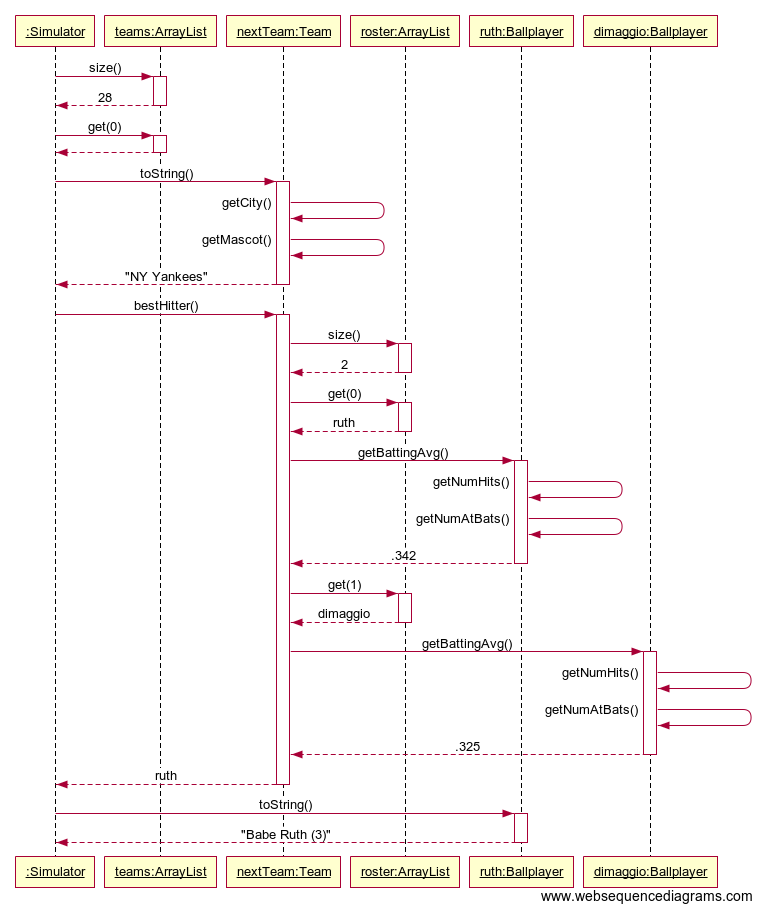
\includegraphics[width=1.1\textwidth]{baseballSeqDiag.pdf} % 1056x1180
\vspace{.1in}
\caption{A sequence diagram: Baseball example.}
\label{fig:baseballSeqDiag}
\end{figure}

\subsection{Sequence diagram features}

Now look at the enormous diagram in Figure~\ref{fig:baseballSeqDiag}. To get
your bearings, note these two important aspects of sequence diagrams:

\begin{compactitem}
\index{object}
\item The \textbf{\textit{objects}} (and occasionally classes) that
participate in this scenario \textbf{\textit{appear across the top}} of the
diagram. There is no inherent meaning to the order in which they appear, but
often objects that are involved earlier in the code path are on the left side.
\item The dashed line that extends down the page from each box ``goes with''
that object. Horizontal arrows that originate from (or point to) that line are
methods that object calls (or that are called on it).
\item \textit{\textbf{Time goes down.}} In other words, as the code path
executes in time, we move progressively further down the page.
\end{compactitem}

\subsection{What the arrows mean}

So we begin by looking at the upper-left corner, where the top-most arrow goes
from the ``\texttt{:Simulator}'' box to the ``\texttt{teams:ArrayList}'' box,
and is labeled ``\texttt{size()}''. As I'm sure you can guess, this corresponds
to the line of code: ``\texttt{int numTeams = teams.size();}'' which is the
first thing we do in \texttt{.printAllStars()}.

{\large \HandRight} \ Here's how you interpret \textit{any} arrow on a sequence diagram:

\begin{compactenum}
\index{method}
\item Every horizontal arrow is a method call. (Important: method calls are the
\textit{only} part of the code that can be shown on a sequence diagram.)
\item The vertical dashed line where the arrow \textit{starts} is the object
that makes that call. (In other words, if an arrow starts from a ``:Person''
box, then somewhere in a method of the \texttt{Person} class we can expect to
find this method being called.)
\item The vertical dashed line where the arrow \textit{ends} is the object on
which the method is \textit{being} called. (In other words, if an arrow ends
on a ``:Book'' box, then we're calling the method on that \texttt{Book}
object.)
\item The writing on the arrow is the name of the method being called, plus
any parameters.
\end{compactenum}

So, that first arrow in Figure~\ref{fig:baseballSeqDiag} means:
\vspace{-.1in}
\begin{center}
\begin{tabular}{m{.1in} m{4in}}
\large \HandRight & ``Somewhere in a method of the \texttt{Simulator} class, we're calling
\texttt{.size()} on an \texttt{ArrayList} object named \texttt{teams}.''
\end{tabular}
\end{center}

(Before you go on, read that sentence, and stare at that arrow, several times
and make sure you're absolutely certain of every detail. This one key idea is
the secret to understanding sequence diagrams.)

Notice that the arrow terminates on the top of a skinny box that extends a
centimeter or so down the \texttt{teams:ArrayList}'s vertical dashed line. This
skinny box represents \textit{the time during which the program is ``in'' the
\texttt{.size()} method.} It's not actually intended to specify a duration of
time (as in ``the \texttt{.size()} method will take 1.4 milliseconds to
complete'') but rather the-fact-that-it's-being-executed at all. In a moment,
we'll see that these skinny boxes can be (much) taller if we want our sequence
diagram to show detail about what happens \textit{inside} that method.

\subsection{Following the flow}

Okay. Let's continue down the diagram and see the rest of the action
unfolding. Keep your finger on Figure~\ref{fig:baseballSeqDiag} as we go so
you don't lose your place.

\begin{enumerate}
\itemsep.1em

\index{return@\texttt{return}}
\item The dashed vertical line pointing left with a ``28'' written on it is the
\textit{return value}. In this particular scenario, apparently there are 28
teams (\textit{i.e.}, 28 entries in the \texttt{ArrayList}).

\item The next call is to \texttt{.get()} the first entry in the list. Observe
how the line says literally ``\texttt{.get(0)}'' whereas the code has
``\texttt{.get(i)}'', with \texttt{i} being a loop variable. This is perfectly
fine. It means that as the code executes, the call to \texttt{ArrayList.get()}
is effectively passed the value \texttt{0} as an argument the first time it's
called, which is of course true. \textit{The fact that a loop is required is
implicit.} The designer, who created this sequence diagram, isn't spelling out
details like ``use a loop here'' for the programmer. Instead, she's
illustrating the intended pattern of method calls between objects -- the
programmer will infer the need for loops, local variables, \textit{etc.}

\item The dashed ``return value'' line is blank. That's okay too: it means the
designer didn't bother to specify a name for it. (Get used to design diagrams
containing differing levels of information in different places.)

\index{toString@\texttt{.toString()}}
\item Then \texttt{.toString()} is called on the returned \texttt{Team}
object. Why? Because we're \texttt{System.out.println()}'ing it, and as you'll
recall from p.~\pageref{pg:toString}, the \texttt{.toString()} method is
automatically invoked for any object that tries to be ``printed.'' So even
though our code doesn't explicitly say ``\texttt{.toString()}'' in it, the
method is nevertheless called, and is thus dutifully shown on the sequence
diagram.

\item Now pay close attention. Notice that the \texttt{.toString()} arrow
isn't followed by a dashed return value arrow right away. Instead, the skinny
box extends down the page an inch or more. This is because \textit{we're
showing what's happening inside \texttt{.toString()}}. In this case, there are
two bendy arrows going from the \texttt{nextTeam:Team} line \textit{back to
itself}. These mean that the methods \texttt{.getCity()} and
\texttt{.getMascot()} are being called by the \texttt{Team} object \textit{on
itself}. This may disorient you at first, but of course there's nothing really
strange about an object calling a method on itself. After all, our
\texttt{Team.toString()} method looks like this:

\begin{Verbatim}[fontsize=\footnotesize,samepage=true,frame=single]
public class Team {
    ...
    public String toString() {
        return this.getCity() + " " + this.getMascot();
    }
    ...
    private String getCity() { return this.city; }
    private String getMascot() { return this.mascot; }
}
\end{Verbatim}

Calling a method on ``\texttt{this}'' is exactly what's indicated by those
bendy arrows.

\item Now, finally, we get our dashed arrow back to ``\texttt{:Simulator}'',
with a return value of ``\texttt{NY Yankees}''. The control flow thus transfers
from \texttt{.toString()} back to \texttt{.printAllStars()}.

\index{bestHitter@\texttt{.bestHitter()}}
\item Next up is the \texttt{.bestHitter()} method, called later on in that
same \texttt{.println()} call. This commences an even longer skinny box,
because \texttt{.bestHitter()} has a lot to do. Here it is:

\begin{Verbatim}[fontsize=\scriptsize,samepage=true,frame=single]
    ...
    private Ballplayer bestHitter() {
        int numPlayers = roster.size();
        Ballplayer best = roster.get(0);
        for (int i=0; i<numPlayers; i++) {
            Ballplayer b = roster.get(i);
            if (b.getBattingAvg() > best.getBattingAvg()) {
                best = b;
            }
        }
        return best;
    }
}
\end{Verbatim}

You can see that after getting the size of the roster (in this case, only two
players since this is a long enough example as it is!) we get each
\texttt{Ballplayer} in turn, ask for his batting average, and compare it to
our ``best so far'' in a typical find-the-max-element type of loop.

\index{Ruth, Babe}
\index{Dimaggio, Joe}
All of this is faithfully represented in the sequence diagram. First, the
\texttt{Team} object calls \texttt{.size()} (and gets ``2'' back). Then it
calls \texttt{.get(0)} (and gets back a player; let's say Babe Ruth), and then
calls \texttt{.getBattingAvg()} on it (getting the number .342, a jaw-dropping
lifetime average, especially for a power hitter). A moment later, it does the
same with the second player (say, Joe Dimaggio) and gets his average (still
amazing, but ``only'' .325) for comparison.

\item More detail is shown inside the \path{Ballplayer.getBattingAvg()} calls.
That code looks like this:

\begin{Verbatim}[fontsize=\scriptsize,samepage=true,frame=single]
public class Ballplayer {
    ...
    public double getBattingAvg() {
        return ((double) this.getNumHits()) / this.getNumAtBats();
    }
    private String getNumHits() { return this.numHits; }
    private String getNumAtBats() { return this.numABs; }
    ...
}
\end{Verbatim}

and makes two ``self-calls'' to get this \texttt{Ballplayer}'s two relevant
statistics. Those calls are again shown as bendy loops.

\item Finally, the \texttt{Team} returns its best hitter (Babe Ruth in this
scenario) back to the \texttt{Simulator}, which again calls
\texttt{.toString()} implicitly, this time on the \texttt{Ballplayer} object.
That method returns the name of the ballplayer and his uniform number,
formatted nicely, for \texttt{Simulator.printAllStars()} to print.

\end{enumerate}

\subsection{Coming up for air}

That was a long journey through the weeds, because that sequence diagram
contained a boatload of stuff. In fact, one of the big takeaways here is that
\textit{a sequence diagram contains a ton of information about how to write
the code.}

A sequence diagram omits programming-specific details like whether to create
local variables and what to call them; whether you need a loop and what type
of loop you might choose; what the exact formula is for a computation, or the
logic to test for a condition; \textit{etc.} But it does present you with a
silver platter that says which objects of which types are intended to call
which methods on which other objects, and in what sequence.

In practice, I'd estimate that this works out to be about 70\% or so of the
decisions the programmer would otherwise have to make. What a windfall!

Before we move to our second example, let me tell you the two most common
errors I see among students trying to interpret (or create) sequence diagrams:

\vspace{-.1in}
\begin{enumerate}
\itemsep.5em
\item \textbf{Misinterpreting what the arrowhead-side of the arrow means.}
Each arrow points to a line which represents \textit{the object on which the
method is being called.} There's a great way to sanity check this: make sure
that the class (for whatever type of object the arrow is pointing to) actually
has a method of that name!

Figure~\ref{fig:rightWrongSeqDiag} shows some common mistakes. Neither of the
top two sequence diagram fragments can possibly be correct, because they show
an \texttt{.add()} method being called on a \texttt{Review} object. Now I ask
you: look at the class diagram -- do you see an \texttt{.add()} method on the
\texttt{Review} class? Nope. That means that right away, without even thinking
any further, you can rule out the top two sequence diagram attempts in that
figure.

\index{movie@\texttt{Movie}}
\index{review@\texttt{Review}}
The bottom two versions pass this test, because in those diagram
\texttt{.add()} is being called on a \textit{\texttt{Movie}} object, which
does indeed have an \texttt{.add()} method.

\begin{figure}
\centering
\includegraphics[width=0.9\textwidth]{rightWrongSeqDiag.pdf}  %
\caption{Many wrong ways to draw the sequence diagram arrow...and one right
way.}
\label{fig:rightWrongSeqDiag}
\end{figure}

\item \textbf{Misinterpreting what the non-arrowhead-side of the arrow means.}
Each arrow originates from a line which represents \textit{the object whose
code is making the method call} (on a different object, normally). 

To sanity check this, we can't look at the class diagram alone. We have to
think about what the code looks like. Suppose this were the case:

\begin{Verbatim}[fontsize=\small,samepage=true,frame=single]
class Editor {
    ...
    public void approve(Review r, Movie m) {
        ...
        m.add(r);
    }
}
\end{Verbatim}

Even before we saw this code snippet, we already knew that \texttt{.add()}
would be called on a \texttt{Movie} object (and passed a \texttt{Review}
object as an argument) because that's in line with the class diagram. But what
we learn now is \textit{where} that line of code exists. Is it written in a
method of the \texttt{Review} class? Or the \texttt{Movie} class? Nope -- it's
in the \texttt{.approve()} method \textit{of the \texttt{Editor} class.} That
tells us that the \textit{bottom} of the four sequence diagrams in
Figure~\ref{fig:rightWrongSeqDiag} is the correct one. The third one shows a
\textit{\texttt{Review}} making the method call, but if that were the case,
the ``\texttt{m.add(r)}'' line would be somewhere in \texttt{Review.java}.

\end{enumerate}

\section{Going forwards}

\vspace{-.1in}
{\large \textbf{Using a sequence diagram to guide the implementation}}

Now normally we won't be drawing a sequence diagram after we've written the
code, although that does actually happen sometimes, like when we want to
illustrate the behavior of a system to a new member of our programming team.
(It's usually easier for them to see the diagram at a glance than it is for
them to wade through a bunch of code and try to make sense of it.)

We'll now \textit{start} with a design (both class and sequence diagram), and
see what we can infer about what the code to implement it should look like.
Figures~\ref{fig:playlistClassDiag} and \ref{fig:playlistSeq} give the design,
which you are encouraged to study in detail.

\begin{figure}
\centering
\includegraphics[width=1.1\textwidth]{playlistClassDiag.pdf}
\caption{The playlist program's class diagram.}
\label{fig:playlistClassDiag}

\end{figure}
\begin{figure}
\centering
\hspace*{-.3in}
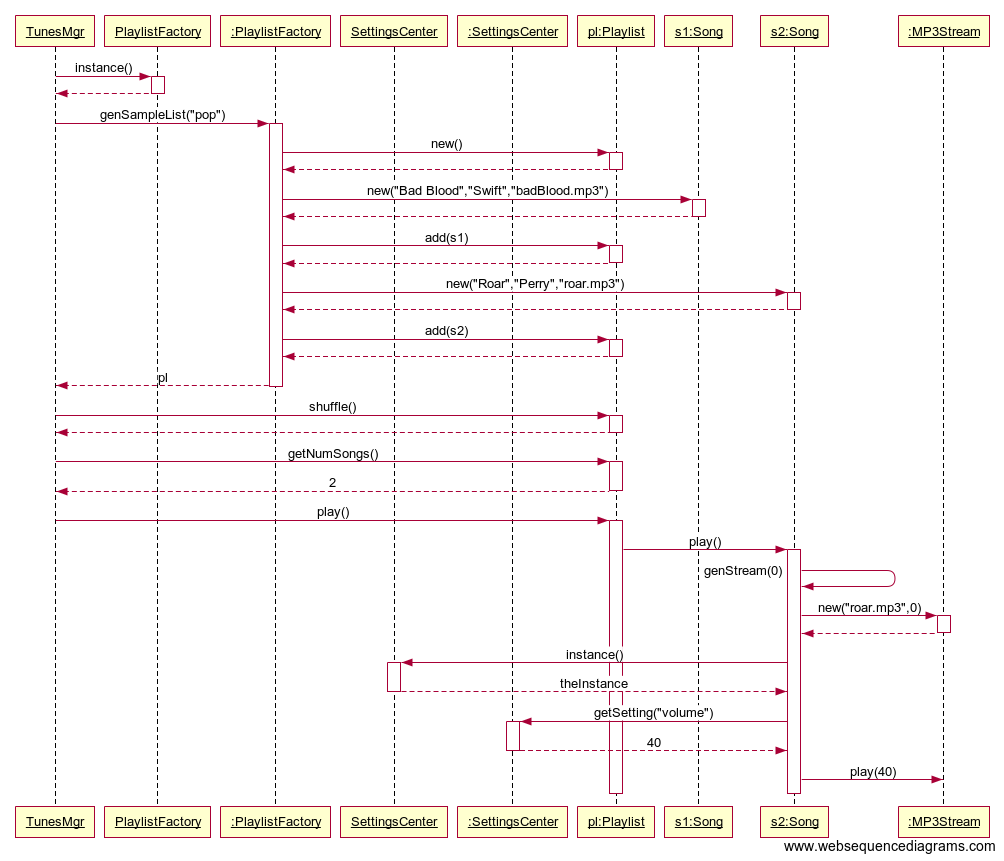
\includegraphics[width=1.1\textwidth]{playlistSeq.pdf}
\vspace{.1in}
\caption{One of the playlist program's sequence diagrams.}
\quad\quad\quad\quad\quad % hack to center caption
%\protect\phantom{.}}
\label{fig:playlistSeq}
\end{figure}

Here are some things we can read right off the sequence diagram (starting at
the top):

\begin{enumerate}
\itemsep.1em

\index{class@\texttt{class}}
\index{static@\texttt{static}}
\index{instance@\texttt{.instance()}}
\index{tunesMgr@\texttt{TunesMgr}}
\index{song@\texttt{Song}}
\index{playlistFactory@\texttt{PlaylistFactory}}
\index{genSampleList@\texttt{.genSampleList()}}
\item Something in the \texttt{TunesMgr} class will call \texttt{.instance()}
on the \texttt{PlaylistFactory} class. (Notice that the second box from the
left is missing a colon, so it must represent the \textit{class}
\texttt{PlaylistFactory} rather than an object of that type.) Since we're
calling \texttt{.instance()} on a class rather than an object, it had better
be \texttt{static}; and when we look at the class diagram, happily it is.

Furthermore, we can easily guess \textit{which} \texttt{TunesMgr} method is
making that method call, since there's only one listed for it:
\texttt{main()}. After calling \texttt{.instance()} on the class, it looks
like it calls \texttt{.genSampleList("pop")} on the object. Putting it all
together, we can surmise that this code should appear in our
\texttt{TunesMgr.java} file:

\begin{Verbatim}[fontsize=\footnotesize,samepage=true,frame=single]
class TunesMgr {
    public static void main(String args[]) {
        PlaylistFactory pf = PlaylistFactory.instance();
        Playlist p = pf.genSampleList("pop");
        ...to be continued...
    }
}
\end{Verbatim}

All we had to figure out for ourselves was to store the return values in
variables, which seemed like a good idea.

\item Switching scenes to the \texttt{PlaylistFactory}, we get a good sense of
the innards of its \texttt{.genSampleList()} method. The first couple of
arrows coming out of \texttt{:PlaylistFactory} say ``new'', which as you may
guess indicates an \textit{instantiation} and a constructor invocation. In
the first case, we're instantiating a new \texttt{Playlist} object. Apparently
the constructor for \texttt{Playlist} doesn't take any arguments (or the
sequence diagram author didn't bother specifying any). The \texttt{Song}
object we instantiate next, on the other hand, takes a slew of arguments: a
song title, artist, and filename.

After creating this new \texttt{Song}, we \texttt{.add()} it to the
\texttt{Playlist}. We then do the same for another \texttt{Song}. In sum,
here's the kind of thing that \texttt{.getSampleList()} must contain:

\begin{Verbatim}[fontsize=\scriptsize,samepage=true,frame=single]
class PlaylistFactory {
    ...
    Playlist genSampleList(String genre) {
        ...
        Playlist pl = new Playlist();
        Song s1 = new Song("Bad Blood", "Swift", "badBlood.mp3");
        pl.add(s1);
        Song s2 = new Song("Roar", "Perry", "roar.mp3");
        pl.add(s2);
		...
        return pl;
    }
    ...
}
\end{Verbatim}

Now lest we be too hasty, let's step back for a moment. The above code
might well not \textit{literally} be in \texttt{.getSampleList()}; after all,
it refers to specific, hardcoded songs. It also doesn't take into account the
value of \texttt{genre}; presumably, if we passed ``\texttt{rap}'' or
``\texttt{classical}'' as the argument, we'd get a different song selection. So
I'm not actually saying that you can read the code off the diagram without
thinking. What the sequence diagram tells us, though, is good information
about \textit{what kinds of things will happen} in each method. One could
imagine the real \texttt{.getSampleList()} reading song titles from a file or
from an Internet source depending on the genre, for instance. Even in that
case, though, all the sequence diagram essentials would be the same: we'd be
instantiating a new \texttt{Playlist} and \texttt{Song}s, adding the
\texttt{Song}s to the list, \textit{etc.}

\index{main method@\texttt{main()} method}
\item ``Back to \texttt{main()}!'' the sequence diagram announces. After
returning the \texttt{Playlist} (which Figure~\ref{fig:playlistSeq} suggests
we call ``\texttt{pl}'') our \texttt{main()} method commences calling three
methods on it. We can thus further flesh out our main method as follows:

\begin{Verbatim}[fontsize=\footnotesize,samepage=true,frame=single]
class TunesMgr {
    public static void main(String args[]) {
        PlaylistFactory pf = PlaylistFactory.instance();
        Playlist p = pf.genSampleList("pop");

        p.shuffle();
        int num = p.getNumSongs();
        p.play();
    }
}
\end{Verbatim}

Nothing explicitly told us to save the \texttt{.getNumSongs()} return value in
a variable, but we did it anyway. We're also not told what specifically we
would do with that information -- perhaps display it for the user, or estimate
the duration of the playlist based on it. At any rate, for now we'll just save
it and move on.

\index{play@\texttt{.play()}}
\item Finally, calling \texttt{.play()} on the \texttt{Playlist} turns around
and calls \texttt{.play()} on each of its \texttt{Song}s, not surprisingly. We
can thus deduce something like:

\begin{Verbatim}[fontsize=\footnotesize,samepage=true,frame=single]
public class Song {
    ...
    private ArrayList<Song> songs;
    ...
    public void play() {
        for (Song s: songs) {
            s.play();
        }         
    }
    ...
}
\end{Verbatim}

\index{mp3Stream@\texttt{MP3Stream}}
\index{settingsCenter@\texttt{SettingsCenter}}
\index{genStream@\texttt{.genStream()}}
\item As for \textit{\texttt{Song}'s} \texttt{.play()}
method\footnote{Interestingly, note that there are \textit{three} different
methods called \texttt{.play()} in this design, on each of three different
classes: \texttt{Playlist}, \texttt{Play}, and \texttt{MP3Stream}.}, it
apparently involves calling its own \texttt{.genStream()} method, which in
turn instantiates an \texttt{MP3Stream} object to do the actual playing. After
this, it gets the Singleton \texttt{.instance()} from the
\texttt{SettingsCenter} (note that arrows can go right-to-left on sequence
diagrams in addition to left-to-right) and gets the user's \texttt{"volume"}
setting. Finally, it calls \texttt{.play()} on its \texttt{MP3Stream} to play
at the correct volume. Putting it all together, we infer this sort of code:

\begin{Verbatim}[fontsize=\scriptsize,samepage=true,frame=single]
public class Song {
    ...
    public void play() {
        // ("0" means "start at the beginning of the song")
        MP3Stream s = this.genStream(0);  
        int vol = SettingsCenter.instance().getSetting("volume");
        s.play(vol);
    }
    ...
    public MP3Stream genStream(int pos) {
        ...
        return new MP3Stream(this.filename, pos);
    }
}
\end{Verbatim}

Here we choose to chain together the calls to \texttt{.instance()} and
\texttt{.getSetting()} rather than saving the \texttt{SettingsCenter} instance
to a variable. This is programmer's discretion. 



\end{enumerate}

Many challenges and questions still remain: how exactly do we go about
generating sample playlists based on genre? What algorithm will
\texttt{.shuffle()} use? Do we play all the songs in a row, back to back, or
do we insert a few seconds of silence in between? How exactly does the
\texttt{MP3Stream} read the bytes off the disk and send them to the audio
speakers? \textit{Etc.} These are important decisions, every bit as important
as what kind of wood and nails to use for each wall we frame. 

But the class diagrams and sequence diagrams have given us a tour of the whole
house as it was envisioned by the architect. We now have a framework into
which all the little decisions can be fit. And that's the first step towards
an elegant and maintainable program.



\chapter{Persistence and hydration}

Often, we want some of our objects to maintain their existence between
executions of the program. They're intended to be durable and lasting, and so
we need a way to record their details in some kind of permanent record so they
can be resurrected later.

Examples abound. Consider a social media app, where new users can register,
login, post messages, friend each other, \textit{etc.} We'd likely store
information about all this in various \texttt{User}, \texttt{Post},
\texttt{Profile}, and \texttt{FriendRequest} objects. But it sure would be a
bummer if all that data disappeared any time the server needed to be
restarted!

Or consider a drawing application, which we can use to create figures like
lines, rectangles, circles, and so forth, to create the kinds of diagrams
contained in this book. Our \texttt{Drawing}, \texttt{Line}, and
\texttt{Rectangle} objects, whose instances held information about position,
size, and color, would be next to useless if they weren't able to store
themselves permanently somehow, to be reloaded in a later execution of the
app. It would be like a word processor without a ``save'' function.

What we want is a way to \textbf{persist} (or save) an object, and
\textbf{hydrate} (or restore) it later. Persistence is taking an ephemeral,
in-memory object and writing it out to some form of permanent storage -- a
file in the filesystem, a database, a network drive, or anything else that
will stay put even when the program ends. Hydration is the reverse process:
resurrecting that stored version of the entity's state into a living,
breathing object once again.

\section{Java object serialization}

There are several ways to implement such operations. One, which I don't
recommend, is built into Java and is called ``serialization.'' The
\texttt{java.io} package has classes \texttt{ObjectOutputStream} and
\texttt{ObjectInputStream} for this purpose. The idea is that just as you can
write primitive types like integers and strings to a stream with familiar file
I/O operations, you can also read and write bona fide objects
themselves.\footnote{All objects that are saved and restored in this way must
be from classes that are declared to ``implement'' the
\texttt{java.io.Serializable} ``interface.'' We'll talk about implementing
interfaces in Section~\ref{sec:interfaces}.} Just open an
\texttt{ObjectOutputStream} to a file and call \texttt{.writeObject()}, and
the object you pass, in its entirety, will be saved in the file.
\texttt{ObjectInputStream.readObject()} performs the reverse process.

This all sounds like a great idea, but there's some serious practical
difficulties to consider. For one, \texttt{ObjectOutputStream} stores objects
in a \textbf{binary format} rather than a \textbf{text format}. This means
that the files it produces can't be easily analyzed -- they're compact, but
opaque, sequences of 1's and 0's. If you try to open such a file in a text
editor like \texttt{vim} to inspect what objects and values it contains,
you'll get gobbledy-gook. The upshot is that it's nearly impossible to debug
your program or even get visibility into what was saved.

Just as problematic is the fact that serialization is not
\textbf{forwards-compatible}. When you write an object to a stream in this
way, the data that is persisted is hard-wired to the particular version of the
class the object is a member of. This isn't a problem if your code is
completely, permanently stable. But during a development cycle, you're
constantly changing the nature of many classes, including their instance
variables, names, and types. As soon as you change a class in any significant
way, \textit{bam!!} all previously stored copies of objects are now
unreadable. When you try to hydrate them with \texttt{ObjectInputStream},
it'll break saying, ``whoa, the class of this stored object was an old version
of the class -- it doesn't match the current \texttt{.java} file.'' And that
data is, for all intents and purposes, lost.

I've learned the hard way that when you persist objects, you want to store
them in a format which is transparent and forwards-compatible. You need to be
able to inspect exactly what was stored, and have that data be readable even
if you change the class's definition later on.

\section{Using a relational (or non-relational) database}

An excellent solution for persistence and hydration is to use a Database
Management System (DBMS) like MySQL, PostgreSQL, or MongoDB. These products
specialize in this very task. Some, like those with ``SQL'' in the name,
create \textbf{relational databases} which hold rectangular tables of data
records, sort of like gigantic spreadsheets. Others are called
\textbf{non-relational} or \textbf{NoSQL databases} and can store data in a
more flexible, non-rectangular format. Programs in Java (or any other
language) can create \textbf{connections} to either kind of database, and
read/write to them with standard commands.

The reason I won't go further into this option is because it's really a
separate topic from OOA\&D, and merits a whole course in its own right (at
UMW, it's CPSC 350). Once you learn that material, it's really the best way to
do the whole persistence/hydration thing.

\section{Using plain text files}

In this book, I'll just explain how to do caveman-style persistence and
hydration: using plain text files. This will allow you to leverage your basic
file I/O knowledge from previous programming courses to achieve our purpose of
making objects persistent.

The first thing we need to decide is how to organize our storage. Should each
object have its own file? Should all objects of the same class be stored in
one file? Or should \textit{everything} we want to persist be stored in one
file?

There are arguments for all of these, and it really comes down to the needs of
the application. If we have a file-based save/restore paradigm, like our
drawing editor example from earlier, it probably makes sense to store
everything in a single file. When the user chooses ``save,'' we write their
entire drawing to the filename of their choice, and when they choose ``open,''
we read it back.

In a social network scenario, on the other hand, we probably want more
granularity. As soon as a user posts a new message or changes their status, we
want to create or re-write \textit{one} file (not our entire memory footprint)
with the updated information. This way we can write in little snippets as we
go, creating a bunch of files in a directory that collectively represent the
entire state of the application. When the system is taken down and rebooted
later on, it reads all those files to reconstruct its previous state.

\subsection{Example: a resort reservation system}

Here, let's assume that we want the first scenario: a single file that
contains all relevant information to the application. We'll create part of a
simple hotel reservation system, which stores and retrieves information about
various resort destinations. It consists of just two classes: \texttt{Resort},
objects of which represent individual hotels; and \texttt{ReservationSystem},
the main program.

For simplicity, I'm only going to show the parts of the program that are
related to persistence and hydration. (Clearly there are lots of other things
the code would need to do, like display lists of matching hotels in response
to searches, and actually make reservations.)

The key idea is this. Each class whose objects we want to save needs two
things:

\begin{compactitem}

\item For persistence, a \texttt{.persist()} method that writes the object out
to the \texttt{PrintWriter}\footnote{\texttt{PrintWriter} is a class in
\texttt{java.io} that has \texttt{.println()} methods for various data types.
I like it for that reason. Otherwise, it's essentially the same as any other
kind of \texttt{Writer}, like a \texttt{FileWriter}.} passed.

\item For hydration, a constructor that takes a \texttt{Scanner}\footnote{A
\texttt{Scanner} is a class in \texttt{java.util} that can parse primitive
types from a stream of text.} and creates a new object based on the
information queued up on that \texttt{Scanner}.

\end{compactitem}

Let's do the \texttt{Resort} class first. The key question is: what do we want
the persisted form of a \texttt{Resort} object to look like? Any way of
writing all the necessary information in a way that we can unambiguously get
it back will do. I vote for this:

\begin{Verbatim}[fontsize=\small,samepage=true,frame=lines]
Westword Spa and Surf
312-555-1234
5 stars
$$$
This luxurious beach property
is a pleasure for all who visit.
Dogs and cats welcome too!
.
\end{Verbatim}

The textual representation of a \texttt{Resort} consists of the following
parts:

\begin{compactenum}
\item A single line of text giving the resort's name.
\item A single line of text giving the resort's telephone number.
\item A single line of text with a digit from 1 to 5, followed by a space and
the String ``\texttt{stars}'' (or ``\texttt{star}'').
\item A single line of text with dollar signs, the number of which indicates
the expense of the resort (on a scale of \$ to \$\$\$\$).
\item One or more lines of text giving a description of the resort.
\item A line containing only a period. \label{item:delimiter}
\end{compactenum}

As you'll remember from your previous programming courses, that last item
(\#\ref{item:delimiter}) is called a \textbf{delimiter} since it ``delimits''
(marks the end of) the resort entry.

Now, for the Java class. Figure~\ref{fig:resort1} \textit{almost} has what we
want. Look at it carefully.

\begin{figure}[ht]
\centering
\begin{Verbatim}[fontsize=\footnotesize,samepage=true,frame=single]
class Resort {
    private String name, desc, phone;
    private int rating, cost;

    Resort(Scanner s) {
        name = s.nextLine();
        phone = s.nextLine();
        rating = s.nextInt();
        s.nextLine();    // read and discard the " stars" part.
        cost = s.nextLine().length();
        desc = "";
        String next = s.nextLine();
        while (!next.equals(".")) {
            desc = desc + next + "\n";
            next = s.nextLine();
        }
    }
    
    void persist(PrintWriter pw) {
        pw.println(name);
        pw.println(phone);
        pw.println(rating + " " + (rating == 1 ? "star" : "stars"));
        for (int i=0; i<cost; i++) {
            pw.print("$");
        }
        pw.println();  // newline for the $$$
        pw.println(desc);
        pw.println(".");
    }
}
\end{Verbatim}
\caption{Our first cut at the \texttt{Resort} class.}
\label{fig:resort1}
\end{figure}

\subsubsection{\texttt{Resort}: hydration}

The constructor is used for hydration. Perhaps the trickiest thing about it is
that we \textit{pass it a \texttt{Scanner} object}. Even if you've worked with
\texttt{Scanner} before, this may be a new idea to you: passing one around
between objects so that different objects can read different parts of a file.
But that's precisely what we're doing here. Remember that with file I/O, you
have a \textbf{cursor} open to a file, which is always ``at'' a particular
location within the file. Reading from the \texttt{Scanner} (perhaps using one
of the \texttt{.next*()} methods like \texttt{.nextInt()} or
\texttt{.nextLine()}) \textbf{advances} the cursor through the file to the
next bit.

So when a client calls ``\texttt{new Resort(someScanner)}'', they're saying
``this \texttt{Scanner}'s cursor is currently positioned right at the
beginning of some resort information. So please hydrate one \texttt{Resort}
object for me by reading just that much of the file.''

The constructor proceeds to do just that. It reads the name, phone number,
rating, cost, and description, in that order, ending when it reaches (and
reads past) the period (``\texttt{.}'') delimiter. I'll let you glance through
the code and see if you agree with my implementation here. There are a few
interesting nuances, like:

\begin{compactitem}

\item When reading the rating (``\texttt{4 stars}'') we call
\texttt{.nextInt()} to read the number part, and then \texttt{.nextLine()} to
read past and discard the rest of the line.

\item When reading the cost (``\texttt{\$\$\$\$}'') we take the length of the
string (the number of dollar signs) and store that number.

\item When reading the possibly-multi-line description, we continually keep a
lookout for the delimiter. As long as the lines we read are \textit{not} the
period on a line by itself, we append them to the end of our \texttt{desc}
inst var, along with the newline character (``\texttt{\textbackslash n}'') that
\texttt{.nextLine()} discards.

\end{compactitem}

All just fiddly stuff.

\subsubsection{\texttt{Resort}: persistence}

The inverse process of our constructor is our \texttt{.persist()} method,
which works similarly: given a \texttt{PrintWriter} -- to which other
information has quite possibly already been written -- write out the text
representation of this \texttt{Resort} object.

Just a few things of note here:

\begin{compactitem}

\item If you haven't seen the wacky syntax at the end of the
``\texttt{rating}'' line, it's worth knowing. It's called a ``conditional
expression'' or a ``question-mark-colon operator'' and is a compact way of
sticking a short \texttt{if}/\texttt{else} onto one line. It means ``if the
boolean expression before the question mark is true, replace this whole
expression with the thing before the colon; otherwise, replace it with the
thing after the colon.'' Less than legible to beginners, but a nice shortcut
for experts.

\item A simple \texttt{for} loop converts the integer \texttt{cost} into a
string of dollar signs. We also have an explicit \texttt{.println()} after
that loop so that we include the line feed after those dollar signs.

\item We explicitly write the delimiter (``\texttt{.}'') at the end of the
description, so that when read back by the hydration process, the constructor
knows where the description stops.

\end{compactitem}

Clearly the persistence and hydration code for a class need to be kept in
lock-step with each other. Adding a new field to the former, for instance,
necessitates us reading that field in the latter.

\subsubsection{Detecting the end of a sequence}

I said above that Figure~\ref{fig:resort1} is \textit{almost} what we want.
We're going to make one change to it. When a client calls ``\texttt{new
Resort(someScanner)}'', it's expecting the constructor to hydrate a
\texttt{Resort} object and hand it over. But consider: what if there are no
more \texttt{Resort} objects in the file?

Let's zoom out a second and appreciate the context in which the
\texttt{Resort} constructor will be called. We've made the design decision to
store all our application's information in a single file. This means that our
save file is going to have lots of resorts in it, back-to-back-to-back, each
separated from the following one by the period delimiter.

This in turn means that our code in \texttt{ReservationSystem} is going to be
calling ``\texttt{new Resort(someScanner)}'' \textit{in a loop} to hydrate all
the objects. This will work great until the point at which we hit the end of
the list. What then?

In that case, the \texttt{Resort} constructor can't be allowed to finish,
because \textit{it doesn't make sense for an object to be constructed at all}.
So what should the constructor do in that case? Throw an \texttt{Exception},
of course. This indicates to the client that the instantiation \textit{failed}
-- there is no \texttt{Resort} object to be constructed, and the client should
do what's appropriate in that event (in this case, simply stop reading from
the file).

The exception we throw can either be a ``plain old \texttt{Exception},'' or a
special type of exception that we create for this purpose. The latter approach
requires the technique of \textit{inheritance}, which we won't cover until the
next chapter. But I'll give you a preview. By simply creating a one-line
\texttt{NoMoreResortsException.java} file:

\begin{Verbatim}[fontsize=\small,samepage=true,frame=single]
class NoMoreResortsException extends Exception {}
\end{Verbatim}

voil\`{a}, we can now throw \texttt{NoMoreResortsException}s in addition to
plain old \texttt{Exception}s. This increases code readability (it's obvious
from the class name what this kind of exception indicates) and also allows us
to distinguish this type of exception from other kinds of things that might go
wrong (for instance, a bad filename or other problem accessing the
filesystem).

The only other question is: how does the constructor know when it's reached
the end of the sequence of resorts? Depending on how we choose to structure
the file, it might be when the end of the file is reached, or when some other
delimiter is encountered. Let's do the second case, and say that at the end of
the resorts list, our file will contain a line with these five characters:
``\texttt{-END-}''. When we hit this, we'll know there are no more resorts to be
hydrated.

Here's the modified \texttt{Resort} constructor:

\begin{Verbatim}[fontsize=\footnotesize,samepage=true,frame=single]
    Resort(Scanner s) throws NoMoreResortsException {
        name = s.nextLine();
        if (name.equals("-END-")) {
            throw new NoMoreResortsException();
        }
        phone = s.nextLine();
        rating = s.nextInt();
        s.nextLine();    // read and discard the " stars" part.
        cost = s.nextLine().length();
        desc = "";
        String next = s.nextLine();
        while (!next.equals(".")) {
            desc = desc + next + "\n";
            next = s.nextLine();
        }
    }
\end{Verbatim}

It's exactly the same except that after reading what it supposes is the
resort's name, the constructor sanity-checks that against the string
``\texttt{--END-}''. If they're equal, it realizes that it didn't read a
resort's name after all, but instead \textit{it hit the end of the list.} In
response, it abandons the rest of the constructor, \textit{refuses to
instantiate an object}, and throws the exception back to the caller.

\subsubsection{\texttt{ReservationSystem}: hydration}

And now, what does our overarching ``read and write the whole file'' code look
like? Again, it depends on the structure of the file itself. Let's say it's
formatted as in Figure~\ref{fig:wholeFile}. This file is comprised of the
following parts:

\begin{compactenum}
\item A line with the resort chain name.
\item The year this data is applicable to, followed by some other text
(``\texttt{ season}'').
\item Another line of preamble (the hyphens), which we just have to read
past.
\item A sequence of resort entries, each of which is delimited with a period.
\item The line ``\texttt{-END-}'' to indicate the end of the sequence.
\item A copyright notice, which we just have to read past.
\end{compactenum}


\begin{figure}[ht]
\centering
\begin{Verbatim}[fontsize=\scriptsize,samepage=true,frame=lines]
Holiday Inn resorts
2019 season
-------------------------
Westword Spa and Surf
312-555-1234
5 stars
$$$
This luxurious beach property is a pleasure
for all who visit. Dogs and cats welcome too!
.
Roadkill Motel
306-555-4444
1 star
$$
The 1970's-style armchairs aren't the problem:
the holes in the walls and the odorific properties
are. Traveler beware!
.
ABC Inn
123-456-7890
3 stars
$$  
Nothin' fancy, nothin' broken. Your basic motel 
for the budget (but hygiene-conscious) traveler.
.   
-END- 
Copyright (C) 2019
\end{Verbatim}
\caption{The file format for our resort reservation system.}
\label{fig:wholeFile}
\end{figure}

Given this structure, here's the way our \texttt{ReservationSystem}'s
constructor should work:

\begin{Verbatim}[fontsize=\footnotesize,samepage=true,frame=single]
public class ReservationSystem {
    private int year;
    private String chainName;
    private ArrayList<Resort> resorts;

    ReservationSystem(String filename) throws Exception {
        this.resorts = new ArrayList<Resort>();
        Scanner s = new Scanner(new FileReader(filename));
        this.chainName = s.nextLine();
        year = s.nextInt();
        s.nextLine();    // Read past " season"
        s.nextLine();    // Read past line of hyphens

        // Read all the resorts.
        try {
            while (true) {
                Resort r = new Resort(s);
                resorts.add(r);
            }
        } catch (NoResortException e) {
        }

        s.nextLine();    // Read past copyright
    }
}
\end{Verbatim}

Check out that \texttt{try}/\texttt{catch}/\texttt{while} loop construct
very carefully. It's short, but it's also a doozy. Inside the body of the
\texttt{try} block, we have what appears to be an \textit{infinite} loop:
after all, \texttt{while(true)} means ``forever.'' So we instantiate a
\texttt{Resort} object and add it to our \texttt{ArrayList}, do it again, do
it again, do it again...

But it's not really infinite and here's why: eventually, the \texttt{Resort}
constructor is going to discover that there aren't any more resort entries in
the file. When we ask it to hydrate the fourth \texttt{Resort} from
Figure~\ref{fig:wholeFile}, the constructor won't return: instead, it'll throw
a \texttt{NoMoreResortsException}. When that happens, we pop out of the
\texttt{try} block and into the \texttt{catch} block, \textit{which is outside
the body of the loop}. So we're officially done with the loop at that point,
and carry on to read the copyright information at the end and we're done.

And what does the \texttt{catch} block do? \textit{Nothing.} That may seem
pretty weird, but a moment's thought will convince you otherwise. What should
we do when we reach the end of the resorts? \textit{Simply carry on.} Even
though it's an \texttt{Exception}, it's not really an ``error.'' It just
means, ``oh, you wanted another \texttt{Resort} object, but actually there
aren't any. Carry on with your other business, Mr.~Client.''

To be crystal clear, here's what happens in the \texttt{try}/\texttt{while}
construct when we read Figure~\ref{fig:wholeFile}:

\begin{compactenum}
\item It hydrates a \texttt{Resort} object, and adds it to the
\texttt{resorts} \texttt{ArrayList}.
\item It hydrates a \texttt{Resort} object, and adds it to the
\texttt{resorts} \texttt{ArrayList}.
\item It hydrates a \texttt{Resort} object, and adds it to the
\texttt{resorts} \texttt{ArrayList}.
\item It tries to hydrate a \texttt{Resort} object...but catches the exception
instead, pops out of the \texttt{try} block (and therefore also the
\texttt{while} loop) entirely, and goes to the \texttt{catch} block.
\item The catch block does nothing.
\item It carries on reading the rest of the file.
\end{compactenum}

Note carefully that \textit{no exception is thrown from the
\texttt{ReservationSystem} constructor in this case!} Rather, the exceptions
thrown by the \textit{\texttt{Resort}} constructor are caught and dealt with
by the \texttt{ReservationSystem} constructor. The only time the
\texttt{ReservationSystem} constructor would throw an \texttt{Exception} is if
something went wrong when trying to read the file (in which case an
\texttt{Exception}, rather than a \texttt{NoMoreResortsException}, would be
generated).

\subsubsection{\texttt{ReservationSystem}: persistence}

Finally, the \texttt{.persist()} method of the \texttt{ReservationSystem}
class:

\begin{Verbatim}[fontsize=\small,samepage=true,frame=single]
    void persist(PrintWriter pw) {
        pw.println(chainName);
        pw.println("" + year + " season");
        pw.println("-----------------------------------");
        for (Resort r : resorts) {
            r.persist(pw);
        }
        pw.println("Copyright (C) " + year);
        pw.close();
    }
\end{Verbatim}

It's quite simple. The main part is simply calling the \texttt{.persist()}
method on each \texttt{Resort} object, so that they can persist themselves.
The stuff before and after is just for the boilerplate.



\chapter{Inheritance (1 of 2)}

\index{inheritance}
If one had to name object-oriented programming's most ``killer feature,'' a
good case could be made for \textbf{inheritance}. This specific technique for
code reuse and modular flexibility underlies much of the ``magic'' that happens
in well-architected OO programs, including most of the design patterns we'll
consider in later chapters. Developers need to know it, and know it well.

Interestingly, inheritance is used for two distinct (and essentially
unrelated) reasons to achieve two very different kinds of results. I call
these ``\textbf{top-down inheritance}'' and ``\textbf{bottom-up inheritance},
for reasons I'll explain; the more standard terms are \textbf{interface
inheritance} and \textbf{implementation inheritance}, respectively.

Curiously, when I was a young'un taking object-oriented programming in
college, we learned \textit{only} about the latter of these, and I was
mystified early in my career when I saw the former in action and had no idea
what the code was doing. Only then did I realize that although bottom-up
inheritance is indeed useful, top-down inheritance is the real game changer.
We'll cover both in this chapter.

\section{``Bottom-up'' (implementation) inheritance}

\index{inheritance!bottom-up (implementation)}
\index{object}
\index{class}
As you know, the Java API contains a class called \texttt{ArrayList}. The
class diagram below shows an abbreviated version of it. Already there's one
possibly unfamiliar element to you here: the literal word ``\texttt{Object}''.
It might seem odd to learn that there is a \textit{class} called
\textit{\texttt{Object}}, but that is indeed the case. And in fact this very
class will come back later in the chapter and play a major role in Java's
version of inheritance. For now, just consider that we are working with the
\textit{non}-generic \texttt{ArrayList} type -- \textit{i.e.} the user will
not declare ``\texttt{ArrayList<String>}'' but plain-ol' ``\texttt{ArrayList}''
-- so that the things that can be stored in it are ``\textit{any} type of
\texttt{Object}.'' That's why we're using the most general possible word here
as the argument of \texttt{.add()}, \texttt{.remove()}, \textit{etc.}

\begin{wrapfigure}{r}{5.5cm}
\vspace{-.2in}
\includegraphics[width=0.4\textwidth]{arrayList.pdf}
\caption{An abbreviated \texttt{ArrayList} class.}
\label{fig:abbrArrayList}
\end{wrapfigure}

\index{countUniqueArrayList@\texttt{CountUniqueArrayList}}
\index{client code}
Now suppose we were writing a program that needed to manage a bunch of
list-like data, and that \texttt{ArrayList} was just the ticket...except that
it was missing one or more important features. For example, maybe in addition
to inserting, removing, counting, \textit{etc.}, we also needed the ability to
\textit{count the number of unique elements} in a list. The client code we'd
like to be able to write is in Figure~\ref{fig:dreamCountUnique}.

\begin{figure}[hb]
\centering
\begin{Verbatim}[fontsize=\footnotesize,samepage=true,frame=single]
public static void main(String args[]) {
   ArrayList n = new ArrayList();
   n.add("Harry");
   n.add("Ron");
   n.add("Hermione");
   n.add("Harry");
   n.add("Harry");
   n.add("Dumbledore");
 
   System.out.println(n.get(3));         // prints "Harry"
   System.out.println(n.size());         // prints 6
   System.out.println(n.countUnique());  // *should print 4 (but no such method)
}
\end{Verbatim}
\caption{Some client code we'd \textit{like} to be able to write in our
hypothetical program.}
\label{fig:dreamCountUnique}
\end{figure}

This client code already works except for the last line, which of course
contains a method we just made up. It's sad that \texttt{ArrayList} meets all
our needs except this one teensy one.

\index{hasa association@``has-a'' association}
\index{association!has-a@``has-a''}
Several ways to get around this limitation come to mind. We could use a
\textbf{has-a} association between \texttt{ArrayList} and a new class of our
devising, ``\texttt{CountUniqueArrayList}.'' Each \texttt{CountUniqueArrayList}
would have an \texttt{ArrayList} ``under the hood'' which it would use to
actually store the data. Figure~\ref{fig:countUnique1} gives the idea.

\begin{figure}
\centering
\includegraphics[width=0.9\textwidth]{countUnique1.pdf}  % 700x190
\caption{A first approach to enhancing a regular \texttt{ArrayList}.....}
\label{fig:countUnique1}
\end{figure}

\index{method!pass-through}
We could code our \texttt{.countUnique()} in a variety of ways, and now the
last line of Figure~\ref{fig:dreamCountUnique} would work like a charm.
Trouble is...the other lines wouldn't work anymore. Obviously we have to be
able to do ``normal'' \texttt{ArrayList} things with our class as well as
calling our new special method. So we'd have to duplicate all the other
\texttt{ArrayList} methods on our new class, and have them ``pass through'' the
arguments to the underlying \texttt{ArrayList} that it holds. The result is
the unwieldy, repetitive monstrosity in Figure~\ref{fig:countUnique2}, which
is obviously not a good solution. Here's what each of our ``pass-through''
methods would look like:

\begin{Verbatim}[fontsize=\small,samepage=true,frame=single]
public class CountUniqueArrayList {
    private ArrayList al;

    public void add(Object o) {
        al.add(o);
    }
    public int size() {
        return al.size();
    }
    ...etc...
}\end{Verbatim}


\begin{figure}
\centering
\includegraphics[width=0.9\textwidth]{countUnique2.pdf}  % 700x190
\caption{.....but this necessitates duplicating all the original methods.}
\label{fig:countUnique2}
\end{figure}

At the very least, this is clumsy, duplicative, and error-prone. But it could
be even worse, if the \texttt{ArrayList} class evolves. Suppose the Java API
expands to include a \texttt{.shuffle()} method on \texttt{ArrayList}, which
randomly jumbles the contents of the list? Every \texttt{ArrayList} in every
line of Java code in the world could instantly take advantage of that. But our
stunted \texttt{CountUniqueArrayList} could not: it would have to be changed
to add a \texttt{.shuffle()} pass-through method before it could do what any
other \texttt{ArrayList} could automatically do.

\label{page:inheritanceArrows}
\begin{figure}[h]
\centering
\includegraphics[width=0.7\textwidth]{inheritanceArrows.pdf}
\caption{Diagrammatic elements for inheritance. (Compare with
Figure~\ref{fig:assocArrows}.)}
\label{fig:inheritanceArrows}
\end{figure}

\index{isa association@``is-a'' association}
\index{association!is-a@``is-a''}
The solution is to use inheritance. \textit{Instead of ``\textbf{has-a},'' an
inheritance association means ``\textbf{is-a}.''} (See
Figure~\ref{fig:inheritanceArrows}.) Instead of each
\texttt{CountUniqueArrayList} \textit{having} an \texttt{ArrayList} under the
hood, we're declaring that a \texttt{CountUniqueArrayList} in fact
\textbf{\textit{is}} an \texttt{ArrayList}. This gives it all the rights and
privileges of any \texttt{ArrayList} including all of its methods and instance
variables. All the code in Figure~\ref{fig:dreamCountUnique} \textit{instantly
just flat works}. The UML equivalent is shown in
Figure~\ref{fig:countUnique3}. Note carefully that we use an open-triangle
arrowhead to designate inheritance, and that there are no other navigability,
multiplicity, or role indicators.

\begin{figure}[h]
\centering
\includegraphics[width=1\textwidth]{countUnique3.pdf}
\caption{Bottom-up inheritance in action. (Note the open-triangle arrowhead.)}
\label{fig:countUnique3}
\end{figure}

\index{superclass}
This may seem like cheating. Surely if we want to call a method on an object,
we're entitled to see that method in the UML diagram for that object's class?
Clearly, \texttt{.add()}, \texttt{.get()}, and \texttt{.size()} do not appear
in \texttt{CountUniqueArrayList}'s box. But the magic of inheritance makes it
work anyway. The rule is that you can call a method on an object if that
method is defined on the object's class...or on any \textbf{superclass}.
\texttt{ArrayList} is said to be the ``superclass'' of
\texttt{CountUniqueArrayList}. And that brings us to a slew of equivalent
terminology.

\index{subclass}
\begin{samepage}
All of these expressions mean exactly the same thing:
\begin{center}
\small
A is-a B\\
A inherits from B\\
A specializes B\\
A is a subclass of B\\
A is a subtype of B\\
A is a derived class of B\\
B generalizes A\\
B is the superclass of A\\
B is the supertype of A\\
B is the base class of A\\
\end{center}
\end{samepage}

You know something's an important concept when there are a zillion equivalent
terms for it. And so it is with inheritance.

Sometimes we say ``A is a class, and B is its superclass.'' Other times we say
``B is a class, and A is a subclass.'' These aren't contradictory statements --
it's like saying I'm both a son (of my mom and dad) and also a father (of my
three kids). You can totally be a son and a father at the same time. And a
class can be both a superclass and a subclass.

\index{inheritance hierarchy}
By the way, if you have sharp eyes, you'll have noticed I said ``or
\textit{any} superclass'' a few paragraphs ago. That's because if A inherits
from B, B can in turn inherit from some other class, which can itself inherit,
\textit{etc.} All the classes and their related sub/superclasses form what's
known as an \textbf{inheritance hierarchy}.

\subsection{Under the hood}

You might wonder how this magic works behind the scenes. It's actually pretty
simple. When we instantiate a \texttt{CountUniqueArrayList}, we not only
allocate memory for all the \texttt{CountUniqueArrayList}-specific parts (if
any), but also for its superclass parts.

\index{student@\texttt{Student}}
\index{person@\texttt{Person}}
Let's take a different example so that we know what the ``parts'' actually
are.\footnote{It may or may not surprise you that I honestly don't know what
instance variables the \texttt{java.util.ArrayList} class has, or what they're
named. This is a perfect example of the wonders of encapsulation: millions of
people across the globe use \texttt{ArrayList}s every day, and do not know or
care how they function internally!} Figure~\ref{fig:studentClass} shows two
classes in an inheritance relationship: a \texttt{Student} \textbf{is-a}
\texttt{Person}. While a \texttt{Person} in general has a \texttt{name} and 
and \texttt{age}, the special type of person called a ``\texttt{Student}'' also
has an \texttt{eagleOneID} and a \texttt{gpa}.

\begin{figure}
\centering
\includegraphics[width=0.9\textwidth]{studentClass.pdf}
\caption{A \texttt{Student} is a special kind of \texttt{Person}, but a
genuine \texttt{Person} nonetheless.}
\label{fig:studentClass}
\end{figure}

\begin{samepage}
Now when we instantiate each of these classes:

\begin{Verbatim}[fontsize=\footnotesize,samepage=true,frame=single]
    public static void main(String args[]) {
        Person tony = new Person();
        tony.setName("Tony Stark");
        tony.setAge(39);

        Student peter = new Student();
        peter.setName("Peter Parker");
        peter.setAge(17);
        peter.setGPA(3.85);
        peter.setEagleOneID("000518989");
    }
\end{Verbatim}
\end{samepage}

the objects of each type look like Figure~\ref{fig:studentObject}. See how the
\texttt{Student} object has \textit{both} the required \texttt{Student} and
\texttt{Person} instance variables, since it is both a \texttt{Student} and a
\texttt{Person}. To Java, the fact that the \texttt{Person} ``stuff'' is in a
separate little chamber inside the \texttt{Student} box is just a detail.

\begin{figure}
\centering
\includegraphics[width=0.9\textwidth]{studentObject.pdf}
\caption{A \texttt{Student}, and an ordinary \texttt{Person}, in the heap.}
\label{fig:studentObject}
\end{figure}

\section{``Bottom-up'' (implementation) inheritance}
The reason I call this technique ``bottom-up inheritance'' is that in order to
use the special features of your new class, \textit{you need to know you have
an instance of the subclass.} In the code above, we couldn't call
\texttt{.setGPA()} on an ordinary \texttt{Person}: it would have to be a
\texttt{Student}. We couldn't call \texttt{.countUnique()} on just any Joe
\texttt{ArrayList} -- only \texttt{CountUniqueArrayList}s have that special
method. Hence, the code that uses the classes views the hierarchy ``from the
bottom-up''; \textit{i.e.}, from the perspective of the subclass. In fact, if
all we instantiate are \texttt{Student}s (not \texttt{Person}s), then our
\texttt{main()} method doesn't even need to know there \textit{is} a
superclass. To \texttt{main()}, it's all about \texttt{Student}s, and the fact
that you can do ordinary person-ish things to a \texttt{Student} -- like set
its \texttt{age}, or ask it to \texttt{.work()} or \texttt{.sleep()} -- seem
just like other aspects of \texttt{Student}s.

The conventional term for this, ``implementation inheritance,'' comes from the
fact that the reason we're inheriting is \textit{to steal the implementation.}
Someone has already gone to the trouble of writing an \texttt{ArrayList} class
-- or a \texttt{Person} class -- and we don't want to reinvent the wheel. So
we make use of that implementation (the code in the methods) and just add
whatever else we want to the mix.


\section{``Top-down'' (interface) inheritance}

\index{inheritance!top-down (interface)}
Now top-down inheritance is where the real action is.

\index{sortedArrayList@\texttt{SortedArrayList}}
Let's go back to our \texttt{ArrayList} example, and this time I'm going to
write a different subclass, called ``\texttt{SortedArrayList}.''
Figure~\ref{fig:sortedAL} shows this arrangement. The open-triangle arrow and
the word ``is-a'' are just the same. The one thing that might strike you as
odd, though, is that the methods on the subclass are \textit{also all on the
superclass}. Hey, we already had an \texttt{.add()}, an \texttt{.insert()},
and a \texttt{.set()}: what good is our new class that just duplicates this?
As it turns out, a \textit{lot}.

\begin{figure}
\centering
\includegraphics[width=0.9\textwidth]{sortedAL.pdf}
\caption{Top-down inheritance in action.}
\label{fig:sortedAL}
\end{figure}

To explain why, first let me articulate my motive for creating the
\texttt{SortedArrayList} type in the first place. I might have a program that
needs to store various bits of data in \texttt{ArrayList}s -- a common enough
task -- but it needs some of those lists to \textit{always remain in sorted
order}. Exactly what ``in order'' means depends on the data type, but we could
expect for \texttt{Integer}s it would be numerical order, for \texttt{String}s
alphabetical order, \textit{etc.}

It's easy to imagine a program that would need this feature. Perhaps it needs
to print the various lists in some kind of reliable sequence, or to perform
fast lookup via a binary search. Anyway, the point is: if I create a
\texttt{SortedArrayList}, I'm doing so because I want a guarantee that no
matter what I do to that list, I can always get the stuff out quickly, and
sorted.

Now if you think it through, you'll realize this is a different kind of
situation than we had with \texttt{CountUniqueArrayList}. Previously, we had a
\textit{new feature} we wanted to add to an existing class -- an
\texttt{ArrayList} could do many things, but not count its number of distinct
elements, and so we tacked that feature on to the top of it. But now, we don't
want a new feature so much as \textit{different behavior for the original
features.} We don't want to add any new methods, but have \textit{the existing
methods act differently.} And thus is the essence of top-down inheritance.

\index{override}
\index{method!overriden}
Before we see it in action, let's think about the implementation. You'll
notice that in Figure~\ref{fig:sortedAL} only \textit{some} of the methods
appear in the subclass. These are called \textbf{overridden} methods: we say
that \texttt{SortedArrayList}'s \texttt{.add()} ``overrides'' the base class's
\texttt{.add()}. Now can you figure out why those particular three methods are
the ones we chose to override?

If you're sharp, you'll realize that those three methods are the only ones
which, if we called the ordinary \texttt{ArrayList} version, would threaten to
jeopardize the sorted nature of the list:

\begin{itemize}
\itemsep.1em

\item If we have a sorted list, and \texttt{.add()} an item to it, our new
expanded list might be unsorted if \texttt{.add()} just tacks the new item on
to the end. Hence, \underline{\textbf{we must override \texttt{.add()}}} with
a version that adds the new element \textit{in the correct place}.

\item If I have a sorted list, and \texttt{.remove()} an element from it, the
shorter list will still be sorted. So the superclass's \texttt{.remove()}
doesn't mess anything up, and we can stick with it. No need to add a version
to \texttt{SortedArrayList} at all.

\item Whether the list's elements are sorted or not, \texttt{.size()} acts the
same for Pete's sake, so we hardly need to override that one.

\item On the other hand, if we \texttt{.insert()} an element at a specific
location, we'll mostly likely disturb the ordered-ness, so
\underline{\textbf{we must override \texttt{.insert()}}} as well, so that it
puts the new element only where it truly belongs.

\item The \texttt{.get()} method is an easy call: retrieving element \#9 out
of a list doesn't have any different behavior if the elements are sorted or
not, so we leave that one out.

\item Lastly, though, \underline{\textbf{we must override \texttt{.set()}}}
since changing one element's value could throw the ordered-ness out of kilter,
requiring resorting.

\end{itemize}

If you followed all that, you'll realize that the choice of which methods to
override in the subclass wasn't an arbitrary one. It was dictated directly by
the behavior we wanted our subclass to guarantee and preserve. Methods whose
default implementations (in the superclass) wouldn't work for our new type (in
this case, those that threatened to jeopardize the order) must be replaced
with versions appropriate to the subclass.

The word ``override'' is a good one, and it conveys almost exactly what it
means, although don't make the mistake of thinking that the ordinary
\texttt{ArrayList}'s \texttt{.add()} method is completely obliterated by what
we've done. \textit{Au contraire}, for plain-Jane \texttt{ArrayList}s all over
the world, that original \texttt{.add()} code will still run. Only if the
object in question is one of our special subtype -- only if it's a
\texttt{SortedArrayList} in addition to being a plan \texttt{ArrayList} --
will our new method be substituted. Put another way, we're not ``overriding
the \texttt{.add()} method for \textit{everybody},'' just for objects of our
new special type.

\subsection{Test your intuition}

\begin{samepage}
Okay, now to drill the concept all the way home. I want to ask you a question.
Before reading on, consider the code below and ask yourself ``what will its
output be?'' (Commit to an answer before you continue.)

\index{Thor}
\index{Banner, Bruce}
\index{Captain America}
\index{Hulk}
\index{getMad@\texttt{.getMad()}}
\begin{Verbatim}[fontsize=\small,samepage=true,frame=single]
    public static void main(String args[]) {
        SortedArrayList sal = new SortedArrayList();
        sal.add("Thor");
        sal.add("Bruce Banner");
        sal.add("Captain America");
    
        getMad(sal);
    
        for (int i=0; i<sal.size(); i++) {
            System.out.println("Hero #" + i + " is " + sal.get(i));
        }
    }

    private static void getMad(ArrayList al) {
        al.set(0,"Hulk");
    }
\end{Verbatim}
\end{samepage}

To figure this out, we first observe that the code is instantiating our
\textit{new} special kind of \texttt{ArrayList}: a \texttt{SortedArrayList}.
Therefore, we know that when \texttt{sal.add()} is called, \textit{it's our
new \texttt{.add()}} that will get executed. (Later in \texttt{main()}, we
call \texttt{sal.size()}, and this will of course trigger the ordinary
\texttt{.size()} since we didn't override that method.)

Now the big question, and the point of this exercise, is to consider what
happens \textit{inside} the \texttt{getMad()} function. Note very carefully
that \texttt{getMad()} takes an argument of type \textit{\texttt{ArrayList}},
not \texttt{SortedArrayList}. So \texttt{getMad()}, you might say, is itself
unaware that \texttt{SortedArrayList}s even exist, let alone that it's about
to be given one.

So I ask you: will \texttt{ArrayList}'s ordinary \texttt{.set()} method be
called, or will it be \texttt{SortedArrayList}'s new,
ensure-the-list-stays-sorted \texttt{.set()} that will take over?

The critical answer is: \textit{the subclass's method will be called, even
though the function itself doesn't know it's dealing with a subclass.}
\texttt{SortedArrayList.set()} will be called in this case, which will swap
\texttt{Hulk} with \texttt{Captain America} to keep the list alphabetically
sorted, giving this output:

\begin{Verbatim}[fontsize=\small,samepage=true,frame=single]
    Hero #0 is Captain America
    Hero #1 is Hulk
    Hero #2 is Thor
\end{Verbatim}

This surprises lots and lots of folks. It certainly surprised me when I
learned it (considerably after graduating college). I originally reasoned as
follows: ``\texttt{getMad()} was written to take an ordinary
\texttt{ArrayList}, and hence its code was designed with only
\texttt{ArrayList}s in mind. Surely this means that our three-hero-list, when
\texttt{getMad()} receives it, will be treated just as any normal
\texttt{ArrayList} would be. All that special overriding method stuff only
happens when we \textit{know} we're dealing with a \texttt{SortedArrayList} in
particular.''

The exact opposite is true. And it turns out that's how we want it to be.
Consider this very example: what good is a \texttt{SortedArrayList} if it
doesn't stay sorted? That was the whole point of the subclass! Yet we'd be
threatening to violate this very principle if we ever passed it into contexts
which didn't know it needed to be sorted, and hence unwittingly jumbled it up.
We must guarantee that \textit{every time} \texttt{.add()},
\texttt{.insert()}, or \texttt{.set()} is called on it, our new functionality
is triggered, whether or not the user of the object even knew that.


\subsection{``Masquerading'' and ``smuggling''}

\index{inheritance!top-down (interface)}
Now why do I call this ``top-down inheritance?'' The reason is that unlike with
bottom-up inheritance, you can use objects of your new subclass
\textit{without knowing they're of that subclass, or that there even is a
subclass.} As a user of the classes -- like \texttt{main()}, above -- you're
looking at the inheritance hierarchy from the top down.

\index{masquerading}
\index{smuggling}
A couple of other descriptive words I like to use for this are ``masquerading''
and ``smuggling.'' In the above example, the \texttt{SortedArrayList}
\texttt{sal} is masquerading as an \texttt{ArrayList} -- pretending to be one
for the sake of the \texttt{getMad()} function. (And of course it's not
actually ``pretending'' because a \texttt{SortedArrayList} truly
\mbox{\textbf{is-a}} \texttt{ArrayList}.) From \texttt{main()}'s point of
view, we smuggled a \texttt{SortedArrayList} into the \texttt{getMad()}
function, in cognito. Little did \texttt{getMad()} know that it wasn't even
dealing with an ordinary object of the base class. It was fooled by the
disguise.

\pagebreak
\subsection{Why this matters}

\index{decoupling}
The reason this idea is so powerful is that it allows programmers to decouple
the \textit{what} from the \textit{how}.

A chunk of code that only knows about the superclass (like \texttt{ArrayList})
can dictate \textit{what} to do with it. ``First I'll \texttt{.add()} these
three elements, then I'll \texttt{.remove()} one, then get the
\texttt{.size()}, \textit{etc.}''

In response to these method calls, the object itself -- perhaps of a
specialized subclass -- decides \textit{how} to carry out each one. An
ordinary \texttt{ArrayList} tacks the new element onto the end when it's told
to \texttt{.add()} one, whereas a \texttt{SortedArrayList} decides to stick it
in the appropriate place to preserve the order. The original code chunk can be
blissfully ignorant of how the details of \texttt{.add()}, \texttt{.insert()},
\textit{etc.}~work for any particular type of \texttt{ArrayList}.

\index{Super Smash Bros}
\index{Zelda}
\index{Peach}
If you're a videogamer, think of it in Smash Bros.~terms. Every character in
the game looks different, has different attack stats, different animations for
punching and falling, a different ``up smash'' and ``side special,'' and so
forth. But the main game engine code that coordinates the interaction between
characters on a stage doesn't have to worry about all those details. It can
simply say, ``hey, character \#1, your player just input a dash-left. Display
the appropriate animation please.'' The object for character \#1, who may
happen to be Zelda, then displays her determinedly zooming to the left with
her hair flowing behind her.

The game then says, ``hey, character \#4, you just got punched. First, tell me
your weight class so I know how far the knockback should be.'' If character \#4
is Peach, her object responds, ``I'm in the medium weight class.'' The game
then says, ``thanks. Now display your `hit stun' animation from your current
position up to coordinates 562, 431.'' The Peach object then shows her
character flying through the air with her umbrella in a tizzy.

\index{separation of concerns}
For even moderately complex programs, this ability to compartmentalize these
two jobs is crucial -- otherwise you end up with a 500-line function that's a
mass of spaghetti code. Software engineers call this decoupling
``\textbf{separation of concerns},'' and it is among the most important
principles in all of software development.
\vspace{1in}
\pagebreak

\section{``Cool! Can we do both?''}

A common question at this point is whether top-down and bottom-up inheritance
can be combined in a single class. The answer is yes! If you create a
subclass \texttt{A} of another class \texttt{B}, you could have some methods
of \texttt{A} override the existing methods of \texttt{B}, and you could also
have some brand new methods in \texttt{A} that weren't present in \texttt{B}.

Any code that deals with \texttt{B} objects will automatically work for
\texttt{A} objects also, and your new method implementations will be called
when it does. And you can write code that calls your brand new methods, as
long as that code \textit{knows it's dealing with a \texttt{A}}.

It's not super common to combine the techniques, but I've seen it done.

\section{A word of warning}

I'll finish this chapter with an observation from my years coding. Inheritance
tends to be both an \textit{underused} feature and an \textit{overused}
feature.

What I mean is that programmers (even experienced ones, sadly) sometimes fail
to recognize situations in which inheritance would be appropriate, and their
code becomes less elegant and more brittle as a result. Even more worrying,
I've seen more than one ``inheritance-happy'' programmer in my career use it
where it's \textit{not} called for. And this turns out to be even worse.

Although there are shades of grey, the basic rule for knowing when inheritance
is appropriate can actually be boiled down to a single principle:

\index{isa association@``is-a'' association}
\index{association!is-a@``is-a''}
\begin{quote}
\textbf{Remember that ``is-a'' means ``is-a.''}
\end{quote}

\index{subclass}
The time \textit{not} to use inheritance is when you see some code that you
want to reuse, but you really \textit{don't} have a conceptual ``subtype'' in
mind.

\index{runner@\texttt{Runner}}
\index{performance@\texttt{Performance}}
\index{race@\texttt{Race}}
An actual example: suppose your team is building a database system for 5k and
10k race results. There's a \texttt{Runner} class with inst vars like
\texttt{name} and \texttt{gender} and \texttt{dateOfBirth}. Then you say,
``all right: to record a performance in a particular race, we need all that
information about the runner, \textit{plus} the bib number, finish time, date
and location of the race.''

You may be tempted (as a colleague of mine once was) to create a
\texttt{Performance} class which \textit{inherits} from \texttt{Runner}. After
all, every \texttt{Performance} object would then possess all the necessary
attributes -- those of the racer, and those of the race. What's not to like?

Well, there are two problems. One is conceptual: could one possibly claim that
a \texttt{Performance} \textbf{is-a} \texttt{Runner}?! Obviously not. The very
fact that you could call \texttt{.getGender()} on a \texttt{Performance}
object, or pass a \texttt{Performance} to a \texttt{Race.register()}
method defies logic.

The other problem is practical: as these two nonsensically-joined classes
evolve, more pressure builds in the system that exposes the design flaw. When
a data entry mistake is corrected, for example, changing a \texttt{Runner}'s
name from \texttt{"Stanly"} to \texttt{"Stanley"}, only one of Stanley's
performances will have its \texttt{name} corrected; the other independent
copies for his other performances remain out of date. Even worse, suppose the
need arises for different (legitimate) subtypes of \texttt{Runner}:
\texttt{AmateurRunner} and \texttt{CompetitiveRunner}, say. Now
the \texttt{Performance} class is really in a bind: it only inherits from the
more general type, and would have to proliferate itself awkwardly
(``\texttt{AmateurPerformance}'' and ``\texttt{CompetitivePerformance}'') just
to stay in sync.

The lesson here is that your object-oriented model should strive to faithfully
reflect conceptual reality; it should not use design features in gimmicky ways
to achieve short-term programming wins. Always ask yourself ``does this choice
of classes really make \textit{sense}?'' as your guiding question.



\chapter{Inheritance (2 of 2)}
\label{ch:inheritance2}

\index{inheritance}
I split what was once a long inheritance chapter into two. So you're probably
back from a snack break, a nap, or a game of Ultimate. Let's get warmed up
again.

\index{zoo}
A class diagram for a ``Zoo'' program is in Figure~\ref{fig:zooClass}. Study
the code on the following page (Figure~\ref{fig:zooCode}) and predict its
output.

\begin{figure}[ht]
\label{zooExample}
\centering
\includegraphics[width=0.9\textwidth]{zooClass.pdf}
\caption{A class diagram for the Zoo program.}
\label{fig:zooClass}
\end{figure}

\index{animal@\texttt{Animal}}
\index{cow@\texttt{Cow}}
\index{duck@\texttt{Duck}}
\index{bear@\texttt{Bear}}
\index{bird@\texttt{Bird}}
\index{move@\texttt{.move()}}
\index{makeNoise@\texttt{.makeNoise()}}
We have an \texttt{Animal} class with a number of subclasses, and one of them
even has its \textit{own} subclass. In each case, we override one, both, or
neither of the base class's methods.

\begin{figure}
\begin{Verbatim}[fontsize=\scriptsize,samepage=true,frame=single]
class Animal {                           class Bird extends Animal {
  public void makeNoise() {                public void makeNoise() {
    System.out.println("Growl!");            System.out.println("Chirp");
  }                                        }
  public void move(int dist) {             public void move(int dist) {
    for (int i=0; i<dist; i++) {             System.out.println("Flap");
      System.out.print("tramp ");          }
    }                                    }
    System.out.println();                
  }
}                                        class Duck extends Bird {
                                           public void makeNoise() {
                                             System.out.println("Quack");
class Cow extends Animal {                 }
  public void makeNoise() {              }
    System.out.println("Mooooo");        
  }
}                                        class Bear extends Animal { }


class Zoo {
  public static void main(String args[]) {
    ArrayList<Animal> zoo = new ArrayList<Animal>();
    zoo.add(new Animal());
    zoo.add(new Bird());
    zoo.add(new Cow());
    zoo.add(new Bear());
    zoo.add(new Duck());
    generateCacophony(zoo);
  }

  private static void generateCacophony(ArrayList<Animal> animals) {
    for (Animal a: animals) {
      a.makeNoise();
      a.move(3);
      System.out.println();
    }
  }
}\end{Verbatim}
\caption{The Zoo program.}
\label{fig:zooCode}
\end{figure}

\begin{samepage}
The output of the program, as you can easily verify, is:

\begin{Verbatim}[fontsize=\footnotesize,samepage=true,frame=single]
Growl!
tramp tramp tramp 

Chirp
Flap

Mooooo
tramp tramp tramp 

Growl!
tramp tramp tramp 

Quack
Flap
\end{Verbatim}
\end{samepage}

\index{inheritance!top-down (interface)}
Lots of top-down inheritance here. Notice that the \texttt{Bear} class is
completely unchanged from its superclass: evidently, the generic animal
behavior works fine for bears, at least as far as moving and making noise
goes. This is not an error.

You also may have noticed that the \texttt{Bird}'s \texttt{.move()} method
completely ignores its \texttt{distance} argument. That, too, is not a
problem.

\index{tree}
\index{inheritance hierarchy}
Finally, and most importantly, note that the \texttt{Duck} class does not
override \texttt{.move()}, but its superclass (\texttt{Bird}) does, and so a
\texttt{Duck} will ``\texttt{Flap}'' like ordinary \texttt{Bird}s
do. The rule is: when a method is called on an object, the code in its class
is called, unless the class doesn't define that method. In that case, Java
looks for the method in its immediate superclass, then its superclass's
superclass, \textit{etc.}~all the way up the inheritance hierarchy, calling
the first one it finds. This makes sense: since a \texttt{Duck} \textbf{is-a}
\texttt{Bird}, it is sensible to make it move like a \texttt{Bird} rather than
like a generic \texttt{Animal}.

\section{Polymorphism}

\index{polymorphism}
This technique goes by a funny name, by the way: \textbf{polymorphism}. It's
one of those geeky-sounding words useful for slinging at parties when you want
an annoying person to move away from you.

\index{transparent}
I define polymorphism (specifically, ``subtype polymorphism,'' which is what
we're dealing with here) as \textit{transparently treating objects differently
based on their type.} The word ``transparently'' means ``without the
programmer having to worry about it.''

Essentially, polymorphism is another way to think about top-down inheritance.
We have a generic set of operations (like ``move'' and ``make noise''), each
of which can be personalized in custom ways by specific subclasses, but which
clients can simply call at the desired times without having to be aware of
those subclasses. ``The right thing'' simply happens based on the object's
type, without the programmer having to resort to a giant chain of if/else
statements or some other monstrosity. This is because the language itself
automatically dispatches the method call to the correct code.

In terms of the concrete zoo example, polymorphism basically says: ``the way
you direct any animal to make noise is the same: telling a duck to make noise
uses the exact same code as telling a cow to make noise. Yet different things
happen in each case, because of how Java enables the subtype-customization to
take place."

\subsection{\texttt{instanceof} is evil}

\index{instanceof operator (evil)@\texttt{instanceof} operator (evil)}
It may help you understand this if I contrast it with a \textit{non}-example
of polymorphism.

\index{Pok\'{e}mon}
\index{hyperbeam}
\index{thunder shock}
\index{attack@\texttt{.attack()}}
Suppose we have a \texttt{Pokemon} class, instances of which represent various
fictional fighting critters and their moves and stats. We also have a
\texttt{Power} class used to represent a particular superpower like ``thunder
shock'' or ``hyperbeam.'' Each special type of power will be its own subclass
of \texttt{Power}, in true object-oriented inheritance style. And for this
simple example, we'll say that each \texttt{Pokemon} has just one ``primary
power'' that it can use in combat. Whenever a \texttt{Pokemon} object's
\texttt{.attack()} method is called, it will use its primary power on the foe
it is passed.

\index{modularity}
Figure~\ref{fig:wrongPokemon} shows the \textbf{WRONG} way to code this. The
\texttt{.attack()} method itself, in the \texttt{Pokemon} class, is
scrutinizing its \texttt{primaryPower} object, figuring out what subclass it
is and responding appropriately. You can see the (evil) Java
\texttt{instanceof} operator in use here. It is a way of determining at
run-time whether or not an object is of a particular class. \textbf{Using
\texttt{instanceof} is almost always bad programming practice} since it
violates encapsulation, reduces modularity, and eschews polymorphism.
Among other things, this design creates a gigantic (and ever-growing, as more
powers are added to the program) \texttt{if}/\texttt{else} chain to do the
work that Java already does automatically. And that huge type-checking
mechanism, besides being unwieldy and error-prone, is plopped right inside the
\texttt{Pokemon} class, which is not the right place for it. (That code
concerns various types of \textit{powers}, not \textit{Pok\'{e}mon}.)

\begin{figure}[ht]
\begin{Verbatim}[fontsize=\small,samepage=true,frame=single]
public class Pokemon {

    private Power primaryPower;

    public void attack(Pokemon foe) {
        if (primaryPower instanceof Thundershock) {
            // do the "thundershock" stuff to the foe
        }
        else if (primaryPower instanceof RoarOfTime) {
            // do the "roar of time" stuff to the foe
        }       
        else if ...
    }
}

public class Power {
    ...
}

public class Thundershock extends Power {
    ...
}

public class RoarOfTime extends Power {
    ...
}
\end{Verbatim}
\caption{The {\color{red} \underline{\textbf{WRONG}}} way to implement
Pok\'{e}mon powers, using the \texttt{instanceof} operator.}
\label{fig:wrongPokemon}
\end{figure}

\index{roar of time}
\index{useAgainst@\texttt{.useAgainst()}}
Figure~\ref{fig:rightPokemon}, on the other hand, shows a good, healthy,
proper OO design for the Pok\'{e}mon model. None of that
\texttt{if}/\texttt{else} junk is even necessary, and the \texttt{Pokemon}'s
\texttt{.attack()} method becomes a one-liner, as it should be. Java will
automatically call the proper ``thunder shock'' code, ``roar of time'' code,
``hyperbeam'' code, or whatever, without us having to try to do its work for
it. And adding a new \texttt{Power} is just a matter of creating a new,
encapsulated subclass, with its own \texttt{.useAgainst()} code. Neither the
\texttt{Power} superclass nor the \texttt{Pokemon} class need be disturbed by
this addition. It all works seamlessly.

\definecolor{darkgreen}{rgb}{0,.65,0}
\begin{figure}[ht]
\begin{Verbatim}[fontsize=\small,samepage=true,frame=single]
public class Pokemon {

    private Power primaryPower;

    public void attack(Pokemon foe) {
        this.primaryPower.useAgainst(foe);
    }
}

public class Power {
    public void useAgainst(Pokemon foe) {
        // use the basic, default power on the foe
    }
}

public class Thundershock extends Power {
    public void useAgainst(Pokemon foe) {
        // do the "thundershock" stuff to the foe
    }
}

public class RoarOfTime extends Power {
    public void useAgainst(Pokemon foe) {
        // do the "roar of time" stuff to the foe
    }
}
\end{Verbatim}
\caption{The {\color{darkgreen} \underline{\textbf{right}}} way to implement
Pok\'{e}mon powers, using subtype polymorphism.}
\label{fig:rightPokemon}
\end{figure}
\section{Getting abstract}

\subsection{Abstract methods}

\index{zoo}
\index{animal@\texttt{Animal}}
\index{cow@\texttt{Cow}}
\index{duck@\texttt{Duck}}
\index{bear@\texttt{Bear}}
\index{bird@\texttt{Bird}}
\index{move@\texttt{.move()}}
\index{makeNoise@\texttt{.makeNoise()}}
Okay, back to the Zoo example from p.~\pageref{zooExample}. For each type of
animal, it was up to the subclass to decide whether to override a method or
not. If the subclass was happy with the base class's behavior (like
\texttt{Cow} was with \texttt{.move()}, or \texttt{Bear} was with everything)
it could just ignore that method and default to ordinary animal behavior.

\index{getNumChromosomes@\texttt{.getNumChromosomes()}}
\index{chromosome}
What if we had a method, though, where there was no reasonable default
behavior to define? Let's add a method \texttt{.getNumChromosomes()} which
will return the number of DNA molecules in that species. Unlike making noise,
which we might plausibly say is ``growling, unless further specified for a
particular animal,'' perhaps there isn't any ``default number of chromosomes''
that makes sense.\footnote{Consider: a fruit fly has only 8 chromosomes, while
a tasmanian devil has 14, a human has 46, a potato 48, a silkworm 56, and a
catfish 104. Given these examples, what default value would have any merit?}

Note that we still want to be able to call \texttt{.getNumChromosomes()} on
\textit{any} \texttt{Animal}, no matter what type. So it's no good to just
leave the method out of the \texttt{Animal} class and only define it on
subclasses.

\index{abstract method}
The solution to our dilemma is to make \texttt{.getNumChromosomes()} an
\textbf{abstract method}. ``Abstract'' means that even though it's defined in a
superclass -- with a name, parameter list, and return type -- there's not
actually any \textit{code} for it there! Here's what it looks like:

\begin{Verbatim}[fontsize=\small,samepage=true,frame=single]
class Animal {     // (not finished yet...)
    abstract public int getNumChromosomes();
    ...
}
\end{Verbatim}

It looks a little strange, with a semicolon prematurely truncating the method
signature. But by doing this, we're declaring that even though there's no
method \textit{body} for \texttt{.getNumChromosomes()} in the \texttt{Animal}
class, we still want to be able to call it on an \texttt{Animal}. Individual 
subclasses provide their own implementation; for example:

\begin{Verbatim}[fontsize=\small,samepage=true,frame=single]
class Cow extends Animal {
    public int getNumChromosomes() {
        return 60;
    }
    ...
}
\end{Verbatim}

Notice that the subclasses do \textit{not} include the keyword \texttt{abstract}
on the method.

\vspace{.7in}
\subsection{Abstract classes}

Now I know what you're thinking. ``This is all fine, but what if we have a
plain-old-\texttt{Animal} object and call \texttt{.getNumChromosomes()} on
it?'' 

\begin{Verbatim}[fontsize=\small,samepage=true,frame=single]
    Cow c = new Cow();
    int numc = c.getNumChromosomes();   <-- returns 60
    Animal a = new Animal();
    int numa = a.getNumChromosomes();   <-- ???
\end{Verbatim}

There's no code to run for a generic \texttt{Animal}, so what value would we
get back?

\index{instantiation}
This is indeed a dilemma, and Java solves it in the only sensible way: it says
\textit{you can't make a plain-old-\texttt{Animal} anymore.} The rule is: if
any method of a class is abstract, \textbf{the class itself must be abstract},
which means it is \textit{un-instantiatable.} In other words, the Java
compiler forces us to amend our \texttt{Animal} class as follows:

\begin{Verbatim}[fontsize=\small,samepage=true,frame=single]
abstract class Animal {                         
    public void makeNoise() {            
        System.out.println("Growl!");      
    }                                    

    public void move(int distance) {     
        for (int i=0; i<distance; i++) {   
          System.out.print("tramp ");      
        }                                  
        System.out.println();              
    }

    abstract public int getNumChromosomes();
}                                      
\end{Verbatim}

If we ever try to write the code ``\texttt{new Animal()}'', Java will (rightly)
stop us with a compilation error.

\begin{Verbatim}[fontsize=\footnotesize,samepage=true]
Animal.java:5: error: Animal is abstract; cannot be instantiated
        new Animal();
        ^
1 error
\end{Verbatim}

\begin{samepage} Note that every instantiatable subclass needs to be
non-\texttt{abstract}, and therefore \textit{it must have a body for every one
of its methods}, defined in either itself or in one of its superclasses. For
example, as soon as we add the \texttt{abstract}
\texttt{.getNumChromosomes()}, our \texttt{Cow.java} suddenly won't compile
either:

\begin{Verbatim}[fontsize=\footnotesize,samepage=true]
Cow.java:4: error: Cow is not abstract and does not override abstract
method getNumChromosomes() in Animal
    class Cow extends Animal {}
    ^
1 error
\end{Verbatim}
\normalsize
\end{samepage}

So we'll need to define \texttt{.getNumChromosomes()} in \texttt{Cow} and
\texttt{Bear} (or else make them \texttt{abstract}). What about \texttt{Duck}
and \texttt{Bird}? It depends on which of these classes (if either) we want to
be \texttt{abstract}. If we want to be able to ``\texttt{new Bird()}'' and also
``\texttt{new Duck()}'', then at \textit{least} \texttt{Bird} will have to
provide a \texttt{.getNumChromosomes()} method. (And \texttt{Duck}'s would be
optional. If in fact \texttt{Duck}s have a different number of chromosomes
than ordinary \texttt{Bird}s, we'd want to also make one on the \texttt{Duck}
class.) If, on the other hand, we're happy for \texttt{Bird} to be abstract
(and thus un-instantiatable), we could choose to define it \textit{only} on
\texttt{Duck} and call it a day. It all depends on what makes sense for the
domain.

Putting all this abstract stuff together, here are the rules:

\begin{enumerate}
\itemsep.1em
\item A class cannot be instantiated if it's declared \texttt{abstract}. (Only
its subclasses possibly can be.)
\item If there is any \texttt{abstract} method on a class, the class itself
must be declared \texttt{abstract}.
\item If a class \texttt{A} inherits from some other class \texttt{B}, and
\texttt{B} has abstract method(s) on it, \texttt{A} must provide
implementation(s) for all of those methods, or else \texttt{A} be declared 
\texttt{abstract} as well.
\end{enumerate}

\subsection{UML notation}

\index{abstract method}
\index{abstract class}
\index{stereotype}
There are two different ways to mark a method or class as \texttt{abstract} in
UML. One is to put the name of the method or class in italics. That works well
if you're using a design tool like ArgoUML or Rationale Rose to create your
diagrams. Otherwise, if you're doing it by hand, you add a
(``$\ll$abstract$\gg$'') stereotype. I've shown both approaches in
Figure~\ref{fig:zooClassAbstract}.

\begin{figure}
\centering
\includegraphics[width=0.9\textwidth]{zooClassAbstract.pdf}
\caption{Using \textit{italics}, and the $\ll$abstract$\gg$ stereotype, to
indicate abstract classes and methods.}
\label{fig:zooClassAbstract}
\end{figure}

\section{That's just super}

\index{super@\texttt{super}}
\subsubsection{Calling a superclass's methods with ``\texttt{super.}''}

Occasionally, it will make sense for a method in a class to explicitly call a
method in its superclass. For instance, suppose we said, ``When asked to make
noise, a \texttt{Duck} should `\texttt{Quack}' but then \textit{also} do
whatever ordinary \texttt{Bird}s usually do.'' We would write that as follows:

\begin{Verbatim}[fontsize=\footnotesize,samepage=true,frame=single]
class Duck extends Bird {
    public void makeNoise() {
        System.out.println("Quack");
        super.makeNoise();
    }
}
\end{Verbatim}

The ``\texttt{super.}'' prefix (pronounced ``super dot'') says to call the
version of \texttt{.makeNoise()} that's defined in the \texttt{Bird}
class, not the \texttt{Duck} one. (And a good thing, too: otherwise we'd have
an infinite loop with \texttt{.makeNoise()} repeatedly calling itself!)
Written this way, a \texttt{Duck} will make this noise:

\vspace{-.15in}
\begin{Verbatim}[fontsize=\small,samepage=true,frame=none]
  Quack
  Chirp
\end{Verbatim}
\vspace{-.15in}

\index{chipmunk@\texttt{Chipmunk}}
As another example, we might define a class \texttt{Chipmunk} that moves twice
as rapidly as normal animals. If we defined its \texttt{.move()} method thus:

\begin{Verbatim}[fontsize=\footnotesize,samepage=true,frame=single]
class Chipmunk extends Animal {
    public void move(int distance) {
        int doubleDist = distance * 2;
        super.move(doubleDist);
    }
}
\end{Verbatim}

then calling \texttt{.move(3)} on a \texttt{Chipmunk} object would print this:

\begin{Verbatim}[fontsize=\small,samepage=true,frame=none]
  tramp tramp tramp tramp tramp tramp
\end{Verbatim}

\index{encapsulation}

By the way, students often have a question here, and maybe you do too. They ask
whether they can call \texttt{super.super.move()} to invoke the ``grandparent's
method.'' The answer is \textbf{no}, for reasons having to do with
encapsulation. It's fine for a \texttt{Duck} to know it's a subclass of
\texttt{Bird}, but it shouldn't know what \texttt{Bird}'s superclass is, nor
even that \texttt{Bird} \textit{has} a superclass. That knowledge (which we
would be baking in to our program through a ``\texttt{super.super.}''\ call) is
outside the realm of the \texttt{Duck} class, and therefore should not be known
to it. If later, for instance, we refactor our code and make \texttt{Bird} its
own class instead of inheriting from \texttt{Animal}, \texttt{Duck} would break
if it had a ``\texttt{super.super.}''.

\subsubsection{Invoking a superclass's constructor with ``\texttt{super}'' (no
dot)}

\index{constructor}
\index{initialization}
You've known ever since p.~\pageref{page:instantiateConstructor} that whenever
an object is instantiated, one of that class's constructors is called. This is
indeed the case, but here's a new wrinkle: when an object is instantiated,
\textit{a constructor in its superclass is also called.} This is because in
order to ``set up'' the \texttt{Duck} stuff (initialize its inst vars,
\textit{etc.}), we also need to set up its \texttt{Bird} stuff, and for that
matter its \texttt{Animal} stuff. Since a \texttt{Duck} \textbf{is-a}
\texttt{Bird}, which in turn \textbf{is-a} \texttt{Animal}, it's imperative
that we have a valid \texttt{Animal} object before trying to make it a
special kind of \texttt{Animal} (and similarly, a valid \texttt{Bird} before
we make a special kind of \texttt{Bird}).

\index{student@\texttt{Student}}
\index{prof@\texttt{Prof}}
\index{person@\texttt{Person}}
This usually happens automatically, but can need some special coaxing if
you're passing arguments to constructors. An example is the code snippet in
Figure~\ref{fig:inhConstrCode} (whose class diagram is in
Figure~\ref{fig:inhConstrClass}). Here, the only constructor for the
\texttt{Person} class is one that takes a \texttt{String} argument; hence, we
must pass it a \texttt{String} if we want to instantiate one. In the
\texttt{Student} constructor (which takes a couple arguments of its own) we
call ``\texttt{super(name)}'' which passes the \texttt{name} the subclass was
given and passes it up to its superclass's constructor. In the
\texttt{Prof} constructor, we take a \texttt{"Dr.\ "} on to the front of
the name before passing it the superclass. Note that there's no ``dot'' after
these \texttt{super()}s; that's how we indicate we want to call the
constructor, rather than an ordinary method.

Somewhat weirdly, in Java the call to \texttt{super()} must be the
\textit{first} line of the constructor. That's because Java says, ``a
\texttt{Student} is a special type of \texttt{Person}. So if you want to be a
\texttt{Student}, you have to first be a fully-baked \texttt{Person}. Only
then will we get around to the \texttt{Student}-specific stuff.'' (Note this
restriction does \textit{not} apply to ``\texttt{super.}'' (``super dot'')
method calls; they can be put anywhere.)

\begin{figure}[ht]
\begin{Verbatim}[fontsize=\scriptsize,samepage=true,frame=single]
class Person {                    
    private String name;          
    protected Person(String n) {           class Prof extends Person {
        this.name = n;                         private String dept;
    }                                          Prof(String n, String d) {
}                                                  super("Dr. " + n);
                                                   this.dept = d;
class Student extends Person {                 }
    private double gpa;                    }
    private int year;
    Student(String name, int year) {
        super(name);
        this.gpa = 0.0;
        this.year = 1;  // Freshman
    }
}
\end{Verbatim}
\caption{The interaction between constructors when inheriting.}
\label{fig:inhConstrCode}
\end{figure}

\index{protected@\texttt{protected}}
\index{subclass}
\index{abstract class}
One other thing on this \texttt{Person}/\texttt{Prof}/\texttt{Student}
example: we have defined the \texttt{Person} constructor to have
\textbf{\texttt{protected}} visibility. As you may recall from
Figure~\ref{fig:visibilityLevels} on p.~\pageref{fig:visibilityLevels},
\texttt{protected} visibility (denoted in UML with a hashtag) means that it
can only be called by a class in the same package \textit{or a subclass}. It's
useful in situations like this that involve inheritance: by making the
\texttt{Person} constructor \texttt{protected}, we're saying that no one
outside the package can instantiate a plain-old \texttt{Person}: instead they
must instantiate a subtype, which can then call the constructor from below.
This is related, but not quite the same, as declaring a method
\texttt{abstract}. (The difference being that \texttt{abstract} classes can't
be instantiated \textit{anywhere}, even in the same package.)

\begin{figure}
\centering
\includegraphics[width=0.9\textwidth]{inhConstrClass.pdf}
\caption{The class diagram for Figure~\ref{fig:inhConstrCode}.}
\label{fig:inhConstrClass}
\end{figure}


\section{Pure abstraction: Java interfaces}
\label{sec:interfaces}

\index{interface@\texttt{interface}}
We've now seen several examples of superclasses. Sometimes they have all
concrete (opposite of abstract) methods, and a subclass can pick and choose
which ones it wants to override. Sometimes, they have one or more
\texttt{abstract} methods, which the subclass \textit{must} override, or else
be un-instantiatable.

What if we push that idea all the way in the abstract direction: a ``pure''
abstract class, with only abstract methods? Is that any use?

\index{implements@\texttt{implements}}
Yes, and probably more than you realize right now. I'll get to the reasons
this is so powerful in a page or two, but for now let's just learn the syntax.
In Java, instead of a pure abstract class, you can create something called an
\textbf{interface}, which is essentially the same thing but which gives
considerable more flexibility. An interface is a template of sorts, with
\textit{no instance variables} and \textit{no method bodies}. Classes that
\textbf{implement} an interface promise to create a method body for each of
the methods in the interface.

\index{class@\texttt{class}}
In UML (see Figure~\ref{fig:interface}), an interface looks almost exactly
like a class. The only differences are: (1) there are
(sometimes\footnote{Designers aren't consistent about this, I've found. Some
do include all three compartments for an interface, even though the middle one
must by definition be empty.}) only two compartments instead of three, and (2)
the \textbf{stereotype} $\ll$interface$\gg$ appears in the name box (recall
``stereotypes'' from p.~\pageref{stereotype}).

\begin{figure}[ht]
\centering
\includegraphics[width=0.9\textwidth]{interface.pdf}
\caption{Two classes that implement interfaces.}
\label{fig:interface}
\end{figure}

\index{triangle ($\triangle$)}
\index{line!dashed (-\ -\ -)}
We indicate ``implements an interface'' with a \textit{dashed} line that
otherwise looks exactly like an inheritance arrow (recall
Figure~\ref{fig:inheritanceArrows} from p.~\pageref{page:inheritanceArrows}).

\index{storable@\texttt{Storable}}
\index{connection}
In Figure~\ref{fig:interface}, both of the classes in our racers 
application need to store and load objects from the database. Hence, both of
them implement the \texttt{Storable} interface, which defines two methods, one
for storing and one for loading. The code for that much would look like:

\begin{Verbatim}[fontsize=\scriptsize,samepage=true,frame=single]
interface Storable {
    void store(DBConn c);
    void load(DBConn c);
}

class Race implements Storable {       class Runner implements Storable {                        
    private Date date;                     private String name;
    private String loc;                    private String gender;
    private int maxRunners;                public void store(DBConn c) {
    public void store(DBConn c) {         ...
        ...                                }
    }                                      public void load(DBConn c) {
    public void load(DBConn c) {          ...
        ...                                }
    }                                  }                                          
}                                       
\end{Verbatim}

\index{runner@\texttt{Runner}}
\index{participant@\texttt{Participant}}
\index{register@\texttt{.register()}}
Some Java syntax idiosyncrasies: an \texttt{interface} has only method
signatures (return type, method name, parameter lists) followed by a
semicolon, just as with abstract methods. However, the methods are
\textit{not} marked as \texttt{abstract}, nor \texttt{public} nor anything
else. Note also that we don't say the class ``\texttt{extends}'' the interface,
but rather ``\texttt{implements}'' it.

In the same figure, we have \texttt{Runner} also implementing another
interface: \texttt{Participant}. Presumably there are also other types of
participants (volunteers, walkers, wheelchair racers, walkers, rock bands that
play on the sidewalks) that can \texttt{.register()} for races, and if they
want to be able to participate, their classes must implement this one-method
interface. We augment the code as follows:

\begin{Verbatim}[fontsize=\scriptsize,samepage=true,frame=single]
interface Participant {
    int registerFor(Race r);
}

class Runner implements Storable, Participant {                        
    private String name;
    private String gender;
    public void store(DBConn c) {
         ...
    }
    public void load(DBConn c) {
         ...
    }
    int registerFor(Race r) {
        ...
    }
}                                            
\end{Verbatim}

Take note of the fact that the \texttt{Runner} class definition has
\textit{two} \texttt{interface} names in its declaration line, separated by a
comma. 

And that takes us, at last, to the reason Java \texttt{interface}s matter:
\textbf{\textit{because a class can implement more than one of them.}}

\index{inheritance!multiple}
\index{C++}
You might be thinking, ``okay, but couldn't we just have inherited from more
than one abstract class, and accomplished the same thing without this new
`interface' notion?'' The answer is \textbf{no}: Java does not allow
\textbf{multiple inheritance}, which is when a class has more than one
superclass. The reasons are somewhat lengthy to explain, and will be omitted
here, but suffice to say that languages that choose to support multiple
inheritance (C++ is among them) have some knotty problems to solve. For
instance, what if class \texttt{A} inherits from both \texttt{B} and
\texttt{C}, and both \texttt{B} and \texttt{C} have their own
\texttt{.doThis()} method. What code, then, would this line trigger?

\begin{Verbatim}[fontsize=\small,samepage=true]
        A a = new A();
        a.doThis();       <-- ? Whose "doThis()"?
\end{Verbatim}

How can it choose between \texttt{B}'s and \texttt{C}'s perfectly acceptable
implementations of \texttt{.doThis()}? Or should it run both of them, and if
so in what order?

\index{Gosling, James}
\index{inheritance!bottom-up (implementation)}
\index{inheritance!top-down (interface)}
James Gosling and the other designers of Java took a look at this problem and
decided that multiple inheritance wasn't worth the hassle. I happen to think
they were right, and for one simple reason: although programmers often want to
use multiple \textit{top-down} inheritance, they rarely want to use multiple
\textit{bottom-up} inheritance. And it's the latter that gives rise to all the
paradoxes and strange corner cases. As long as a class simply wants to
masquerade as one of several different things (as opposed to wanting to steal
method implementations and inst vars from more than one superclass), ``multiple
inheritance'' turns out not to be a big deal. One of Java's big wins was
allowing multiple interfaces to be implemented, not multiple classes to be
inherited from, thereby sidestepping the whole issue.

\begin{samepage}
So the bottom line is that in Java, a class can \textit{inherit} from only one
class, but it can \textit{implement} as many interfaces as it likes. If you do
both, you declare yourself like this:

\begin{Verbatim}[fontsize=\footnotesize,samepage=true,frame=single]
class Runner extends Athlete implements Participant, Storable {
    ...
}
\end{Verbatim}
\end{samepage}

Put another way, you only have one inheritance relationship to ``spend,'' so
use it wisely. Only inherit from something if it truly is an ``\textbf{is-a}''
relationship, and there's meaningful code you get to reuse by so doing.

\subsection{Example: \texttt{java.lang.Comparable}}

\index{comparable@\texttt{Comparable}}
\index{reservationSystem@\texttt{ReservationSystem}}
\index{resort@\texttt{Resort}}
Here's an example of the kind of thing that interfaces make easy. Recall our
\texttt{ReservationSystem} example from section~\ref{sec:resortExample} (on
p.~\pageref{sec:resortExample}). We had a class called \texttt{Resort} that
represented high-falutin' vacation destinations. It had inst vars like
\texttt{name}, \texttt{desc}, \texttt{phone}, \texttt{rating} (from 1 to 5
stars) and \texttt{cost} (from \$ to \$\$\$\$).

We also sketched a \texttt{ReservationSystem} class that would travel agents
to browse available rooms, book hotels for customers, \textit{etc.} We'll use
a \textbf{has-a} relationship for that (see Figure~\ref{fig:resortClass}).

\index{sort@\texttt{sort()}}
Now one of the things \texttt{ReservationSystem} is likely to want to do is
\textit{sort} the \texttt{Resort} objects in its list. There's a function in
\texttt{java.util.Collections} class called \texttt{sort()} that does just
that, in fact. We'd like to write code like this:

\begin{Verbatim}[fontsize=\small,samepage=true,frame=single]
class ReservationSystem {
    private ArrayList<Resort> resorts;
    ...
    private void printAvailableResorts() {

        // Determine availability...

        java.util.Collections.sort(resorts);

        // Print results...
    }
}
\end{Verbatim}

\begin{figure}[hb]
\centering
\includegraphics[width=0.9\textwidth]{resortClass.pdf}
\caption{Using the \texttt{Comparable} interface to enable sorting.}
\label{fig:resortClass}
\end{figure}

\index{collection!\texttt{Collections} class}
The trouble is, even though \texttt{Collections} has an efficient, bug-free
sorting algorithm all coded up for us to use, it doesn't know \textit{what
``sorted'' means for \texttt{Resort}s.} For a list of integers, we'd expect
``sorted'' to mean ``in numerical order.'' For \texttt{String}s, we'd expect
alphabetical order. But what about \texttt{Resort}s?

It turns out that \texttt{Collections.sort()} works for any collection of
objects that implement the \texttt{Comparable} interface from
\texttt{java.lang}. That interface has just one method, \texttt{.compareTo()},
which compares the object it's called on with another object. The
specification says it should return a negative number if \texttt{this} should
come before the argument in sorted order, and a positive number if the
argument should come first.

Let's say we want to sort our \texttt{Resort}s alphabetically by name. Then we
could just write:

\begin{Verbatim}[fontsize=\footnotesize,samepage=true,frame=single]
class Resort implements Comparable<Resort> {
    private String name, desc, phone;
    private int rating, cost;
    ...
    public int compareTo(Resort r) {
        return this.name.compareTo(r.name);
    }
}
\end{Verbatim}

It's a weird-looking one-liner, but what this \texttt{.compareTo()}
implementation does is pass the buck to its \texttt{name} field. It says, in
effect, ``if you want to know whether I come before or after the resort
\texttt{r}, just look at whether my \texttt{name} comes before or after
\texttt{r}'s \texttt{name} alphabetically.''

Or, perhaps I want to sort by decreasing rating (5 stars first, 1 star last).
Then I could write:

\begin{Verbatim}[fontsize=\footnotesize,samepage=true,frame=single]
class Resort implements Comparable<Resort> {
    private String name, desc, phone;
    private int rating, cost;
    ...
    public int compareTo(Resort r) {
        return r.rating - this.rating;
    }
}
\end{Verbatim}

Now, if I'm a 4-star hotel and \texttt{r} is a 2-star hotel, \texttt{r.rating
- this.rating} will be a negative number, putting me first.

You could detect equal ratings and break the tie by the cost, or sort by phone
number, reverse length of \texttt{desc}ription, or anything else you dream up.
The magic here is that we decoupled the sorting algorithm from the details of
how objects are compared. The \texttt{Collections.sort()} method is perfectly
happy as long as we keep our promise to implement \texttt{Comparable} and
provide a way to compare two \texttt{Resort} objects.


\section{\texttt{java.lang.Object}}

\index{object}
\index{C++}
\index{inheritance hierarchy}
\index{tree}
One other difference between C++ and Java is that Java has a
\textbf{single-rooted inheritance hierarchy}. This means that in Java, if you
trace \textit{any} class's ancestry up from superclass to superclass, you
eventually reach a common point. That point is called the \texttt{Object}
class from the \texttt{java.lang} package. \textit{All} classes, regardless of
who wrote them, are ultimately subtypes of \texttt{Object}.

It doesn't seem that way when we look at the code, since we saw
``\texttt{class Bear extends Animal}'' yet ``\texttt{class Animal}...(extends
nothing, presumably)''. But if you don't explicitly list a subtype via
\texttt{extends}, Java implicitly substitutes \texttt{Object} as the
superclass.

\index{equals@\texttt{.equals()}}
\index{toString@\texttt{.toString()}}
This has a couple of nice benefits. For one, there are methods on the
\texttt{Object} class that all objects are therefore guaranteed to inherit;
among them are \texttt{.equals()} and \texttt{.toString()}. For another, it is
possible to treat \textit{all} objects indistinguishably in certain contexts.
We saw this with the pre-generic collection classes like \texttt{ArrayList}.
The reason we can have a plain \texttt{ArrayList} hold absolutely anything --
say, two \texttt{String}s, three \texttt{Ballplayer}s and a \texttt{Duck} --
is that the list is treating them all as the ultimate supertype
(\texttt{Object}), in true top-down inheritance fashion. In C++ there isn't
really any way to do that, since if you have two classes that don't explicitly
inherit from a common type, then as Steely Dan says, they simply ``got nothing
in common.''



\chapter{The Factory pattern}

Now that we've covered inheritance, we're in a position to understand the next
simple-yet-ubiquitous design pattern, called \textbf{Factory}. It's a pretty
easy one to grasp. Simply put, a factory is \textit{a class whose purpose is
to instantiate objects.}

\index{new@\texttt{new}}
Up to now, we've used the \texttt{new} operator directly in order to
instantiate. If we want a new \texttt{Ballplayer} object, we \texttt{new} one
up:

\begin{Verbatim}[fontsize=\small,samepage=true,frame=none]
  Ballplayer joe = new Ballplayer("Dimaggio","OF");
\end{Verbatim}

\index{ballplayer@\texttt{BallplayerFactory}}
We're now going to outsource this instantiation process to a special class
called a \texttt{BallplayerFactory}. It'll seem like unnecessary wiring at
first, but there are advantages that come to light when the instantiation
process is more complicated. Our new line of code will be this:

\begin{Verbatim}[fontsize=\small,samepage=true,frame=none]
  Ballplayer joe = BallplayerFactory.instance().create("Dimaggio","OF");
\end{Verbatim}

\index{Singleton pattern}
\index{design pattern!Singleton}
\index{object-oriented}
\index{instance@\texttt{.instance()}}
The sharp-eyed reader will see the \texttt{.instance()} and wonder if this is
using the \textbf{Singleton} pattern. The answer is yes! In fact,
\textit{factories are nearly always singletons.} This is simply because
although our baseball simulator will create lots of \texttt{Ballplayer}s, it
will only need one \texttt{BallplayerFactory}.\footnote{As with all design
patterns, you should use standard nomenclature. If the word ``factory'' seems
clunky or contrived to you, I get it, but accept it as part of the OOP culture
and use it. Don't try to come up with your own synonym of ``factory'' (like
``creator'' or ``instantiator'') and use that instead, since you'll just confuse
your fellow programmers. The word ``factory,'' like the word ``singleton,'' is
baked into the software development community's consciousness, and thus serves
as an excellent terse-yet-precise communication of purpose.}

Patterns interleave and play off one another all the time. Here, we have a
factory class that uses the classic Singleton pattern:

\begin{Verbatim}[fontsize=\small,samepage=true,frame=single]
class BallplayerFactory {

    private static BallplayerFactory theInstance;
    
    public static synchronized BallplayerFactory instance() {
        if (theInstance == null) {
            theInstance = new BallplayerFactory();
        }
        return theInstance;
    }

    private BallplayerFactory() {
    }

    public Ballplayer create(String name, String position) {
        return new Ballplayer(name, position);
    }
}
\end{Verbatim}

Badda-boom.

Now I know what you're thinking. You're thinking ``wow, that's a whole lot of
code to do nothing but ``\texttt{new} up a \texttt{Ballplayer},'' which we were
doing before with one line of code and a lot less work. What's the point of
all this?''

\index{decoupling}
\index{subclass}
The answer is that oftentimes \textit{the code which needs to instantiate an
object isn't aware of what specific subtype of object it needs.} Read that
sentence again and let it sink in. This type of decoupling -- one part of the
code that directs objects to do things without being aware of subclasses, and
a different part of the code that implements subtype-specific behavior -- is
one of the important benefits a properly-designed object-oriented program can
bring.

\section{Top-down inheritance and the Factory pattern}

\index{inheritance!top-down (interface)}
This is in fact the launch point of top-down inheritance. We've seen that with
top-down inheritance, the client code can treat all specific subtypes (like
\texttt{Cow}, \texttt{Duck}, \textit{etc.}) in exactly the same way -- in
fact, it doesn't even have to be aware that there \textit{are} any subtypes.
To the client code, all that exists are \texttt{Animal}s, and those objects
can be directed to move, make noise, or anything else.

That was all great, but one thing we didn't address was ``how do those objects
come into existence in the first place?'' Somewhere the specific subtype
\textit{has} to be mentioned in the code, or else there's no way to
``\texttt{new}'' it. How can we be blissfully ignorant of the subtypes if we're
the one who has to instantiate them?

\index{Factory pattern}
\index{design pattern!Factory}
The answer is the Factory pattern. With it, we turn over control of the actual
instantiation to the factory class, rather than burdening the client code with
it.

Suppose that our simulator is more sophisticated than the original toy example
from Chapter~\ref{ch:memoryMatters}. Different positions have different kinds
of stats: pitchers (with ``\texttt{koDominance}'') are completely different
than position players (who have \texttt{numHits} and \texttt{numAtBats}
instead). It might make sense to use an inheritance hierarchy here with
subclasses of \texttt{Ballplayer}, as shown in
Figure~\ref{ballplayerInheritance}.

\index{inheritance hierarchy}
\index{tree}
\begin{figure}[ht]
\begin{Verbatim}[fontsize=\scriptsize,samepage=true,frame=single]
class Ballplayer {
    protected String name;
    private int uni;
    private int salary;
    private String handedness;  //  "L" or "R"

    public abstract double estimatedMarketValue();
}

class Pitcher extends Ballplayer {
    private double koDominance;
    private int numKos;

    public Pitcher(String name) { this.name = name; }
    public double estimatedMarketValue() {
        return koDominance * 20000000;
    }
}

class PositionPlayer extends Ballplayer {
    private String position;
    private int numHits;
    private int numAtBats;

    public PositionPlayer(String name, String pos) {
        this.name = name;
        this.position = pos;
    }
    public double estimatedMarketValue() {
        return numHits * 100000 - numAtBats * 1000;
    }
}
\end{Verbatim}
\caption{A small inheritance hierarchy for baseball players.}
\label{ballplayerInheritance}
\end{figure}

Our factory can now instantiate \textit{the right kind} of \texttt{Ballplayer}
when it is asked to:

\begin{Verbatim}[fontsize=\small,samepage=true,frame=single]
class BallplayerFactory {
    ...

    public Ballplayer create(String name, String position) {
        if (position.equals("P")) {
            return new Pitcher(name);
        } else {
            return new PositionPlayer(name, position);
        }
    }
}
\end{Verbatim}

Depending on the position (``\texttt{P}'' for pitcher, ``\texttt{OF}'' for
outfielder, \textit{etc.}) the factory instantiates the proper subtype of
\texttt{Ballplayer} and returns it. The client code doesn't need to know
anything about those subtypes. Notice that the return value of
\texttt{.create()} is the general type \texttt{Ballplayer}, not any of the
specific types. If we later add additional subclasses, only the factory class
has to be updated, not the code that (unknowingly) uses them.

\section{Random type generation and the Factory pattern}

\index{random number generation}
In games and simulations, it's common to instantiate objects according to some
random pattern, rather than specifying each type of object deterministically.

\index{monsterFactory@\texttt{MonsterFactory}}
Imagine a fantasy-genre videogame in which the player acts as a swordsman or
Valkyrie and wanders through dungeon levels looking for monsters to slay. We
might have a \texttt{MonsterFactory} class to generate monsters as they are
encountered. Maybe on the first (and easiest) level of the game, half of the
monsters we create are \texttt{Goblin}s and the other half are
\texttt{TempleGuard}s. And both of these have ``easy'' statistics --
\textit{i.e.}, low values for \texttt{hitPoints}, \texttt{armorClass}, and
\texttt{speed}. When the player gets to level two, however, not only will the
stats of these basic creatures get buffed, but now an occasional
\texttt{Vampire} will enter the mix.

\begin{figure}
\centering
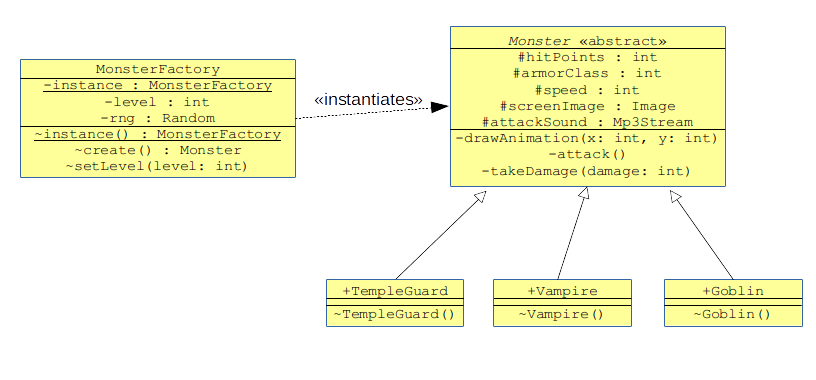
\includegraphics[width=0.9\textwidth]{monsterFactory.pdf}
\caption{The factory pattern in a randomly-generated setting.}
\label{fig:monsterFactory}
\end{figure}

\index{create@\texttt{.create()}}
The Factory pattern makes this easy. All we need to do is encapsulate the
functionality for creating monsters into the \texttt{.create()} method, as
shown in Figure~\ref{fig:monsterFactoryCode}. Then, whenever our program needs
to create a new bad guy, this line of code suffices:

\begin{Verbatim}[fontsize=\small,samepage=true,frame=none]
  Monster newMonster = MonsterFactory.instance().create();
\end{Verbatim}

When the player completes a level and is ready for the next challenge, our
client code simply calls:

\begin{Verbatim}[fontsize=\small,samepage=true,frame=none]
  int currLevel = MonsterFactory.instance().getLevel();
  MonsterFactory.instance().setLevel(currLevel + 1);
\end{Verbatim}

and away we go.

\index{Random.nextDouble@\texttt{Random.nextDouble()}}
\begin{figure}
\begin{Verbatim}[fontsize=\footnotesize,samepage=true,frame=single]
class MonsterFactory {
    private int level;
    private java.util.Random rng;
    
    ...singleton stuff...

    Monster create() {
        Monster m = null;
        switch (level) {
            case 1:
                double randomNumber = rng.nextDouble();
                if (randomNumber < .5) {
                    m = new Goblin();
                } else {
                    m = new TempleGuard();
                }
                m.setHitPoints(rng.nextInt(8));
                m.setArmorClass(rng.nextInt(8));
                m.setSpeed(rng.nextInt(5));
                break;
            case 2:
                double randomNumber = rng.nextDouble();
                if (randomNumber < .4) {
                    m = new Goblin();
                } else if (randomNumber < .8) {
                    m = new TempleGuard();
                } else {
                    m = new Vampire();
                }
                m.setHitPoints(rng.nextInt(8) + 5);
                m.setArmorClass(rng.nextInt(8) + 4);
                m.setSpeed(rng.nextInt(10));
                break;
        }
        return m;
    }
}
\end{Verbatim}
\caption{A factory to generate baddies randomly, based on the game's level.
(Recall the \texttt{java.util.Random} class from Section~\ref{Random} on
p.~\pageref{Random}.)}
\label{fig:monsterFactoryCode}
\end{figure}

Hopefully you're getting the gist, here: if the instantiation process for an
object is a bit complex, it makes sense to separate it into its own class.
This way, you don't have to duplicate the logic in separate places, and you
don't have to clutter your client code with a giant \texttt{switch} or
\texttt{if-else} construct right in the middle of instantiating and using an
object.



\chapter{Team software development}

At some point in your career (perhaps now), you will begin to work on projects
that are too big for any one person to complete in an acceptable amount of
time. The solution, of course, is to work on a \textbf{team} with other
software developers. Working on a team brings up a host of other issues, some
technical and some social.

\section{Team-based version control with \texttt{git}}

\index{git@\texttt{git}}
\index{CLI (command-line interface)}
Waaaay back in \chapref{ch:gettingOff} (p.~\pageref{introduceGit}) I briefly
introduced the \texttt{git} version control system. Hopefully you've been
using it all along to do the simple process of ``committing'' code to your
repo in individual snapshots. This is a habit you'll want to continue to
ingrain in your cerebral cortex. Commits are the building blocks of any
version control system, including \texttt{git}; without them, you don't have
anything to work with.

Now it's time to learn a little more about \texttt{git}, and especially how it
works in a team environment.

\index{repository@``repo'' (repository)}
\index{directory!child}
\index{bleeding edge}
\index{workspace}
\index{vim@\texttt{vim}}
\index{Filbert}
\index{tree}
Figure~\ref{fig:filbertGit} shows the environment you've been using so far: a
single developer, with a single \textbf{repo}. I use the term
\textbf{workspace} to mean ``the directory (and possibly subdirectories) in
which the developer's files actually exist.'' In Figure~\ref{fig:filbertGit},
the developer is Filbert. His workspace is shown as a yellow oval, which
matches the ovals from way back in Figure~\ref{fig:tree}
(p.~\pageref{fig:tree}) that represented ordinary Linux directories. This
yellow oval contains the ``bleeding edge'' of what Filbert is working on: as
soon as he saves any file from \texttt{vim}, the file in that directory is
instantly updated based on what he just typed, warts and all.

\begin{figure}[ht]
\centering
\includegraphics[width=0.4\textwidth]{filbertGit.pdf}
\caption{A single developer's repo and workspace.}
\label{fig:filbertGit}
\end{figure}

\index{git@\texttt{git}!\texttt{.git} directory}
\index{cd@\texttt{cd}}
Filbert's personal git repo is shown as a green box. At this point, you should
view a repo as a sort of ``mysterious'' thing that somehow maintains a record
of all the previous changes to all the project's files, yet in a way you don't
need to understand. Using \texttt{git} commands from the command line is the
only way we will inspect and command it.\footnote{If you're curious, it is
maintained in a hidden directory called ``\texttt{.git}'' -- note the initial
dot -- inside the top-level directory of your workspace. If you \texttt{cd} in
there, you'll see all kinds of crazy stuff under the hood. Do \textit{not}
modify any of it, or you'll probably break your repo and lose all its contents!}

\index{staging area}
\index{git@\texttt{git}!\texttt{git status}}
\index{git@\texttt{git}!\texttt{git add}}
\index{git@\texttt{git}!\texttt{git commit}}
\index{commit}

Also shown is a purple diamond called the \textbf{staging area}. Normally you
don't think too hard about the purple diamond explicitly, but it is there, and
the command ``\texttt{git status}'' will only fully make sense if you recognize
its use. Essentially, the staging area is for changes that the developer is
``about to commit'' (or ``fixin' to commit,'' as they sometimes say in the
South) but hasn't actually pulled the trigger on yet. When you execute the two
commands ``\texttt{git add} filename'' and ``\texttt{git commit -m "My commit
message"}'', back to back, the \texttt{add} puts a snapshot of the change to
the staging area, and \texttt{commit} actually records it in the repo. (If
you're in the habit of using ``\texttt{git commit -a}'' to commit your files,
it effectively does both the add and the commit all in one step.)

\label{commitPitfall}
Beware a common pitfall with ``\texttt{git commit -a}'', though: it only
commits changes to \textit{existing} files, not \textit{new} files. If you
create a brand new \texttt{.java} file in your workspace, representing a new
class, you must explicitly ``\texttt{git add}'' it to your repo before
committing it. I can't tell you how many times one of my colleagues (or myself
*shame*) has broken a build by committing all of their changes \textit{except}
for the new files.

Anyway, just to repeat the basic instructions for reproducing
Figure~\ref{fig:filbertGit}:

\index{mkdir@\texttt{mkdir}}
\index{hairball}
\begin{compactenum}

\item The command ``{\small \texttt{mkdir someDirName}}'' creates the
workspace, under whatever directory you're currently in (which can be seen via
``{\small \texttt{pwd}}'').

\item The command ``{\small \texttt{cd someDirectoryName}}'' actually goes into
that directory (remember that \texttt{mkdir} alone does \textit{not} change
your current directory).

\item The command ``{\small \texttt{git init .}}'' creates the green box and
the purple diamond.

\item You use ``{\small \texttt{vim}}'' to create files like {\small
\texttt{Hairball.java}} and {\small \texttt{Cat.java}} directly in your
workspace (blue rectangles). \item When you want to snapshot the current
version of one of your files, in anticipation of doing a commit, you type
``{\small \texttt{git add nameOfFile}}''. This adds the current contents to the
purple diamond. You can now proceed editing further, or go straight to the
commit.

\item To actually commit, type ``{\small \texttt{git commit -m "My
message"}}''.\footnote{Or, in place of steps 5 \textit{and} 6, you can do the
shortcut operation ``\texttt{git commit -a -m "message"}'', but only
\textit{if} all the files you're changing were already explicitly ``\texttt{git
add}''ed at some point.}

\end{compactenum}

\subsection{Understanding \texttt{git status}}

Two extremely common commands for inspecting your workspace are ``\texttt{git
status}'' and ``\texttt{git log}''. Let's look at each in turn.

\index{git@\texttt{git}!\texttt{git status}}

The {\small \texttt{git status}} command tells you the current state of your
workspace as compared with your repo. The output will look like this:

\begin{Verbatim}[fontsize=\scriptsize,samepage=true,frame=single]
$ git status
On branch master
Changes to be committed:
  (use "git reset HEAD <file>..." to unstage)
    modified:   Cat.java

Changes not staged for commit:
  (use "git add <file>..." to update what will be committed)
  (use "git checkout -- <file>..." to discard changes in directory)
    modified:   Cat.java

Untracked files:
  (use "git add <file>..." to include in what will be committed)
    Cat.class
    Hairball.class
    Hairball.java
\end{Verbatim}

Several things of interest here:

\begin{itemize}

\index{branch}
\item The ``\texttt{On branch master}'' means you're on the main, default code
``trunk.'' Later in your career, you'll discover that you sometimes want to
create \textbf{branch}es, which are independently developed sequences of
changes for some specific purpose. They are normally brought back together and
merged into the trunk at a later time.

\item The output lists \texttt{Cat.java} as a ``change to be committed.'' This
means that an updated version of \texttt{Cat.java} is \textit{in your purple
diamond.} (Refer back to Figure~\ref{fig:filbertGit}.) If we were to follow up
this command with a ``\texttt{git commit}'', that version of \texttt{Cat.java}
would be committed to the repo for posterity.

\item Somewhat weirdly, the output shows \texttt{Cat.java} as being in the
``changes \textit{not} staged for commit'' section as well! What the heck is
going on here -- is \texttt{Cat.java} going to be committed, or not?

The answer to that question is ``both.'' When a file shows up in both lists,
it means there have been several \textit{different} changes to it, only
\textit{some} of which were present the last time a ``\texttt{git add}'' was
performed, and which are therefore in the purple diamond. Other changes to this
same file were made \textit{after} the ``\texttt{git add}'', and so they are
in the yellow oval only. In a moment, I'll teach you how to find out which
changes are in which category. For now, just grasp the fact that the same file
can be in both sections of the ``\texttt{git status}'' output.

\index{untracked file}
\index{file!untracked}
\item The ``untracked'' files are the files in your workspace that
\texttt{git} doesn't yet know about. Looking at this list is a good way to
avoid making the ``oops I did a \texttt{git commit -a} but forgot to add my
new files'' problem I mentioned earlier (p.~\pageref{commitPitfall}). In this
case, \texttt{Hairball.java} is potentially such a file, and this message
reminds us that we may want to ``\texttt{git add}'' it. If we don't, our next
commit will \textit{only} have the (first set of) \texttt{Cat} changes, not
the \texttt{Hairball} changes.

\index{java file@\texttt{.java} file}
\index{class file@\texttt{.class} file}
\index{git@\texttt{git}!\texttt{.gitignore} file}
\item The other entries under ``untracked'' are compiled \texttt{.class}
files, not \texttt{.java} source files. \textbf{Normally, we \textit{want}
those to be untracked}, and so it's actually good that they're not set up as
part of the commit. Some developers, however (myself included) find this
message annoying. The way to fix it is to create a (hidden) file in your
project directory called ``\texttt{.gitignore}''. \textit{All files whose names
match something in the ``\texttt{.gitignore}'' file will be ignored entirely by
\texttt{git}}, and hence not be mentioned in a cries-wolf warning message.

\begin{samepage}
Here's an example \texttt{.gitignore} file, which you can edit like any other
file in \texttt{vim}:

\begin{Verbatim}[fontsize=\small,samepage=true,frame=single]
.gitignore
*.class
\end{Verbatim}
\end{samepage}

There are two lines. The first is a bit of a mind-blower: it's the name of the
\texttt{.gitignore} file itself! By including the line ``\texttt{.gitignore}''
in our \texttt{.gitignore}, we're telling \texttt{git} to not do version
control on \texttt{.gitignore} itself. (Without that, we'll feel like we're
stuck in a Monty Python skit where we create a \texttt{.gitignore} to avoid
annoying warning messages, only for the \texttt{.gitignore} file itself to
cause another annoying warning message.)

The second line says ``also please ignore any file that ends with
\texttt{.class}''. Now, we know that anything that shows up in the ``untracked
files'' section of \texttt{git status} really is something to think hard about.

\item Finally, notice the helpful comments that ``\texttt{git status}''
provides: they're great for telling you exactly how to change things if
necessary. For instance:

\begin{compactitem}

\index{git@\texttt{git}!\texttt{git reset}}
\index{git@\texttt{git}!\texttt{git checkout}}
\item If we decide we don't want to check in that first set of
\texttt{Cat.java} changes after all, we run the command ``\texttt{git reset
HEAD Cat.java}'' to remove it from the purple diamond.

\item If we want \textit{all} our changes in \texttt{Cat.java} to be committed
(the old pre-\texttt{-git-add} ones and the newer ones), we do ``\texttt{git
add Cat.java}'' which will update the purple diamond's copy to match the
workspace.

\item If we decide to actually ditch the \texttt{Cat.java} changes entirely,
the command is ``\texttt{git checkout -{}- Cat.java}'' to discard them.
(Notice the double-hyphen, and also the spaces on either side of it: it's a
weird syntax but you have to use it.)

\end{compactitem}

\end{itemize}

\subsection{Understanding \texttt{git log}}

\index{git@\texttt{git}!\texttt{git log}}
While \texttt{git status} is a detailed look at the present, ``\texttt{git
log}'' is a detailed look at the \textit{past}. With it, we can see the time,
author, and description of every change that's been made during our whole
project.

I personally find the default \texttt{git log} output pretty wordy. It uses
multiple lines per commit, which to me is TMI and fills up my screen too
quickly:

\begin{Verbatim}[fontsize=\footnotesize,samepage=true,frame=single]
$ git log
commit 928ab4924f1c5ddd3b9e2a1c7b507b1b60cf745d
Author: Betty Lou <bettylou@umw.edu>
Date:   2018-11-03

    Fix NPE bug caused by multiple hairballs.

commit 7813b199f40051df14b23a418bce37ccb51a986d
Author: Filbert <filbert@umw.edu>
Date:   2018-11-02

    Add support for multiple, simultaneous hairballs.

commit bdb0fa3071a220bfaccb0d687046e73873a6381d
Author: Betty Lou <bettylou@umw.edu>
Date:   2018-10-21

    Make most setters private.

commit e4471910b8d27c819e4e0df39804ab607cd16c5c
Author: Jezebel <jezebel@umw.edu>
Date:   2018-10-15

    Add Cat.java, Hairball.java.
\end{Verbatim}

\index{hash}
\index{commit hash}
Notice that the entries are in reverse-chronological order (most recent at the
top), which is what you want to get used to. Each five-line section represents
one commit. The big hairy numbers immediately after the word \texttt{commit}
are called the commit's \textbf{hash}. That just means that every commit has a
unique number, randomly/automatically generated by \texttt{git}, so that you
can unambiguously refer to it. (More on why to do this in a moment.)

The \texttt{Author} and \texttt{Date} elements are self-explanatory, and the
rest of the text is the actual message that the developer typed when doing the
\texttt{git commit}.

It turns out that \texttt{git} provides a great deal of fine-grained control
over what this output looks like. (Right away, that tells you that people look
at git logs a \textit{lot} and need them to be just the right format to
quickly cull maximum information from them.) I like mine to be all on one
line, and in color. To do this, I execute the line:

\begin{Verbatim}[fontsize=\scriptsize,samepage=true,frame=none]
$ git config format.pretty "(%h) %Cblue%an%Creset: %Cgreen%s %Creset(%ad)"
\end{Verbatim}

which looks bizarre, but there's a method to its madness. Each one of these
control characters (starting with a ``\texttt{\%}'') specifies a certain piece
of information or formatting. The result, when I type \texttt{git log} is
this:

\definecolor{darkgreen}{rgb}{0,.65,0}
\begin{Verbatim}[commandchars=\\\{\},fontsize=\scriptsize,samepage=true,frame=single]
$ git log
(928ab49) \textcolor{blue}{Betty Lou}: \textcolor{darkgreen}{Fix NPE caused by multiple hairballs.} (2020-11-03)
(7813b19) \textcolor{blue}{Filbert}: \textcolor{darkgreen}{Add support for simultaneous hairballs.} (2020-11-02)
(bdb0fa3) \textcolor{blue}{Betty Lou}: \textcolor{darkgreen}{Make most setters private.} (2020-10-21)
(e447191) \textcolor{blue}{Jezebel}: \textcolor{darkgreen}{Add Cat.java, Hairball.java.} (2020-10-15)
\end{Verbatim}

\index{man@\texttt{man}}
Easier on the eyes, IMO. Run the command ``\texttt{man git config}'' to see
all the options. Btw, you may be wondering what good it does to only list the
first few characters of the commit hash. It turns out that for most commands
that use it, you only have to type the first few characters anyway (just
enough to guarantee uniqueness) and the short version is waaaay easier to look
at.

\subsection{Comparing versions}

\index{diff@\texttt{diff}}
A very common operation for a developer is to compare two versions (of the
code base, or of a single file) to see what changed between them.
Colloquially, comparing two versions of something is called ``\textbf{doing a
diff},'' named after the Linux ``\texttt{diff}'' command. Here's my favorite
way of comparing versions.

\subsubsection{The \texttt{vimdiff} comparison tool}

\index{vimdiff@\texttt{vimdiff}}
\index{git@\texttt{git}!\texttt{git config}}
First, make these changes to your \texttt{git} profile\footnote{By the way,
any time you want to see \textit{all} of your \texttt{git} configuration
settings, you can do so with the command ``\texttt{git config -e -{}-global}''.
It will bring up all your settings in a text file for you to browse in
\texttt{vim}. You can even edit this file directly to make changes to
settings, although be very careful not to mistype anything. Stuff can go
haywire if you do!}:

\begin{Verbatim}[fontsize=\small,samepage=true,frame=none]
$ git config --global merge.tool vimdiff
$ git config --global diff.tool vimdiff
$ git config --global difftool.prompt false
\end{Verbatim}

\index{git@\texttt{git}!\texttt{git difftool}}
This tells \texttt{git} to use the ``\texttt{vimdiff}'' tool to do
side-by-side comparisons. Then, ``\texttt{git difftool}'' is your principal
way of bringing up a comparison. When you run it, you will get a somewhat
strange-looking window that seems to be running \textit{two} copies of
\texttt{vim}: one on the left and one on the right. All your \texttt{vim}
positioning commands -- \texttt{h}, \texttt{j}, \texttt{k}, \texttt{l}, the
arrow keys, \texttt{CTRL-U} and \texttt{CTRL-D}, even search with
``\texttt{/}'' -- move the cursor around just as in normal \texttt{vim}. As
you scroll up or down, both panes will scroll together. The changes from one
version to another will appear in color so you can easily see what's changed
between them. (Note that if there are long sequences of lines that were
unchanged, sometimes \texttt{vimdiff} ``folds them up'' so that it's easier to
skip over them.) 

\begin{figure}
\centering
\hspace*{-.2in}
\includegraphics[width=1.05\textwidth]{catDiff.png}
\vspace{-.05in}
\caption{Using ``\texttt{git difftool}'' when configured with ``\texttt{vimdiff}''.}
\label{fig:catDiff}
\end{figure}

\index{cat.java@\texttt{Cat.java}}
Figure~\ref{fig:catDiff} shows what \texttt{vimdiff} looks like when you run
it. Its vertically-split pane shows two versions of the same file, with the
differences between the two in various colors. It is plain from the figure
that the differences between the two \texttt{Cat.java} versions are:

\index{javadoc@\texttt{javadoc}}
\begin{compactenum}
\item The JavaDoc class comment (see Chapter~\ref{ch:api}) has an extra phrase.
\item A new ``\texttt{breed}'' inst var has been added.
\item A bug has been fixed by changing the ``\texttt{args[1]}'' in the
\texttt{for} loop to ``\texttt{args[0]}''.
\end{compactenum}

Super cool, and easy to see at a glance. Learn to use this often in your
debugging and other code base investigations.

Don't attempt to use \texttt{vimdiff} to \textit{edit} your file, though. If
you're comparing two versions of a file and find a mistake, quit out of
\texttt{vimdiff} and enter plain-ol' \texttt{vim} to fix it. (Incidentally, to
quit \texttt{vimdiff} you have to enter ``\texttt{:q}'' \textit{twice}, once
for each of the panes. Sometimes it's quicker to use the ``\texttt{:qa}'' (for
``quit all'') sequence instead.)

\subsubsection{Specifying the versions to compare}

Okay. So that's how \texttt{vimdiff} (which is triggered from \texttt{git
difftool}) works in general. Now, how do you specify what versions of the
files you want to compare?

If you just type the command with no other arguments:

\begin{Verbatim}[fontsize=\small,samepage=true,frame=none]
$ git difftool
\end{Verbatim}

\index{workspace}
you'll be comparing \textit{your workspace} (yellow oval) against \textit{your
staging area} (purple diamond). This shows you the things that you have
changed \textit{since your last \texttt{git add}}. This is useful when asking,
``I'm about to do a commit...have I forgotten anything I meant to include?''

\index{staged@\texttt{-{}-staged} argument}
If you add the ``\texttt{-{}-staged}'' argument:

\begin{Verbatim}[fontsize=\small,samepage=true,frame=none]
$ git difftool --staged
\end{Verbatim}

\index{staging area}
\index{repository@``repo'' (repository)}
you'll be comparing \textit{your staging area} (purple diamond) with the
\textit{repo} (green box). This is useful when asking, ``if I do a commit
right now, exactly what changes will be recorded?''

\index{commit hash}
\index{hash}
Finally, to compare \textit{any two versions}, include the first few letters
of the commit hash of each. For instance, this command:

\begin{Verbatim}[fontsize=\small,samepage=true,frame=none]
$ git difftool bdb0fa3 7813b19
\end{Verbatim}

\index{Filbert}
will examine the changes Filbert made when he added multi-hairball support.
(Refer to the commit hashes in the \texttt{git log} output, above.) The first
hash identifies the commit Filbert was working with when he began making
changes (\textit{i.e.}, the one he started with), and the second is the hash
of the commit he himself made (the one he ended with). This process gives us
fine-grained resolution in examining the past and identifying errors.

% Rolling back to a previous version (git checkout)


\subsection{Using \texttt{git} with more than one human}

In a team environment, the \texttt{git} tool works much the same way, but with
an added level of complexity to ``join'' the developers together. Look at the
revised picture in Figure~\ref{fig:teamGit}.

\begin{figure}
\centering
\hspace*{-.1in}
\includegraphics[width=1.05\textwidth]{teamGit.pdf}  % 700x550
\caption{A development team's repos and workspaces.}
\label{fig:teamGit}
\end{figure}

\index{Betty Lou}
\index{github}
\index{BitBucket}
We now have two developers working on this feline program: Filbert and his
colleague Betty Lou. The picture is considerably more complex. First, notice
that the three large salmon-colored squares represent \textit{different machines}
which communicate only over the Internet. Filbert and Betty Lou each have
their own laptop to do development on. And in addition, there is a third
machine involved: a publicly-available hosting service like BitBucket,
SourceForge, or github. Think of this public repo as the team's ``home base'':
despite the fact that at any given moment Filbert and Betty Lou may be writing
new code for the project, the latest stable version is always available in the
repo.

There are also some new \texttt{git} verbs we need to learn about to make this
picture work. To wit:

\begin{itemize}
\index{git@\texttt{git}!\texttt{git clone}}
\item \texttt{git clone}: Normally, the way this whole process kicks off is
that someone creates the initial version of the repo on github, and the other
team members \textbf{clone} copies of it. ``Clone'' is exactly what it sounds
like: it means to make an exact duplicate.

\index{git@\texttt{git}!\texttt{git push}}
\index{Microsoft}
github makes it easy to do this in a variety of ways. Perhaps the most common
is when one developer starts with an embryonic version of the code base,
creates his/her own local git repo, and then ``pushes'' (see below) this to a
new github project. It's also possible to start on github with a brand-new
blank project. At the time of this writing, a very helpful and obvious green
``New'' button is present on the github main account screen, with instructions
to follow for each of these different starting techniques.\footnote{Services
like github and BitBucket are free to use, by the way, as long as you keep your
repo public and visible to the world. The idea is that they're trying to
promote open source software, so in exchange for sharing your ideas, they're
giving you free storage space and tools. Some services even have free
\textit{private} repos -- after being purchased by Microsoft, github now offers
this feature for teams with three or fewer developers.}

On the github project page, you'll see a button that says ``Clone or
download,'' and which will display a specific URL to your project if you click
on it. Then, on your local machine, you can go to the directory you want to be
the parent of your project, and type something like:

\begin{Verbatim}[fontsize=\scriptsize,samepage=true,frame=none]
$ git clone https://github.com/stuff/projectName.git projectName
\end{Verbatim}

which will populate your filesystem with a copy of all the repo's files.

\index{git@\texttt{git}!\texttt{git push}}
\item \texttt{git push}: As usual, you'll constantly be making your own local
commits to your own copy of the repo as you work. You should do this every
time you reach a stopping point.

A new operation in the team environment is the ``\texttt{git push}''. It says
``take the updated contents of my own local repo (which have already been
committed) and propagate them up to the team repo in github.'' This is how you
share your changes with your teammates.

\index{git@\texttt{git}!\texttt{git commit}}
\index{commit}
Rule of thumb: making a local \texttt{commit} should be a common operation.
Doing a \texttt{push}, on the other hand, is rarer: you only do it when your
teammates need your latest code, and when your code is stable enough to
warrant making it ``the new normal'' in the team repo.

Last thing on \texttt{git push}: you normally don't do a \texttt{push} until
\textit{after} doing a \texttt{pull} to make sure you have your teammate's
latest code integrated in yours. See next bullet.

\index{git@\texttt{git}!\texttt{git pull}}
\item \texttt{git pull}: The inverse process of \texttt{push} is
\texttt{pull}. It means, ``go to github, fetch whatever changes have been made
by my fellow developers, and integrate them into my repo so I have the latest
and greatest.''

Now here's where \texttt{git} is fancy, and dare I say, seemingly magic.
Suppose you've been editing code for the project at the same time your
teammates are, and furthermore you're actually editing \textit{the same
files}. Doesn't that seem like it would be a nightmare? Doesn't it seem like
you would each be making incompatible changes, and that one person's work is
ultimately doomed to be wiped out by the other person's changes?

\index{merge}
\index{git@\texttt{git}!auto-merge}
That fear is indeed true if you're thinking of your code ``a file at a time.''
But \texttt{git} is smart enough to consider your code ``a \textit{line} at a
time.'' So if Filbert and Betty Lou are both making changes to
\texttt{Hairball.java}, but they're working on \textit{different parts} of
that file, it turns out that git can automatically and intelligently
\textbf{merge} the changes without you even having to worry about it.

When you do a \texttt{git pull} operation, \textit{read the output carefully.}
About 95\% of the time, it will give you a happy message like this:

\begin{Verbatim}[fontsize=\footnotesize,samepage=true,frame=none]
Auto-merging Hairball.java
Merge made by the 'recursive' strategy.
 Hairball.java | 1 +
 1 file changed, 1 insertion(+)
\end{Verbatim}

This is git's way of saying, ``your teammate was editing the same file(s) as
you, but it's chill; I figured out how to put their changes into your copy
without messing up anything you were doing.'' When this first happened to me,
I admit I was fearful, and couldn't comprehend how it could really be smart
enough to integrate those changes without me checking. But I've since learned
to stop worrying and love the bomb, and it really is ``all good.''

The other 5\% of the time, you're not so lucky, and you'll get a sad message
that says:

\begin{Verbatim}[fontsize=\scriptsize,samepage=true,frame=none]
Auto-merging Hairball.java
CONFLICT (content): Merge conflict in Hairball.java
Automatic merge failed; fix conflicts and then commit the result.
\end{Verbatim}

\index{conflict}
\index{git@\texttt{git}!conflict}
This situation is called a \textbf{conflict} and essentially means that you
and your teammate were working in the same \textit{part} of the file and made
incompatible changes. Perhaps one of you changed line 57 in one way, and the
other of you changed line 57 in a different way. Or perhaps one of you changed
line 90, while the other completely deleted lines 85-95. In these cases, git
can't figure out what you want to do, so it throws it back to you and asks you
to manually resolve it.

Resolving it is generally pretty easy. You open up the offending file(s) in
\texttt{vim}, and look for the markers ``$<<<<<$'', ``$=====$'', and
``$>>>>>$''. Here's the kind of thing you'll see:

\begin{Verbatim}[fontsize=\footnotesize,samepage=true,frame=single]
...
<<<<<<< HEAD
 * <tt>Cats</tt> are wonderful creatures that make good 
 * house pets.
=======
 * A <tt>Cat</tt> is a small fuzzy animal that coerces
 * humans into paying enormous sums of money and weekends
 * of labor in exchange for being "cute."
>>>>>>> c6812dcd33b977de0e7f0e9cab1eb1376bcfda88
...
\end{Verbatim}

\index{Slack}
Here's how to decipher that. The lines between the ``$<<<<<$ \texttt{HEAD}''
and the ``$=====$'' are what \textit{you} had in your version of the file. In
this example, you changed the \texttt{Cat} class JavaDoc entirely by rewriting
it in a more feline-friendly way. Meanwhile, your teammate (whose code is
marked between the ``$=====$'' and the ``$>>>>>$ \texttt{c6812...}'') made a
smaller change to that comment, changing ``furry'' to ``fuzzy.'' All that
matters now is what you want to do about these changes. It's your job as a
developer to restore that part of the \texttt{Cat.java} file to be \textit{what
your team wants the code to look like moving forward.} Perhaps you keep your
change, perhaps you keep your teammate's, perhaps it's a combination of both.
But after fixing it up the way it should be (with maybe a phone call or chat
session on Slack with your colleague to make sure you're on the same page), you
will have removed the ``$<<<<<$'' and ``$=====$'' and ``$>>>>>$'' markers and
can ``\texttt{git add}'' and commit your changes. Finally, you can then push
the combined changes to the team repo, and everything goes on hunky dory.

Normally, the only time you end up in the 5\% conflict case (instead of the
95\% auto-merge case) is when you and your teammates aren't communicating well
(or enough). Two developers both editing the same lines of code and not
realizing that the other person is doing it is usually a sign that you need to
work more closely together or be more explicit about who's working on what. A
simple email or text often does the trick.

\end{itemize}

Bottom line: using the \texttt{git} verbs \texttt{add}, \texttt{commit},
\texttt{pull}, and \texttt{push} properly is your key to ensuring your team
has a living, breathing, healthy, working repository of shared code.

Here are the most common pitfalls I see:

\index{git@\texttt{git}!\texttt{git push}}
\index{git@\texttt{git}!\texttt{git pull}}
\index{git@\texttt{git}!\texttt{git stash}}
\index{man@\texttt{man}}
\begin{compactitem} \item Forgetting to do a \texttt{pull} before trying a
\texttt{push}. git won't allow you to \texttt{push} into a repo if you're
out-of-date. You must first \texttt{pull} the recent changes so you're all in
sync, and \textit{then} you can \texttt{push} your new changes to it. \item
Forgetting to do a local \texttt{commit} before trying to \texttt{pull}. git
won't let you pull changes from another repo if you have car parts all over
your own garage. Make sure you check everything in and have a clean local
workspace before doing that.\footnote{An alternative to a full local commit
here is the ``\texttt{git stash}'' command which I've found useful. Doing a
``\texttt{stash}'' is different than a \texttt{commit}, since you're not
actually marking version control with labeled changes. Instead, you're sort of
sweeping stuff under the rug to make your workspace temporarily clean, for the
sake of doing an important \texttt{pull} operation from your teammates. You
can then pull your stuff back out from under your rug and continue. For
details, type ``\texttt{man git stash}'' and read carefully.}

\end{compactitem}

% TODO: Add: "rewinding to old versions" to:
%  - compare
%  - actually permanently roll back



\chapter{Doing design (1 of 2)}
\label{design1}

\index{analysis}
\index{synthesis}
This chapter marks a watershed of sorts. Up to this point, we've been doing
\textbf{analysis} instead of \textbf{synthesis}. Analysis is when you look at
something that already exists -- a design diagram or a code snippet, say --
and seek to understand it, usually by breaking it down into its constituent
parts. Synthesis, on the other hand, is designing something that doesn't
already exist. Instead of scrutinizing a UML diagram, we're creating a UML
diagram; instead of examining a method, we're writing a method.

\index{ballplayer@\texttt{Ballplayer}}
Until now, I've presented you with example after example of classes and
methods already written, and diagrams illustrating their various parts. But
now it's time to ask the question: ``how do we figure out what the right
classes and methods \textit{are} in the first place?'' It's all well and good
for someone to hand us \texttt{Ballplayer}, \texttt{Team}, and
\texttt{Simulator} classes. But how did we know to create those particular
classes? Why not \texttt{Pitch}, \texttt{Catch}, and \texttt{Hit}? Why not
\texttt{FirstBaseman}, \texttt{Shortstop} and \texttt{Outfielder}? Why not
\texttt{NationalLeague} and \texttt{AmericanLeague}?

Going from the general idea of a program to a list of classes is tricky. It's
as much an art as a science. It calls for intuition and imagination more than
adherence to a set of rules. Nevertheless, there are principles that guide the
selection of good classes, and we'll talk about them in this chapter.

\index{Wirfs-Brock, Rebecca}
\index{responsibility-driven design}
Of all the OO pioneers who weighed in on the question of how to arrive at a
good design, the one who had the most influence on me was Rebecca Wirfs-Brock,
who invented the technique called \textbf{responsibility-driven design}. I'm
highly indebted to her, and recommend the original book authored by her and
her colleagues.\footnote{Wirfs-Brock, Wilkerson, Wiener, \textit{Designing
Object-Oriented Software.} Prentice Hall, 1991.}

\section{``Discovering the design''}

\index{discovering the design@``discovering the design''}
I don't know who first coined the phrase ``discovering the design'' (it
certainly wasn't me; it might have been Wirfs-Brock) but when I originally
heard it my ears perked up. It sounded strangely paradoxical. ``Design'' was
something one brought to the table and imposed on one's world, right? Not
something one found already there. ``Design'' seemed like a matter of
\textit{invention}, not \textit{discovery}; it was surely something you did to
a steam engine, not to a planet.

Yet hidden in this phrase is a powerful technique for OO design that attempts
to \textit{let the requirements speak for themselves.} One of Rebecca
Wirfs-Brock's great ideas was to begin with a written description of a
software program in action, and to cull from the language clues as to what the
``correct'' classes are.

Let me immediately clarify that ``correct'' does not mean ``there is one and
only one `right' set of classes'' for a particular program. In fact, there are
many such choices, some better than others, some downright awful. What we
mean by ``the correct classes'' is a set of classes (and their corresponding
inst vars and methods) that will:

\index{responsibilities}
\begin{compactitem}
\item represent the domain well
\item work seamlessly together
\item be amenable to adaptation as the system requirements evolve
\item distribute the responsibilities evenly among several classes
\item neither duplicate nor omit important functionality
\end{compactitem}

You get the picture. A good design is elegant, flexible, maintainable, and
robust to change. Many choices of classes will not meet these goals. A few
will. ``The correct set of classes'' means \textit{any} set of classes that
will do so reasonably well.

\section{Straight from the horse's mouth}
\label{reqSpec}

\index{requirements!specification (``req spec'')}
Wirfs-Brock's procedure is paraphrased in Figure~\ref{fig:discovering}. We
have to somehow come up with a written description to kick things off. Often,
a \textbf{requirements specification}\footnote{Sometimes called a ``req spec''
-- pronounced ``reck speck.''} has been authored by someone higher-up on our
company's food chain, and can be mined for much gold. Sometimes, we ourselves
take a step back and bang out a few paragraphs that describe what users do and
experience as they work with the system.

\setlength{\fboxsep}{10pt}
\begin{figure}
\centering
\fbox{\parbox{.85\textwidth}{
Start with a written description of the software, and:
\begin{compactenum}
\itemsep.03in
\item Identify all noun phrases.
\item Eliminate obviously bad ones:
    \begin{compactenum}
    \item probable duplicates
    \item nouns that aren't instantiate-able
    \item things you obviously wouldn't represent
    \item likely \textit{attributes} of a class, not classes themselves
    \end{compactenum}
\item The remaining ones are your \textbf{candidate classes}. See which of
them ``feel right.'' Identify what each one \textbf{knows} and can \textbf{do}.

\end{compactenum}
}}
\vspace{.1in}
\caption{Procedure for ``discovering the design.''}
\label{fig:discovering}
\end{figure}

The essential point is that the requirements themselves speak loudly about
what classes would be appropriate for the program it describes. Let's see how.

\subsection{Nouns, and only nouns}

\index{noun}
If you flash back to \textit{Schoolhouse Rock} or \textit{Sesame Street},
you'll remember your grammatical parts of speech and realize that a
\textbf{noun} is the right kind of word for a class name. Every object (and
therefore the class it's an instance of) is a ``person, place, or thing,'' not
an action word, modifier, or anything else.

Further, not just not any old noun will do. Consider the list in
Figure~\ref{fig:nouns}: these are all nouns, but only \textit{one} makes a
valid class name. Can you find it?

\setlength{\fboxsep}{1pt}
\begin{figure}[hb]
\centering
\fbox{\parbox{.85\textwidth}{
\begin{multicols}{3}
\begin{compactitem}
\renewcommand\labelitemi{\freakingtilde}
\item happiness
\item Beyonc\'{e}
\item oxygen
\columnbreak
\item crocodile
\item teamwork
\item width
\columnbreak
\item communism
\item recreation
\item London
\end{compactitem}
\end{multicols}
}}
\vspace{.1in}
\caption{All nouns...but not all good class names.}
\label{fig:nouns}
\end{figure}

\index{noun!proper}
I claim the only legit class name in this list is
\underline{\textit{crocodile}}. Here's why. First, some of these entries are
``proper nouns'' which means they refer to specific instances of things, rather
than categories. In English, we almost always use \textit{capital letters} to
denote proper nouns, which means when you see ``Beyonc\'{e}'' and ``London''
you can immediately roll your eyes and move on.

\label{instantiation}
Second, most of the other nouns aren't \textit{instantiate-able}. Here's the
litmus test for whether a noun is instantiate-able: can you meaningfully
put the word ``a'' (or ``an'') before it? And can you meaningfully make it
plural and put a number (like thirteen) before it?

Clearly not. All of these phrases are plainly ridiculous:

\begin{multicols}{2}
\begin{compactitem}
\item four happinesses (?)
\item eleven oxygens\footnote{One could imagine a chemical analysis program
that dealt with oxygen atoms, among other things, and I've heard chemists
speak loosely of things like ``an extra oxygen'' or say ``that molecule has
five oxygens.'' I still like \texttt{OxygenAtom} much, much better as a class
name even here, though.} (?)
\item a teamwork (?)
\columnbreak
\item a communism (?)
\item nineteen recreations (?)
\end{compactitem}
\end{multicols}

Remember, the only thing we ever really do to a class is make instances of it,
to which we can do things. If you can't imagine a ``\texttt{new Communism()}''
or ``an \texttt{ArrayList} of \texttt{Happiness}es,'' it has no business being
a class.

The closest contender to crocodile is the word \textit{width}. There may be
cases where this is a sensible class, but the reason I discard it is that a
width is almost certainly a \textit{modifier} of some other object, rather
than an object itself. One could imagine \texttt{Building}, \texttt{Image},
and \texttt{Rectangle} objects that all had an instance variable called
\texttt{width}; it's harder to imagine ``a width'' as an entity in its own
right, with its own properties and operations.

\subsubsection{Noun phrases}

\index{noun!noun phrase}
By the way, it's often the case that instead of a bare noun, we use a
\textbf{noun phrase} as a class name. A noun phrase is simply a noun with one
or more modifiers. ``Grizzly bear,'' ``chess tournament,'' and ``public liberal
arts college'' are examples.

\subsubsection{Singular, not plural}

\index{noun!singular}
Finally, it should hardly be worth stating that all class names must be
\textbf{singular}, not plural. I don't work in ``a buildings,'' but a
\textit{building}; and nobody has ``a dogs'' as a pet. When we instantiate an
object, we're going to say ``\texttt{Crocodile alice = new Crocodile()}'', not 
``\texttt{Crocodiles alice = new Crocodiles()}''.

\section{Carrying out the process}

\textbf{1. Identify all noun phrases.} Okay. We begin our semi-automated
process of deriving class names by starting with a written description of the
program's requirements. Here's a short example:

\index{bicycle}
\setlength{\fboxsep}{10pt}
\begin{center}
\label{blockRequirements1}
\large
\fbox{\parbox{.85\textwidth}{
\textsf{A bicycle store needs to manage its inventory. Shipments of various
models of bicycles are received every week from its suppliers, and customers
place individual orders for bikes and other accessories from the store. The
store manager must be able to place orders from vendors, maintain
contact information so they can be confirmed or canceled, and view lists of
the incoming products and their expected arrival dates. The manager also must
be able to record multi-item orders from individual customers, accept and
record down payments, and track inventory levels to ensure that enough items
are ordered to satisfy customer demand.}}}
\end{center}

Rebecca Wirfs-Brock's process from Figure~\ref{fig:discovering} calls for
sifting through the requirements description and \textit{circling all the noun
phrases}. Unless it's an exact duplicate of one that previously occurred, be
conservative and circle every one. It would be a good exercise for you to do
this yourself in the box above, and then compare with my answer:

\setlength{\fboxsep}{10pt}
\begin{center}
\large
\fbox{\parbox{.85\textwidth}{
\textsf{A \bluebox{bicycle store} needs to manage its \bluebox{inventory.}
\bluebox{Shipments} of various
\bluebox{models} of \bluebox{bicycles} are received every \bluebox{week} from its
\bluebox{suppliers}, and \bluebox{customers}
place \bluebox{individual orders} for \bluebox{bikes} and other
\bluebox{accessories} from the \bluebox{store}. The
\bluebox{store manager} must be able to place \bluebox{orders} from
\bluebox{vendors}, maintain
\bluebox{contact information} so they can be confirmed or canceled, and view
\bluebox{lists} of
the \bluebox{incoming products} and their \bluebox{expected arrival dates}. The
\bluebox{manager} also must
be able to record \bluebox{multi-item orders} from \bluebox{individual
customers}, accept and
record \bluebox{down payments}, and track \bluebox{inventory levels} to ensure
that enough \bluebox{items}
are ordered to satisfy \bluebox{customer demand}.}}}
\end{center}

This is the raw material for the rest of the process. If we make everything
singular and lower-case, this leaves us with the following list:

\begin{samepage}
\begin{multicols}{3}
\small
\begin{compactitem}
\renewcommand\labelitemi{\raisebox{0.25ex}{\tiny$\bullet$}}
\item \textsf{bicycle store}
\item \textsf{inventory}
\item \textsf{shipment}
\item \textsf{model}
\item \textsf{bicycle}
\item \textsf{week}
\item \textsf{supplier}
\item \textsf{customer}
\item \textsf{individual order}
\columnbreak
\item \textsf{bike}
\item \textsf{accessory}
\item \textsf{store}
\item \textsf{store manager}
\item \textsf{order}
\item \textsf{vendor}
\item \textsf{contact information}
\item \textsf{list}
\item \textsf{incoming product}
\columnbreak
\item \textsf{expected arrival date}
\item \textsf{manager}
\item \textsf{multi-item order}
\item \textsf{individual customer}
\item \textsf{down payment}
\item \textsf{inventory level}
\item \textsf{item}
\item \textsf{customer demand}
\end{compactitem}
\end{multicols}
\end{samepage}

\textbf{2a. Eliminate probable duplicates.} According to
Figure~\ref{fig:discovering}, the next step is to eliminate likely duplicates.
Obviously things like ``bicycle'' and ``bike'' refer to the same conceptual
entity; we're hardly going to have a \texttt{Bicycle} class and a separate
\texttt{Bike} class in our program!

This isn't always 100\% straightforward, but it's usually 99\% so. Different
synonyms and turns of phrase are pretty easy to detect. I think we can be
pretty safe boiling this list down into a slightly smaller one, where
duplicates are shown:

\begin{samepage}
\begin{multicols}{2}
\small
\begin{compactitem}
\renewcommand\labelitemi{\raisebox{0.25ex}{\small$\bullet$}}
\item \textsf{bicycle store == store}
\item \textsf{inventory}
\item \textsf{shipment}
\item \textsf{model}
\item \textsf{bicycle == bike}
\item \textsf{week}
\item \textsf{supplier == vendor}
\item \textsf{customer == individual customer}
\item \textsf{individual order == order == multi-item order}
\columnbreak
\item \textsf{accessory}
\item \textsf{store manager == manager}
\item \textsf{contact information}
\item \textsf{list}
\item \textsf{incoming product}
\item \textsf{expected arrival date}
\item \textsf{down payment}
\item \textsf{inventory level}
\item \textsf{item}
\item \textsf{customer demand}
\end{compactitem}
\end{multicols}
\end{samepage}

The choice of which synonym to retain is mostly aesthetic. All other things
being equal, I usually choose the shorter one.

\vspace{.3in}
\index{instantiation}
\textbf{2b. Eliminate nouns that aren't instantiate-able.} Now we apply our
test: ``can we put `a/an' or a number before the noun phrase, and have it make
sense?''

Actually almost all of these remaining entries pass that test, with the
exception of \textsf{customer demand}, and possibly \textsf{contact
information}. While one could indeed envision ``four or five customer demands''
in other contexts, it's pretty clear from the text that this is being used as
an abstract concept, not an individual object. ``Contact information'' is a
closer call, but by inspecting the requirements again, we can see that this is
really an attribute of \textsf{vendor/supplier}. We'll therefore strike the
idea of a ``\texttt{ContactInformation}'' class. We're now down to:

\begin{multicols}{3}
\small
\begin{compactitem}
\item \textsf{store}
\item \textsf{inventory}
\item \textsf{shipment}
\item \textsf{model}
\item \textsf{bicycle}
\item \textsf{week}
\columnbreak
\item \textsf{supplier}
\item \textsf{customer}
\item \textsf{order}
\item \textsf{accessory}
\item \textsf{manager}
\columnbreak
\item \textsf{list}
\item \textsf{incoming product}
\item \textsf{expected arrival date}
\item \textsf{down payment}
\item \textsf{inventory level}
\item \textsf{item}
\end{compactitem}
\end{multicols}


\textbf{2c. Eliminate things you obviously wouldn't represent.} When you look
at some of these surviving noun phrases, you scratch your head. Would we
really have a ``\texttt{Week}'' class? Surely not. Also, although this program
will no doubt be used by the manager of a store, does it really make sense to
represent the \texttt{Manager} as an object? We'll cross out both of these.

\vspace{.2in}

\textbf{2d. Eliminate likely \textit{attributes} of a class.} Things are
getting a bit more subjective, but some of these remaining nouns definitely
seem ``too small'' to be their own classes. Consider \textsf{expected arrival
date}. Surely this is better modeled as a property of an order, rather than as
its own individual object. The same could be said for \textsf{down payment} and
\textsf{inventory level}. Generally speaking, noun phrases that seem to refer
to bits of data that have an obvious ``home'' in another class ought to be
modeled as inst vars, not classes.

So now here's all that remains:

\vspace{-.2in}
\begin{samepage}
\begin{center}
\parbox{.8\textwidth}{
\begin{multicols}{2}
\begin{compactitem}
\item \textsf{store}
\item \textsf{inventory}
\item \textsf{shipment}
\item \textsf{model}
\item \textsf{bicycle}
\item \textsf{supplier}
\columnbreak
\item \textsf{customer}
\item \textsf{order}
\item \textsf{accessory}
\item \textsf{list}
\item \textsf{incoming product}
\item \textsf{item}
\end{compactitem}
\end{multicols}
}
\end{center}
\end{samepage}
\vspace{-.1in}

\label{candidate class}
We dub these our \textbf{candidate classes}, which essentially means ``those
noun phrases which each have a very good chance of actually turning into a
class in our program.'' We're not 100\% committed to them yet, but they pass
muster enough to deserve a deep think.

\vspace{.3in}

\pagebreak
\textbf{3a. See which of the remaining ones ``feel right.''} We've come a long
way semi-mechanically. Now it's time to allow ourselves the luxury of turning
over in our minds each candidate class, ``trying it on,'' so to speak. 

It's here that a clear picture of our software system emerges. When I look at
the ten candidate classes, here's what comes to mind:

\begin{itemize}
\itemsep.1em

\index{requirements!specification (``req spec'')}
\item First, and most importantly, I realize that the word ``order'' was used
in \textit{two different ways} in the requirements description. You may have
actually noticed this earlier when we scratched out ``expected arrival date''
and ``down payment'' in step 2d. Those were both aspects of an order...but what
\textit{sort} of order? If we go back to the Bible (the req spec) we see these
two phrases:

\begin{quote}
\textsf{``...customers place individual orders for bikes and other accessories
from the store...''}
\end{quote}

\vspace{-.3in}
\begin{center}
and
\end{center}
\vspace{-.2in}

\begin{quote}
\textsf{``...The store manager must be able to place orders from vendors...''}
\end{quote}

Aha! Different beasts entirely. One is something Mrs.~Jamison places with
\textit{us};
the other is something \textit{we} place with Schwinn, Inc.

This sort of post-noun-phrase-stage epiphany isn't uncommon. English words are
used in a variety of ways, which makes them versatile and suggestive, yet
imprecise. Here, we clearly have two different notions of ``order'': (1) a
contract for delivery from one of our big suppliers like Trek or Cannondale
(which might include a dozen bikes or more), and (2) a customer's reservation
of a particular model/color/style of bike, which he or she is anxiously
waiting to take home for its first ride. More succinctly: one kind we buy, and
the other kind we sell.

We're going to have to invent at least one noun phrase of our own here, since
the req spec author double-dipped on the word ``order''; perhaps we'll call the
first one a \texttt{PurchaseOrder} and the second one a
\texttt{CustomerRequest}. (In situations like this, I think it's better to
\textit{avoid} using the original word altogether, since it was ambiguous to
begin with and therefore may encourage confusion down the road.)

\index{inheritance}
\item Second, I notice that some of these nouns have overlapping meanings, and
I sense that \textit{inheritance} might be applicable. In particular, consider
these four noun phrases:

\begin{quote}
\begin{center}
\textsf{bicycle \quad \quad \quad accessory \quad \quad \quad incoming product
\quad \quad \quad
item}
\end{center}
\end{quote}

These clearly all refer to things that can be purchased. When we go back to the
Bible, we see that the modifier ``\textsf{incoming}'' on \textsf{product}
really refers to the temporary state of a product (\textit{i.e.}, one in
transit from a supplier), not a fundamentally distinct kind of thing. So I'm
going to be bold, ditch ``incoming,'' and make these two assertions:

\begin{compactenum}
\item \textsf{item == product}
\item \textsf{bicycle} and \textsf{accessory} are two different kinds
(subclasses) of \textsf{item}
\end{compactenum}

\end{itemize}

With these changes, our list is now:
\vspace{-.2in}
\begin{samepage}
\begin{center}
\parbox{.9\textwidth}{
\begin{multicols}{2}
\begin{compactitem}
\item \textsf{store}
\item \textsf{inventory}
\item \textsf{shipment}
\item \textsf{model}
\item \textsf{bicycle} (subclass of \textsf{item})
\item \textsf{supplier}
\columnbreak
\item \textsf{customer}
\item \textsf{purchase order}
\item \textsf{customer request}
\item \textsf{accessory} (subclass of \textsf{item})
\item \textsf{list}
\item \textsf{item}
\end{compactitem}
\end{multicols}
}
\end{center}
\end{samepage}

\vspace{.1in}


\textbf{3b. Identify what each one \textit{knows} and can \textit{do}.}

\index{encapsulation}
\index{state}
\index{behavior}
As you'll recall from Chapter~\ref{ch:encapsulation}, a well-conceived class
combines both \textbf{state} and related \textbf{behavior}. This is the
cornerstone of good object-oriented design.

\index{CRC card}
Hence at this stage, we apply this litmus test to the candidate classes that
remain. One tool to facilitate this procedure is creating a set of \textbf{CRC
cards}, which stands for ``Class, Responsibilities, Collaborations.'' The idea
is for your design team to create a literal $3\times5$ card for each candidate
class, put them on a flat workspace so you can move them around and compare
and group them, and see whether they seem to fit into a cohesive whole.

\index{class@\texttt{class}}
\index{responsibilities}
\index{collaborations}
The \textbf{Class} for each card is just the class name (which can be fluid as
you try to zero in on the best name). The \textbf{Responsibilities} include the
state (``what an object of that type knows'') and the behavior (``what an
object can do''), which I usually designate in separate sections. Finally, the
\textbf{Collaborations} are the other classes the class is likely to work
closely with to accomplish its job.

If you try to make a CRC card for a class, and have trouble coming up with
appropriate contents (particularly the Responsibilities section), that's a red
flag that perhaps this isn't a good class after all.

\pagebreak
\begin{samepage}
Let's start at the top.

\bigskip
\label{bikeCRC1}
\index{shipment@\texttt{Shipment}}
\begin{center}
\begin{tabular}{|l|}
\hline
\texttt{Shipment}:\\
\hline
\begin{tabular}{rl}
\textit{Knows}: & which vendor is delivering it\\
& which purchase order it is fulfilling\\
& the expected arrival date\\
& the items in each shipment \\
\textit{Can}: & receive and add to inventory\\
& cancel \\
& update status \\
\hline
\textit{Collaborates}: & \texttt{PurchaseOrder}, \texttt{Item}, \texttt{Inventory}, \texttt{Supplier}\\
\end{tabular}\\
\hline
\end{tabular}
\end{center}
\end{samepage}
\bigskip

Our \texttt{Shipment} class looks like a good one. It clearly bears the
hallmarks of good OO design: it has state (information about what's in the
shipment, when it's due, and who it's from) and associated behavior (accept
it, cancel it, get an updated status).

You might be thinking, ``that's great, Stephen, but how did you know what to
write in that box?'' I admit it's not a turn-the-crank process. This is part of
the design process that's art, not science. Basically, though, you have to try
to create a little egocentric world in your mind, the center of which is the
class in question. 

Here, I said to myself, ``let's view the entire world through the lens of a
Shipment. First, in the real world, what ought a shipment to `\textit{know}'?''
The answer is things that relate directly to that shipment. The items it should
contain and the expected date of receipt are good examples. The number of
bicycles in the store is not, nor is a customer's contact information. Then, I
asked ``in the real world, what \textit{actions} pertain to a shipment?'' The
main one, of course, is to receive that shipment, which involves paying for it
and adding the items to the store. We also might ask the supplier for an update
if the shipment is past date, or even decide to cancel it and go with another
vendor if it's taking too long.

The important thing here isn't to get all the ``knows'' and ``cans'' 100\%
right -- things will evolve as our understanding evolves. It's more important
to recognize that there \textit{are} clear ``knows'' and ``cans'' for this
class, which certifies it as a bona fide entity within our object-oriented
system.

The ``Collaborates:'' list consists of those other classes we've identified as
likely co-participants in various system functions. A \texttt{Shipment} is
related to a \texttt{PurchaseOrder}, of course, since the former is the
fulfillment of the latter. Its also comprised of \texttt{Item}s, and will need
to update the \texttt{Inventory} levels when it arrives. It may need to call
methods directly on the \texttt{Supplier} class in the case where updates or
cancellations are necessary. Often the collaborations list just helps us
organize our thoughts (and our $3\times5$ cards) by grouping related classes
together.

Let's walk through a couple of other CRC cards.

\bigskip
\label{bikeCRC2}
\index{accessory@\texttt{Accessory}}
\begin{center}
\begin{tabular}{|l|}
\hline
\texttt{Accessory}:\\
\hline
\begin{tabular}{rl}
\textit{Knows}: & its name\\
& its manufacturer\\
& its part \#\\
& its cost \\
& its compatible bicycle models \\
\textit{Can}: & purchase \\
& find quantity in stock\\
& add to customer request  \\
\hline
\textit{Collaborates}: & \texttt{CustomerRequest}, \texttt{Model}, \texttt{Inventory}\\
\end{tabular}\\
\hline
\end{tabular}
\end{center}
\bigskip

An \texttt{Accessory} -- which we've tentatively identified as a subclass of
\texttt{Item} -- has attributes like name and cost, and also knows which bike
models (if any) it is compatible with. This prevents a customer from ordering
the wrong kind of bike seat or fender for a particular bicycle, for instance.
It can also be purchased (duh), either on the spot or as part of a special
customer order. It can also provide its quantity information by interfacing
with the \texttt{Inventory} class. Speaking of which...

\bigskip
\index{inventory@\texttt{Inventory}}
\begin{center}
\begin{tabular}{|l|}
\hline
\texttt{Inventory}:\\
\hline
\begin{tabular}{rl}
\textit{Knows}: & the quantity of each item in the store \\
\textit{Can}: & add items when shipments arrive \\
& remove items when purchases are made \\
& find quantity in stock \\
\hline
\textit{Collaborates}: & \texttt{Item} (and subclasses)\\
\end{tabular}\\
\hline
\end{tabular}
\end{center}
\bigskip

\index{Singleton pattern}
\index{design pattern!Singleton}
I smell a Singleton. Our store is likely going to have a single
\texttt{Inventory} object which can be used to query and update its item
quantities.

By the way, you may have noticed that one of the ``Can'' items --
``find quantity in stock'' -- was listed on the CRC card for both
\texttt{Accessory} and \texttt{Inventory}. This isn't wrong; probably an
\texttt{Accessory} object, when asked for its current quantity, will turn
around and query the \texttt{Inventory} singleton to produce that answer.
We've discovered a key shared function between classes.

That's the inventory of the store, and now for the \texttt{Store} itself:

\bigskip
\index{store@\texttt{Store}}
\begin{center}
\begin{tabular}{|l|}
\hline
\texttt{Store}:\\
\hline
\begin{tabular}{rl}
\textit{Knows}: & its inventory \\
\textit{Can}: & ? \\
\hline
\textit{Collaborates}: & \texttt{Inventory} \\
\end{tabular}\\
\hline
\end{tabular}
\end{center}

\bigskip
If we didn't realize it before, this is the moment when we discover that our
\texttt{Store} class is weak sauce. Turns out there really isn't anything for
a \texttt{Store} object to know or do, other than manage its inventory, which
of course is the job of the \texttt{Inventory} class. The CRC card process
revealed a false infiltrator, and we discard (literally) the \texttt{Store}.

\index{modularity}
You get the idea. I'll leave the other CRC cards as an exercise for the
reader. Remember, there are no hard-and-fast right answers to this process:
many different designs are possible, and it's only important to get a set of
classes that are cohesive, modular, encapsulated, and work well together.


\vspace{2.8in}

\pagebreak

\section{A longer example}

\index{requirements!specification (``req spec'')}
\index{Uno"!\textsuperscript{\textregistered}}
Figure~\ref{fig:uno} gives a second, longer example of a req spec. We'll
develop this example in the remainder of this chapter and in the next one. In
particular, it involves a non-trivial inheritance hierarchy.

First, test yourself on identifying noun phrases, and see if you find the same
ones marked in Figure~\ref{fig:unoNouns}.

\begin{figure}[hb]
\label{blockRequirements2}
\centering
\small
\setlength{\fboxsep}{10pt}
\fbox{\parbox{.91\textwidth}{

\textsf{To test his intro student's algorithmic development skills, a professor
is developing an Uno!\textsuperscript{\textregistered} simulation program. The
simulator simulates a number of consecutive Uno games, each of which has four
players participating in it. Students write their own Player classes, which are
called by the simulator in order to play cards and call colors after wilds are
played.}

\vspace{.1in}

\textsf{Uno is a game played with a special deck of cards of various types.
Most cards have a color (red, blue, yellow, or green) and feature either a
number on them (from 0 to 9) or else a special action (like ``reverse,''
``skip,'' \textit{etc.}) Some cards are ``wild'' cards, which do not have any
particular color, and thus can be played at any time.}

\vspace{.1in}

\textsf{When play begins, the deck is shuffled, cards are dealt to each
player's hand, and one card is turned face up in the middle of the virtual
table, called the ``up card.'' Each player in turn gets a chance to play, by
playing a card from their hand on top of the up card. That up card is then
replaced by the new up card. If the deck is ever exhausted (\textit{i.e.},
runs out of cards) the discarded cards are reshuffled and placed beside the up
card to be drawn anew. The object of the game is to be the first player to
``go out'' by playing all cards from your hand.}

\vspace{.1in}

\textsf{In order to be legally played, a card must match according to certain
rules (either the color of the card played, or the rank of the card played,
must match the up card.) Some cards have special effects, involving reversing
the direction of play, skipping over player's turns, or causing unfortunate
players to have to draw additional cards from the deck.}

\vspace{.1in}

\textsf{When one player wins a round, he/she gets awarded points based on the
cards remaining in other players' hands. Each type of card has ``forfeit
cost,'' or point value that determines how much it is worth. As it runs, the
simulator maintains the cumulative scores of the players as they each win
games, so that at the end of 50,000 games, an overall winner can be declared.}
}}

\vspace{.1in}
\caption{The requirements specification for a game simulator.}
\label{fig:uno}
\end{figure}

\pagebreak

\begin{figure}
\centering
\small
\setlength{\fboxsep}{10pt}
\fbox{\parbox{1\textwidth}{

\textsf{To test his \bluebox{intro student}'s algorithmic development
\bluebox{skills}, a \bluebox{professor} is developing an \bluebox{Uno
simulation program}. The \bluebox{simulator} simulates a number of consecutive
\bluebox{Uno games}, each of which has four \bluebox{players} participating in
it. \bluebox{Students} write their own \bluebox{Player classes}, which are
called by the simulator in order to play \bluebox{cards} and call
\bluebox{colors} after \bluebox{wilds} are played.}

\vspace{.1in}

\textsf{Uno is a \bluebox{game} played with a special \bluebox{deck} of cards
of various \bluebox{types}. Most cards have a color (red, blue, yellow, or
green) and feature either a \bluebox{number} on them (from 0 to 9) or else a
special \bluebox{action} (like ``reverse,'' ``skip,'' \textit{etc.}) Some cards
are \bluebox{``wild'' cards}, which do not have any particular color, and thus
can be played at any \bluebox{time}.}

\vspace{.1in}

\textsf{When play begins, the deck is shuffled, cards are dealt to each
player's \bluebox{hand}, and one card is turned face up in the middle of the
\bluebox{virtual table}, called the ``\bluebox{up card}.'' Each player in turn
gets a \bluebox{chance} to play, by playing a card from their hand on top of
the up card. That up card is then replaced by the new up card. If the deck is
ever exhausted (\textit{i.e.}, runs out of cards) the \bluebox{discarded
cards} are reshuffled and placed beside the up card to be drawn anew. The
\bluebox{object} of the game is to be the first player to ``go out'' by playing
all cards from your hand.}

\vspace{.1in}

\textsf{In order to be legally played, a card must match according to certain
\bluebox{rules} (either the color of the card played, or the \bluebox{rank} of
the card played, must match the up card.) Some cards have \bluebox{special
effects}, involving reversing the \bluebox{direction of play}, skipping over
player's \bluebox{turns}, or causing \bluebox{unfortunate players} to have to
draw additional cards from the deck.}

\vspace{.1in}

\textsf{When one player wins a \bluebox{round}, he/she gets awarded
\bluebox{points} based on the cards remaining in other players' hands. Each
type of card has ``\bluebox{forfeit cost},'' or \bluebox{point value} that
determines how much it is worth. As it runs, the simulator maintains the
\bluebox{cumulative scores} of the players as they each win games, so that at
the end of 50,000 games, an overall \bluebox{winner} can be declared.} }}

\vspace{.1in}
\caption{Noun phrases.}
\label{fig:unoNouns}
\end{figure}

Our mechanical noun phrase extraction produces this list:

\begin{samepage}
\begin{multicols}{3}
\small
\begin{compactitem}
\renewcommand\labelitemi{\raisebox{0.25ex}{\tiny$\bullet$}}
\item \textsf{intro student}
\item \textsf{skill}
\item \textsf{professor}
\item \textsf{Uno simulation program}
\item \textsf{simulator}
\item \textsf{Uno game}
\item \textsf{player}
\item \textsf{student}
\item \texttt{Player} \textsf{class}
\item \textsf{card}
\item \textsf{color}
\item \textsf{wild}
\columnbreak
\item \textsf{game}
\item \textsf{deck}
\item \textsf{type}
\item \textsf{number}
\item \textsf{``wild'' card}
\item \textsf{time}
\item \textsf{hand}
\item \textsf{virtual table}
\item \textsf{``up'' card}
\item \textsf{chance}
\item \textsf{discarded card}
\item \textsf{object}
\columnbreak
\item \textsf{rule}
\item \textsf{rank}
\item \textsf{special effect}
\item \textsf{direction of play}
\item \textsf{turn}
\item \textsf{unfortunate player}
\item \textsf{round}
\item \textsf{point}
\item \textsf{``forfeit cost''}
\item \textsf{point value}
\item \textsf{cumulative score}
\item \textsf{winner}
\end{compactitem}
\end{multicols}
\end{samepage}

Note that this req spec somewhat unusually refers to a specific
object-oriented \textit{class} (\texttt{Player}) which will of course become
one of our actual classes in the end.

\vspace{.1in}
\textbf{2a. Eliminate probable duplicates.} After eliminating likely
duplicates, our list is shrunk to:

\begin{samepage}
\begin{multicols}{3}
\small
\begin{compactitem}
\renewcommand\labelitemi{\raisebox{0.25ex}{\tiny$\bullet$}}
\item \textsf{student}
\item \textsf{skill}
\item \textsf{professor}
\item \textsf{simulator}
\item \textsf{game}
\item \textsf{player}
\item \textsf{card}
\item \textsf{color}
\item \textsf{``wild'' card}
\columnbreak
\item \textsf{deck}
\item \textsf{type}
\item \textsf{number}
\item \textsf{time}
\item \textsf{hand}
\item \textsf{virtual table}
\item \textsf{``up'' card}
\item \textsf{chance}
\item \textsf{object}
\columnbreak
\item \textsf{rule}
\item \textsf{rank}
\item \textsf{special effect}
\item \textsf{direction of play}
\item \textsf{turn}
\item \textsf{point}
\item \textsf{``forfeit cost''}
\item \textsf{cumulative score}
\end{compactitem}
\end{multicols}
\end{samepage}

An interesting decision here involved the terms \textsf{game} and
\textsf{round}. The former is used in a couple of different senses: Uno itself
is a ``game,'' yet the word ``game'' is also used to mean a single deal of the
cards, at the end of which one player goes out. Curiously, there's no noun in
the description for ``the overall match'' which comprises 50,000 games. We may
find we need such a class. In any event, I scratched \textsf{round} in favor
of \textsf{game} in the list above.

\vspace{.1in}
\textbf{2b. Eliminate nouns that aren't instantiate-able.} After getting rid
of the non-instantiate-able stuff, we shrink further to:

\begin{samepage}
\begin{multicols}{3}
\small
\begin{compactitem}
\renewcommand\labelitemi{\raisebox{0.25ex}{\tiny$\bullet$}}
\item \textsf{student}
\item \textsf{professor}
\item \textsf{simulator}
\item \textsf{game}
\item \textsf{player}
\item \textsf{card}
\item \textsf{color}
\columnbreak
\item \textsf{``wild'' card}
\item \textsf{deck}
\item \textsf{type}
\item \textsf{number}
\item \textsf{hand}
\item \textsf{virtual table}
\item \textsf{``up'' card}
\columnbreak
\item \textsf{rank}
\item \textsf{special effect}
\item \textsf{direction of play}
\item \textsf{turn}
\item \textsf{point}
\item \textsf{``forfeit cost''}
\item \textsf{cumulative score}
\end{compactitem}
\end{multicols}
\end{samepage}

It's worth drawing attention here to the noun ``\textsf{rule},'' which I
discarded. I find that many students' inclination is to keep \textsf{rule} as
a class, whereas I think the description makes it clear that ``rules in
general, according to which the game is played'' is what's intended. And that
would steer us away from instantiating some number of \texttt{Rule} objects.

\vspace{.1in}
\pagebreak
\textbf{2c. Eliminate things you obviously wouldn't represent.} The only ones
I got rid of on this step were (ironically) \textsf{student} and
\textsf{professor}. Nothing personal.

\vspace{.1in}
\textbf{2d. Eliminate likely \textit{attributes} of a class.} I think you'll
agree that \textsf{color}, \textsf{type}, \textsf{number}, and \textsf{rank}
are best suited as attributes of a \texttt{Card} class, not as classes in
their own right. Too, \textsf{direction of play} -- which is simply
``clockwise'' or ``counter-clockwise'' -- seems like a property of the
\textsf{game}. Similar thinking leads to deleting \textsf{point} and
\textsf{cumulative score} (attributes of the \texttt{Player}s) and
\textsf{forfeit cost} (an attribute of a \texttt{Card}.) We're now left with
only:

\begin{samepage}
\begin{multicols}{3}
\small
\begin{compactitem}
\renewcommand\labelitemi{\raisebox{0.25ex}{\tiny$\bullet$}}
\item \textsf{simulator}
\item \textsf{game}
\item \textsf{player}
\item \textsf{card}
\columnbreak
\item \textsf{``wild'' card}
\item \textsf{deck}
\item \textsf{hand}
\item \textsf{virtual table}
\columnbreak
\item \textsf{``up'' card}
\item \textsf{special effect}
\item \textsf{turn}
\end{compactitem}
\end{multicols}
\end{samepage}


\textbf{3a. See which of the remaining ones ``feel right.''} This is honestly a
pretty darn good list. If I were to nitpick it further, I'd probably say that
\textsf{``up'' card} will probably turn out to be an instance variable of
\textit{type} \texttt{Card}, rather than its own class. I'd wager that
\textsf{turn} doesn't end up being a full-blown class either, since ``whose
turn it is'' is better served with an inst var.

The \textsf{``wild'' card} noun phrase is quite literally going to become a
wild card for us, as we'll discover in the next chapter. It conceals what is
really going to be a deep inheritance hierarchy, in which the different types
of cards are all subclasses of \texttt{Card}. This is where the
\textsf{special effect}s come into play as well -- in the end, I didn't model
this as its own class, but rather embedded the functionality into the
\texttt{Card} subclasses. Either way's okay, though.

\vspace{.1in}
\textbf{3b. Identify what each one \textit{knows} and can \textit{do}.}
I'll sign off this chapter by taking a crack at CRC cards for some of the
classes that are going to survive the whole design vetting. These are quality
classes that will ensure a solid design that's robust for the present and the
future!

\index{CRC card}
\label{unoCRC1}
\index{simulation@\texttt{Simulation}}
\small
\begin{center}
\begin{tabular}{|l|}
\hline
\texttt{Simulation}:\\
\hline
\begin{tabular}{rl}
\textit{Knows}: & the name of each player \\
& the \texttt{Player} subclass for each player \\
& how many total games to simulate \\
& how many games have been played so far \\
\textit{Can}: & play some number of games and compute final scores \\
\hline
\textit{Collaborates}: & \texttt{Game}, \texttt{Player} (and subclasses)\\
\end{tabular}\\
\hline
\end{tabular}
\end{center}

\index{card@\texttt{Card}}
\begin{center}
\begin{tabular}{|l|}
\hline
\texttt{Card}:\\
\hline
\begin{tabular}{rl}
\textit{Knows}: & its type \\
& its color (if applicable) \\
& its number (if applicable) \\
& its ``forfeit cost'' \\
& whether it can be legally played on an up card \\
& whether the player who played it can call a new color \\
\textit{Can}: & perform any special effect appropriate to its type \\
\hline
\textit{Collaborates}: & \texttt{Hand}, \texttt{Deck} \\
\end{tabular}\\
\hline
\end{tabular}
\end{center}

\index{deck@\texttt{Deck}}
\begin{center}
\begin{tabular}{|l|}
\hline
\texttt{Deck}:\\
\hline
\begin{tabular}{rl}
\textit{Knows}: & the contents of a standard Uno deck \\
& which face-down cards it contains, in order \\
& which face-up cards have been discarded \\
\textit{Can}: & draw a new card \\
& reshuffle (when empty) \\
\hline
\textit{Collaborates}: & \texttt{Card} (and subclasses)\\
\end{tabular}\\
\hline
\end{tabular}
\end{center}

\index{game@\texttt{Game}}
\begin{center}
\begin{tabular}{|l|}
\hline
\texttt{Game}:\\
\hline
\begin{tabular}{rl}
\textit{Knows}: & which player's turn it is \\
& the current direction of play \\
\textit{Can}: & start a simulation of a single Uno game \\
& advance to the next player \\
& reverse the direction \\
& observe the end of the game, and report scores \\
\hline
\textit{Collaborates}: & \texttt{Player} (and subclasses), \texttt{Hand},
\texttt{Deck} \\
\end{tabular}\\
\hline
\end{tabular}
\end{center}

\index{hand@\texttt{Hand}}
\begin{center}
\begin{tabular}{|l|}
\hline
\texttt{Hand}:\\
\hline
\begin{tabular}{rl}
\textit{Knows}: & which cards are being held \\
\textit{Can}: & defer to its controlling \texttt{Player} object to choose a card \\
& defer to its controlling \texttt{Player} object to call a color \\
& add a card (when the player must draw) \\
& count the ``forfeit costs'' of all its cards \\
\hline
\textit{Collaborates}: & \texttt{Player} (and subclasses), \texttt{Card}\\
\end{tabular}\\
\hline
\end{tabular}
\end{center}

\label{unoCRC2}
\index{player@\texttt{Player} (Uno"! example)}
\begin{center}
\begin{tabular}{|l|}
\hline
\texttt{Player}:\\
\hline
\begin{tabular}{rl}
\textit{Knows}: & its hand \\
& all cards that have been played since last shuffle \\
\textit{Can}: & select which card to play on the ``up card'' \\
& choose a color to call immediately after playing a wild \\
\hline
\textit{Collaborates}: & \texttt{Card}, \texttt{Game} \\
\end{tabular}\\
\hline
\end{tabular}
\end{center}

\normalsize


\chapter{Doing design (2 of 2)}
\label{design2}

\section{The two domains}

Before we dive back in and complete our two examples from last chapter, let me
make an observation about the classes in an OO program. They tend to come from
two different sources. We call these two categories ``the \textbf{problem
domain}'' and ``the \textbf{solution domain}.''

\index{problem domain}
The problem domain provides classes that relate to the \textit{problem} the
program is designed to solve. A key give-away of a problem domain class is
that the user herself recognizes the term used. She thinks of that entity as
central in what the system does/is.

\index{bid@\texttt{Bid}}
\index{auction@\texttt{Auction}}
\index{item@\texttt{Item}}
\index{seller@\texttt{Seller}}
\index{buyer@\texttt{Buyer}}
\index{eBay}
For instance, in an eBay type application, classes like \texttt{Bid},
\texttt{Auction}, \texttt{Item}, \texttt{Seller}, and \texttt{Buyer} are all
from the problem domain. eBay users think about, and talk about, these very
concepts when they think about the system, even if ``code'' never crosses their
mind.

\index{solution domain}
\index{smtpServer@\texttt{SMTPServer}}
\index{messageListener@\texttt{MessageListener}}
\index{loginPane@\texttt{LoginPane}}
The other source of classes is the solution domain, which consists of
supportive classes that don't really represent things about the problem
itself, but which are necessary to solve the problem. Suppose an email
application had a \texttt{SMTPServer} class. This would represent a connection
to a piece of hardware that acted as a SMTP (Simple Mail Transfer Protocol)
server to deliver electronic mail. Is this class's functionality necessary to
send email, as the email application needs to do? Yes. But does an everyday
email user think about ``SMTP Servers'' being involved? Likely not. The same
could be said of classes like ``\texttt{DatabaseConnection},''
``\texttt{MessageListener},'' and ``\texttt{LoginPane}.''  These classes all
perform critical supporting functions and therefore are vital to the operation
of the system. At the same time, though, we recognize that they are tangential
to the main purpose of the system as the user sees it: users of Wikipedia
don't think in terms of ``database connections,'' nor email users of ``message
listeners,'' nor Spotify users of the ``login panes'' in their UI. So we
relegate those classes to a different realm of sorts; one that contains
classes to perform functions, not to represent the domain's reality.

\index{connection}
\index{Spotify}
\index{song@\texttt{Song}}
\index{playlist@\texttt{Playlist}}
You might wonder which of the two domains is most important to get right. The
answer is unquestionably the \textit{problem domain}. Think about it: if
Spotify decided to change their underlying storage mechanism, and therefore
needed to retire their \texttt{DatabaseConnection} class, that's not a big deal to their
user base. If the new program version is implemented well and doesn't
introduce a lot of lagginess or bugs, the user will be unaware that it was
even changed. But change something in the \textit{problem} domain, and whoo
Nellie, the whole system experiences a change. Imagine if Spotify got rid of
their \texttt{Song} or \texttt{Playlist} classes. The entire application would
have to perform differently, with serious consequences for the user.


\section{Turning CRC cards into UML}

\index{CRC card}
When we last left our heroes in chapter~\ref{design1}, they had succeeded in
turning an English language description into a set of CRC cards. That's a ton
of progress. All they need to do now is complete the trick: turn those CRC
cards into a UML class diagram, and then into Java code. And that's just what
we'll do in the rest of this chapter.

\subsection{The bike store example, continued}

\index{CRC card}
Reacquaint yourself with the CRC cards on
pp.~\pageref{bikeCRC1}--\pageref{bikeCRC2}. These reflect some of the candidate
classes from our bike store example.

You've probably already figured out that when turning a CRC card into a class,
the ``Knows:'' section typically gets turned into instance variables, and the
``Can:'' section becomes methods. It isn't always a straightforward one-to-one
mapping, but it's often pretty close.

\index{shipment@\texttt{Shipment}}
Let's start with \texttt{Shipment} on p.~\pageref{bikeCRC1}. The four items on
its ``knows'' items all call out for instance variables:

\begin{samepage}
\begin{compactitem}
\item ``which vendor is delivering it'': type \texttt{Supplier}
\item ``which purchase order it is fulfilling'': type
\texttt{ArrayList<PurchaseOrder>}
\item ``the expected arrival date'': type \texttt{Date}\footnote{The
\texttt{java.util} package has a \texttt{Date} class that represents all the
necessary aspects of a day in time on planet Earth. This is a better choice
than a \texttt{String} or a handful of \texttt{int}s to do it ourselves.}
\item ``the items in each shipment'': type \texttt{ArrayList<Item>}
\end{compactitem}
\end{samepage}

\index{instance variable (inst var)}
\index{association}
In terms of a UML diagram, we would depict the third of these as an entry in
the middle class box (see Figure~\ref{fig:bikeClassDiag}), and the other three
as associations to other classes. Also, the ``can'' list mentions that we can
update the ``status'' of a \texttt{Shipment}, which will probably entail a
\texttt{String status} inst var as well.

As for its methods, we have getters and setters for status and supplier, and
also the ability to \texttt{.cancel()} and \texttt{.receive()} the shipment. At
this point we're sort of guessing as to argument types and return values for
each method; it seems to me that both \texttt{.cancel()} and
\texttt{.receive()} can simply be argument-less and return \texttt{void}. (We'll
amend this assumption later if it turns out to be incorrect.) The finished
class is in the upper-left corner of Figure~\ref{fig:bikeClassDiag}.

\begin{figure}[ht]
\centering
\includegraphics[width=.95\textwidth]{bikeClassDiag.png}
\caption{A first crack at converting CRC cards from Chapter~\ref{design1}'s
bicycle example into UML.}
\label{fig:bikeClassDiag}
\end{figure}

\index{purchase order@\texttt{Purchase Order}}
\index{supplier@\texttt{Supplier}}
We didn't actually write full CRC cards for all the classes in this design, but
that's okay: to complete \texttt{Shipment}, we can just sketch in temporary
placeholders for classes like \texttt{PurchaseOrder} and \texttt{Supplier}.

\index{accessory@\texttt{Accessory}}
The \texttt{Accessory} card from p.~\pageref{bikeCRC2} has a number of
``knows'' entries, though when we consider where to put them, we realize that
many of them will go in the abstract \texttt{Item} class. Only an
\texttt{ArrayList} of \texttt{Bicycle} objects seems appropriate as an inst var
for the \texttt{Accessory} subclass specifically, and that is what the diagram
shows. Since p.~\pageref{bikeCRC2} tells us that an \texttt{Accessory} ``knows
its compatible bicycle models,'' it seems appropriate for the class to support
a \texttt{.compatibleWith()} method that returns a \texttt{boolean} indicating
whether the accessory in question is compatible with a particular bike.

\index{Singleton pattern}
\index{design pattern!Singleton}
\index{inventory@\texttt{Inventory}}
Finally, our \texttt{Inventory} CRC card (also on p.~\pageref{bikeCRC2}) tells
us that in addition to the standard Singleton stuff, we need to be able to
\texttt{.add()} and \texttt{.remove()} quantities of items from the
\texttt{Inventory}, as well as get a current count of how many units of an
\texttt{Item} we have in stock. One way to implement this would be through a
\texttt{Hashtable} that maps each \texttt{Item} to an in-stock quantity, and
that is what Figure~\ref{fig:bikeClassDiag} shows.

I think you'll agree this is a pretty straightforward, though not completely
mechanical, process. CRC cards have already identified the lion's share of the
program's important static structure, and go a long way towards giving us a UML
class diagram from which we can write code.

\subsection{The Uno!\textsuperscript{\textregistered} game example, continued}
\index{Uno"!\textsuperscript{\textregistered}}

\index{card@\texttt{Card}}
\index{tree}
Now let's work on the Uno!\textsuperscript{\textregistered} example from the
CRC cards on pp.~\pageref{unoCRC1}--\pageref{unoCRC2}. We'll break this up into
two UML diagrams, one for the principal classes
(Figure~\ref{fig:unoClassDiag}), and the other for the \texttt{Card}
inheritance hierarchy (Figure~\ref{fig:unoCardHier}).

\index{simulation@\texttt{Simulation}}
\index{game@\texttt{Game}}
\index{play@\texttt{.play()}}
The CRC cards didn't explicitly say that \texttt{Simulation} would be our
\texttt{main()} class, but it's as good a choice as any, so that's what's
reflected in the diagram (bottom-left). All the ``knows'' have been given inst
vars. The \texttt{Simulation} will instantiate lots of \texttt{Game} objects:
one for each of the 50,000 games in the match, to be precise. Each
\texttt{Game}'s \texttt{.play()} method will simulate a single game to
completion, and return an array of the scores to add to each player's
cumulative total (held in the \texttt{Simulation} class). Btw,
we could have made \texttt{Simulation} a Singleton, and given it non-static
inst vars. Your call.

\subsubsection{The ``double dispatch'' technique}
\index{double dispatch}
\index{advanceToNextPlayer@\texttt{\texttt{.advanceToNextPlayer()}}}
\index{performCardEffect@\texttt{.performCardEffect()}}

The \texttt{Game} CRC card (middle of p.\pageref{unoCRC2}) tells us that it
must maintain the current player and the direction of play at all times. These
two bits of information are represented as inst vars in the second compartment
of the class. \texttt{Game} also has methods on it to
\texttt{.advanceToNextPlayer()} and to \texttt{.reverseDirection()}. These can
be called by any other part of the program in order to modify the game's state.
Our plan is for different \texttt{Card} subclasses to invoke these methods to
carry out their special effects: see the \texttt{.performCardEffect()} method
on the abstract \texttt{Card} class in the upper-left corner.

This technique is referred to as \textbf{double dispatch}, and it can be
disorienting at first. In double dispatch, you call a method on object A,
passing it another object B as an argument. Object A's method then, in addition
to whatever else it might need to do, will call method(s) on B.

\begin{figure}[ht]
\centering
\includegraphics[width=1\textwidth]{UnoClassDiagram.png}
\medskip
\caption{A first cut at converting CRC cards from Chapter~\ref{design1}'s
Uno example into UML.}
\label{fig:unoClassDiag}
\end{figure}

\index{player@\texttt{Player} (Uno"! example)}
\index{hand@\texttt{Hand}}
\index{reverseCard@\texttt{ReverseCard}}
\index{play@\texttt{.play()}}
\index{getUpCard@\texttt{.getUpCard()}}
\index{performCardEffect@\texttt{.performCardEffect()}}
\index{sequence diagram}
Figure~\ref{fig:doubleDispatchUno} shows this in action for the Uno game. In
this scenario, the \texttt{Game} object determines that the next player is \#3,
and therefore instructs the third \texttt{Hand} to \texttt{.play()} a card.
\textbf{Note that \texttt{g} passes \texttt{h3} the argument ``\texttt{this}''
in the call to \texttt{.play()}.} That's how double dispatch works:
\texttt{h3}'s \texttt{.play()} method now has possession of the \texttt{Game}
object \texttt{g}, which it can call methods on and/or pass around further. In
this case it does both: first, \texttt{h3} turns around and calls
\texttt{.getUpCard()} on \texttt{g}, to find out what the up card is. Then,
when it passes that \texttt{up} card along to \texttt{p3}'s \texttt{.play()}
method, and learns that the \texttt{Player} algorithm chooses to play card \#7
from her hand (a blue reverse), it calls \texttt{.performCardEffect()} on that
\texttt{ReverseCard}. The \texttt{Card} object \texttt{c} now also has
possession of the \texttt{Game} object, and can tell it to do the two things
required: reverse the direction of play, and then advance to the next player's
turn. Other types of cards would do different things instead, as described
in the next section.

\index{double dispatch}
\begin{figure}[hb]
\centering
\includegraphics[width=1\textwidth]{doubleDispatchUno.png}
\medskip
\caption{An illustration of the double dispatch technique.}
\label{fig:doubleDispatchUno}
\end{figure}

\index{deck@\texttt{Deck}}
Back to Figure~\ref{fig:unoClassDiag}. We see that the \texttt{Deck} class --
whose CRC card was given on p.~\pageref{unoCRC2} -- contains \texttt{two}
collections of \texttt{Card} objects, one to hold a sequence of face-down cards
and one for the face-up cards. The rest of this class is self-explanatory.

\index{hand@\texttt{Hand}}
\texttt{Hand} objects each hold on to a list of \texttt{Card}s, of course, as
well as the corresponding player's name for good measure (which wasn't on the
CRC card). It also maintains an inst var to a ``\texttt{Player}'': this is the
creation by each of Stephen's students that implements the \texttt{Player}
interface and thus provides an algorithm for choosing cards and colors. Two
example players have been shown: one that plays wild cards as soon as it can,
and another that holds them until forced to. (Surprisingly, to me anyway, the
former outperformed the latter in most simulated games.)

\subsubsection{The \texttt{Card} class hierarchy}
\index{inheritance hierarchy}
\index{tree}
\index{card@\texttt{Card}}

Finally, let's figure out the \texttt{Card} class and its subclasses. It's a
bit tricky. One might think that a \texttt{Card} having a ``\texttt{number}''
is a no-brainer...except that not all cards \textit{have} numbers (like Skips
or Draw 2's.) Very well, then, at least all \texttt{Card}s have a
\textit{color}, you say...except that wild cards don't have that either.

\begin{figure}[ht]
\centering
\includegraphics[width=1\textwidth]{UnoClassHierarchy.png}
\medskip
\caption{The \texttt{Card} class hierarchy from Chapter~\ref{design1}'s
Uno game example.}
\label{fig:unoCardHier}
\end{figure}

\index{abstract class}
\index{card@\texttt{Card}}
\index{reverseCard@\texttt{ReverseCard}}
\index{drawTwoCard@\texttt{DrawTwoCard}}
\index{skipCard@\texttt{SkipCard}}
\index{wildCard@\texttt{WildCard}}
\index{wildDrawFourCard@\texttt{WildDrawFourCard}}
\index{actionCard@\texttt{ActionCard}}
\index{coloredCard@\texttt{ColoredCard}}

\index{isa association@``is-a'' association}
\index{association!is-a@``is-a''}
\index{inheritance!top-down (interface)}
The trick is to recognize when there are commonalities between card types, and
to infer the presence of appropriate \textit{abstract} classes.
Figure~\ref{fig:unoCardHier} gives the idea. All of the associations here are
top-down inheritance (``is-a''). In addition to all the concrete \texttt{Card}
types you'd expect -- \texttt{DrawTwoCard}, \texttt{ReverseCard},
\texttt{WildCard}, \textit{etc.} -- we have created abstract
\texttt{ColoredCard} and \texttt{ActionCard} classes.

But isn't this overkill, you might ask? It is not, for the following reason:
each piece of information is now in only one place. For example, all numbered
cards \textit{and} ``action cards'' have a color, but wilds (of either variety)
do not. Therefore, it makes sense to define the \texttt{color} inst var in the
superclass of all the \texttt{Card} types that have colors. It shouldn't be in
the \texttt{Card} class itself -- that's too general, since not all
\texttt{Cards} have colors. And it shouldn't be in the \texttt{NumberedCard}
class -- that's too specific, since more than just numbered cards have colors.
By similar logic, only the \texttt{NumberedCard} class should have an
\texttt{int} inst var.

\index{actionCard@\texttt{ActionCard}}
\index{forfeitCost@\texttt{.forfeitCost()}}

Furthermore, since all ``action cards'' have the same forfeit cost (20~points)
it is appropriate to define a (non-abstract) \texttt{.forfeitCost()} method in
the (abstract) \texttt{ActionCard} class. That way, \texttt{SkipCard},
\texttt{ReverseCard}, and \texttt{DrawTwoCard} don't need to override it.

\index{wildCard@\texttt{WildCard}}
\index{wildDrawFourCard@\texttt{WildDrawFourCard}}
\index{performCardEffect@\texttt{.performCardEffect()}}

Note that \texttt{WildCard} is a concrete class, even though it has a subclass.
This is perfectly okay (in Java), and necessary since there are indeed ordinary
wild cards in the deck. Both types of wilds have the same forfeit cost
(50~points) and both require the player to call a color, but the Draw 4 variety
obviously has a different effect on the game, and therefore provides its own
\texttt{.performCardEffect()} method that overrides that of the
\texttt{WildCard} superclass (and the \texttt{Card} superclass).


\section{Evaluating a design}

I end this chapter by giving a few simple guidelines for sanity-checking your
design once you've gotten this far. Again, there is no one ``right way'' to
design a program, but there are plenty of wrong ways, and some of them are easy
to spot.

Here's my super short ``must-do'' checklist:

\index{encapsulation}
\index{responsibilities}
\index{cohesive (highly)}
\begin{compactenum}
\itemsep.1em
\item Each class represents a \textbf{crisp} and \textbf{coherent} entity.
\item Each class does \textbf{one thing} well.
\item Responsibilities are \textbf{distributed} over the entire design.
\item There is evidence of \textbf{encapsulation}.
\end{compactenum}

The first item on the list is somewhat intangible, but oh-so-important. It
basically means that the meaning and purpose of each class should be natural
and easy to describe. If you find yourself struggling to articulate what
specific type of entity one of your classes actually represents, rethink it.

\index{god class@``god class''}
The second item involves a very common pitfall for beginning designers: having
\textit{too few classes, each of which does too much.}\footnote{I have a theory
that this is normally due to simple laziness in creating new files, but I've
never seen that proven.} There's a funny name for a class that does too much:
it's called a ``\textbf{god class}'' (no joke.) Very often, I see students
creating designs that on the surface seem to have several collaborating
classes, but which in actuality have all the real functionality in one god
class while the others serve merely as data containers.

Strive instead to have each class do only one self-contained job, and to do it
well. Remember: the larger your classes are, and the more tasks each one
encompasses, the less encapsulated your program is bound to be.

\index{sequence diagram}
Related to this is the third item, which is that when your program is in
operation, most of its important responsibilities should be \textit{shared}
between the different classes. This is exposed clearly on sequence diagrams:
if you find that most of your arrows are emanating from a single vertical line,
that's a bad sign. If you look at the Uno design, you'll see that any
significant operation -- like a player actually taking her turn -- involves
many classes operating in tandem: \texttt{Game}, \texttt{Deck}, \texttt{Hand},
a \texttt{Player} implementation, and some subclass of \texttt{Card}. This is A
Good Thing.\texttrademark

\index{association}
Finally, for each class, you want to scrutinize its list of inst vars (both
those in the second compartment and those implied by associations) and its
methods and make sure they all ``fit together'' well. They should all make
sense for that type, and the data and behavior should go hand in hand. Each
class's design decisions should be cleanly insulated from others. Ideally, when
you look at your design, you should see a picture like the right-hand side of
Figure~\ref{fig:dependencies} (p.~\pageref{fig:dependencies}), not the left.


\chapter{Use cases}

\index{startup company}
During my start-up-company days\footnote{None of my entrepreneurial endeavors
ended in IPOs or lucrative buy-outs, partially because of the lessons of this
chapter.}, it occurred to me that in order to have a successful product, you
need to do two important things:

\begin{compactenum}
\item Build the right thing.
\item Build the thing right.
\end{compactenum}

By the first of these items, I mean you have to create a product that actually
helps people, that truly meets a need, lessens some pain, scratches an itch,
or makes their life better in some way. The second one means you have to
engineer it well: to make it efficient and proficient, with an elegant design
that is easily maintainable, reasonably bug-free, and adaptable to future
technology changes.

Thought experiment: if your project team could only manage to do well at
\textit{one} of these activities, which would you choose? (Take a moment and
consider before reading further.)

Here's my answer. It is certainly important to design and code things well so
that your software product will be robust, flexible, and extensible for the
long haul. But if you can only excel at one of the two above items, my advice
is to make darn sure it's the first one.

Here's why. If you screw up the second one, you're going to have a bunch of
pissed-off customers, and of course nobody wants that. Twitter and Facebook
will light up with complaints about how your product is buggy, doesn't do what
was advertised, has trouble integrating with other software, keeps missing
release dates, and so forth. And yes, that can indeed be a headache.

But if you screw up the first one, you're going to have \textit{no} customers.
And believe me, that's a lot worse. Your well-built, snazzy-looking, bug-free
little product isn't going to get any airtime on social media because
\textit{nobody cares}. It simply isn't something people find worth using, and
so all the great engineering in the world isn't going to be of any use.

Incidentally, if there's lots of complaining on the Internet about how your
product is buggy, that's actually a really nice situation to have. It means
that people are using your code, and that they care enough to gripe. You've
(partially) solved a problem that they genuinely want solved, and that means
that ultimately, if you can manage to get \#2 under control, you're going to
have a market and a chance at a big success.

Here's another thought experiment: why, if \#1 is the most important thing to
get right, do we spend almost the entire Computer Science curriculum teaching
students how to do \#2 well? Think about it: just about every CPSC course
you've taken (and will ever take) involves some aspect of \#2.

I think there are several answers to this, but much of it comes down to the
fact that \#1 is just harder to teach. It's certainly not as predictable as
\#2 is. Not as much is known about it. For the various aspects of \#2, there
are quite a few reliable and even quantifiable techniques that the Computer
Science community has discovered and which have stood the test of time. If you
follow best practices, you're going to end up building your code right. But
knowing what program to write in the first place is a different realm
entirely, and it requires a lot of intuition about people and their
fickleness. 

\index{Jobs, Steve}
\index{Wozniak, Steve}
\index{Apple Computer}
Steve Jobs was a genius at \#1, and he had Steve Wozniak as his wingman doing
\#2. When top engineers came and went at Apple, the company could survive the
changes because the principles they were using were transcendent. When Jobs
wasn't there, though, you could sure see the difference.

\section{Capturing requirements}

\index{software development lifecycle}
\index{artifact}
\index{phase (of software development)}
This chapter is a brief look at \#1. It's a different phase of the
\textbf{software development lifecycle} than you're used to focusing on. A
simplified picture of this lifecycle is given in Figure~\ref{fig:swDevCycle}.
Each box represents an \textbf{artifact}, which as you may remember
(p.~\pageref{artifact}) means the tangible result of some software development
activity. The arrows between boxes are labeled with those activities, or
``processes.'' During the time that your development team is working on a
particular process (sometimes called ``being in a particular \textbf{phase}'')
they are focused on producing the artifact at the end of the arrowhead. That
artifact will capture the result of their thinking in a tangible form, where
it can then be the input to the next phase.

\begin{figure}
\centering
\includegraphics[width=1\textwidth]{swDevCycle.pdf}
\caption{A simplified depiction of the software development lifecycle.}
\label{fig:swDevCycle}
\end{figure}

\index{idea}
\index{requirements!formulation}
\index{requirements!specification (``req spec'')}
Any application starts with an \textbf{idea}, of course, which is ``something
that could exist, but doesn't yet.'' For bite-size projects, one could set to
work coding up the idea directly, dispensing with most of this diagram. But
for larger projects this doesn't work very well. The first problem is that
there is often not enough detail specified about ``the idea'' yet to know how
to proceed. In other words, the design team doesn't yet fully know what the
\textbf{requirements}\footnote{``\textbf{Requirement}'' is just a loose term
for ``something the proposed software system is \textit{required} to do.''
Whatever form they may ultimately take, ``the requirements'' spell out what
the design team needs to know in order to build what's expected of them. The
requirements are a sort of contract between the management and engineering
teams.} are for the system they're being tasked to build. The activity of
\textbf{requirements formulation} is intended to remedy this situation. There
have been various methodologies proposed for coaxing a more detailed
description of what the proposed software is supposed to actually \textit{do},
one of which (Use Cases) is the subject of this chapter. Regardless of how
they are elucidated, though, the result is some form of \textbf{requirements
specification} (or ``req spec'') as we first saw on p.\pageref{reqSpec}.

\index{design!design document}
\index{implement@``to implement'' (to code)}
\index{testing!unit}
\index{testing!system}
\index{deployment}
Churning out a \textbf{design document} from a req spec is the subject of
\textbf{design}, of course, which we covered in chapters \ref{design1} and
\ref{design2}. The term ``\textbf{implementation}'' is a fancy word for
``coding'' in a programming language like Java. The \textbf{testing} phase
typically involves both \textbf{unit testing} and \textbf{system testing},
which work at different levels of granularity to ensure that each individual
software component works according to its specification, and that the system
as a whole does. Finally, \textbf{deploying} the product to the user base is
the culmination of a release cycle, and is usually cause for much celebration
(and sometimes, alcohol.)

\index{iteration!through the software lifecycle}
As I indicated, Figure~\ref{fig:swDevCycle} is simplified to the point of
being na\"{i}ve. For one thing, in a real life software process the various
phases loop back upon each other: you always learn things in one phase (say,
design) that make you go back and revise the work in an earlier phase (say,
requirements formulation). Also, it's rare that an entire, fully-functional
system gets built in just one execution of this step-by-step chain. Today's
software teams \textbf{iterate} through this process, or portions thereof,
multiple times as they converge on a fully-implemented product. Moreover,
larger projects have different groups of people working on different parts of
the lifecycle: a ``requirements team'' with input from marketing, a ``design
team'' led by an architect that focuses on strategic implementation concerns,
a ``programming team'' to actually write the code, ``test teams'' and ``QA
(quality assurance) teams'' to handle the last few phases, \textit{etc.}
Figure~\ref{fig:swDevCycle} is really a caricature of the necessary phases,
and one simple way they might fit together.

For now, though, the diagram suffices for our needs. My only real motive for
showing it to you is to help you mentally place this chapter's content in the
proper overall position, namely:

\index{requirements!formulation}
\begin{quote}
\textit{This chapter concerns the \textbf{requirements formulation} phase.}
\end{quote} 

Unlike everything else we've discussed, we're not writing code here, or even
figuring out a UML design. We're simply describing \textbf{what} our
object-oriented program needs to do, when it is ultimately built.

\subsection{``What'' vs. ``how''}

\index{what vs. how@``what'' vs.~``how''}
\index{tree}
The dichotomy between ``what'' and ``how'' runs deep through human thought,
well beyond just software development. Think of a military hierarchy in
wartime. The general may decide that \textbf{what} needs to happen in a
particular campaign is to cut off enemy access to a water source, and focus
troops in the western flatter region where the enemy is vulnerable. The
Lieutenant Generals who work under him, however, need to take those ``whats''
and figure out ``\textbf{how}'' to make each of them happen. The Lt.~Gen.
assigned to the water source task may decide that a quiet amphibious landing
upstream from the source, simultaneously with a small group of shock troops at
water's edge as a distraction, is just the ticket. So that's \textbf{what}
this Lt.~Gen. decides to do. Each of his or her Colonels then need to unpack
those overarching plans to the next level and decide \textbf{how} to implement
them. And so forth. Every level of the hierarchy is a ``what'' for the
higher-up and a ``how'' for the underling. The same phenomenon is seen in the
Org Chart for a business, a government agency, a sports team, or even a
family.

\index{strategy vs.~tactics}
Another pair of terms for this phenomenon are \textbf{strategy} and
\textbf{tactics}. Think of ``strategy'' as the ``what,'' and ``tactics'' as
the ``how.'' To continue the military analogy: sending a group of aircraft to
intercept an incoming bomber squadron might be considered a \textit{strategic}
decision. One of those aircraft banking left and then gaining altitude in a
flanking maneuver, however, is a \textit{tactical} move. And this dichotomy
persists throughout all levels of the plan: something that's a ``what'' to a
major becomes a ``how'' for his captain to solve, and ``what'' his captain
decides gets fleshed out in ``how'' his lieutenants decide to operationalize
it, \textit{etc.}

\index{micromanaging}
By the way, you'll sometimes hear people complain about
``\textbf{micromanaging}.'' Here's my definition of the term: when someone
``above'' you in the hierarchy is supposed to tell you \textbf{what} to do,
but instead starts telling you \textbf{how} to do it, they're micromanaging
you. It's a chafing feeling, and can quickly lead to resentment, because your
colleague is really overstepping their bounds. They should be outlining what
the requirements of the task are, and deferring to you on how specifically to
make that happen. On the other extreme are managers who fail to completely
specify the ``what,'' leaving you, as the ``how'' person, with insufficient
information about how you might proceed. A well-functioning organization is
one where everyone understands and honors these boundaries and is thus able to
carry out a complex task composed of many interlocking levels.


\section{Use Cases}

\index{Use Case}
\index{requirements!capturing}
Use Cases are one methodology for capturing\footnote{``Capturing'' means
``identifying and then precisely describing.''} requirements. Rather than
describing the entire system in a block of text, as in our examples on
p.~\pageref{blockRequirements1} and
p.~\pageref{blockRequirements2}, we isolate and identify individual units of
functionality that a user of the system has available to her, and describe
each one. Each of these units of functionality is called a \textbf{use case}
(pronounced ``YOOS case,'' not ``YUZE case.'')

Here are some important terms:

\index{actor}
\begin{description}
\item[Actor:] A role that a person plays when interacting with a system.
\item[Use Case (UC):] A function of the system that yields a result of value to an
Actor.
\item[UC description:] A detailed specification of exactly what happens
when the Actor executes the use case, including any important variants.
\item[UC diagram:] A mostly-useless picture showing which Actors are
intended to perform which UCs. Can be used to impress managers, and
makes a good cover page.
\end{description}

You can see that I'm slightly cynical about that last item. Unlike other UML
diagrams we've seen (class diagrams and sequence diagrams), a Use Case diagram
contains \textit{almost zero information}. That's because the UC descriptions
-- which are the important part of all this -- tell you everything the diagram
tells you, and much more.

\index{system boundary}
\index{Amazon}
For the record, though, Figure~\ref{fig:amazonUcDiag} presents a UC diagram
for an online bookseller (like Amazon). The large rectangle represents the
\textbf{system boundary}; in other words, the stuff inside the box is
functionality present inside the software system being described. Actors are
shown as stick figures, and UCs as ovals. A line from the former to the latter
means ``a person acting as this role can execute this use case.'' The
``$<<$uses$>>$'' arrows (with an open-triangle, like inheritance on a UML class
diagram) indicate a sort of ``subroutine'' relationship: in this case, the use
case ``Buy book'' will entail running the ``Add item to card,'' ``Checkout,''
and ``Update inventory'' use cases.

\begin{figure}
\centering
\includegraphics[width=1.1\textwidth]{amazonUcDiag.pdf}
\caption{A Use Case diagram for an online bookseller.}
\label{fig:amazonUcDiag}
\end{figure}

\subsubsection{About actors}

\index{role}
There's a couple things worth mentioning about Actors. For one, different
actors can sometimes execute the same UC. In our diagram, both the Anonymous
User and Registered User actors can ``Search for books,'' and both the
Registered User and the Critic can ``Login.'' This is clear from the diagram,
and easy enough to understand. The second thing worth mentioning, however, is
not explicit on the diagram, but is equally important: \textbf{an actor is a
\textit{role} that a person may play, not the person herself.}

What I mean is this. Someone might look at Figure~\ref{fig:amazonUcDiag} and
say, ``wait a minute -- mightn't a Critic who writes book reviews also
sometimes buy books on the site? Isn't it limiting to disallow Critics from
buying books?'' The answer is: the same human being may indeed sometimes
review books, and sometimes buy books. But \textit{she is acting in different
roles when she does so.} When this person writes a book review, she is in the
role of a ``Critic'' actor; when she makes a purchase, she is acting as a
``Registered User'' actor. So the Actors simply represent the various
different capacities in which human beings can act as they use the system.
There is certainly nothing preventing a person from embodying different roles
at different times.

\subsection{UC descriptions}

I mentioned that UC \textit{diagrams} are almost completely worthless. Their
main value-add in my experience is simply to look pretty and make a
nice-looking cover sheet for your Use Case model. Make no mistake, the real
work of the requirements phase -- and the important information it reveals --
is found in the \textbf{Use Case description}s.

Each UC has a written description that narrates exactly how the actor and the
system interact when that function is carried out. Often a requirements team
will use a Use Case \textbf{template}, which is nothing more than a form with
required fields to fill in. If you Google for Use Case templates, you'll find
a zillion of them, most of them far too complex (IMO). Here's the one I like
to use:

\begin{center}
\fbox{\parbox{.70\textwidth}{
\textsf{Name:}\\
\textsf{Synopsis:}\\
\textsf{Actors:}\\
\textsf{Precondition(s):}\\
\textsf{Sunny Day flow:}

\quad \quad \textsf{1.}

\quad \quad \textsf{2.}

\quad \quad \textsf{3.}

\textsf{Rainy Day \#1 flow:}

\quad \quad \textsf{1.}

\quad \quad \textsf{2.}

\quad \quad \textsf{3.}

\textsf{Rainy Day \#2 flow:}

\quad \quad \textsf{1.}

\quad \quad \textsf{2.}

\quad \quad \textsf{3.}
}}
\end{center}

Here's what goes in each field:
\vspace{-.1in}

\index{verb}
\index{synopsis}
\index{precondition}
\begin{description}
\item[Name:] The UC's name. Use Cases should always be \textbf{verb phrases},
never nouns or other parts of speech. They're titled according to
\textit{something the actor does.}
\item[Synopsis:] A concise (one-or-two sentence) description of the function.
This is mostly necessary so that when someone's flipping through a stack of UC
descriptions, they can quickly orient themselves and find the one(s) they're
looking for.
\item[Actors:] The names of the Actors who are intended to use this
functionality.
\item[Precondition(s):] A short list of assumptions that \textit{must be true}
before this UC can even apply. This helps orient the reader as to where in the
grand scheme of things this functionality is expected to take place.
\index{Sunny Day flow@``Sunny Day'' flow}
\item[Sunny Day flow:] Each of a UC's ``flows'' is a step-by-step narrative of
what takes place. The ``Sunny Day'' flow (also sometimes called the ``primary
flow'') describes what happens \textit{when all goes as expected}. There is
almost always only \textit{one} Sunny Day flow, because there's typically only
one ``way'' things can go right.
\index{Rainy Day flow@``Rainy Day'' flow}
\item[Rainy Day flow(s):] The Rainy Day flows explain exceptional conditions
or errors; in other words, what the system should do when things
\textit{don't} go as expected. There are often several Rainy Day flows, since
there's often several different ways things can go wrong.
\end{description}

Figure~\ref{fig:registerUC} gives an example Use Case description for the
``Register'' UC mentioned before. Note especially the level of detail
provided. The description avoids mentioning User Interface specifics (like
where the button is positioned, or what color it is) but it does specify
visual details \textit{where they impact the functionality}, such as ``dummy
characters'' in the password. The line between specifying too little and
specifying too much is admittedly a bit fuzzy at times, and every development
team settles on their own preferred practices.

\index{contract}
The general rule is: the UC flows must be specified in enough detail that the
design \& programming teams know \textit{what} they're supposed to make the
system do. Inevitably there will be details that the implementers have to
supply themselves, but the goal is to keep this to a minimum. The UC
descriptions, in essence, form a \textbf{contract} between the requirements
and design/programming teams.

Note also the pointers embedded in the flows: ``See Rainy Day \#1,'' ``Include
Login,'' and ``Go to Sunny Day step 3.'' These mean just what you think they
mean. The first and the last of this triad direct the reader to jump to a
different step. The second one refers to another Use Case entirely, specifying
that when this UC ends, the appropriate next experience for the actor is the
Login UC's sunny day flow.

\begin{figure}
\begin{center}
\fbox{\parbox{.85\textwidth}{
\textsf{Name: Register}\\
\textsf{Synopsis: An anonymous user creates a unique identity with the system,
to be used to identify this user in this and future sessions.}\\
\textsf{Actors: Anonymous User}\\
\textsf{Precondition(s): The user is not logged on.}\\
\textsf{Sunny Day flow:}
\begin{compactenum}
\item \textsf{From the main bookseller.com home page, a ``Create login''
button is visible.}
\item \textsf{The user clicks this button.}
\item \textsf{The user is presented with a ``create a user id'' page, and is instructed to
enter (and re-enter, for accuracy) their e-mail address and password.}
\item \textsf{The user enters their e-mail address and password, re-typing their e-mail
address a second time to ensure accuracy. (See Rainy Day \#1.) When entering
text in the password field, a dummy character appears for each keystroke
rather than the actual character pressed.}
\item \textsf{The system presents a ``successful registration'' page. $<$Include
Login$>$}
\end{compactenum}

\textsf{Rainy Day \#1}
\begin{compactenum}

\item \textsf{
If the e-mail addresses do not match, the system presents a message indicating
this, and prompts again for e-mail address and password. $<$Go to Sunny Day step
3.$>$}
\end{compactenum}

}}
\end{center}
\caption{A sample Use Case description.}
\label{fig:registerUC}
\end{figure}

\subsection{Tips for good Use Case descriptions}

The most important general rule for Use Case descriptions, as with all other
documentation, is this: \textbf{spend time writing useful information, not
doing busy work.} A lot of students find writing Use Cases a drag, because
they think they need to force themselves to write a bunch of text documenting
what's obvious anyway. Don't do that. Documentation is expensive (in terms of
person-hours) to write, to read, and to maintain. So don't over-generate it.
Make all your documentation crisp, information-rich, and to the point. Make it
as long as it needs to be, but no longer.

Here are some other guidelines:

\begin{compactitem}
\item Never use the name of a class, method, or variable in a UC description.
Remember: UCs are for requirements, not design or implementation.
\item Avoid phrases like ``\textit{etc.},'' ``for example,'' and ``and so
on.'' Those are almost always indicators that you are postponing making
important requirements-level decisions until the design phase. The requirement
phase is where you want to nail those down. (I remember a student team who was
working on a social network project, and in one of their Use Cases they wrote,
``the user's profile is displayed, containing their username, password,
hobbies, relationship status, \textit{etc.}'' I told them, ``the design team
-- who you'll be passing these requirements on to -- doesn't know how to write
code for `\textit{etc.}'!'')
\item Make your Use Case descriptions only as long and as detailed as they
need to be, no more. (And this will vary widely between Use Cases.)
\item Focus on the user's \textit{intent}. Why is she using this
functionality? What benefit does she gain?
\item Identify, and be explicit about, what information is passed back and
forth between the user and the system.
\item Note that Rainy Day flows must specify \textit{what the system is
supposed to do} in each exceptional case, not just \textit{that} an
exceptional case may happen. (For example, it is not sufficient for a Rainy
Day flow to say, ``Rainy Day \#1: the two passwords the user typed don't
match. End of Rainy Day \#1.'' It's true that you have identified a possible
error case that might occur. But the purpose of the Rainy Day flow is to tell
the implementation team how they should \textit{handle} that case.
\end{compactitem}

\section{A more complex example}

\index{Zork}
I'll end this chapter with one more Use Case description that isn't quite as
obvious as the ``Register'' example. This one is for a text-based adventure
game like the classic \textit{Zork} games of the 1980's. Players type text
commands (like ``north'' or ``take pickaxe'' or ``examine painting'') to
specify what action they want to take in a virtual world, and read
descriptions of the rooms, items, and other things they encounter.

\pagebreak
Figure~\ref{fig:duelUCUnder} gives a \textbf{\textit{bad}} Use Case
description for a combat scenario. It is bad because it is underspecified:
many questions will remain in the minds of the design \& implementation teams
after reading this puzzling description. I claim that
Figure~\ref{fig:duelUCGood}, on the other hand, adequately tells the reader
what the system should do, in sufficient detail so as to be implementable.
See if you agree.

\begin{figure}
\begin{center}
\small
\fbox{\parbox{.85\textwidth}{
\textsf{\textbf{Name:} Duel with monster}

\vspace{.05in}
\textsf{\textbf{Synopsis:} A combat sequence is initiated between the player
and one hostile NPC (non-player character) in the current room.}

\vspace{.05in}
\textsf{\textbf{Actor:} Player}

\vspace{.05in}
\textsf{\textbf{Sunny Day flow:}}
\begin{compactenum}
\item \textsf{The player begins the combat by attacking the monster.}
\textbf{\textit{\color{darkred}How does the player do this? What command(s) will trigger a combat?}}
\item \textsf{Either the adventurer or the monster is victorious, based on the
combatants' levels, strength scores, and weapons.}
\textbf{\textit{\color{darkred}How is this
decided? How are the various statistics combined to determine a winner? Is
there any randomness involved? Is the entire combat resolved in a single step,
or are there multiple attacks before a death?}}
\item \textsf{The player can attempt to exit the combat at any time by typing
``\texttt{flee}.''} \textbf{\textit{\color{darkred}The phrase ``at any time'' implies the
action is ongoing, with punctuated intervals. But this is not explained. The
word ``attempt'' suggests that the flee attempt might not be successful. How
is this determined?}}
\item \textsf{If the adventurer dies, the game ends.}
\textbf{\textit{\color{darkred}What does the user experience here? Is there an option to restart at a previous save point? Is there an exit message? Does the system just crash?}}
\item \textsf{If the monster dies, the system prints an appropriate message
and the player scores points for the combat.} \textbf{\textit{\color{darkred}What is the message? How many points? Are they told that they scored a certain number of points, or is this just present in their total the next time they ask for their score?}}
\end{compactenum}
}}
\end{center}
\caption{A \textbf{bad} (underspecified) UC description for the combat Use
Case, with {\color{darkred} \textbf{\textit{unresolved questions}}}.}
\label{fig:duelUCUnder}
\end{figure}


\begin{figure}
\begin{center}
\small
\fbox{\parbox{.85\textwidth}{
\textsf{\textbf{Name:} Duel with monster}

\vspace{.05in}
\textsf{\textbf{Synopsis:} A combat sequence is initiated between the player
and one hostile NPC (non-player character) in the current room.}

\vspace{.05in}
\textsf{\textbf{Actor:} Player}

\vspace{.05in}
\textsf{\textbf{Preconditions:} The player is currently in a room with an NPC who is
``hostile'' (as opposed to ``friendly.'') The NPC is currently still alive --
\textit{i.e.}, its ``number of wounds'' is less than 3. The player is in
possession of an item which has an attack event associated with one of its
item-specific commands.}

\vspace{.05in}
\textsf{\textbf{Sunny Day flow:}}
\begin{compactenum}
\item \textsf{The player begins the combat by attacking the monster.}
\item \textsf{With equal probability, the system randomly decides which party
will be successful in the attack: the adventurer, or the NPC.}
    \begin{compactitem}
    \itemsep.1em
    \item \textsf{If the player is chosen, one of the following colorful
messages is displayed: ``\texttt{you hit the nameOfNPC!}'' or ``\texttt{the
nameOfNPC is wounded!}'' The NPC's number of wounds is incremented by 1.}
    \item \textsf{If the NPC is chosen, one of the following colorful messages
is displayed: ``\texttt{the nameOfNPC sneaks in an attack!}'' or
``\texttt{pain rushes through your body!}'' The adventurer's number of wounds
is incremented by 1.}
    \end{compactitem}
\item \textsf{If neither the adventurer's nor NPC's number of wounds is equal
to 3, the player can attack again (return to step 1) or issue another command
instead. In the latter case, the wound counts remain for both adventurer and
NPC (they are not reset back to 0).}
\item \textsf{If the adventurer's wound count is equal to 3, the system prints
``\texttt{thou art slain!}'' Go to $<$Finish game$>$.}
\item \textsf{If the NPC's wound count is equal to 3, the system prints
``\texttt{the nameOfNPC is dead!}'' A new item called ``nameOfNPCCorpse'' is
now present in the
room. The adventurer's score is increased by 20.}
\end{compactenum}
\vspace{.05in}
\textsf{\textbf{Rainy Day \#1 flow:}}
\begin{compactenum}
\item \textsf{The player terminates the combat by entering a command other
than an item-specific command associated with an attack event.}
\item \textsf{In this case, play resumes as though the adventurer had never
entered combat -- any legal command can be entered with its usual effect. The
wound counts of both combatants, however, are maintained indefinitely.}
\end{compactenum}
\textsf{\textbf{Rainy Day \#2 flow:}}
\begin{compactenum}
\item \textsf{The player attempts to surrender to the monster by typing
``\texttt{surrender}.''}
\item \textsf{The attempt to surrender is denied. The system prints the
message ``\texttt{nameOfNPC takes no prisoners!}'' and the adventurer dies.
(Go to Sunny Day step 4.)}
\end{compactenum}
}}
\end{center}
\caption{A \textbf{good} UC description for the combat Use Case.}
\label{fig:duelUCGood}
\end{figure}



% TODO: never say "ArrayList" or "hashtable" in API

\chapter{Documenting an API}

``\textbf{API}'' -- which historically stands for ``Application Programming
Interface'' -- is one of the dumber acronyms you'll encounter. And worse, it's
commonly used to mean two different things: (1) a set of classes (and their
methods) which a programmer could make use of in their own code, and (2) the
documentation describing those classes/methods.\footnote{By the way, the term
``API'' isn't used only for object-oriented software. One could write some
old-school procedural code (with functions and data structures, rather than
encapsulated classes and methods), describe it, and call that an API as well.}

In common lingo, people speak of ``programming to an API,'' which means
``writing some code which conforms to those documented classes/methods.'' Every
time you've used an \texttt{ArrayList} or a \texttt{Scanner}, in fact, you
have been doing this. Instantiating such objects, calling methods on them, and
(importantly) reading the documentation at
\url{https://docs.oracle.com/javase/8/docs/api/} to find out how they
operate is all part of leveraging the built-in Java API for your own purposes.

These days, when people talk about using an API, they often mean writing code
that connects over the Internet to some publicly-available service or database
of information. Nearly every major Internet player these days -- Google,
Youtube, Instagram, Flickr, eBay, Twitter, Dropbox, Spotify, Amazon,
\texttt{data.gov}, GeoDB cities, \textit{etc.} -- has a publicly-accessible
API. This allows you to write code (in any language) to connect to it and
query it for information, perform commands, make purchases, and so forth.
Browse \url{dev.twitter.com} to get an idea of the rich functionality
available to anyone with the technical savvy to understand and exploit an API.

It's an interconnected, collaborative world. Developers rarely write all the
code themselves anymore on a little isolated island. Instead, they share code
for others to use, and take advantage of what's been shared with them. If you
can figure out how to effectively do that, you've increased your programming
potential a hundredfold.

\section{The importance of good documentation}

Now in order to make it possible for other developers to use the code you so
painstakingly wrote, it must be \textbf{documented} in a way that is clear,
complete, and unambiguous. To appreciate the importance of this, I want to
lead you in a thought experiment.

First, pretend you're back in the 1990's, a glorious time to be young and
alive. In particular, pretend that \textit{GPS and cell phones are not yet
commonly available.} (Believe it or not, this was true in the recent past.)

Let's suppose it's Friday night, and you're going to a party at the apartment
of your acquaintance Biff. Biff lives up in North Stafford, and you've never
been to his place before. Luckily, your close friend Filbert is also going to
the party, and he's been to Biff's on many occasions. You're picking him up at
8pm.

Consider the following two scenarios.

\begin{description}

\item[Scenario A:] You'll pick up Filbert (and possibly one or two others), and
drive together to Biff's apartment.

\item[Scenario B:] Filbert calls you at the last minute and says that he's
getting a ride with somebody else. He gives you \textit{written directions} to
Biff's, however, so that you can get to the party on your own.

\end{description}

My question: in which of the above two scenarios are you \textit{more} likely
to successfully arrive at the party without getting lost? Or are both cases
equally likely?

The careless thinker might at first conclude that the two cases are equally
likely. After all, they both depend on Filbert's knowledge of how to get to
Biff's. In one case, Filbert's verbalizing the directions as you drive, and in
the other case, he's laying them all out for you in advance. But
theoretically, as long as Filbert knows how to get there, you'll be successful
in both scenarios.

Theoretically. But in the real world, as everyone knows, it usually doesn't
work like that. In scenario A, with Filbert in the passenger seat, you have the
chance to interactively ask about every intersection and every turn. But in
scenario B, \textit{Filbert had to specify everything perfectly in advance.}
He had to describe the route with no errors, since there would be no chance to
make corrections en route. He had to anticipate every question you might have,
since he wouldn't be there to answer them. That's a lot of pressure on Filbert
to give good directions.

Consider the following very realistic possibilities:

\begin{itemize}
\itemsep.1em

\item Filbert wrote ``left'' when he meant ``right'' in step 3 of the directions
because he's human.

\item Filbert just plain forgot step 5 of the directions because he's human.

\item When he wrote, ``turn left at the next opportunity,'' he meant ``at the
next \textit{intersection},'' and assumed that would be obvious to you.
However, you (quite naturally) thought he meant ``the very next possible
left,'' which was down a side road.

\item A road is closed, or there's a traffic jam, and you need to improvise
in order to make it to the party on time.

\item \textit{Etc.}

\end{itemize}

You can think of a dozen more. In all these cases, having Filbert with you in
the car allows you to clarify ambiguities, fill in omissions, ask questions as
they arise, and change course in response to unexpected circumstances. With
the written directions, you have none of those options. Put another way,
Filbert isn't even at your disposal in Scenario B: your only asset is
Filbert's brain dump, as he was conceiving it at 6:13pm.

And by the way: most people are pretty bad at giving directions.

\subsection{Collaborating with someone you'll never meet}

In case the above analogy isn't plain, Scenario A corresponds to a software
development team where your teammates are just down the hall. They're just an
email or a Slack away. You can ask questions, report bugs, or even request
alterations as the need arises. The pressure is off, as far as documentation
is concerned. In fact, why even bother trying to document everything
exhaustively in advance, if your teammates can ask focused questions in real
time?

Scenario B corresponds to you using a public API. The instructions written by
a developer you will never meet are \textit{your one and only chance} to
comprehend how to use the thing. Those instructions had better be darned good,
because there is no chance to ask questions on the road. They'd better clearly
and exhaustively contain \textit{everything} you're likely to want to know.

By the way: most people are pretty bad at writing clear and complete
documentation. The good news is that it's possible to improve this through
discipline, practice, and painstaking effort.

\section{JavaDoc: mechanics}

One of Java's supplementary (but in retrospect, killer) features was the
\texttt{javadoc} utility shipped with the JDK. The idea behind JavaDoc was to
combine two previously incompatible aspects of code documentation. The key
question is: where should the documentation be kept?

On the one hand, it seems that the English text describing how to use a
software component (like a class, method, or package) ought to be maintained
right alongside the code itself, in the source file. This promotes keeping the
code and the docs in sync.

On the other hand, there are clearly many advantages to presenting the
documentation in a rich, interactive, point-and-click hypertext format. Then
the user can browse it non-linearly, read it with pretty formatting, avoid
having to step around the code itself to read the next bit of documentation,
\textit{etc.} 

So we seem to have two conflicting desires: to keep the documentation close to
(and embedded in) the code, and to author it in a more flexible (and ideally,
web-browser-accessible) way outside the code.

JavaDoc's innovation was to say: ``go ahead and store the documentation in the
\texttt{.java} files themselves, to promote consistency. But we'll create a
separate tool that can examine the \texttt{.java} files and extract the
documentation portions. The tool will then assemble those into a mini-website
that other programmers can conveniently browse.''

To accomplish this, we use a special syntax to denote ``JavaDoc comments.''
Recall that one style of comment in Java is the multi-liner:

\vspace{-.2in}
\begin{Verbatim}[fontsize=\footnotesize,samepage=true,frame=none]
    /*
     * This is a regular Java comment, and will be ignored by javac.
     */
\end{Verbatim}

JavaDoc comments are the same, except that they have a \textit{double}
asterisk at the beginning:

\begin{Verbatim}[fontsize=\footnotesize,samepage=true,frame=none]
    /**
     * This is a special JavaDoc comment, which will be ignored by javac,
     * but will be extracted by javadoc.
     */
\end{Verbatim}

You can place JavaDoc comments in three places:

\begin{itemize}
\itemsep.1em

\item Immediately before a class definition, to provide a description of that
class, and hints as to its usage.

\item Immediately before a method definition, to describe what the method
does, how to call it, and what will happen in exceptional conditions.

\item In a special file called ``\texttt{package.html}'', which will be placed
in the source directory for a package, if you're using Java packages.

\end{itemize}

The \texttt{javadoc} utility will automatically identify and extract the
English text stored in JavaDoc comments in any of these three places, and
assemble them into HTML files in the appropriate way.

\subsection{Markup and tags}

There are also a couple of cosmetic options you can take advantage of in
JavaDoc comments. First of all, any valid HTML tag can be used directly in the
comment, and will be formatted appropriately in the final mini-website. If
you're familiar with HTML tags like ``\texttt{$<$b$>$}'' (for boldface),
``\texttt{$<$tt$>$}'' (for a monospace, typewriter font) or
``\texttt{$<$ul$>$}'' and ``\texttt{$<$li$>$}'' (for bulleted lists), you can
use them to style your text.

Second, there are special tags called ``JavaDoc tags'' that can be used to set
apart certain meta-information and put them in a special place in the final
HTML product. The most important ones are shown in Figure~\ref{fig:taglist},
though there are others. Each development team acquires their own culture,
policies, and procedures that call for different pieces of information to be
highlighted.

\begin{figure}[ht]
\centering
\small
\begin{tabular}{|c|c|l|}
\hline
Tag/syntax & Location & Purpose\\

\hline
\hline

\texttt{@author} \ Jezebel & class & 
\makecell[l]{
The primary or original author of the class.\\
Using the first name, username, or initials of the\\
author are common choices.}\\

\hline

\texttt{@param} \ \texttt{name} \ description & method & 
\makecell[l]{
What one of the arguments to the method means.\\
``\texttt{name}'' is either the name or the type of argument.\\
``description'' should begin with a lower-case letter\\
and end with a period.}\\

\hline

\texttt{@return} \ description & method & 
\makecell[l]{
How the return value of the method should be\\
interpreted. ``description'' should begin with a\\
lower-case letter and end with a period.}\\

\hline

\texttt{@throws} \ type \ description & method & 
\makecell[l]{
What type of exception might be thrown from the\\
method and how it should be interpreted.\\
``description'' should begin with the word ``if'' and\\
end with a period.}\\

\hline
\texttt{\{@link className\}} & anywhere &
\makecell[l]{
Create a clickable hyperlink to the class named.}\\

\hline

\texttt{\{@link className\#method\}} & anywhere &
\makecell[l]{
Create a clickable hyperlink to the method named.}\\

\hline

\texttt{@deprecated} \ explanation & class/method & 
\makecell[l]{
Mark this class or method as old and not to be used\\
by new code. (Still supported temporarily for older\\
code, but intended to be phased out.)}\\

\hline

\end{tabular}
\vspace{.1in}
\caption{Some commonly-used JavaDoc tags, and their meanings.}
\label{fig:taglist}
\end{figure}
\normalsize

A representative example showing many of these tags is in
Figure~\ref{fig:javadocTags}, the HTML for which appears in
Figure~\ref{fig:javadocApi}.

\begin{figure}
\begin{Verbatim}[fontsize=\footnotesize,samepage=true,frame=single]
/**
 * A <tt>Ballplayer</tt> represents a historical baseball player and the
 * composite statistics over his career. Each <tt>Ballplayer</tt> object
 * is associated with one {@link Team} even if he played for multiple
 * teams in his actual career.
 * @author SD
 */
public class Ballplayer {
    ...
    /**
     * Constructs a new <tt>Ballplayer</tt> object with "empty" stats
     *   (<i>i.e.</i>, all set to their initial, default values.)
     * @param name the real (no nicknames) first and last name of the player.
     * @param uni the most well-known uniform number he played under.
     * @param team the mascot name (not city) of the {@link Team} he is most
     *   commonly associated with.
     * @throws NoTeamException if the <tt>team</tt> parameter does not
     *   correspond to the mascot name of any known {@link Team}.
     */
    public Ballplayer(String name, int uni, String team) throws NoTeamException {
        ...
    }
    
    /**
     * Returns the player's career batting average, measured as total hits
     *   divided by total "at bats." If the number of "at bats" is zero,
     *   returns 0.0 rather than give a divide-by-zero error.
     * @deprecated This method should be eschewed in favor of more recently
     *   developed stats such as {@link Ballplayer#getOnBasePercentage} and
     *   {@link Ballplayer#getSluggingPercentage}.
     * @return the batting average on a 0.0-to-1.0 scale.
     */
    public double getBattingAvg() {
        ...
    }
}
\end{Verbatim}

\caption{HTML and JavaDoc tags in action.}
\label{fig:javadocTags}
\end{figure}


\subsection{Generating the mini-website}

To actually generate the HTML in Figure~\ref{fig:javadocApi}, you'll need to
run the \texttt{javadoc} command with some options. Generally, if I'm running
on a Google Cloud instance, this is how I run it:

\begin{Verbatim}[fontsize=\small,samepage=true,frame=none]
$ sudo javadoc -d /var/www/html -author *.java
\end{Verbatim}

The word ``\texttt{sudo}'' at the start of this sentence means ``please allow
me to execute the following command as the \textbf{root} user of the system'';
\textit{i.e.}, the super user who has all privileges. The reason this is
necessary is that the directory \texttt{/var/www/html}, which this command
says to write content in, is by default not writeable by ordinary mortals. You
have to temporarily become Superman in order to write to it, which will
require typing your password to confirm you're really Clark Kent.

The ``\texttt{-d /var/www/html}'' bit is a command option with a parameter. The
\texttt{-d} stands for ``directory'' and it says that the HTML that
\texttt{javadoc} generates should be written to this directory. It's a
system-specific thing; on Debian Linux (which I install on Google Cloud) this
is the directory that Apache Web Server will look in to serve up content to
browsers that connect to it. (More on that in a moment.) In other contexts,
like if you have a user directory on a shared machine that you don't have
control over, you can often substitute something like ``\texttt{-d
/home/yourusername/public\_html}'' which will write the content to your
account's own directory for hosting HTML content to the world.

The ``\texttt{-author}'' part of the command says ``yes, please \textit{do}
extract \texttt{@author} information and include it in the HTML. (The default
is to not do that, which I've never understood.) Semi-related: by default
\texttt{javadoc} only includes the \textbf{public} classes and methods in the
HTML it generates, since JavaDoc is normally used to document public APIs.
Sometimes there are reasons to produce JavaDoc content for \textit{everything}
in the class files -- private, public, or anything else -- and to do this you
merely need to include a ``\texttt{-private}'' option here as well.

Finally, the ``\texttt{*.java}'' means to generate HTML for all the Java source
files in the current directory. If you're using packages, you can instead
replace ``\texttt{*.java}'' with a sequence of fully-specified package names
that can be located via the \texttt{CLASSPATH} variable. Note that you
do have to tell \texttt{javadoc} to generate the \textit{entire} mini-website
at once; if you make just a change or two to one \texttt{.java} file, you
can't just regenerate the HTML for that one because then the entire
mini-website will consist of nothing \textit{but} that one class.

\subsubsection{Starting the Web server and connecting}

After all the JavaDoc's mini-website content has been generated, you can
access it via your browser. You can find out whether Apache Web Server is
running by typing:

\begin{Verbatim}[fontsize=\small,samepage=true,frame=none]
$ sudo systemctl status apache2
\end{Verbatim}

at the command line. If it gives a message like ``whoa, apache2 not
installed,'' then you'll need to install it via:

\begin{Verbatim}[fontsize=\small,samepage=true,frame=none]
$ sudo apt install apache2
\end{Verbatim}

If it says it's not currently running, then you'll need to start it via:

\begin{Verbatim}[fontsize=\small,samepage=true,frame=none]
$ sudo systemctl start apache2
\end{Verbatim}

Lastly, when this seems to be working, figure out what the external IP address
is of your machine (it'll be four numbers, each in the range 0-255, set apart
by periods; for example, 35.237.255.14). Then, you can point your browser to
\url{http://thatIPAddress} and you should be able to see your
prettily-formatted HTML website like in Figure~\ref{fig:javadocApi}.

\subsubsection{Firewall settings}

If you can't reach your JavaDoc site via the above URL, your problem might be
that your Google Cloud firewall is blocking the traffic. At the time of this
writing, here's how to fix that problem:

\begin{compactenum}

\item Go to \url{https://console.cloud.google.com/networking/firewalls/list}.
\item Click ``Create firewall rule.''
\item Give it a name like ``\texttt{allowhttp}''.
\item Choose ``All instances in the network'' from the ``Targets'' drop-down.
\item Make sure direction is ``Ingress'' and action is ``Allow''.
\item For ``Source IP ranges'' put ``\texttt{0.0.0.0/0}''.
\item Click TCP under ``Specified protocols and ports'', and put in \texttt{80}.
\item Click ``Create'' to create the rule.
\end{compactenum}



\begin{figure}
\centering
\includegraphics[width=0.9\textwidth]{javadoc1.png}

\vspace{.1in}

\includegraphics[width=0.9\textwidth]{javadoc2.png}

\vspace{.1in}

\caption{The generated HTML for the code in Figure~\ref{fig:javadocTags}.}
\label{fig:javadocApi}
\end{figure}


\section{JavaDoc: content}

Okay, so that's all the minutiae of how to get the JavaDoc syntax right and
generate the website. You have to know this, but it actually isn't the
important part. The truly important question in all this is less-easily
defined: how to actually write quality documentation that will communicate
effectively to programmers I may never meet?

The answer is at once super simple and extremely nuanced. Here is the one and
only rule that should guide your API documentation process:

\begin{samepage}
\begin{quote}

\textbf{\textsf{``Put yourself in the shoes of a Java developer who has never
seen your code before. Write whatever that person would need to know in order
to use your code properly.''}}

\end{quote}
\end{samepage}

You might be surprised how much students (and professionals) struggle
implementing this advice. It turns out that the human brain has a very
difficult time envisioning what it's like to \textit{not already know}
something. ``Putting yourself in someone else's shoes'' just doesn't come
naturally, it seems. Nevertheless, you \textit{must} do it, otherwise your
documentation will be pretty useless.\footnote{As an aside, this same mantra
-- ``put yourself in the shoes of someone who doesn't already know'' -- is the
essence of another common activity: \textit{teaching}. With few exceptions,
I've discovered that a good teacher is one who can mentally put themselves in
the shoes of their students, and remember what it was like to not already know
the material. Conversely, bad teachers are inevitably poor at this exact
skill, which is why it can sometimes seem as if they're assuming you already
possess the knowledge before they began to teach it!}


\subsection{Class documentation}

Classes are the easier of the two main components (the other being methods) to
write JavaDoc for. That's because the purpose of class JavaDoc is mostly to
orient the reader to the class's purpose and what it collaborates with. Still,
it's certainly possible to leave important information undefined or ambiguous.

Let's take a look a bad attempt to document the \texttt{Team} class from the
baseball simulator example, followed by a good one.

First attempt:
\vspace{-.15in}
\begin{Verbatim}[fontsize=\small,samepage=true,frame=single]
/**
 * A <tt>Team</tt> represents a group of {@link Ballplayer}s who play
 * baseball together.
 */
public class Team {
    ...
}
\end{Verbatim}

This JavaDoc succinctly sums up what the \texttt{Team} class is for, but I
claim it leaves out at least two important pieces of \textit{non-obvious}
information. ``Non-obvious'' is the key word here: the stuff that would be
obvious to a reader isn't particularly important to document. It's the things
that \textit{aren't} immediately clear that deserve attention.

One thing this JavaDoc is missing is the motivating \textit{reason} for using
the class. A fellow developer might read this and say, ``okay, a \texttt{Team}
is a group of \texttt{Ballplayer}s, but if that's all it is, I'll just use
\texttt{ArrayList} instead, since I'm more familiar with it.'' It's a fair
point: our JavaDoc hasn't made the sale as to why it's worth using.

Okay, so why \textit{is} it worth using? At least two reasons are (1) it can
be used as input to the \texttt{Simulator} class, in order to simulate a
virtual ballgame, and (2) it has useful methods on it that provide summary
statistics for the entire team. So let's say that:

Second attempt:
\vspace{-.15in}
\begin{Verbatim}[fontsize=\footnotesize,samepage=true,frame=single]
/**
 * A <tt>Team</tt> represents a group of {@link Ballplayer}s who play baseball
 * together, and can compute summary statistics about the group's past
 * performance. Two <tt>Team</tt> objects are required to run a single-game
 * simulation (see {@link Simulator#simSingleGame}.) Methods like {@link 
 * Team#getTeamBattingAverage()} and {@link Team#getWonLossRecord()} can be 
 * called to get aggregate information about the team's performance.
 */
public class Team {
    ...
}
\end{Verbatim}

Better. And now for the second thing I found missing. One crucial aspect of
documentation to include -- and one that is easily overlooked -- is the
\textit{assumptions} the developer was making when she wrote the class, but
which a user of the class might not make. In this case, a glaring question is:
``can a \texttt{Ballplayer} be a member of more than one \texttt{Team}?'' Frank
Robinson, for instance, was a Hall of Fame outfielder for both the Cincinnati
Reds and the Baltimore Orioles. What would happen if I attempted to add him to
two different \texttt{Team} objects? Is it perfectly okay? Is it forbidden,
but not checked by the code? Or will adding him to the second object trigger a
run-time exception?

It's imperative that we know, because all three of the above behaviors are
reasonable. In order to use this \texttt{Team} class, we need to know which
one is the true behavior.

So let's add that information in, together with an author tag, and call it
done (at least for now):

\pagebreak
Final attempt:
\vspace{-.15in}
\begin{Verbatim}[fontsize=\footnotesize,samepage=true,frame=single]
/**
 * <p>A <tt>Team</tt> represents a group of {@link Ballplayer}s who play
 * baseball together, and can compute summary statistics about the group's
 * past performance. Two <tt>Team</tt> objects are required to run a
 * single-game simulation (see {@link Simulator#simSingleGame}.) Methods
 * like {@link Team#getTeamBattingAverage()} and {@link 
 * Team#getWonLossRecord()} can be called to get aggregate information
 * about the team's performance.</p>
 * 
 * Note that a <tt>Ballplayer</tt> can be a member of <i>any number</i> of
 * teams. (This will happen if a player was traded during his career, for
 * instance.) In this case, the summary statistics for each <tt>Team</tt>, 
 * and its performance in a simulation, will take place as though that
 * player's entire career stats applied to <i>each</i> of his teams.
 *
 * @author Stephen
 */
public class Team {
    ...
}
\end{Verbatim}

Apparently, \texttt{Stephen} has decided to write the \texttt{Team} code to
deliberately \textit{allow} a ballplayer to be a member of more than one team.
This JavaDoc also spells out a possibly unexpected caveat of this decision:
the system doesn't separately keep track of which stats a player accumulated
on which of his teams, but simply lumps them all together in a single
\texttt{Ballplayer}. This has an important impact on what to expect from the
simulator's behavior, if (for instance) a player was traded late in his
career. If you have an aging Ricky Henderson on your L.A. Dodgers squad, that
team is going to benefit from \textit{all} Ricky's legendary base-stealing,
even though almost all of it occurred with different teams earlier in his
career.

The point is that this clarifies an important case that perhaps wasn't obvious
at first. In general, it's really easy to think of only the ``sunny day''
scenarios, and to write the documentation describing what is normally pretty
obvious anyway. It's harder to step out of the box and recognize what cases
\textit{aren't} so obvious -- in this example, the multiple-team-players
question -- and give the user of the class guidance on what to expect.


\subsection{Method documentation}

Method documentation is a higher-stakes affair than class documentation,
simply because there are more details to remember and to get right. It's not
often that a fellow developer gets off in the weeds about what a class is even
used for; but it's not rare for them to code to a method incorrectly because
the JavaDoc is spurious or misleading.

Taking again the baseball example, let's look a bad attempt to document the
\texttt{.getOPS()} method.

First attempt:
\vspace{-.15in}
\begin{Verbatim}[fontsize=\small,samepage=true,frame=single]
public class Ballplayer {
    ...
    /**
     * Return the player's OPS.
     */
    public double getOPS() {
        ...
    }
}
\end{Verbatim}

This is an example of wasting time typing. The programmer might as well have
typed nothing at all, since ``returning'' was implied in ``\texttt{get}...'' and
\texttt{OPS} remains undefined. Let's try again.

Second attempt:
\vspace{-.15in}
\begin{Verbatim}[fontsize=\small,samepage=true,frame=single]
public class Ballplayer {
    ...
    /**
     * Return the player's career OPS (On-base-plus-slugging) statistic,
     * defined as the player's on-base percentage plus his slugging 
     * percentage.
     */
    public double getOPS() {
        ...
    }
}
\end{Verbatim}

This is much more useful, at least, since it defines for a reader who may not
be familiar with the more advanced Sabermetric stats what ``OPS'' even is.
Still a few things missing, though. For one, the on-base percentage and
slugging percentage are both defined on a 0.0-to-1.0 scale rather than a
0-to-100 scale, and so ``percentage'' is a very misleading (incorrect,
actually) word. We don't want to move away from standard baseball
conventions, so we'll keep the terms but then make the scale clear in a note
in the JavaDoc.

Speaking of standard baseball conventions...all the stats like batting
average, slugging percentage, OPS, \textit{etc.} are traditionally reported to
exactly \textit{three} decimal places. We say ``Simpson is hitting .325,'' not
``Simpson is hitting .3257886442.'' Another question that arises, then, is: do
methods like \texttt{.getBattingAvg()} and \texttt{.getOPS()} return a figure
rounded to the three decimal places of convention, or do they return
hits-divided-by-at-bats (or whatever) with all possible precision? One can see
advantages to doing it either way; the point here is that the JavaDoc must
specify which it is.

Whether to document here what ``on-base percentage'' and ``slugging percentage''
themselves are is a judgment call. If there are other methods on the
\texttt{Ballplayer} class specifically for those two stats, then it's probably
better to link to them in the \texttt{.getOPS()} JavaDoc rather than duplicate
the text.

Finally, you always have to ask yourself ``what corner cases are there?'' What
scenarios might unfold that are unusual and need special treatment? Here, the
important one turns out to be a ballplayer \textit{with no at-bats.} In this
case, both his on-base percentage and his slugging percentage will have a
denominator of \textit{zero}, which is an illegal mathematical operation.
(``Zero hits divided by zero at bats'' is not zero, but undefined.)
Traditionally, players with no batting chances are reported as having a .000
batting average, slugging percentage, on-base percentage, \textit{etc.}, so it
makes sense for our method to do that here. When it does, though, it's
strictly speaking going beyond the definition of ``successes divided by
attempts'' that all these averages are based on.

Answering all these questions adequately, then, leads to this JavaDoc:

\pagebreak
Final attempt:
\vspace{-.15in}
\begin{Verbatim}[fontsize=\footnotesize,samepage=true,frame=single]
public class Ballplayer {
    ...
    /**
     * Return the player's career OPS (On-base-plus-slugging) statistic,
     * defined as the player's on-base percentage plus his slugging 
     * percentage. On-base "percentage" is computed on a 0-to-1 scale, not
     * 0-to-100 (and slugging "percentage" is similar, though it can be as
     * high as 4.0 (all home runs)), so this method's return value should
     * not be interpreted as a "percentage" either.
     * 
     * Although OPS is typically reported to three decimal places, this method
     * will not perform any rounding to ensure that; full precision to as many
     * decimal places as the system allows will be reported.
     *
     * For <tt>Ballplayer</tt>s with zero plate appearances, this method will
     * return 0, not a divide-by-zero error.
     *
     * @return the player's career OPS statistic.
     */
    public double getOPS() {
        ...
    }
}
\end{Verbatim}

You may be thinking that the \texttt{@return} line at the end doesn't really
add anything useful. You would be correct. I included it only for
completeness; in general, it's fine to leave out redundant information. Some
developers like to use the ``\texttt{@}'' tags religiously, while others like
to put key information in the running text of the JavaDoc. This is a stylistic
choice, and either way is okay. The crucial thing is that \textit{the
information has to be present somewhere.}

You also may be thinking that it's tough to come up with all this stuff. You
would also be correct about that. Once you see me explain that ``zero plate
appearances'' is a non-obvious special case, or that it's an open question
whether the method would round to three decimal places, you can probably say
``oh yeah, we'd better mention that detail.'' Of course, the challenge is to
recognize what those details are \textit{before} they're pointed out to you.

Honestly, I can think of no way to make this easier other than (1) practice,
and (2) really truly trying to put yourself in the mindset of a new developer.
It's hard to pretend you're someone else -- and to momentarily, deliberately
forget what you know -- but it's not impossible. And as I said earlier, it's
really the key to communication of all kinds.

\section{How to lose a battle through bad documentation}

I'll close this chapter with a somewhat humorous anecdote which was
nevertheless deadly serious in its ramifications.

On the eve of the Civil War's Battle of Fredericksburg, on December 11, 1862,
General Ambrose Burnside was running the show for the Union. His northern
soldiers outnumbered the Confederates almost two-to-one, and they had had
months to prepare their crossing of the Rappanhannock river and the siege of
the town. Abe Lincoln and the other civilian leaders of the north expected a
great, perhaps decisive, victory.

Battles sometimes come down to small things. In this case, Burnside was so
swamped with preparations the night before the battle that he had only one
hour of sleep. That may explain the quality (or lack thereof) of his
last-minute orders to his generals. Here's an excerpt of what he wrote to
Major General William Franklin in the wee hours of the morning:


\begin{center}
\large
\fbox{\begin{varwidth}{\textwidth}
\centering
\Fontskrivan 
``Keep your whole command in position for a rapid movement down the \\
Old Richmond Road and send a division at least to seize, if possible, \\
the height near Capt. Hamilton's, taking care to keep it well supported \\
and its line of retreat open.'' 
\end{varwidth}
}
\end{center}

\normalsize

Franklin's reaction, upon reading this note at 4am, could be described as:
``\textit{\textbf{Huh??}}''

If Burnside had had at least another few hours of sleep, he would doubtlessly
have written more coherently about what he wanted. But without clear
directions, and guided only by the above gibberish, Franklin couldn't really
figure out what to do. His troops floundered ineffectively most of the day.
This helped produce 12,653 casualties, two mortally wounded Union generals,
and an unprecedented disaster that came perilously close to ending the Civil
War prematurely in favor of the South.

It just goes to show how absolutely crucial written communication can be. All
the armies in the world -- and all the Java coding chops in the world -- will
profit you nothing if you can't effectively give instructions on how to use
them.


% Add empty page to get to a multiple of 12 (312 total pages).
\begingroup
  \null
  \newpage
\endgroup
\backmatter
\printindex


% Add empty (number-less) page to get to a multiple of 12 (312 total pages).
\shipout\null

\end{document}
